\documentclass[twoside,english]{uiofysmaster}

\usepackage{float}	% figurer der man plasserer dem
\usepackage{caption}
\usepackage{verbatim}	% \begin{comment}
\usepackage{subcaption}
\usepackage{siunitx}
\usepackage[toc,page]{appendix}
\usepackage{minted}
\usepackage{xcolor}
\usepackage{amssymb}
\usepackage{mdframed}
\usepackage{booktabs}
\usepackage{enumitem}
\usepackage{upgreek}

\sisetup{range-phrase=-}

\usemintedstyle{borland}

%\definecolor{box}{RGB}{218, 218, 218}
\definecolor{LightGray}{gray}{0.9}

\setminted{ %
 %frame=lines, 
 fontsize=\footnotesize 
 %bgcolor=LightGray,
}

\surroundwithmdframed{minted}
\mdfsetup{backgroundcolor=LightGray}

% define lammps code listing
\lstdefinestyle{lammps}
{
  frame=single,
  keywordstyle=\ttfamily,
  keepspaces=true,
  columns=fixed,
  commentstyle=\color{black},
  stringstyle=\color{black},
  tabsize=4,
}

\lstset%
{%
 morekeywords={as},% 
 basicstyle=\footnotesize%
}%

%\bibliography{references}

\author{John-Anders Stende}
\title{Constructing high-dimensional neural network potentials for molecular dynamics}
\date{May 2017}

\begin{document}

\maketitle

\begin{abstract}
 We implement a method for constructing analytic inter-atomic potentials by fitting artifical neural networks to 
 data from molecular dynamics simulations. The LAMMPS distribution is extended with an algorithm  
 for sampling atomic configurations and energies, and TensorFlow, in combination with the Behler-Parrinello method, 
 are employed to perform the fits. 
 Further, we add a custom potential to LAMMPS that apply trained neural networks in simulations. 
  
 We construct a neural network potential for Si, and its performance is evaluated by comparing the radial distribution function
 and various mechanical properties with Stillinger-Weber simulations and/or experiments (SHOULD I COMPARE WITH EXPERIMENTS?). 
 The crystal structure of Si is reproduced with small devations, 
 and the bulk modulus, shear modulus and Poisson ratio are measured to be similar to Stillinger-Weber values. 
\end{abstract}

\begin{acknowledgements}
 I would like to thank my supervisors Anders Malthe-Sørenssen and Morten Hjorth-Jensen for everything they have taught 
 me during my two years as a computational physics student. You have created a great learning environment that motivates 
 students to \textit{want} to work hard for learning's own sake, which is quite rare. I appreciate the numerous
 talks with Anders, which always left me reassured and encouraged. 
 
 Anders Hafreager has been like an additional supervisor for the whole duration of my thesis work. 
 Thanks for always being available when I asked for guidance. Your extensive knowledge of molecular dynamics 
 and LAMMPS have been of tremendous help. 
 
 I want to thank Morten Ledum and especially H\aa{}kon Treider for all cooperation and discussions. 
 We have gone through a lot of ups and downs regarding symmetry functions and forces, and fixing these problems would have been 
 difficult on my own. I would also like to thank everybody else at the computational physics group for all the enjoyable hours
 playing Mario Kart, along with good conversations. 
 
 A big thanks to my mom, who have been very supportive through all my years of studies, and to my sister, for 
 all the nice dinners at Frederikke. \AA{}KG also deserves appreciation for being a wanted distraction during 
 all my hours in front of the computer. 
 
 Lastly, a huge thanks to my dear Malene for all the patience and support you have granted me. I am very happy to have had you 
 waiting for me at home after a long day at Blindern. 
\end{acknowledgements}

\tableofcontents

\chapter{Introduction}
The field of artifical intelligence (AI) research has experienced a surge of interest in 
the new millenium, mainly due to the recent success of artifical neural networks (NNs). 
NNs are computer programs that try to mimic biological brains
by giving computers the ability to learn without being explicitly programmed. 
They have beaten previous records in typical AI tasks like image recognition \cite{Krizhevsky12} and speech recognition
\cite{Hinton12}, and have also shown great promise in natural language understanding \cite{Collobert11}. 
 
In later years, ANNs have also been employed in the natural sciences, where they have outperformed other machine learning
teqhniques at analyzing particle accelerator data \cite{Ciodaro12} and reconstructing brain circuits
\cite{Helmstaedter13}. Further, physicists have developed NNs that can solve the quantum many-body problem
\cite{Carleo17} and even automatically search for new quantum physics experiments \cite{Krenn16}. 

\section{Potentials in molecular dynamics}
The main strength of NNs is their ability to learn features and find patterns in data sets. 
This has led to their application in the construction of inter-atomic potentials for molecular dynamics (MD) simulations, 
which is the topic of this thesis.

In MD, we are able to simulate thousands or even millions of atoms over considerable 
time scales (in a microscopic perspective). This is made possible by modelling the atomic interaction forces 
as the gradient of a potential energy surface (PES), and predicting new trajectories according 
to Newtonian dynamics. The PES thus determines the dynamics of the system, and is the 
key factor for a MD simulation to be physically plausible.

A PES can have very different forms and properties. The ideal potential%
\footnote{The word ''potential'' is frequently used in place of ''potential energy surface'' in this thesis.}
should be accurate, i.e.\ produce thermodynamic properties that agree with experiments, and be computationally 
efficient to enable large-scale simulations. For many systems, a realistic PES must also be high-dimensional to 
incorporate all relevant degrees of freedom.

There is usually a trade-off between speed and accuracy when it comes to MD simulations. 
The most accurate scheme is to recalculate the PES on-the-fly with a quantum mechanical (QM) method like 
Hartree-Fock or Density Functional Theory. 
This \textit{ab inito} approach to MD is however very computationally expensive, 
and severely restricts the feasible space and time scales of the simulation \cite{Sherrill10}.   

In \textit{classical} MD, the PES is instead approximated by a \textit{pre-defined} mathematical function. 
The construction of such potentials has been one of the main focus areas in MD research, and there 
are two main strategies. The ''physical'' approach is to start out with a functional form 
that incorporates some of the known physics of the system under investigation. 
The function has a set of parameters that are then fitted to experimental data. 
These \textit{empirical} potentials usually have a quite simple form containing only 
a few parameters, making them fast to evaluate, but also biased and possibly inaccurate. Also, the parameter fitting 
may be difficult and time consuming. Examples are the Lennard-Jones \cite{Jones24} and the Stillinger-Weber 
\cite{Stillinger85} potentials. 

The ''mathematical'' approach is to employ a QM method to produce a data set of atomic configurations and 
their corresponding potential energies, called a \textit{reference set}. 
Then, a general functional form containing many parameters are fitted to this data set with 
an interpolation algorithm of choice. The use of a very flexible, generic functional form makes this type of potential 
accurate and bias-free. If a small fitting error is achieved, only the error of the underlying QM method 
is present. This enables MD simulations with effective \textit{ab inito} accuracy that are several orders of magnitude
faster than recomputing the PES on-the-fly. However, since no physics can be extracted from its functional form, great 
care must be taken during its construction. 


\section{Neural network potentials}
Several methods have been proposed to fit data sets of atomic configurations and energies, 
like interpolating moving least squares \cite{Dawes08}, 
and modified Sheppard interpolation \cite{Ischtwan94}. Recently, also NNs have been employed for this purpose
\cite{Behler11general}, resulting in so-called \textit{neural network potentials} (NNPs). 

NNs have very flexible 
functional forms with an arbitrary number of inputs, outputs and parameters.
The various attempts at constructing NNPs vary significantly in scope and complexity, especially in the number of networks that are used.
Examples of NNPs where a single NN was employed are Raff et al.\ \cite{Agrawal06}, who studied the dissociation of 
the $\mathrm{SiO}_2$ molecule, and Prudente et al.\ \cite{Prudente98}, who calculated the vibrational levels of the $\mathrm{H}_3^+$ ion. 

Using a single NN restricts the dimensionality of the system to a few atoms. Two high-dimensional approaches have 
been developed in parallel by Bholoa et al.\ \cite{Bholoa07}, and Behler and Parrinello \cite{Behler11symmetry}. These 
methods are applicable to systems containing an arbitrary number of atoms. 
This thesis concerns itself with the Behler-Parrinello (BP) method for constructing NNPs, described by Raff et al.\ \cite{Raff12}
as the most powerful technique for executing dynamics of large systems using PESs obtained from \textit{ab inito} 
calculations. The BP scheme has been applied to systems like copper \cite{Artrith12}, sodium \cite{Eshet12}, and solid-liquid 
interfaces \cite{Natarajan16}. 

As mentioned above, a NN is a purely mathematical concept, which can pose problems in a physical context. 
There are certain physical symmetries any PES must possess, like translational and rotational invariance
of the energy of a system. Cartesian coordinates are not invariant with respect to these operations, and can therefore not 
be used. The BP method utilizes a set of symmetry functions that ensures the relevant symmetries are satisfied. 

In principle, the method can be used to construct potentials for any chemical system, since no intial biased functional form 
is required. Only the symmetry function set and the reference data differ from system to system, the interpolation procedure itself 
is automated. Further, the NNP can be fitted to arbitrary accuracy if performed correctly. 
Thus, this scheme can be viewed as a multi-scale physics tool that bridges the gap between the 
quantum realm and the classical realm, enabling large-scale MD simulations with \textit{ab inito} accuracy.


\section{Goals}
The main goal of this thesis is to use artificial neural networks and the Behler-Parrinello method to
construct high-dimensional potential energy surfaces and apply them in molecular dynamics simulations.
We will not attempt to construct a PES based on data from \textit{ab inito} calculations, but instead 
perform a demonstration and validation of the complete methodology by reproducing the Stillinger-Weber potential for Si. 

\noindent The main goal can be split into the following intermediate objectives:
\begin{enumerate}[label=\textbf{\alph*)}]
 \item \textbf{Sample data from MD simulations} \\
 We want to sample atomic configurations and energies from MD simulations with known, empirical potentials. 
 The samples will be assembled to a data set, and neural networks applied to fit a functional form to this data set. 
 \begin{enumerate}
 \item[\textbf{1)}] \textbf{Develop a method for sampling atom-centered configurations and energies from LAMMPS} \\
 Specifically, we wish to dump the positions of all neighbours inside the cutoff sphere of a central atom,  
 along with the total potential energy of the central atom. LAMMPS does not contain this functionality, a goal is therefore
 to develop such a method an integrate it in the LAMMPS distribution. 
 \item[\textbf{2)}] \textbf{Implement a sampling algorithm}
 Certain statistical properties of the data set is of great importance for a NNP to perform well. 
 Thus, we should add an adequate sampling algorithm to the LAMMPS extension above. 
 \end{enumerate}

 \item \textbf{Develop a neural network model for regression}. \\
 We will use the machine learning software TensorFlow to implement feed-forward neural networks as a set of Python scripts. 
 The code will be organized like a library that can fit a functional form to any data set. 
 
 \item \textbf{Implement the Behler-Parrinello method} \\
 Develop Python scripts employing the BP symmetry functions to transform the cartesian coordinates of atomic configurations 
 to a set of symmetry values. The code should be embedded in the neural network regression model, and the combination of these 
 scripts should be able to create NNPs for systems with an arbitrary number of chemical elements. 
 We also wish to write code that can analyze and visualize data sets and symmetry function sets. 
 
 \item \textbf{Apply neural network potentials in molecular dynamics simulations}. \\
 We need to extend the LAMMPS library with our own neural network potential. This includes finding a way 
 to transfer a NN from Python to C\texttt{++} and evaluate the NN as an analytic potential. 
 
 \item \textbf{Develop, apply and validate a NNP for Si} \\
 To demonstrate the methods described in this thesis, we will fit a NN to a data set consisting 
 of samples from Stillinger-Weber simulations of Si. The performance of the NNP will be tested 
 by measuring the radial distribution function, the bulk modulus, the shear modulus and the Poisson ratio, and 
 compare with Stillinger-Weber. 
\end{enumerate}

\section{Our contributions}
In this thesis, we have decided to employ LAMMPS to perform MD simulations and TensorFlow to train neural networks.
The author has previously written a basic molecular dynamics code% 
\footnote{\href{https://github.com/johnands/FYS4460-MD}{github.com/johnands/FYS4460-MD}}, 
which has been employed to do some preliminary testing on 
how to evaluate and differentiate a neural network in C\texttt{++}, that has been trained in Python. However, LAMMPS has been used in 
the final implementation of the neural network potential for speed purposes.

We realized from the beginning that writing our own neural network code would not be worth the effort. 
We wanted to focus on the whole process of constructing a NNP, not just the fitting stage. 
Developing code from scratch would have given deep insights in the underlying concepts of neural networks, 
but this has nonetheless been obtained by careful study of the processes initiated with each TensorFlow command. 

\noindent In this thesis we have:
\begin{itemize}
 \item Extended the LAMMPS library with a custom \texttt{compute} that samples atom-centered configurations and potential 
 energies. This also incluces a modified version of a sampling algorithm. 
 \item Developed a method to transfer a trained NN from Python to C\texttt{++} by manually saving all relevant parameters to file. 
 This file is then read in C\texttt{++} and the NN reconstructed as a set of matrices and vectors. 
 \item Extended the LAMMPS library with a custom class to enable the use of NNPs in MD simulations. 
 This has been implemented both manually and with the TensorFlow C\texttt{++} API% 
 \footnote{Application Programming Interface.}. 
 To differentiate the network and obtain forces, we have implemented a modified version of the backpropagation algorithm.
 \item Written a set of post-processing and analysis scripts.  
\end{itemize}

\noindent All the source code can be found at GitHub% 
\footnote{\href{https://github.com/johnands}{github.com/johnands} (pinned repositories).}.




\section{Structure of the thesis}
This thesis has four parts: The first part consists of an introduction to the theories of 
molecular dynamics and neural networks, in addition to a description of the Behler-Parrinello method.  
The second part provides introductions to the LAMMPS and TensorFlow libraries with implementational details, 
advanced theory on the construction of NNPs, and results demonstrating the complete method. 
The fourth part concludes the text and contains a discussion of possible future work and applications. 




\part{Theory}

\chapter{Molecular dynamics} \label{sec:MD}
Molecular dynamics (MD) is a method to simulate the physical movements of atoms and molecules in gases, liquids and solids. 
It is thus a type of $N$-body simulation. The atoms are modelled as point-like particles with interactions described
by force fields. Their time-evolution is governed by Newton's equations of motion. MD allows us to study the microscopic
movement of thousands or millions of atoms, enabling the sampling of macroscopic properties such at temperature, pressure, 
diffusion, heat capacity and so on. 

The dynamics of an ensemble of particles is governed by their interactions. 
In MD, the interactions are described
by a force field $\vec{F}$, which is defined as the negative gradient of a 
potential energy surface (PES) $V(\vec{r})$,
\begin{equation}
 \vec{F} = -\nabla V(\vec{r})
 \label{forcePES}
\end{equation}
The PES describes the potential energy of a system for any configuration of atoms 
$\vec{r} = (\vec{r}_1, \vec{r}_2, \dots, \vec{r}_N)$, and thereby the forces, thus
controlling the behaviour of the system. In other words, the PES is clearly the most important
factor for a MD simulation to be physically plausible. 

In this chapter, we will start out with a discussion on different ways to construct an adequate PES, followed 
by details about time-integration and functions that are commonly used to define a PES. 

\section{Potential energy surfaces} \label{sec:potentialEnergySurfaces}
We know that atomic interactions are governed by the laws of quantum mechanics (QM). 
In principle, we can solve the time-dependent Schr\"{o}dinger equation to obtain the trajectories of 
an ensemble of atoms. This is however a very computationally expensive task, and is not feasible except for
small systems and time scales. Numerical methods for this purpose scales non-linearly with system size, while
MD simulations scale linearly, if implemented in a certain way. 

An alternative is to solve the time-\textit{independent} Schr\"{o}dinger equation for each time step in a simulation. 
The resulting PES is differentiated to obtain the forces on all atoms, and the new positions and velocities are calculated
by employing Newton's laws. This method is called \textit{ab inito} molecular dynamics. Although this is the most accurate
approach to MD, it also suffers from bad scalability when the system size grows. 

In \textit{classical} MD, the PES is represented by a predefined, mathematical function, i.e.\ we do not have to 
update the PES during the simulation, resulting in better performance. The cost is a loss of accuracy, but for many 
systems it is fully possible to construct a predefined PES that yields the correct thermodynamic properties. 
In this thesis, we present a method to construct potential energy surfaces for classical MD.

\subsection{From quantum mechanics to classical potentials} \label{sec:bornOppenheimer}
It it not obvious how an ensemble of atoms, which is a quantum mechanical system, can be simulated using 
laws from classical mechanics. To be able to do this,
we must make the assumption that the motion of atomic nuclei and electrons in a molecule
can be seperated, known as the Born-Oppenheimer approximation. 
Under this assumption, we can solve the electronic Schr\"{o}dinger equation with the nucleonic degrees of freedom as parameters.
The resulting wavefunction serves as a potential in a \textit{nucleonic} Schr\"{o}dinger equation, yielding a PES 
for the nuclear motion. In this way, the positions and velocities of the electrons are baked into the PES, 
allowing us to model the atomic nuclei as point particles that follow Newtonian dynamics. 


\subsection{Constructing potential energy surfaces} \label{sec:constructingPES}
As mentioned above, we represent the PES by a predefined functional form in classical MD. We assume that this
function can be constructed as a sum of $n$-body terms $V_n$,
\begin{equation}
 V(\vec{r}) \approx \sum_i^N V_1(\vec{r}_i) + \sum_{i,j}^N V_2(\vec{r}_i, \vec{r}_j) + 
 \sum_{i,j,k}^N V_3(\vec{r}_i, \vec{r}_j, \vec{r}_k) + \dots
 \label{generalPotential}
\end{equation}
where the sums are over all single atoms $i$, all pairs $(i,j)$, all triplets $(i,j,k)$ and so on. 
Each term is determined by empirical knowledge of the system, by quantum mechanical calculations or a combination of both. 
The resulting PES is called an empirical, quantum mechanical or semi-empirical potential respectively. 

When constructing empirical potentials, we typically start out with a functional form that captures some of the known, basic properties
of the system under investigation. The function has a set of parameters that are fitted to experimental data, hence the name.
Empirical potentials are often quite simple and only have a few parameters, making their computatioal performance superior. 
However, their
accuracy is limited by the choice of functional form; there is always a risk that not all the physics of a system
is captured. Further, the parameters need to be fitted specifically for a given system and are typically not transferable 
from one system to another. Also, the fitting process can be difficult and time-consuming. 

For QM potentials, electronic structure calculations are performed for a number of atomic configurations, yielding a data set
of configurations and corresponding potential energies. A very flexible functional form, often containing many parameters, 
are then fitted to this data set. Potentials of this type can in principle be fitted to arbitrary accuracy, and may thus 
be treated as \textit{ab inito} potentials. QM potentials are purely mathematical,
in the sense that no physics can be extracted from their functional form. Therefore, the construction of the potential
has to be done with great care, i.e.\ the data set must contain all relevant configurations for the intended application
of the PES. However, the unbiased nature of QM potentials make them more general than their empirical counterparts,
and the methodology can be applied to any system. 

Semi-empirical potentials are constructed as a combination of the two schemes above. Their general functional form
are based on methods from computational QM, but many approximations are made and some parameters are obtained from empirical data. 

\subsubsection{Truncation and configuration space}
Determining how many terms in \eqref{generalPotential} that is sufficient to 
describe a system adequately is not trivial. Noble gases like argon (Ar) have weak interactions and 
may be well described by a two-body potential $V_2$, while molecules with strong angular dependencies on their bond, like
silicon (Si), will need more terms. We note that the one-body term $V_1$ is only included if the system 
is experiencing an external force. 

Another challenge is to identify the
configuration space of the system. For three-body potentials and more the set of probable configurations is large, and 
running electronic structure calculations for each configuration is expensive. The problem of identifying the configuration
space is described in \autoref{sec:selectingTrainingData}. 

\subsubsection{Fitting procedure}
In this thesis we present a method to construct many-body QM potentials for MD simulations.
An important step in this process is the fitting of the data set of atomic configurations and energies by 
a suitable functional form. Several methods have been proposed, like different types of splines, 
interpolating moving least squares \cite{Dawes08} and modified Sheppard interpolation \cite{Ischtwan94}. 
We will use \textit{artificial neural networks} (NNs) for this purpose. 
The basic theory of NNs is presented in chapter 2, while chapter 3 deales with physical symmetries that has to be considered
when constructing neural network potentials (NNPs). 
Finally, in the implementation part, the details of constructing and applying a NNP in MD simulations are described. 


\section{Common empirical potentials}
Although the method described in this thesis is for the construction of QM potentials, empirical potentials
are useful as test cases and validations of the method. We can define two types of empirical potentials based on how they 
relate to groups of atoms. \textit{Bonded} potentials compute the energy of each (covalent) bond for a predefined set 
of atoms or molecules, while \textit{non-bonded} potentials depend on the spatial configuration of \textit{each possible set}
of particles of a specific kind, e.g.\ all pairs of Ar atoms or all triplets of Si atoms. The total potential $V_\mathrm{tot}$
is the sum of the contributions from these two types of potentials,
\begin{equation}
 V_{\mathrm{tot}} = V_{\mathrm{bonded}} + V_{\mathrm{non-bonded}}
\end{equation}
We will only work with non-bonded potentials in this thesis. In the following we will discuss three non-bonded potentials
that are common in the literature, two of which we have employed to validate our PES construction method. 

\subsection{Lennard-Jones}
The Lennard-Jones (LJ) potential \cite{Jones24} is one of the simplest and most widely used potentials. 
It has a simple functional form which is inexpensive to compute, and is able to reproduce weakly interacting systems 
like noble gases well. It is a two-body potential that only depends on the distance $r_{ij}$ between pairs of atoms $i$ and $j$. 
The general form is (\autoref{fig:LJ})
\begin{equation}
 V_\mathrm{LJ}(r_{ij}) = 4\epsilon \left[\left(\frac{\sigma}{r_{ij}}\right)^{12} - \left(\frac{\sigma}{r_{ij}}\right)^6\right]
 \label{Lennard-Jones}
\end{equation}
where the two parameters $\epsilon$ and $\sigma$ are the depth of the potential well and the zero-point of the potential respectively.
The Lennard-Jones potential captures a basic, phyiscal property of many atomic systems: Atoms repulse each other at short distances
and are attracted to each other at long distances. The first term describes the Pauli repulsion due to overlapping electron orbitals, 
while the second term is the attraction due to the so-called van der Waals force. 
The functional form of the repulsive term has, in contrast to the attractive one, no theoretical justification other than that
it approximates the Pauli repulsion well. 
\begin{figure}
\centering
 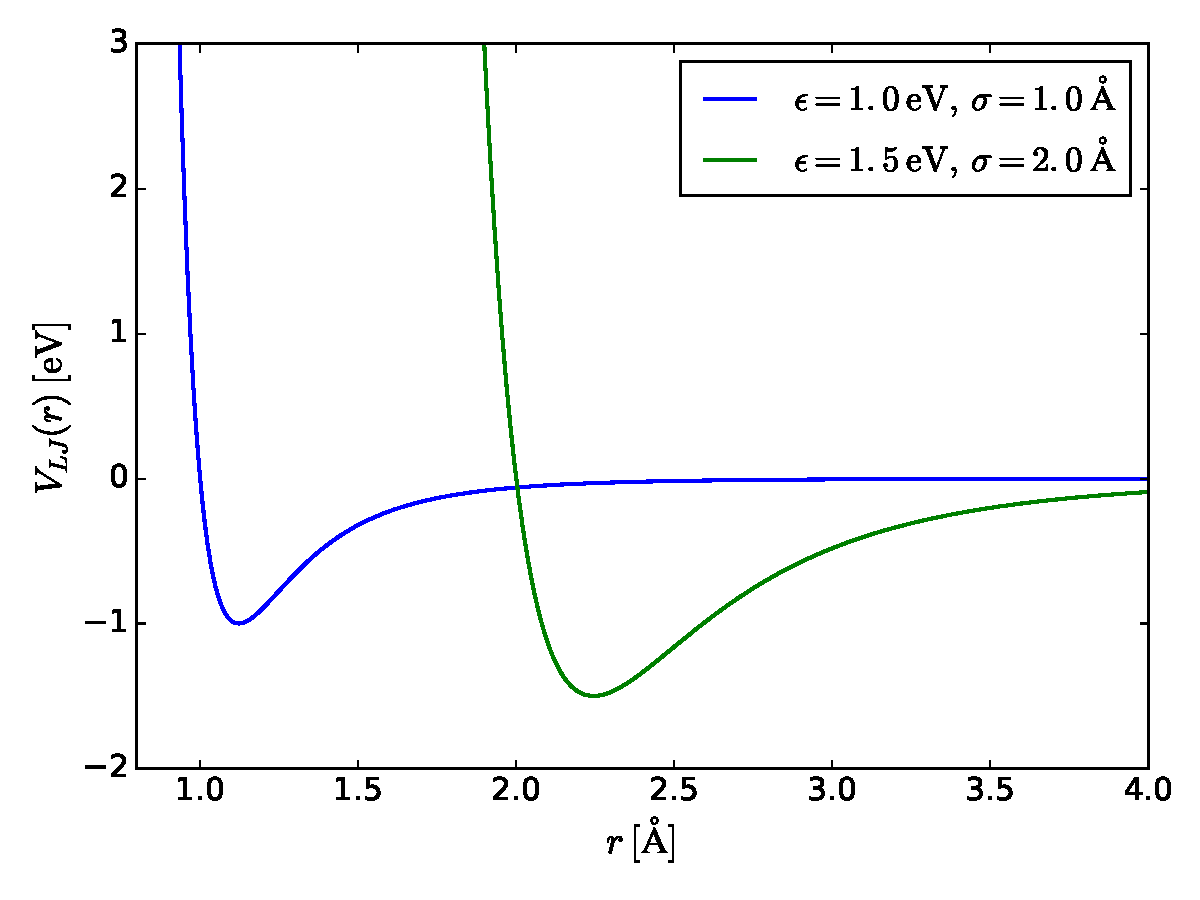
\includegraphics[width = 0.7\linewidth]{Figures/Theory/LJ.pdf}
 \caption{The Lennard-Jones potential \eqref{Lennard-Jones} as a function of inter-atomic distance for two different parameter sets. 
 The depth of the potential well (potential
 strength) is given by $\epsilon$, while $\sigma$ is the inter-atomic distance for which the potential is zero.}
 \label{fig:LJ}
\end{figure}




\subsubsection{Calculating total potential energy}
Before we move on to three-body potentials, we will briefly explain how the total potential energy of a system is calculated. 
For a two-body potential like LJ, each unique pair of atoms is only counted once, so that
\begin{equation}
 V_{\mathrm{tot}} = \sum_{i<j} V_2(r_{ij}) = \frac{1}{2}\sum_{i\neq j} V_2(r_{ij})
 \label{twoBodyPotentialEnergy}
\end{equation}
In the second expression we count all pairs twice, thus a factor $1/2$ is required. 
For the three-body case, the counting is a bit more complicated. An atomic triplet is defined by the three
variables $(r_{ij}, r_{ik}, \theta_{jik}$), where $r_{ij}$ and $r_{ik}$ are the 
two inter-atomic distances to the central atom $i$, and $\theta_{jik}$ is the angle between the lines from $i$ to $j$ and 
from $i$ to $k$. Note that there are only two \textit{independent} variables, since
\begin{equation}
 \theta_{jik} = \frac{\vec{r}_{ij} \cdot \vec{r}_{ik}}{r_{ij}^2r_{ik}^2}
\end{equation}
\autoref{fig:triplets} illustrates that three atoms $(i, j, k)$ define three different triplets depending
on which atom that is the central one. All three triplets have different energies, and must therefore be tallied individually.
If we assume that the potential form is symmetric with respect to exchange of the $j$ and $k$
indicies (which is not always the case for multielemental systems), we have
\begin{equation}
 \sum_{i<j<k}\left[V_3^{(1)}(r_{ij}, r_{ik}, \theta_{jik}) + V_3^{(2)}(r_{ij}, r_{jk}, \theta_{ijk}) + 
 V_3^{(3)}(r_{ik}, r_{jk}, \theta_{ikj})\right]
 \label{threeBodyPotentialEnergy1}
\end{equation}
\begin{figure}
 \centering
 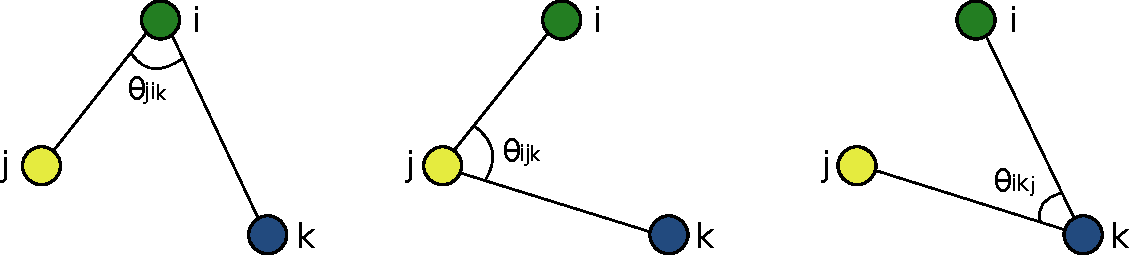
\includegraphics[width = 0.8\linewidth]{Figures/Theory/triplets.pdf}
 \caption{Three atoms $(i,j,k)$ define three different triplets that generally have different energies. They must therefore 
          be tallied individually when computing the total energy of a system.}
 \label{fig:triplets}
\end{figure}
where $V_3^{(i)}$ is one of the triplets in \autoref{fig:triplets}. Alternatively, we can calculate the energy of one triplet 
at a time and instead sum over all $j$,
\begin{equation}
 \sum_{i}\sum_{j\neq i}\sum_{k>j} V_3 (r_{ij}, r_{ik}, \theta_{jik}) 
 \label{threeBodyPotentialEnergy2}
\end{equation}
This is the convention we are going to adopt in the following. 
The total energy is now written,
\begin{equation}
 V_{\mathrm{tot}} = \sum_i\sum_{j>i} V_2(r_{ij}) + \sum_{i}\sum_{j\neq i}\sum_{k>j} V_3 (r_{ij}, r_{ik}, \theta_{jik}) 
 \label{totalPotentialEnergy}
\end{equation}


\subsection{Stillinger-Weber} \label{sec:stillingerWeber}
The Stillinger-Weber (SW) potential was proposed in 1985 \cite{Stillinger85} for simulating Si atoms. It has a two-body
and a three-body term, and is thus written on the form \eqref{totalPotentialEnergy}. 
The two-body part consists of a Lennard-Jones factor with variable exponents, together with an exponential decay factor
that ensures zeroing out of the potential at a \textit{cutoff} distance $r_c = a\sigma$,
\begin{equation}
 V_2(r_{ij}) = A\epsilon\left[B\left(\frac{\sigma}{r_{ij}}\right)^p - 
 \left(\frac{\sigma}{r_{ij}}\right)^q\right] \exp\left(\frac{\sigma}{r_{ij} - a\sigma}\right)
 \label{StillingerWeber2Body}
\end{equation}
The significance of the cutoff $r_c$ is explained in \autoref{sec:forceCutoff}. 
Silicon forms 4-coordinated
tetrahedral bonded structures, and the purpose of the three-body component is to enforce the tetrahedral bond angle
$\theta_0 \approx 109^\circ$, 
\begin{equation}
 V_3(r_{ij}, r_{ik}, \theta_{jik}) = \lambda\epsilon[\cos\theta_{jik} - \cos\theta_0]^2
 \exp\left(\frac{\gamma\sigma}{r_{ij} - a\sigma}\right)\exp\left(\frac{\gamma\sigma}{r_{ik} - a\sigma}\right)
 \label{StillingerWeber3Body}
\end{equation}
We observe that for $\theta_{jik} = \theta_0$, the three-body term is zeroed out, making this configuration energetically 
favourable. The expression also contains two exponential decay factors to ensure that the potential goes 
to zero once $r_{ij}$ and/or $r_{ik}$ approach the cutoff. 

SW simulations of solid and liquid silicon agree reasonably well with experimental data \cite{Stillinger85}.
The potential has also been used on other systems than silicon, for instance in monatomic water models \cite{Molinero08}. 

\subsection{Vashishta}
In 1990, Vashishta et al.\ \cite{Vashishta90} suggested a three-body interaction potential for $\mathrm{SiO}_2$. 
The three-body term is of similar form to that of Stillinger-Weber, 
\begin{equation}
\begin{aligned}
 V_3(r_{ij}, r_{ik}, \theta_{jik}) \: = \:
 &B_{jik}\frac{[\cos\theta_{jik} - \cos\theta_{0jik}]^2}{1 + C[\cos\theta_{jik} - \cos\theta_{0jik}]^2} \: \cdot \\
 &\exp\left(\frac{\gamma_{ij}}{r_{ij} - r_{0ij}}\right)
 \exp\left(\frac{\gamma_{ik}}{r_{ik} - r_{0ik}}\right)
\end{aligned}
\end{equation}
We note that indicies are included for the parameters, as they are generally different for each pair and triplet combination
of elements; the parameter set must be fitted to e.g.\ (Si,Si,Si) and (Si,O,O) seperately. The angle $\theta_{0jik}$ has 
the same purpose as for SW, while $r_{0ij}$ is the cutoff distance for each pair of elements. 

\noindent The two-body part is more complex,
\begin{equation}
 V_2(r_{ij}) = \frac{H_{ij}}{r^{\eta_{ij}}} - \frac{W_{ij}}{r^6} + \frac{Z_iZ_j}{r}\exp(-r/\lambda_{1,ij}) - 
 \frac{D_{ij}}{r^4}\exp(-r/\lambda_{4,ij}) 
\end{equation}
where we recognize the two first terms as typical LJ repulsive and attractive components. The other two describe
electrostatic interactions, the third being a so-called screened Coulomb potential for charges $Z_i$ and $Z_j$. 
We will not expand upon the physical justification of these terms here. 

The Vashishta potential has also been succesfully employed on other multi-component systems like SiC \cite{Vashishta07}. 


\section{Time integration} \label{sec:timeIntegration}
To evolve the system forward in time, we need a numerical method to integrate Newton's equations of motion,
\begin{align}
 \vec{v}(t) = \vec{v}(0) + \int_0^t\vec{a}(t)dt \label{equationsOfMotion1} \\
 \vec{r}(t) = \vec{r}(0) + \int_0^t\vec{v}(t)dt
 \label{equationsOfMotion2}
\end{align}
Various finite different schemes can be used for this purpose, and the choice of algorithm is 
of vital importance to the quality of the simulation. The most important property of an integrator
for use in MD, is long-term energy conservation. MD simulations are often run for millions of time steps, 
and a significant energy drift may cause useless results. Further, all integration schemes approximate 
derivatives as finite differences, introducing truncation errors. Finally, numerical stability is
important to prevent unphysical behaviour on large time scales. 

A good choice is the Velocity-Verlet algorithm, which is
a \textit{symplectic} integrator. Put simply, this means that it preserves the form of Hamilton's equations, thereby
conserving energy% 
\footnote{Strictly speaking, Velocity-Verlet only conserves a pseudo-Hamiltonian
approaching the true Hamiltonian in the limit of infinitesimal time steps \cite{Frenkel01}.}.
Employing Velocity-Verlet
allows us to sample the phase space of the microcanonical (NVE) ensemble, and collect 
thermodynamic properties like temperature and pressure.
The steps of the algorithm are,
\begin{align}
 \vec{v}(t + \Delta t/2) &= \vec{v}(t) + \frac{\vec{F}(t)}{m}\frac{\Delta t}{2} \\
 \vec{r}(t + \Delta t) &= \vec{r}(t) + \vec{v}(t + \Delta t/2)\Delta t \\
 \vec{v}(t + \Delta t) &= \vec{v}(t + \Delta t) + \frac{\vec{F}(t + \Delta t)}{m}\frac{\Delta t}{2}
\end{align}
First, the velocity at half the time step forward $\vec{v}(t + \Delta t/2)$ is computed. 
This half-velocity is used to obtain the new positions $\vec{r}(t + \Delta t)$. 
Then we calculate the new accelerations $\vec{F}(t+\Delta t)/m$ based on the new positions, which is used
to compute the velocities at a whole time step forward $\vec{v}(t + \Delta t)$. 

In addition to being symplectic, Velocity-Verlet is time-reversible \cite{Frenkel01}, which it should be considering that we 
are solving time-reversible equations (\ref{equationsOfMotion1},~\ref{equationsOfMotion2}).  
It is also computationally inexpensive; the only 
additional calculation compared to the primitive Euler method is the half-velocity. 
The global error in position and velocity is $O(\Delta t^2)$, which may not seem very impressive. However, 
this is sufficient for collecting statistical properties, 
our goal is not to reproduce the exact trajectories of the particles. 

Velocity-Verlet is the integrator of choice in LAMMPS (\autoref{sec:lammps}), and thus the 
only scheme used in this work. 

\section{Force calculations and cutoff radius} \label{sec:forceCutoff}
We need the force on each atom to compute the acceleration that is integrated in the equations of motion
(\ref{equationsOfMotion1},~\ref{equationsOfMotion2}). 
Using the Lennard-Jones potential as an example, 
the force on atom $i$ from atom $j$ is (\ref{forcePES},~\ref{Lennard-Jones}),
\begin{equation}
 F_{\mathrm{LJ}}(r_{ij}) = -\nabla V_{\mathrm{LJ}}(r_{ij}) = 
 -24\epsilon\left[2\left(\frac{\sigma^{12}}{r_{ij}^{13}}\right) - \left(\frac{\sigma^6}{r_{ij}^7}\right)\right] 
\end{equation}
The force is of the same shape 
as the potential in \autoref{fig:LJ}, which means it rapidly goes to zero. If we choose units so that
$\sigma=\epsilon=1.0$, the force at a distance $r_{ij} = 3\sigma$ is
\begin{equation}
 F_{\mathrm{LJ}}(r_{ij} = 3.0\sigma) \approx 0.01
\end{equation}
This is a general property of systems where only van der Waal-interactions are present: Atoms that 
are far apart do not effectively interact. This can be exploited in MD simulations by introducing 
a cutoff radius $r_\mathrm{c}$, and only compute forces for atoms displaced by a distance smaller than this cutoff. 
In principle, we have to sum over all pairs of atoms in the system to compute the energy and forces, which 
scales like $O(N^2)$. With a cutoff, this is reduced to $O(N)$, and the force is now written,
\begin{equation}
 F_{\mathrm{LJ}}(r_{ij}) = 
 \begin{cases}
  -24\epsilon\left[2\left(\frac{\sigma^{12}}{r_{ij}^{13}}\right) - \left(\frac{\sigma^6}{r_{ij}^7}\right)\right] ,
  & r_{ij} \leq r_\mathrm{c} \\
  0, & r_{ij} > r_\mathrm{c} 
 \end{cases}
 \label{forceCutoff}
\end{equation}
which greatly increases the computational performance of MD simulations. In fact, simulations with non-bonded potentials
not including a cutoff is unfeasible except for small systems.

The potential itself \eqref{Lennard-Jones} is also truncated at $r_{ij} = r_\mathrm{c}$, creating a discontinuity 
at the cutoff. To avoid this problem, we simply shift the LJ potential upward a little, so that the energy 
is excactly zero at this point. The truncated and shifted form of the potential is
\begin{equation}
 V_{\mathrm{LJ}}^\mathrm{trunc}(r_{ij}) = 
 \begin{cases}
  V_\mathrm{LJ}(r_{ij}) - V_\mathrm{LJ}(r_c), & r_{ij} \leq r_\mathrm{c} \\
  0, & r_{ij} > r_\mathrm{c} 
 \end{cases}
 \label{shiftedLJ}
\end{equation}






\chapter{Machine learning} \label{sec:machineLearning}
Machine learning is the science of giving computers the ability to learn without being explicitly programmed. 
The idea is that there exist generic algorithms which can be used to find patterns in a broad class of data sets without 
having to write code specifically for each problem. The algorithm will build its own logic based on the data.  

Machine learning is a subfield of computer science, and is closely related to computational statistics. 
It evolved from the study of pattern recognition in artificial intelligence (AI) research, and has made contributions to
AI tasks like computer vision \cite{Krizhevsky12}, natural language processing \cite{Collobert11}
and speech recognition \cite{Hinton12}. It has also, especially in later years, 
found applications in a wide variety of other areas, including bioinformatics, economy, physics, finance and marketing
\cite{LeCun15}. 

The approaches to machine learning are many, but are often split into two main categories. 
In \textit{supervised learning} we know the answer to a problem,
and let the computer deduce the logic behind it. On the other hand, \textit{unsupervised learning}
is a method for finding patterns and relationship in data sets withouth any prior knowledge of the system.
Some authours also operate with a third category, namely \textit{reinforcement learning}. This is a paradigm 
of learning inspired by behavioural psychology, where learning is achieved by trial-and-error, 
solely from rewards and punishment.

Another way to categorize machine learning tasks is to consider the desired output of a system.
Some of the most common tasks are:
\begin{itemize}
 \item Classification: Outputs are divided into two or more classes. The goal is to 
 produce a model that assigns inputs into one of these classes. An example is to identify
 digits based on pictures of hand-written ones. Classification is typically supervised learning.  
 \item Regression: Finding a functional relationship between an input data set and a reference data set. 
 The goal is to construct a function that maps input data to continous output values. 
 \item Clustering: Data are divided into groups with certain common traits, without knowing the different groups beforehand.
 It is thus a form of unsupervised learning.  
\end{itemize} 
\autoref{fig:machineLearningDiagram} gives an (incomplete) overview of machine learning methods with some selected applications.
We will not go into further detail on all these approaches to machine learning, as this work is only concerned with
one specific area: artificial neural networks. The rest of this chapter is devoted to the ideas behind this machine learning
approach. 
\begin{figure}
 \centering
 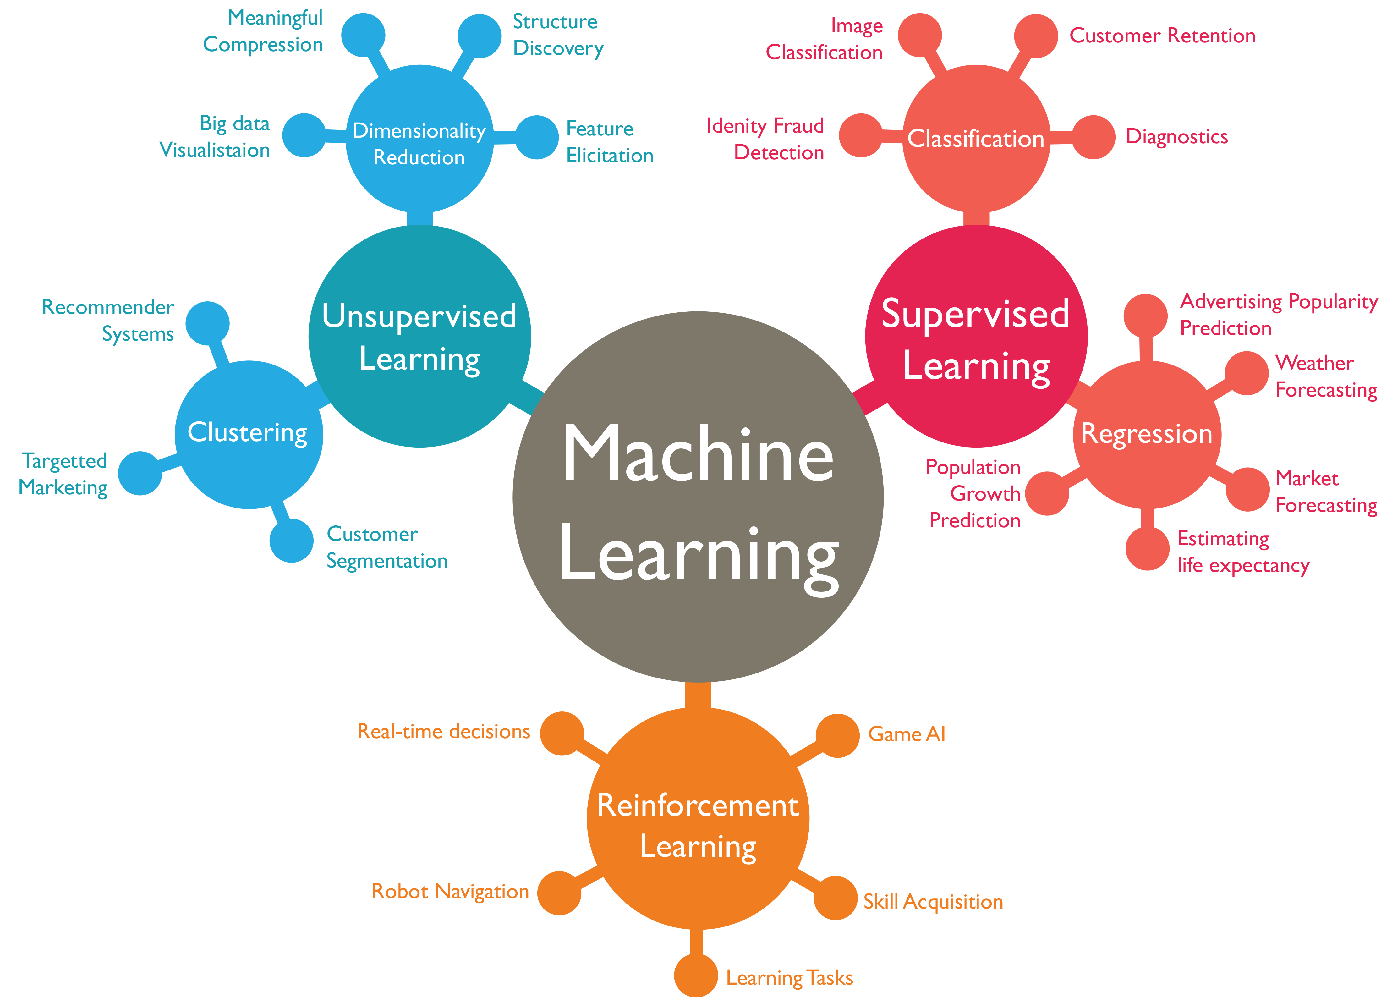
\includegraphics[width=\linewidth]{Figures/Theory/MachineLearningDiagram.png}
 \caption{Overview of various approaches to machine learning and their applications.
 Source: \href{http://www.isaziconsulting.co.za/machinelearning.html}{isaziconsulting.co.za}.}
 \label{fig:machineLearningDiagram}
\end{figure}

\section{Artificial neurons} \label{sec:ANN}
The field of artificial neural networks has a long history of development, and is closely connected with 
the advancement of computer science and computers in general. A model of artificial neurons 
was first developed by McCulloch and Pitts in 1943 \cite{McCulloch43} to study signal processing in the brain and 
has later been refined by others. The general idea is to mimic neural networks in the human brain, which
is composed of billions of neurons that communicate with each other by sending electrical signals. 
Each neuron accumulates its incoming signals, 
which must exceed an activation threshold to yield an output. If the threshold is not overcome, the neuron
remains inactive, i.e.\ has zero output.  

This behaviour has inspired a simple mathematical model for an artificial neuron \cite{Rojas96},
\begin{equation}
 y = f\left(\sum_{i=1}^n w_ix_i\right) = f(u)
 \label{artificialNeuron}
\end{equation}
Here, the output $y$ of the neuron is the value of its activation function, which have as input
a weighted sum of signals $x_i, \dots ,x_n$ received by $n$ other neurons.
The model is illustrated in \autoref{fig:neuronModel}. We will now take a closer look at if and how 
this mathematical model is biologically plausible.
\begin{figure}
 \centering
  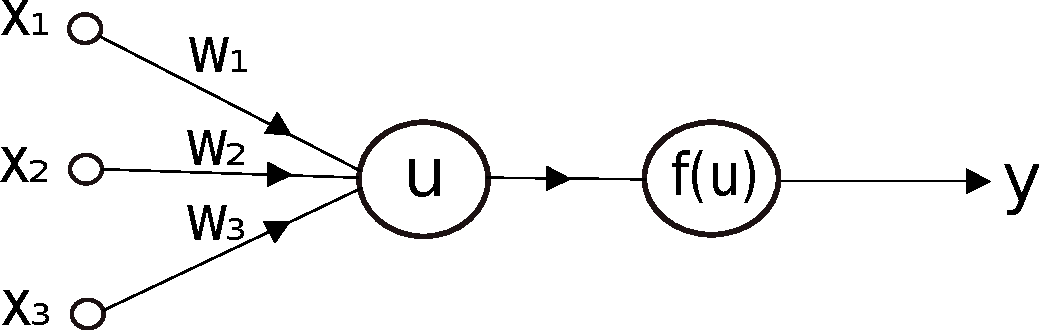
\includegraphics[width=0.8\linewidth]{Figures/Theory/neuron.pdf}
  \caption{Mathematical model of an artificial neuron. The neuron receives input signals $x_i,\dots,x_n$ from
	   $n$ other neurons. Each signal $x_i$ is associated with a weight $w_i$, and the neuron accumulates
	   all input signals as a weighted sum $u$. This sum is then used as input to its activation function
	   $f$, which serves as the neuron's output signal.}
  \label{fig:neuronModel}
\end{figure}

\subsection*{Biological model}
Artificial neurons are designed to mimic certain aspects of their biological counterparts \cite{Kriesel07}. 
A schematic model of a biological nervous cell is depicted in \autoref{fig:neuronBiological}.
The \textit{dendrites} in a neuron acts as the input vector, and allow the cell to receive signals from a large number
of neighbouring neurons. As in the mathematical model, each dendrite is associated with the multiplication of a
''weight value'', which is achieved by an increase or decrease of chemical neurotransmitters that amplifies or
weakens the input signals. The cell can also transmit signal inhibitors (oppositely charged ions) to 
accomplish ''negative'' weight values. 

The positive and negative ions arriving from the dendrites are mixed together in the solution inside the \textit{soma}, 
which corresponds to the summation in \eqref{artificialNeuron}. Finally, the \textit{axon} serves
as the activation function by sampling the electrical potential of this solution. If the potential 
reaches a certain strength, the axon transmits a signal pulse down its own length. The axon is connected 
to another neuron's dendrites (or other parts of the cell), enabling the neurons to communicate. 
\begin{figure}
 \centering
  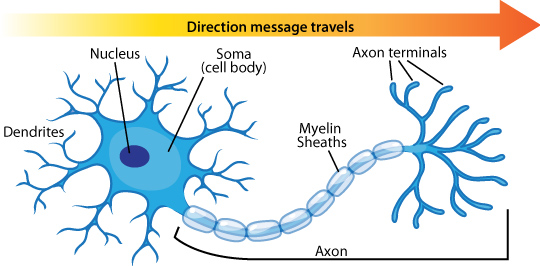
\includegraphics[width=0.9\linewidth]{Figures/Theory/neuron_anatomy.jpg}
  \caption{Biological model of a nervous cell. The various parts of the cell are briefly explained in the text. 
	   Source: \href{https://askabiologist.asu.edu/neuron-anatomy}{askabiologist.asu.edu}.}
  \label{fig:neuronBiological}
\end{figure}

This discussion of nervous cells helps, to a certain degree, to validate the mathematical form \eqref{artificialNeuron}
of artifical neurons. However, we note that the above description is a highly simplified picture of the great complexity
of biological neurons, which is not yet fully understood. Our mathematical neurons are thus only caricatures of nature. 
Next, we will look at how networks of these mathematical objects can be formed to emulate the neural networks
in the brain.

\section{Neural network types}
An artificial neural network (ANN), is a computational model that consists of layers of connected neurons, or \textit{nodes}. 
It is supposed to mimic a biological nervous system by letting each neuron interact with other neurons
by sending signals in the form of mathematical functions between layers. 
Each node is modelled according to \eqref{artificialNeuron}. 
A wide variety of different ANNs have
been developed, but most of them consist of an input layer, an output layer and eventual layers in-between, called
\textit{hidden layers}. All layers can contain an arbitrary number of nodes, and each connection between two nodes
is associated with a weight variable. 

The main factor that seperates the different types are how the neurons are \textit{connected}. 
This section contains a short presentation of some of the most common types of ANNs, before we move on to 
a more detailed description of the ANN architecture used in this thesis. In the following we will refer to artificial 
neural networks simply as neural networks (NNs), i.e.\ not referring to its biological counterpart.  

\subsection{Feed-forward neural networks}
The feed-forward neural network (FFNN) was the first and simplest type of NN devised. In this network, 
the information moves in only one direction: forward through the layers. An example FFNN is shown
in \autoref{fig:networkGeneral}, consisting of an input layer, two hidden layers and an output layer. 
Nodes are represented by circles, while the arrows display the connections between the nodes, including the 
direction of information flow. Additionaly, each arrow corresponds to a weight variable, not displayed here. 
We observe that each node in a layer is connected to \textit{all} nodes in the subsequent layer, 
making this a so-called \textit{fully-connected} FFNN. 
This is the type of NN that is used in the present work, 
and will be further investigated in \autoref{sec:MLP}.
\begin{figure}
 \centering
  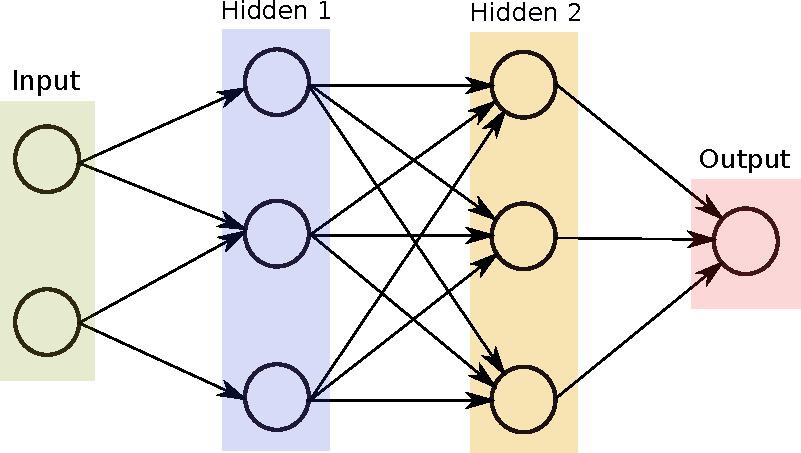
\includegraphics[width=0.8\linewidth]{Figures/Theory/networkGeneral.pdf}
  \caption{Example of a fully-connected feed-forward neural network with an input layer, two hidden layers
	   and an output layer. Each node in a layer is connected to \textit{all} nodes in the subsequent layer, 
	   and information only flows forward through the layers, hence the name.}
  \label{fig:networkGeneral}
\end{figure}

A different variant of FFNNs are \textit{convolutional neural networks} (CNNs) \cite{LeCun99}, which have a connectivity pattern
inspired by the animal visual cortex. Individual neurons in the visual cortex only respond to stimuli from
small sub-regions of the visual field, called a receptive field. This makes the neurons well-suited to exploit the strong
spatially local correlation present in natural images. The response of each neuron can be approximated mathematically 
as a convolution operation. 

CNNs emulate the behaviour of neurons in the visual cortex by enforcing a \textit{local} connectivity pattern
between nodes of adjacent layers: Each node
in a convolutional layer is connected only to a subset of the nodes in the previous layer, 
in contrast to the fully-connected FFNN in \autoref{fig:networkGeneral}.
Often, CNNs 
consist of several convolutional layers that learn local features of the input, with a fully-connected layer at the end, 
which gathers all the local data and produces the outputs. They have wide applications in image and video recognition
\cite{LeCun15}. 

\subsection{Recurrent neural networks}
So far we have only mentioned NNs where information flows in one direction: forward. \textit{Recurrent neural networks} on
the other hand, have connections between nodes that form directed \textit{cycles}. This creates a form of 
internal memory which are able to capture information on what has been calculated before; the output is dependent 
on the previous computations. Recurrent NNs make use of sequential information by performing the same task for 
every element in a sequence, where each element depends on previous elements. An example of such information is 
sentences, making recurrent NNs especially well-suited for handwriting and speech recognition.

\subsection{Other types of networks}
There are many other kinds of NNs that have been developed. One type that is specifically designed for interpolation
in multidimensional space is the radial basis function (RBF) network. RBFs are typically made up of three layers: 
an input layer, a hidden layer with non-linear radial symmetric activation functions and a linear output layer (''linear'' here
means that each node in the output layer has a linear activation function). The layers are normally fully-connected and 
there are no cycles, thus RBFs can be viewed as a type of fully-connected FFNN. They are however usually treated as
a seperate type of NN due the unusual activation functions (common activation functions are presented in
\autoref{sec:activationFunctions}).

Other types of NNs could also be mentioned, but are outside the scope of this work. We will now move on to a detailed description
of how a fully-connected FFNN works, and how it can be used to interpolate data sets. 

\section{Multilayer perceptron} \label{sec:MLP}
In this thesis we use fully-connected feed-forward neural networks with three
or more layers (an input layer, one or more hidden layers and an output layer), mainly
consisting of neurons that have non-linear activation functions.
Such networks are often called \textit{multilayer perceptrons} (MLPs)% 
\footnote{The terms ''feed-forward neural network'' and ''multilayer perceptron'' are used interchangeably in the 
literature, although the MLP is just one type of FFNN, namely a fully-connected one with mainly non-linear neurons.}.
The \textit{perceptron} was first introduced by Rosenblatt in 1958 \cite{Rosenblatt58}, and was a FFNN made up of an input layer
and an ouput layer only. It served as a \textit{binary classifier}, i.e.\ a function that maps a real-valued vector $\vec{x}$ 
to a single binary value $f(\vec{x})$, employing a linear activation function. The addition of hidden layers and 
non-linear activation functions led to the MLP, which could produce an arbitrary number of continous output values. 

\subsection{Why multilayer perceptrons?} \label{sec:whyMLP}
We have chosen to use MLPs to interpolate data sets for the construction of inter-atomic potentials. 
Other NN types could also have been used, but our choice is well justified. According to the
\textit{Universal approximation theorem} \cite{Hornik89}, a feed-forward neural network with just a single hidden layer containing 
a finite number of neurons can approximate a continous multidimensional function to arbitrary accuracy, 
assuming the activation function for the hidden layer is a ''non-constant, bounded and monotonically-increasing continous function''.
Note that the requirements on the activation function only applies to the hidden layer, the output nodes are always
assumed to be linear, so as to not restrict the range of output values. 

The only requirement on the NN information flow is that it must be feed-forward, which is not satisfied by recurrent NNs.
Anyhow, computing energies and forces in MD simulations at a given time step do not require any knowledge of 
the earlier states of the system, i.e.\ no memory or recurrency is involved.
Further, it is not obvious how local connectivity should be helpful in a MD context, thus
we might as well use the simplest multilayer FFNN available, the MLP. 

We note that this theorem is only applicable to a NN with \textit{one} hidden layer. 
Therefore, we can easily construct a NN 
that employs activation functions which do not satisfy the above requirements, as long as we have at least one layer
with activation functions that \textit{do}. Furthermore, although the universal approximation theorem
lays the theoretical foundation for regression with neural networks, it does not say anything about how things work in practice: 
A NN can still be able to approximate a given function reasonably well without having the flexibility to fit \textit{all other}
functions. 

\subsection{Mathematical model} \label{sec:MLPmodel}
In an MLP, each node (neuron) is modelled according to \eqref{artificialNeuron}. To increase the flexibility of the NN,
we also add a \textit{bias} $b$ to this model, resulting in 
\begin{equation}
 y = f\left(\sum_{i=1}^n w_ix_i + b_i\right) = f(u)
 \label{artificialNeuron2}
\end{equation}
In a FFNN of such neurons, the \textit{inputs} $x_i$
are the \textit{outputs} of the neurons in the preceding layer. Furthermore, a MLP is fully-connected, 
which means that each neuron receives a weighted sum of the outputs of \textit{all} neurons in the previous layer. 

\autoref{fig:networkNotation} displays the same NN as in \autoref{fig:networkGeneral}, now with all nodes labeled by their
output $y$, except for the input nodes, which are labeled with $x$. The input nodes are strictly speaking not 
artifical neurons, as they have no activation function. Their only purpose is to forward the NN inputs to the 
first hidden layer. A few weights $w$ (blue) and biases $b$ (green) are also included, next to the connections and nodes
which they belong to respectively. 
\begin{figure}
 \centering
  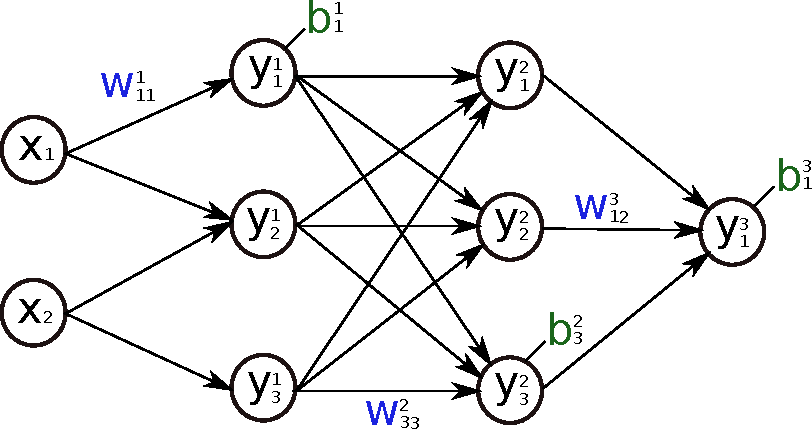
\includegraphics[width=0.8\linewidth]{Figures/Theory/networkWithNotation.pdf}
  \caption{Example of a fully-connected feed-forward neural network with an input layer, two hidden layers
	   and an output layer. Nodes are depicted as circles, while the arrows shows the connections between neurons, 
	   including their directions. Each connection has a weight $w$ (blue), where the notation explained in the
	   text is applied. Every node is marked with its output $y$ and its associated bias $b$ (green), while all input nodes
	   are labeled with an $x$. Only a few weights and biases are displayed.}
  \label{fig:networkNotation}
\end{figure}
The following notation is introduced: $y_i^l$ is the output of the $i$-th node in layer $l$, where $l=0$ is the input layer, 
$l=1$ is the first hidden layer and so on. The same notation applies to the biases. For the weights, we have that
$w_{ij}^l$ is the weight connecting node $j$ in layer $l-1$ with node $i$ in layer $l$%
\footnote{This order of indicies $i$ and $j$ may seem illogical, but will become useful when converting
to matrix equations below.}.
All weights and biases are real-valued numbers.

The MLP in \autoref{fig:networkNotation} maps the inputs $x_i$ to the output $y_1^3$ via two hidden layers
with an (arbitrary) number of hidden nodes. The hidden neurons have no physical meaning, but have the purpose
of defining the functional form of the NN. In the following we describe how to calculate the output of this MLP. The description
is also valid for a NN with several outputs; the result applies to each ouput node individually. 

First, for each node $i$ in the first hidden layer, we calculate a weighted sum $u_i^1$ of the input coordinates $x_j$,
\begin{equation}
 u_i^1 = \sum_{j=1}^2 w_{ij}^1 x_j  + b_i^1 
\end{equation}
This value is the argument to the activation function $f_1$ of each neuron $i$,
producing the output $y_i^1$ of all neurons in layer 1,
\begin{equation}
 y_i^1 = f_1(u_i^1) = f_1\left(\sum_{j=1}^2 w_{ij}^1 x_j  + b_i^1\right)
 \label{outputLayer1}
\end{equation}
where we assume that all nodes in the same layer have identical activation functions, hence the notation $f_l$%
\footnote{Note that for the activation functions, the layer indicies are subscripts rather than superscripts, 
as having a single superscript can easily be confused with a square.}.
For an arbitrary node $i$ in layer $l$ this generalizes to
\begin{equation}
 y_i^l = f_l(u_i^l) = f_l\left(\sum_{j=1}^{N_{l-1}} w_{ij}^l y_j^{l-1} + b_i^l\right)
 \label{generalLayer}
\end{equation}
where $N_l$ is the number of nodes in layer $l$. When the output of all the nodes in the first hidden layer are computed,
the values of the subsequent layer can be calculated and so forth until the output is obtained. 
The output of neuron $i$ in layer 2 is thus,
\begin{align}
 y_i^2 &= f_2\left(\sum_{j=1}^3 w_{ij}^2 y_j^1 + b_i^2\right) \\
 &= f_2\left[\sum_{j=1}^3 w_{ij}^2f_1\left(\sum_{k=1}^2 w_{jk}^1 x_k + b_j^1\right) + b_i^2\right]
 \label{outputLayer2}
\end{align}
where we have substituted $y_m^1$ with \eqref{outputLayer1}. Finally, the NN output yields,
\begin{align}
 y_1^3 &= f_3\left(\sum_{j=1}^3 w_{1m}^3 y_j^2 + b_1^3\right) \\
 &= f_3\left[\sum_{j=1}^3 w_{1j}^3 f_2\left(\sum_{k=1}^3 w_{jk}^2 f_1\left(\sum_{m=1}^2 w_{km}^1 x_m + b_k^1\right) + b_j^2\right)
  + b_1^3\right]
\end{align}
We can generalize this expression to a MLP with $l$ hidden layers. The complete functional form
is,
\begin{flalign}
&y^{l+1}_1\! = \!f_{l+1}\!\left[\!\sum_{j=1}^{N_l}\! w_{1j}^3 f_l\!\left(\!\sum_{k=1}^{N_{l-1}}\! w_{jk}^2 f_{l-1}\!\left(\!
 \dots \!f_1\!\left(\!\sum_{n=1}^{N_0} \!w_{mn}^1 x_n\! + \!b_m^1\!\right)
 \!\dots \!\right) \!+ \!b_k^2\!\right)
 \!+ \!b_1^3\!\right] &&
 \label{completeNN}
\end{flalign}
which illustrates a basic property of MLPs: The only independent variables are the input values $x_n$. 
This confirms that a MLP,
despite its quite convoluted mathematical form, is nothing more than an analytic function, specifically a 
mapping of real-valued vectors $\vec{x} \in \mathbb{R}^n \rightarrow \vec{y} \in \mathbb{R}^m$. 
In our example (\autoref{fig:networkNotation}), $n=2$ and $m=1$. Consequentially, 
the number of input and output values of the function we want to fit must be equal to the number of inputs and outputs of our MLP.  

Furthermore, the flexibility and universality of a MLP can be illustrated by realizing that 
the expression \eqref{completeNN} is essentially a nested sum of scaled activation functions of the form
\begin{equation}
 h(x) = c_1 f(c_2 x + c_3) + c_4
\end{equation}
where the parameters $c_i$ are weights and biases. By adjusting these parameters, the activation functions
can be shifted up and down or left and right, change slope or be rescaled (\autoref{fig:activationsFlex}), 
which is the key to the flexibility of a NN. 
\begin{figure}
 \centering
  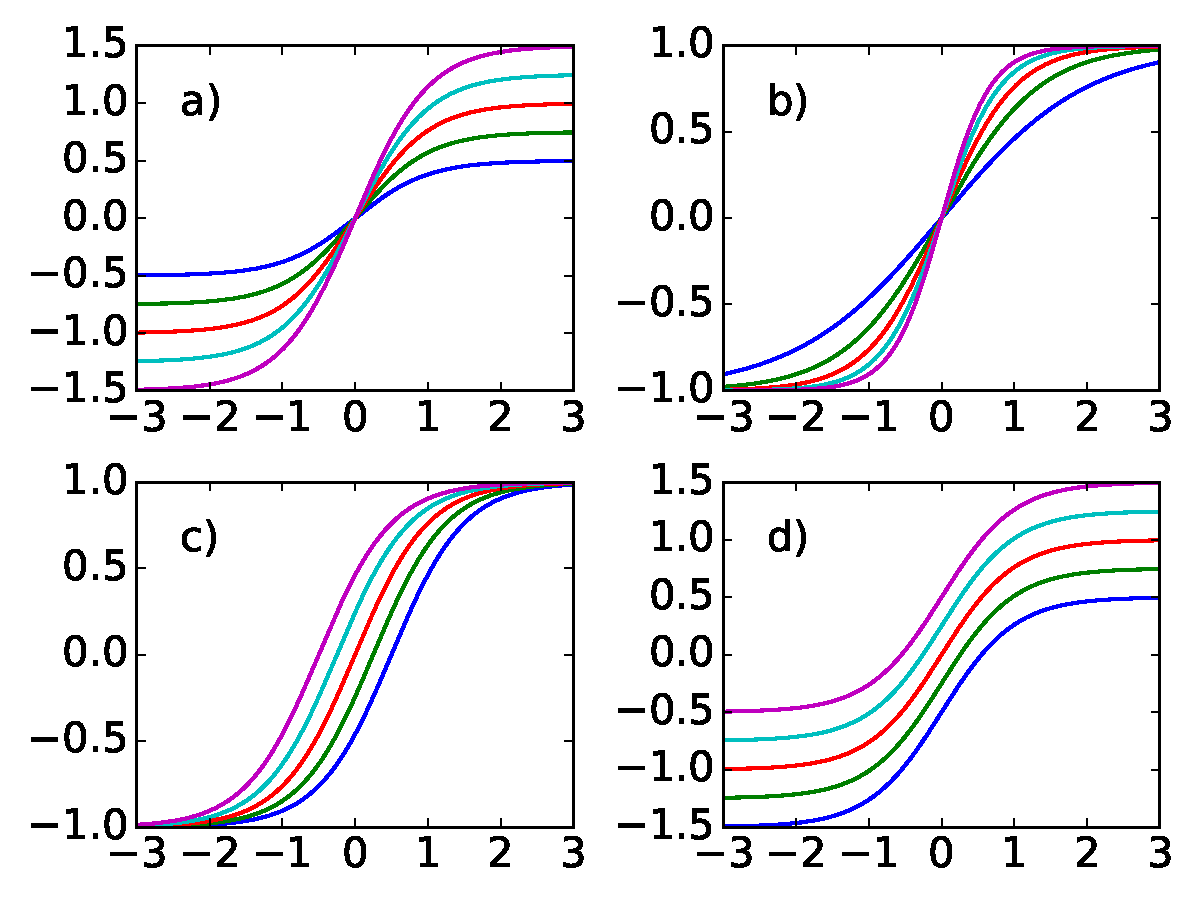
\includegraphics[width = 0.8\linewidth]{Figures/Theory/activationFlex.pdf}
  \caption{The mathematical expression for a MLP consists of nested terms of the form $h(x) = c_1 f(c_2 x + c_3) + c_4$
           \eqref{completeNN}, where $f$ is the activation function
	    and $c_i$ are NN parameters. The flexibility of the MLP is shown by adjusting $c_1$, $c_2$, $c_3$ and $c_4$ such that
	    $h(x)$ a) is scaled, b) has a change of slope, c) is shifted left and right, d) is shifted up and down, respectively. 
	    Here $f$ is the hyperbolic tangent \eqref{tanhActivationFunction}. Reproduced from Behler \cite{Behler11general}.}
  \label{fig:activationsFlex}
\end{figure}

\subsubsection{Activation function of output neuron}
We stated in \autoref{sec:whyMLP} that the output neuron always have a linear activation function for regression to avoid
restricting the output values. This is a requirement for a MLP to operate as a mapping 
$\vec{x} \in \mathbb{R}^n \rightarrow \vec{y} \in \mathbb{R}^m$. In this thesis, we will exclusively use a
specific linear activation function for the output neuron $o$, namely the identity function $f(x) = x$,
\begin{equation}
 f_o = f(u_o) = u_o
 \label{outputActivation}
\end{equation}



\subsubsection{Matrix-vector notation}
We can introduce a more convenient notation for the activations in a NN. 
If we look at the structure of the NN in \autoref{fig:networkNotation}, we realize that all the weights connecting 
two adjacent layers can be represented as a matrix $\mathrm{W}_l$, where the $(i,j)$-th element is 
is the weight $w^l_{ij}$ connecting connecting node $j$
in layer $l-1$ with node $i$ in layer $l$, as above. 

Additionaly, we can represent the biases and activations
as layer-wise column vectors $\vec{b}_l$ and $\vec{y}_l$, so that the $i$-th element of each vector 
is the bias $b_i^l$ and activation $y_i^l$ of node $i$ in layer $l$ respectively. 

We have that $\mathrm{W}_l$ is a $N_{l-1} \times N_l$ matrix, while $\vec{b}_l$ and $\vec{y}_l$ are $N_l \times 1$ column vectors. 
With this notation, the sum in \eqref{outputLayer2} becomes a matrix-vector multiplication, and we can write
the equation for the activations of hidden layer 2 in \autoref{fig:networkNotation} as%
\footnote{For the same reasons as the activation functions above, the layer indicies are changed from superscripts to subscripts
          with this matrix-vector notation.}
\begin{equation}
 \vec{y}_2 = f_2(\mathrm{W}_2 \vec{y}_{1} + \vec{b}_{2}) = 
 f_2\left(\left[\begin{array}{ccc}
    w^2_{11} &w^2_{12} &w^2_{13} \\
    w^2_{21} &w^2_{22} &w^2_{23} \\
    w^2_{31} &w^2_{32} &w^2_{33} \\
    \end{array} \right] \cdot
    \left[\begin{array}{c}
           y^1_1 \\
           y^1_2 \\
           y^1_3 \\
          \end{array}\right] + 
    \left[\begin{array}{c}
           b^2_1 \\
           b^2_2 \\
           b^2_3 \\
          \end{array}\right]\right)
\end{equation}
and we see that the activation of node $i$ in layer 2 is
\begin{equation}
 y^2_i = f_2\Bigr(w^2_{i1}y^1_1 + w^2_{i2}y^1_2 + w^2_{i3}y^1_3 + b^2_i\Bigr) = 
 f_2\left(\sum_{j=1}^3 w^2_{ij} y_j^1 + b^2_i\right)
\end{equation} 
which is in accordance with \eqref{outputLayer2}. Note that
This is not just a convenient and compact notation, but also 
a useful and intuitive way to think about MLPs: The output is calculated by a series of matrix-vector multiplications
and vector additions that are used as input to the activation functions. For each operation 
$\mathrm{W}_l \vec{y}_{l-1}$ we move forward one layer. Furthermore, it is the easiest way to implement NNs with 
TensorFlow, which is discussed in \autoref{sec:TensorFlowCreatingNN}. 



\section{Activation functions} \label{sec:activationFunctions}
A property that characterizes a NN, other than its connectivity, is the choice of activation function(s). 
As described in \autoref{sec:whyMLP}, the following restrictions are imposed on an activation function for a FFNN
to fulfill the universal approximation theorem \cite{Hornik89}:
\begin{enumerate}
 \item Non-constant
 \item Bounded
 \item Monotonically-increasing
 \item Continous
\end{enumerate}
We realize that the second requirement excludes all linear functions. Furthermore, in a MLP with only linear activation functions, each 
layer simply performs a linear transformation of its inputs. Consequentially, regardless of the number of layers, 
the output of the NN will be nothing but a linear function of the inputs. Thus we need to introduce some kind of 
non-linearity to the NN to be able to fit non-linear functions. 
\begin{figure}
\centering
  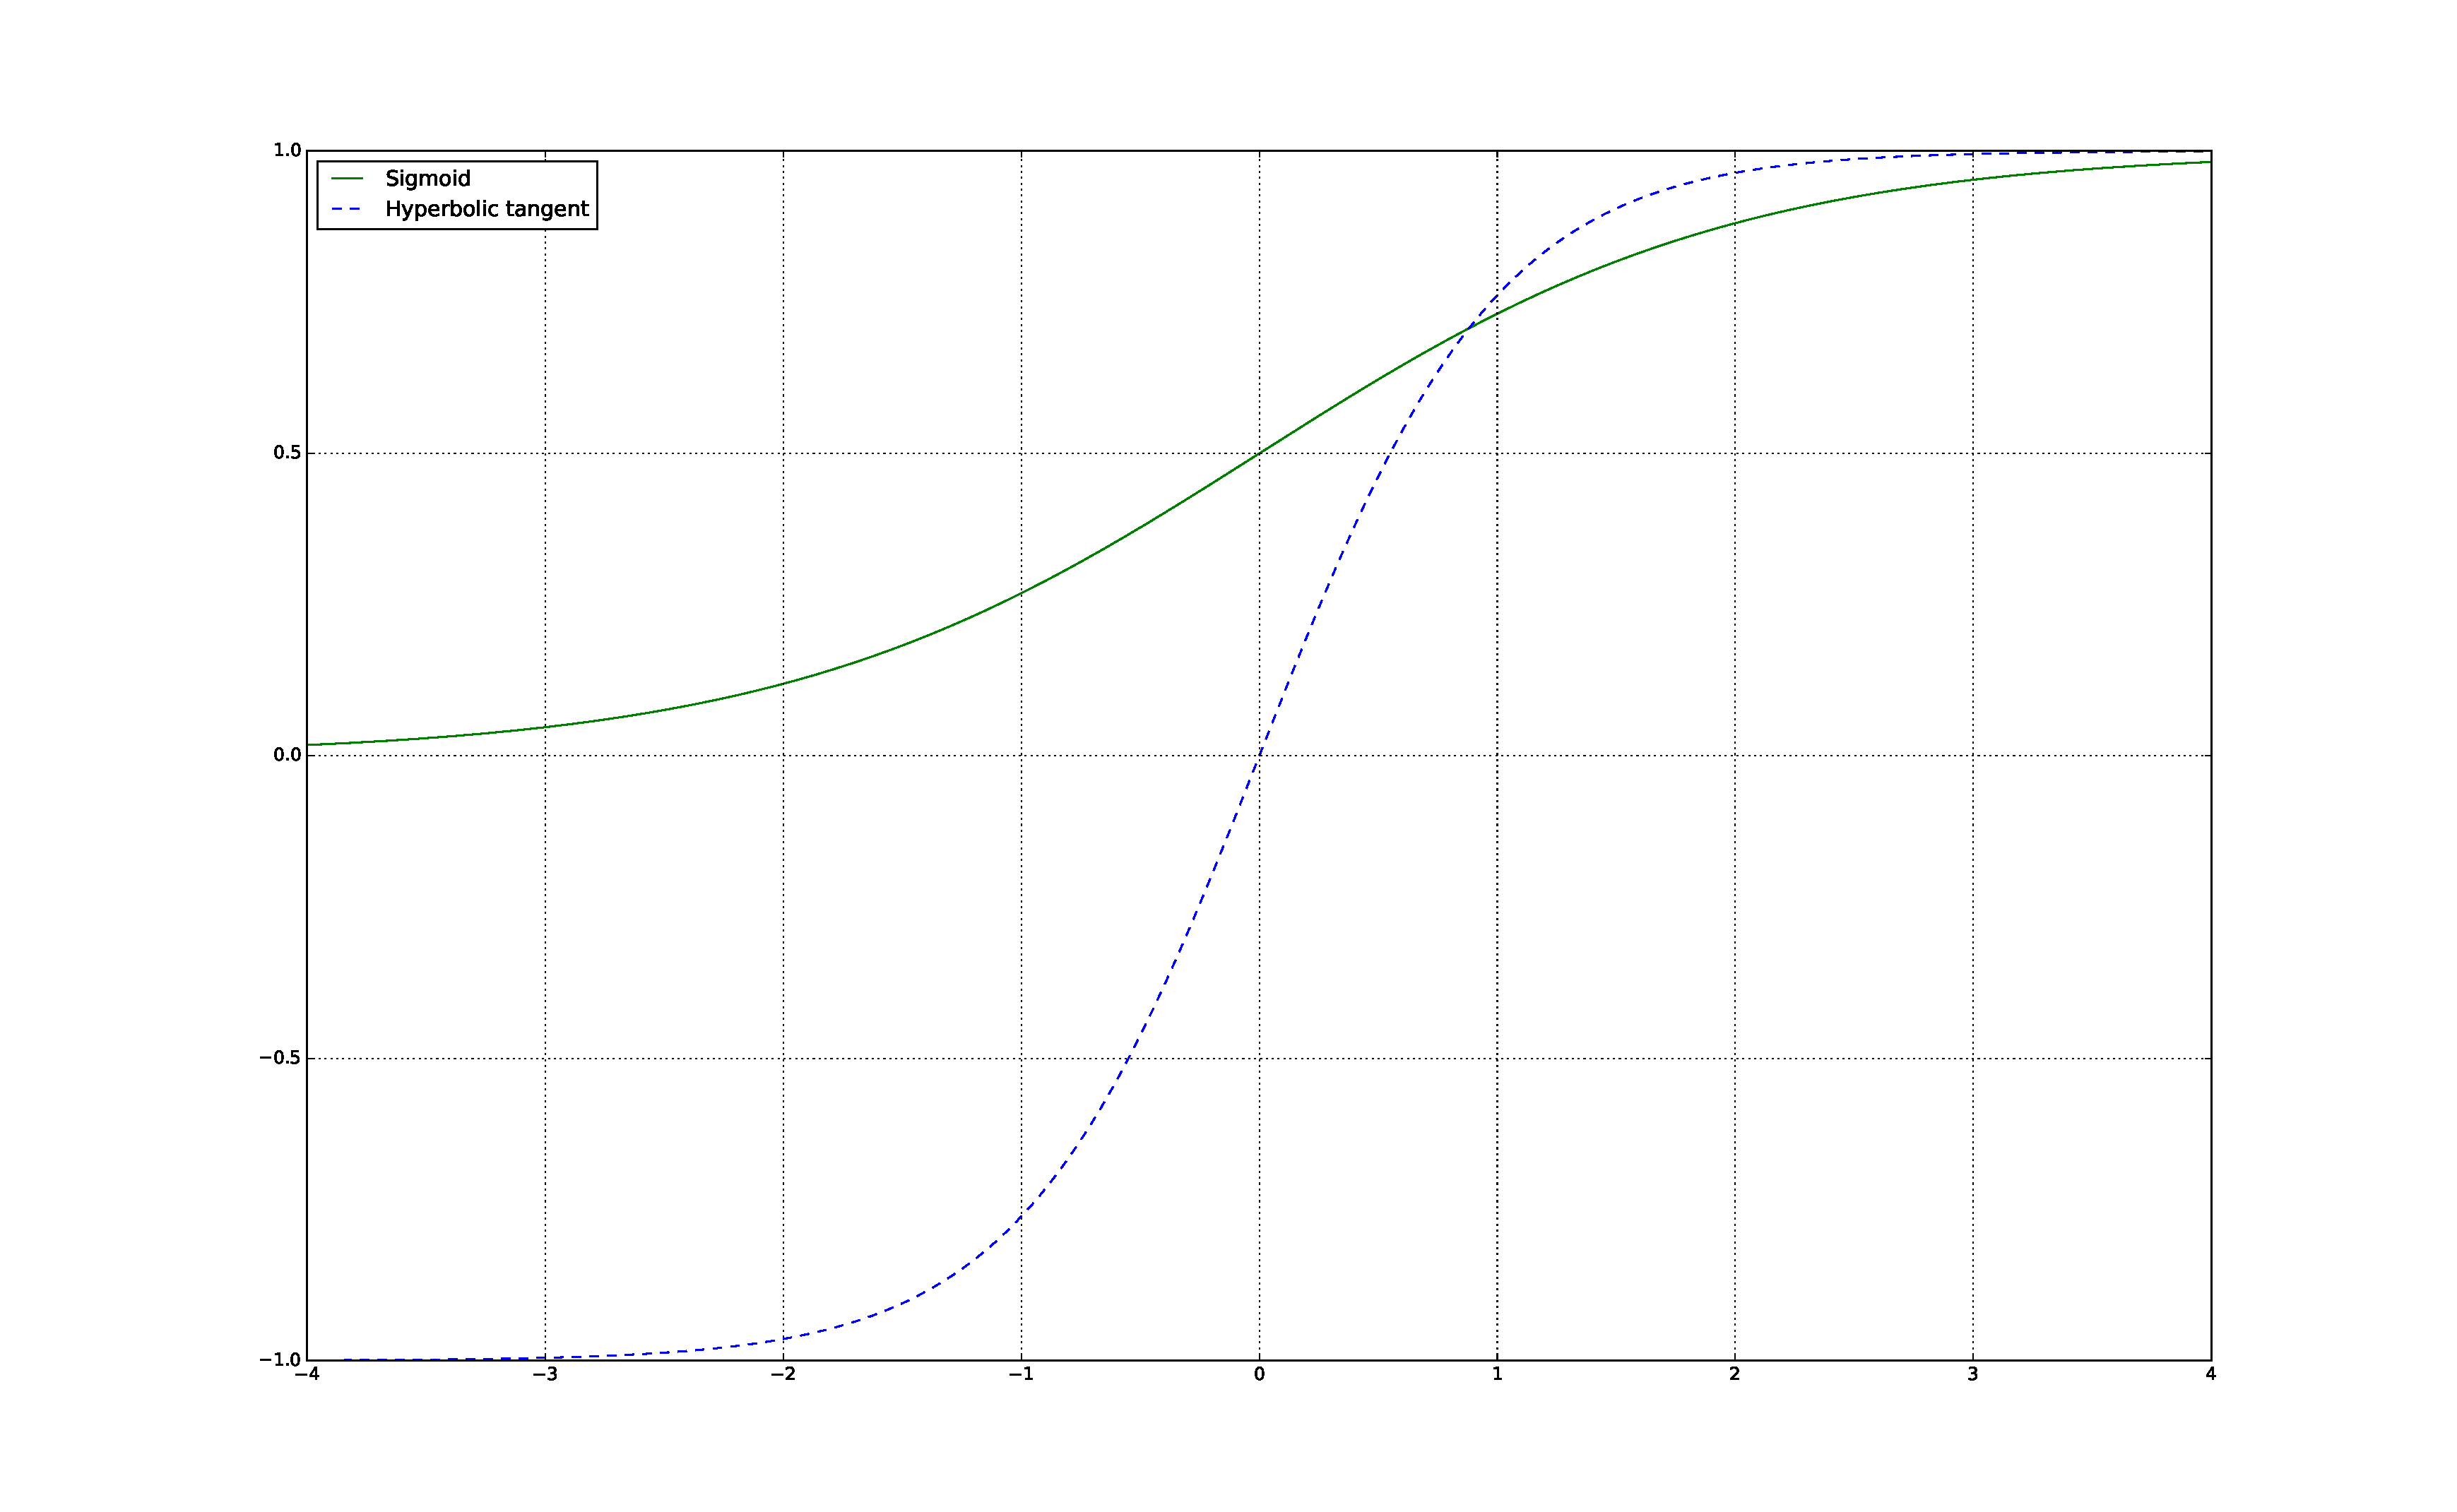
\includegraphics[width = 0.7\linewidth]{Figures/Theory/activationFunctions.pdf}
  \caption{Two of the most common activation functions for neural networks, the sigmoid \eqref{sigmoidActivationFunction} and 
           the hyperbolic tangent \eqref{tanhActivationFunction}. Both meet the requirements
	   of the universal approximation theorem.}
  \label{fig:SigmoidActivationFunctions}
\end{figure}

A group of non-linear functions that meet the above requirements are the \textit{sigmoid} functions. 
The two sigmoid functions that are most commonly used as activation functions \cite{Rojas96} in 
neural networks are the logistic function
\begin{equation}
 f(x) = \frac{1}{1 + e^{-x}}
 \label{sigmoidActivationFunction}
\end{equation}
and the hyperbolic tangent
\begin{equation}
 f(x) = \tanh(x)
 \label{tanhActivationFunction}
\end{equation}
The logistic functon is often referred to as ''the sigmoid'', which is the naming convention we will use 
in the following. Both functions are depicted in \autoref{fig:SigmoidActivationFunctions}. We observe that they
are bounded above by 1, while the lower bound is -1 and 0 for the hyperbolic tangent and sigmoid respectively. This property 
keeps the activations from diverging. 

The sigmoid are more bilogically plausible because 
the output of inactive neurons are zero. Such activation function are called \textit{one-sided}. However,
it has been shown \cite{Karlik11} that the hyperbolic tangent 
performs better than the sigmoid for training MLPs. This will be further discussed in \autoref{sec:hyperParamsActFunctions}. 
Nevertheless, one should assess the problem 
at hand when deciding what activation function to use; the performance can vary from problem to problem. 
\begin{figure}
\centering
 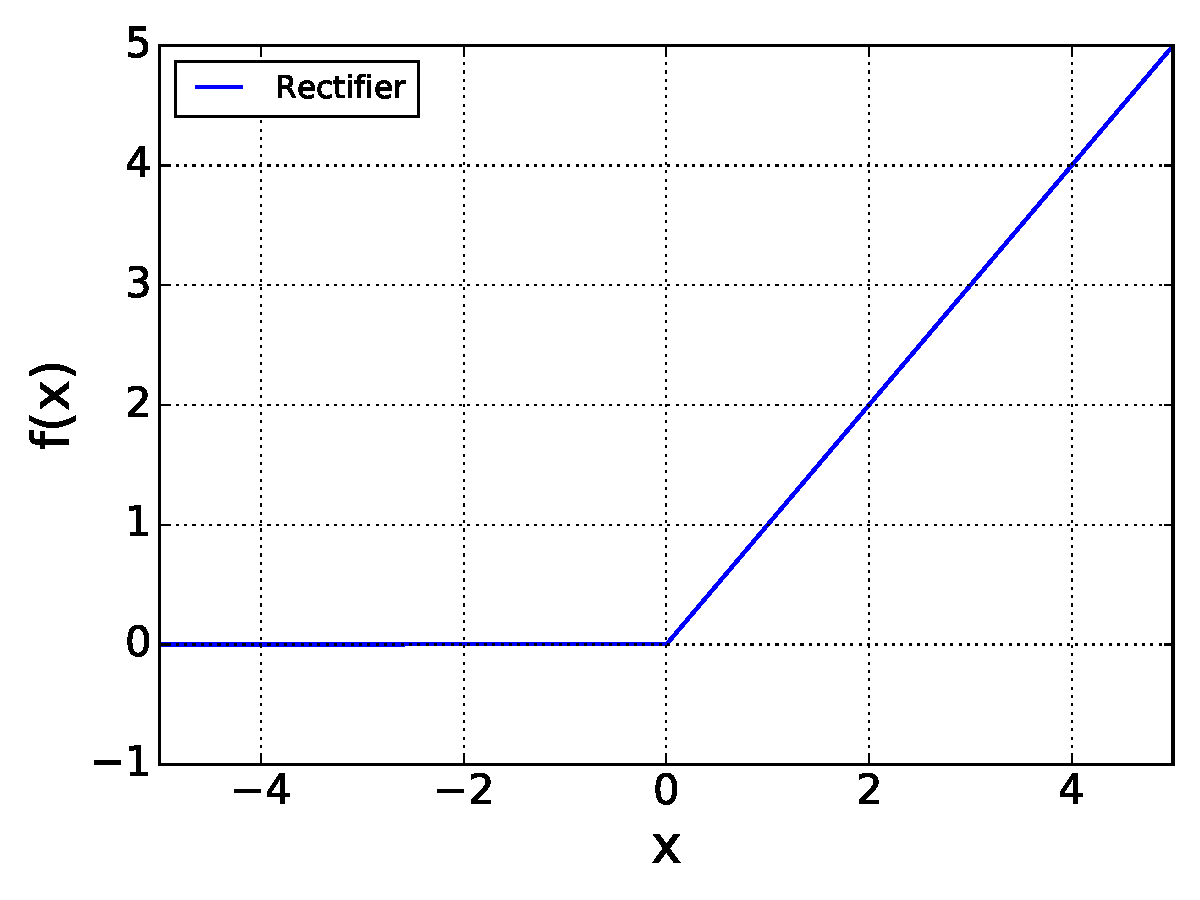
\includegraphics[width = 0.7\linewidth]{Figures/Theory/reluActivation.pdf}
  \caption{The rectifier \eqref{reluActivationFunction} has become the most popular activation function for 
           deep convolutional NNs.}
  \label{fig:reluActivationFunction}
\end{figure}

\noindent In later years, the rectifier function (\autoref{fig:reluActivationFunction})
\begin{equation}
 f(x) = \max(0,x)
 \label{reluActivationFunction}
\end{equation}
has become the most popular \cite{LeCun15} for \textit{deep neural networks}, i.e.\ NNs with several hidden layers%
\footnote{There is no consensus in the literature on how many hidden layers a NN must possess in order to qualify as ''deep'', 
but there seems to be a tendency towards setting the minimum number of layers to three.}.
It has been argued to be even more biologically plausible than the sigmoid and also perform better
than the hyperbolic tangent, especially for deep, convolutional NNs \cite{Glorot11}. Even though the rectifier is a
piecewise \textit{linear} function, it effectively behaves as a non-linearity. However, it does not have an upper bound, and
therefore does not satisfy the universal approximator requirements. Further, the function values can potentially blow up. 
These problems are solved in practice by employing various teqhniques, illustrating that the universal approximation theorem
should not be used as an absolute guideline for the construction of activation functions. 


\section{Training} \label{sec:training}
In the beginning of this chapter we defined machine learning as the ''science of giving computers the ability to learn without
being explicitly programmed.'' In the neural network case, this learning is achieved by iteratively feeding the network with data. 
With the help of certain learning algorithms, the network will then automatically adjust its parameters, i.e.\ the weights and biases, 
to find patterns in this data% 
\footnote{in the following, ''weights'' will often be equivalent to all the NN parameters, including the biases.}.
The procedure depends on what learning paradigm we work with
(unsupervised or supervised learning), and the type of NN we use. 

In this thesis we employ NNs for regression: We want to interpolate data sets og atomic coordinates and energies.
The goal is to adjust the weights of a MLP so that it accurately represents a function that maps
atomic coordinates to the corresponding potential energies. Interpolation with NNs is essentialy an optimization problem:
The weights are typically initialized as random numbers, and then modified iteratively to minimize the error
to a set of expected output values, in our case energies. 
This procedure is called \textit{training}. 

Thus, the input values to the function that we want to fit are atomic configurations,
while the output values are the total energies of these configurations. 
Together they form what we refer to as a \textit{data set} or a \textit{reference set}. 
The output values are also known as the \textit{target values}. 
The input data $\mathrm{X}$ and output data $\mathrm{Y}$ are represented as matrices, where the $i$-th row of X and Y, 
denoted $\mathrm{X}_{i*}$ and $\mathrm{Y}_{i*}$ respectively, 
together form a \textit{training example}. The combined data set consists of $N$ such training examples. 

Note that the number of columns of X and Y are equal to the number of inputs and outputs of our MLP respectively. 
This is a restatement of the observation made in \autoref{sec:MLPmodel}: The number of inputs and outputs of our MLP must be equal 
to the number of input and output values of the function we are trying to fit. In the following we assume that the MLP only has one 
output, thus each row of Y is a single number, denoted $Y_{i*} = Y_i$. 


\subsection{Cost functions} \label{costFunctions}
To minimize the error, we need a way to \textit{define} it. 
As in mathematical optimization, the error is represented by an objective function, also called \textit{loss} function
or \textit{cost} function. Training a NN therefore amounts to the minimization of this function, which can be written in the 
following general way,
\begin{equation}
 \Gamma = \Gamma\bigr(\{\mathrm{W}_l\}, \{\vec{b}_l\}, \mathrm{X}, \mathrm{Y}\bigr)
 \label{generalCost}
\end{equation}
where $\{\mathrm{W}_l\}$ and $\{\vec{b}_l\}$ are all the weights and biases of the NN respectively. 
The value of this function is a measure of how well the NN is able to map $\mathrm{X} \rightarrow \mathrm{Y}$. 
By adjusting $\{\mathrm{W}_l\}$ and $\{\vec{b}_l\}$, we try to minimize the value of this function.  

The standard cost function used in regression with NNs is the mean-square error,
\begin{equation}
 \Gamma = \frac{1}{2N}\sum_{i=1}^N (Y_i - y_i)^2
 \label{quadraticCost}
\end{equation}
where $y_i = y_i(W, B, X_{i*})$ is the value predicted by the NN for training example $X_{i*}$. 
For a MLP with more than one output, $Y_i$ and $y_i$ are vectors. 
The constant $1/2$ is included to cancel out the exponent when this function is differentiated at a later stage
(\autoref{sec:backprop}).

A variety of other cost functions are used for other machine learning tasks. In classificiation the output is often binary, 
hence the mean-square error function is inadequate. We will not go into further detail on these cost functions here, but 
\autoref{sec:hyperParamsCostFunction} provides a discussion on an extension of \eqref{quadraticCost} that is relevant for 
the construction of NNPs. 


\section{Optimization} \label{sec:optimization}
There are a large number of algorithms that can be used to determine the set of weights minimizing the 
cost function \eqref{quadraticCost}. 
Different kinds of gradient descent-based methods are widely used, while higher order methods like
the conjugate gradient algorithm or Newton's method are rarely seen in the literature because they are 
too computationally expensive for large NNs and data sets. Therefore, only first-order methods will be discussed here. 

The idea behind gradient descent methods is to minimize a function by 
iteratively taking steps in the direction of steepest descent towards a minima in parameter space. 
This direction is defined as the negative gradient of the function with respect to 
all its parameters. If we define $\vec{\theta} \in \mathbb{R}^d$ as a vector containing all the weights and biases
of a MLP, we get the following iterative scheme,
\begin{equation}
 \vec{\uptheta}_{k+1} = \vec{\uptheta}_{k} - \gamma \nabla_{\vec{\uptheta}_k} \Gamma(\vec{\uptheta})
 \label{gradientDescent}
\end{equation}
where $\gamma$ is a step size, called the \textit{learning rate} in the context of machine learning. The process is started
by initializing the parameters as random numbers. The value of $\gamma$ is of great importance for the algorithm to converge,
and is allowed to change at every iteration. Note that convergence to 
a minimum is not guaranteed withouth certain assumptions on the function $\Gamma$ and the particular choices of $\gamma$.
Also, the obatained minimum is generally local, not global. 
Different ways to update $\gamma$ is discussed below.


\subsection{Gradient descent variants} \label{sec:gradientDescentVariants}
There are three versions of gradient descent \cite{Ruder16}, which differ in 
the number of training examples we present to the NN before updating the parameters. 
According to neural network terminology, the process of adjusting the parameters based on all the training examples,
either in batches or all at once, is called an \textit{epoch}. 

In \textit{batch} gradient descent, 
we compute the gradient of the cost function for the \textit{whole} data set before updating, also called 
\textit{offline learning}. 
This approach can be very slow and is intractable for datasets that do not fit in memory. Furthermore, there is a risk
of performing redundant computations if many similar examples are present in the data set.

In contrast, \textit{stochastic} gradient descent (SDG) performs a parameter update for \textit{each} training example. 
SDG avoids redundant gradient calculations and is therefore faster than batch gradient descent. However, the accuracy 
of each update is lower compared to offline learning, which can lead to quite large error oscillations. The concept of having  
more than one parameter update per epoch is called \textit{online learning}. 

Finally, we have \textit{mini-batch} gradient descent, which is a mix of the two other approaches. The reference set 
is divided into $n$ equally sized mini-batches and a parameter update is performed for each mini-batch. This is usually the
algorithm of choice, as it has the optimal trade-off between speed and accuracy. Normal mini-batch sizes range
between 50 and 256, but should in some degree be tailored to each problem. 

We realize that SDG can be seen as 
a variant of mini-batch gradient descent with a mini-batch size of 1. In the literature, these two methods 
are often collectively referred to as SDG.


\subsection{Optimization algorithms} \label{sec:optimizationAlgorithms}
In the following we will outline different optimization algorithms that are widely used in neural network research. 
They are all variations on the update rule \eqref{gradientDescent}. The main focus of the methods is to find
a proper learning rate. A learning rate that is too small may lead to very slow convergence, while 
a learning rate that is too large can cause the loss function to fluctuate around the minimum or even diverge. 

\subsubsection{Momentum}
Near local minima, the surface area of the cost function (in parameter space) often curve much more steeply in one 
direction than in another, forming ravines. SDG will have slow converge in such regions, as it will oscillate across the slopes
while having slow progress along the bottom of the ravine. The Momentum method \cite{Qian99} avoids this problem
by accelerating SDG in the downwards direction, while damping the oscillations. The update rule is
\begin{equation}
\begin{aligned}
 \vec{v}_{k} &= \eta \vec{v}_{k-1} + \gamma \nabla_k \Gamma \\
 \vec{\uptheta}_{k+1} &= \vec{\uptheta}_k - \vec{v}_k
\end{aligned}
\label{Momentum}
\end{equation}
where $\eta$ is the momentum term, which is usually set to 0.9 or a similar value. The new update vector $\vec{v}_k$ 
is formed by adding a fraction $\eta$ of the previous update vector $\vec{v}_{k-1}$ to the gradient. In this way, the magnitude
of the update decreases for parameters (dimensions) whose gradients change direction, while it increases for parameters
whose gradients points in the same direction as in the previous step. This helps to push SDG downhill towards the minima. 

\subsubsection{Adagrad}
In SDG and Momentum, we have one learning rate $\gamma$ that is applied to all the parameters. 
Ideally, the learning rate should be adapted to each individual parameter to perform larger or smaller updates
depending on their importance. Adagrad \cite{Duchi11} does just that. For brevity, we set
\begin{equation}
 g_{k,i} = \nabla_{\theta_i} \Gamma (\vec{\uptheta})
\end{equation}
to be the gradient of the loss function w.r.t. parameter $\theta_i$ at step $k$. Adagrad adjusts the general learning rate $\gamma$
at each step $k$ for every parameter $\theta_i$ based on the past gradients for that parameter,
\begin{equation}
 \theta_{k+1,i} = \theta_{k,i} - \frac{\gamma}{\sqrt{G_{k,ii} + \epsilon}} \cdot g_{k,i}
\end{equation}
where $\mathrm{G}_k \in \mathbb{R}^{d \times d}$ is a diagonal matrix where each diagonal element $G_{k,ii}$ is the sum of squares
of the gradient with respect to $\theta_i$ up to step $k$. The smoothing constant $\epsilon \sim 10^{-8}$ is present to avoid
division by zero. The vectorized version of this equation yields,
\begin{equation}
  \vec{\uptheta}_{k+1} = \vec{\uptheta}_k - \frac{\gamma}{\sqrt{\mathrm{diag}(\mathrm{G}_k) + \epsilon}} \odot \vec{g}_k
  \label{Adagrad}
\end{equation}
where $\odot$ stands for element-wise multiplication. In other words, we do not have to manually tune the learning rate, 
Adagrad does that for us. A weakness of this method is that the learning rates inevitably shrinks for each step, 
resulting in arbitrary small values, at which point the learning stops.

For the rest of \autoref{sec:optimizationAlgorithms}, we assume for brevity that all vector operations are element-wise, i.e.\
$\vec{g}\,\vec{h} = \vec{g} \odot \vec{h}$ and $\vec{g}^2 = \vec{g} \odot \vec{g}$.

\subsubsection{Adadelta}
Adadelta \cite{Zeiler12} is an extension of Adagrad that reduces the rate at which the learning rate decreases. 
The sum of all past squared gradients is replaced by a \textit{exponentially decaying average} of all the previous squared gradients.
We introduce the vector $\vec{E}[\vec{g}^2]_k$ containing the decaying averages of the gradient
with respect to all the parameters at step $k$. 
This vector is defined recursively
as a weighted average of the previous averages $\vec{E}[\vec{g}^2]_{k-1}$ and the current gradient $\vec{g}_k$,
\begin{equation}
 \vec{E}[\vec{g}^2]_k = \eta \vec{E}[\vec{g}^2]_{k-1} + (1 - \eta) \vec{g}^2_k
 \label{decayingAverageVector}
\end{equation}
where $\eta$ is a decay constant similar to that in the Momentum method, and is usually set to the same value (0.9). 
We also define a new parameter update vector $\Delta \vec{\uptheta}_k = -\vec{v}_k$ so that
\begin{equation}
 \vec{\uptheta}_{k+1} = \vec{\uptheta}_k  + \Delta \vec{\uptheta}_k
\end{equation}
Replacing the vector $\mathrm{diag}(\mathrm{G}_k)$ in \eqref{Adagrad} with the decaying average vector \eqref{decayingAverageVector}
yields the following parameter update vector,
\begin{equation}
 \Delta \vec{\uptheta}_k = -\frac{\gamma}{\sqrt{\vec{E}[\vec{g}^2]_k + \epsilon}} \vec{g}_k
 \label{preliminiaryAdadelta}
\end{equation}
Additionally, the learning rate $\gamma$ is replaced by a decaying average of previous squared parameter updates
$\vec{E}[\Delta\vec{\uptheta}^2]$ up to step $k-1$, yielding the Adadelta update rule,
\begin{equation}
 \vec{v}_k = \frac{\sqrt{\vec{E}[\Delta\vec{\uptheta}^2]_{k-1} + \epsilon}}{\sqrt{\vec{E}[\vec{g}^2]_k + \epsilon}} \vec{g}_k
\end{equation}
The final replacement is done to obtain correct units for the update vector and to eliminate the learning rate from the equation. 
Thus, we do not even need to set a default learning rate with Adadelta. 

\subsubsection{Adam}
The final algorithm we are going to discuss is Adapte Moment Estimation (Adam) \cite{Kingma14}. This method
computes adaptive learning rates for each parameter by storing 
exponentially decaying averages of both the gradients \textit{and} 
the squared gradients \eqref{decayingAverageVector},
\begin{equation}
 \begin{aligned}
  \vec{E}[\vec{g}]_k &= \beta_1 \vec{E}[\vec{g}]_{k-1} + (1 - \beta_1) \vec{g}_k \\
  \vec{E}[\vec{g}^2]_k &= \beta_2  \vec{E}[\vec{g}^2]_{k-1} + (1 - \beta_2) \vec{g}^2_k
 \end{aligned}
\end{equation}
We set $\vec{a}_k = \vec{E}[\vec{g}]_k$ and $\vec{b}_k = \vec{E}[\vec{g}^2]_k$ so that
\begin{equation}
 \begin{aligned}
 \vec{a}_k &= \beta_1 \vec{a}_{k-1} + (1 - \beta_1) \vec{g}_k \\
 \vec{b}_k &= \beta_2 \vec{b}_{k-1} + (1 - \beta_2) \vec{g}^2_k
 \end{aligned}
\end{equation}
where $\vec{a}_k$ and $\vec{b}_k$ are estimates of the first moment (the mean) and the second moment (the uncentered variance)
of the gradients respectively, hence the name of the method. The elements of these two vectors are initialized as zeros, 
which make them biased towards zero, especially during the first time steps. This bias is counteracted by
computing bias-corrected version of the vectors (derived in \cite{Kingma14}),
\begin{equation}
 \begin{aligned}
 \hat{\vec{a}}_k &= \frac{\vec{a}_k}{1 - \beta_1^k} \\
 \hat{\vec{b}}_k &= \frac{\vec{b}_k}{1 - \beta_2^k}
 \end{aligned}
\end{equation}
The parameter update vector for Adam is obtained by replacing the gradient $\vec{g}_k$ with $\vec{a}_k$ in \eqref{preliminiaryAdadelta},
yielding the update rule,
\begin{equation}
 \vec{\uptheta}_{k+1} = \vec{\uptheta}_k - \frac{\gamma}{\sqrt{\hat{\vec{b}}_k} + \epsilon} \hat{\vec{a}}_k
 \label{adamUpdateRule}
\end{equation}
The default values of the hyperparameters are $\beta_1 = 0.9$, $\beta_2 = 0.999$ and $\epsilon = 10^{-8}$. 

\subsubsection{Which optimizer to use?}
There is no general answer to the question stated above. The adaptive learning rate methods
like Adagrad, Adadelta and Adam are generally more robust because they do not rely on manual fine-tuning of the learning rate. 
Also, an adaptive learning rate generally handles \textit{sparse} data better, i.e.\ data where some learning features
are poorly represented. 

Adam has been proven to perform favourably over the other optimization methods for certain applications like classification
with MLPs and convolutional NNs \cite{Kingma14}. However, the performance of various optimizers should be tested on 
the problem at hand to determine which method that works best. 




\subsection{Backpropagation} \label{sec:backprop}
In the preceding sections we have discussed different optimizers that implements various update rules for 
the parameters of a loss function. In our case, these parameters are the weights and biases of a neural network
and the cost function $\Gamma$ is the mean-square-error \eqref{quadraticCost}
\begin{equation}
 \Gamma = \frac{1}{2} (Y_i - y_i)^2
\end{equation}
here written as a function of only \textit{one} training example $i$. 
What we have not discussed yet, is
how we calculate the gradient of the cost function, i.e.\ how we obtain the partial derivatives $g_{ij}$ and $h_i$ 
with respect to all the weights and biases respectively,
\begin{align}
 g_{ij} &= \frac{\partial \Gamma}{\partial w_{ij}} \label{weightDerivative} \\
 h_i &= \frac{\partial \Gamma}{\partial b_i} \label{biasDerivative}
\end{align}
where we have dropped layer indicies for clarity. 
A common method to obtain these derivatives is \textit{backpropagation} \cite{Rumelhart86}. 
In backpropagation, a training example is propagated forward through the NN to produce an output. 
This output is compared to the desired output (target values), and the error is then propagated \textit{backwards}
through the layers to obtain the amount of which each parameter should be adjusted, 
hence the name.
The method is essentially an implementation of the chain rule, and will allow us to calculate
the partial derivatives of the cost with respect to all the parameters, thereby obtaining the gradient of the network. 

\subsubsection{1. Forward propagation}
The first stage of the algorithm is forward propagation, producing an output as described in \autoref{sec:MLPmodel}%
\footnote{We assume that the MLP only has one output. As before, the results are valid for each individual output in 
a many-output MLP.}.
In the following, we will use the same notation as in \autoref{sec:MLPmodel}. We also define
\begin{equation}
 A_i = \{j:w_{ij}\}
\end{equation}
as the set $\{j\}$ of nodes anterior to node $i$ and connected to node $i$ with weights $w_{ij}$, in addition to
\begin{equation}
 P_j = \{i:w_{ij}\}
\end{equation}
as the set $\{i\}$ of nodes posterior to node $j$ and connected to node $j$ with weights $w_{ij}$. 

\subsubsection{2. Backward propagation}
The second step is to backpropagate the error of the NN output. The weight derivative \eqref{weightDerivative}
can be expanded into two factors by use of the chain rule,
\begin{equation}
 g_{ij} = \frac{\partial \Gamma}{\partial u_i}\frac{\partial u_i}{\partial w_{ij}}
 \label{weightDerivativeExpanded}
\end{equation}
Now we move in the opposite direction of the feed-forward stage: First we differentiate the cost w.r.t 
the input of neuron $i$, then we differentiate the input w.r.t. weight $w_{ij}$ connecting neurons $j$ (in the preceding layer)
and $i$. 
The first term on the r.h.s. is defined as the the error $\delta_i$ of node $i$, 
\begin{equation}
 \delta_i = \frac{\partial\Gamma}{\partial u_i}
 \label{neuronError}
\end{equation}
This definition can be justified by the following argument.
To change the value of a cost function \eqref{generalCost}, we need to change the outputs of the neurons in the network. 
Changing the input $u_j$ to neuron $j$ by a small amount $\Delta u_j$ results in the output
\begin{equation}
 y_j = f_j(u_j + \Delta u_j)
\end{equation}
This change will propagate through subsequent layers in the network, finally causing the overall cost to change
by an amount $\frac{\partial \Gamma}{\partial u_j}\Delta u_j$. If $\partial \Gamma / \partial u_j$ is close to zero,
we are not able improve the cost much by perturbing the weighted input $u_j$; the neuron is already quite near the optimal value.
This is a heuristic argument for $\partial \Gamma / \partial u_j$ to be a measure of the error of the neuron. 

\noindent The second term on the r.h.s. of \eqref{weightDerivativeExpanded} is 
\begin{equation}
 \frac{\partial u_i}{\partial w_{ij}} = \frac{\partial}{\partial w_{ij}} \sum_{m\in A_i} w_{im}y_m = y_j
 \label{derivativeSecondTerm}
\end{equation}
Combining the the two terms \eqref{neuronError} and \eqref{derivativeSecondTerm} yields
\begin{equation}
 g_{ij} = \delta_i y_j
 \label{weightGradient}
\end{equation}
To compute this quantity, we thus need to know the outputs and the errors of all nodes in the network. 
The outputs are generated during the feed-forward stage \eqref{generalLayer},
\begin{equation}
 y_i = f_i(u_i) = f_i\left(\sum_{j\in A_i} w_{ij}y_j + b_i\right)
 \label{forwardProp}
\end{equation}
and need to be stored for all nodes. 
The errors are obtained by backpropagating the error of the output neuron $o$,
\begin{equation}
 \delta_o = \frac{\partial \Gamma}{\partial u_o} = \frac{\partial \Gamma}{\partial y_o}\frac{\partial y_o}{\partial u_o}
          = (Y - y_o) \frac{\partial y_o}{\partial u_o}
\end{equation}
We remember from \autoref{sec:MLPmodel} that the output neuron has the identity activation function $y_o = f_o(u_o) = u_o$, 
which reduces the error to
\begin{equation}
 \delta_o = Y  - y_o
\end{equation}
This error is then propagated backwards through the network, layer by layer. 
The error of each neuron in layer $l$ thus depends on the errors of all nerons in layer $l+1$.  
Consequentially, the error of an arbitrary hidden neuron can be written as a recursive equation (\autoref{fig:backprop}),
\begin{equation}
 \delta_j = \frac{\partial \Gamma}{\partial u_j} = 
 \sum_{i\in P_j} \frac{\partial \Gamma}{\partial u_i}\frac{\partial u_i}{\partial y_j}\frac{\partial y_j}{\partial u_j}
 \label{errorTerms}
\end{equation}
\begin{figure}
 \centering
 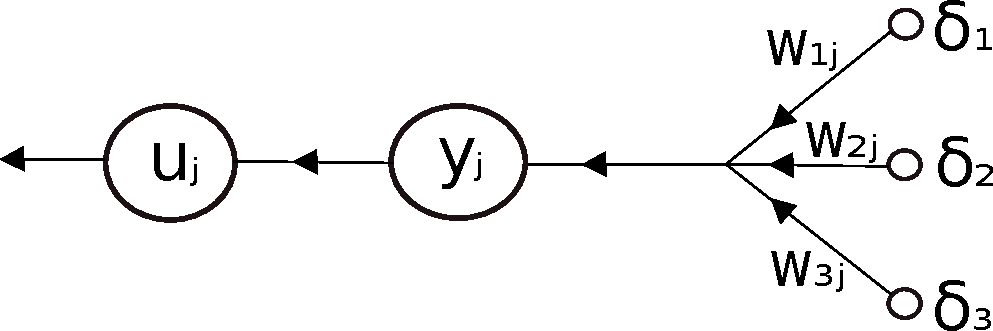
\includegraphics[width = 0.9\linewidth]{Figures/Theory/backprop.pdf}
  \caption{Illustration of the backpropagation algorithm. The direction of information flow is opposite of \autoref{fig:neuronModel}. 
	   A hidden neuron $j$ receives a weighted sum of errors of all nodes in the posterior layer. Then, we differentiate
	   in the backwards direction: the activation function (output) $y_j$ of node $j$ is differentiated w.r.t to its 
	   net input $u_j$.}
  \label{fig:backprop}
\end{figure}
We observe that also the inputs $u_i$ to all nodes need to be stored during forward propagation for 
this scheme to work. 
The first term on the r.h.s. of \eqref{errorTerms} is the error $\delta_i$ of node $i$, which is assumed to be known. 
As long as there are no cycles in the network, there is an ordering
of nodes from the output back to the input that respects this condition. It is
therefore valid only for feed-forward NNs.

The second term is the derivative of the net input of all posterior
nodes $\{i\}$ w.r.t. the output of node $j$,
\begin{equation}
 \frac{\partial u_i}{\partial y_j} = \frac{\partial}{y_j}\left(\sum_{m\in A_i} w_{im}y_m + b_i\right) = w_{ij}
\end{equation}
while the third is the derivative of node $j$'s activation function w.r.t. its net input:
\begin{equation}
 \frac{\partial y_j}{\partial u_j} = \frac{\partial f_j(u_j)}{\partial u_j} \equiv y^\prime_j
\end{equation}
Putting all the pieces together we obtain
\begin{equation}
 \delta_j = y^\prime_j\sum_{i\in P_j}w_{ij} \delta_i 
 \label{backprop}
\end{equation}
This expression is illustrated in \autoref{fig:backprop}.  
Each hidden neuron $j$ recieves a weighted sum
of the errors of all nodes in the posterior layer. Then we differentiate in the backwards direction (compare with 
\autoref{fig:neuronModel}): 
the output $y_j$ of node $j$ is differentiated w.r.t. its input $u_j$. 

The errors are propagated backwards through the whole NN until we reach the weights connecting the input layer
and the first hidden layer. 
By propagating the error
of only one ouput neuron, we thus obtain the errors of all the neurons at once. This is the main strength of the backpropagation
algorithm, and the reason for its popularity in neural network research. 

\noindent For the biases, we have \eqref{biasDerivative},
\begin{equation}
 h_j = \frac{\partial \Gamma}{\partial b_j} = \sum_{i\in P_j} \frac{\partial \Gamma}{\partial u_i}
	      \frac{\partial u_i}{\partial y_j} \frac{\partial y_j}{\partial u_j} \frac{\partial u_j}{\partial b_j}
\end{equation}
The only new term here is the last one:
\begin{equation}
 \frac{\partial u_j}{\partial b_j} = \frac{\partial}{\partial b_j}\left(\sum_{m\in A_j} w_{jm}y_m + b_j\right) = 1
\end{equation}
Consequentially, the bias gradient is simply the error of each neuron:
\begin{equation}
 h_j = \delta_j
\end{equation}

\subsubsection{Matrix notation}
In \autoref{sec:MLPmodel} we rewrote the forward propagation framework as matrix-vector equations. 
This is easily done also for the backpropagation case. From \autoref{sec:MLPmodel} we have the
set of vectors $\vec{b}_l$ and $\vec{y}_l$ for $l = 1,\dots ,L+1$, 
where $L$ is the number of hidden layers. We now extend this set with the vectors $\vec{\updelta}_l$ 
and $\vec{u}_l$, i.e.\ the errors and inputs (or \textit{preactivations}) of layer $l$
respectively. These are all column vectors of size $N_l \times 1$. 

\noindent Comparing the sums in \eqref{forwardProp} and \eqref{backprop}, we realize that since 
\begin{equation}
 \sum_j w_{ij} y_j \: \Rightarrow \: \mathrm{W} \vec{y}
\end{equation}
we have
\begin{equation}
  \sum_i w_{ij} \delta_i \:  \Rightarrow \: \mathrm{W}^T \vec{\delta}
\end{equation}
i.e.\ the weight matrices employed in backpropagation are the transpose of the matrices used in forward activation.
Thus, for nodes $\{j\}$ in layer $l$ and nodes $\{i\}$ in layer $l+1$, the vectorized equation for the error of each hidden neuron is
\begin{equation}
 \delta_j = y^\prime_j\sum_{i\in P_j}w_{ij} \delta_i \: \Rightarrow \:
 \vec{\updelta}_l = \vec{y}^\prime_l \odot (W_{l+1} \vec{\updelta}_{l+1})
\end{equation}
where $\odot$ signifies element-wise multiplication. The expression for the weight gradients \eqref{weightGradient} is converted
into an outer product of the errors of layer $l+1$ and the outputs of layer $l$,
\begin{equation}
 g_{ij} = \delta_i y_j \Rightarrow \mathrm{G}_l = \vec{\delta}_{l+1} \vec{y}^T_l
\end{equation}
where $\mathrm{G}_l$ is a matrix containing all gradients for the weights connecting layer $l$ and $l+1$. 
The corresponding matrix for the biases is a $N_l \times 1$ column vector $\vec{H}_l$,
\begin{equation}
 \vec{H}_l = \vec{\updelta}_l
\end{equation}
The set $\{\mathrm{G}_l, \vec{H}_l\}$ for $l=1,\dots,L+1$ thus make up the total gradient of the cost function \eqref{quadraticCost}. 


\subsubsection{Training algorithm}
We are now ready to express the complete training algorithm for a MLP with backpropagation using
matrix-vector notation. We introduce $\mathrm{G}_{l,i}$ and $\vec{H}_{l,i}$ as the weight gradient matrix and 
the bias gradient vector for training example $i$. 
\begin{enumerate}
 \item Input a set of $n$ training examples.
 \item For each training example $\vec{x} = X_{i*}$:
 \begin{enumerate}
 \item Initialize the input layer:
 \begin{equation}
  \vec{y}_0 = \vec{x}
 \end{equation}
 \item Propagate the activity forward. For $l = 1,\dots,L+1$:
 \begin{align}
  \vec{u}_l &= \mathrm{W}_l\vec{y}_{l-1} + \vec{b}_l \\
  \vec{y}_l &= f_l(\vec{u}_l)
  \label{forwardPropMatrix}
 \end{align}
 Store all vectors $\vec{u}_l$ and $\vec{y}_l$.
 \item Calculate and store the error in the output layer:
 \begin{equation}
  \vec{\updelta}_{L+1} = \vec{Y} - \vec{y}_{L+1}
 \end{equation}
 \item Backpropagate the error. For $l = L, L-1, \dots ,1$:
 \begin{equation}
 \vec{\updelta}_l = \vec{y}^\prime_l \odot (\mathrm{W}^T_{l+1}\vec{\updelta}_{l+1}) \cdot 
 \label{backPropMatrix}
 \end{equation}
 Store all errors $\vec{\updelta}_l$. 
 \item Compute and store the weight and bias gradients. \\ For $l = L+1, L, \dots ,1$:
 \begin{equation}
  \mathrm{G}_{l,i} = \vec{\updelta}_l \vec{y}_{l-1}^T, \quad \vec{H}_{l,i} = \vec{\updelta}_l
  \label{weightUpdate}
 \end{equation}
 \end{enumerate}
 \item Calculate the total gradients of all training examples $i$. \\
 For $l = L+1, L, \dots ,1$:
 \begin{equation}
  \mathrm{G}_l = \sum_i^n \mathrm{G}_{l,i} \quad \mathrm{and} \quad
  \vec{H}_l = \sum_i^n \vec{H}_{l,i}
 \end{equation}
 \item Update weights and biases with an update rule of choice. 
\end{enumerate}
The value of $n$ depends on the learning paradigm that is used, described in \autoref{sec:gradientDescentVariants}. 



\chapter{Neural network potentials} \label{sec:NNPs}
In \autoref{sec:constructingPES} we discussed various ways to construct a PES for use in molecular dynamics, and
stated that this thesis deales with neural network potentials (NNP). Then, in \autoref{sec:machineLearning}
we outlined the basic theory of MLPs, which is our choice of neural network type. In this chapter, 
we will discuss the symmetry problems that arise when constructing NNPs, and introduce the Behler-Parrinello method for 
solving these symmetry issues. 

\section{Neural network potentials}
NNPs are constructed by fitting an analytic function to a set of reference data
obtained by quantum mechanical calulations.
The main goal of the NN approach to constructing a PES, is to create a potential that has the accuracy of \textit{ab inito}
methods and the speed of empirical potentials (or at least of the same order).

Several different methods have been developed to construct NNPs. A comprehensive review of many of these 
has been written by Behler \cite{Behler11general}. They mainly differ in the number of NNs that are employed 
to represent the total energy of the system, the dimensionality of each NN and the choice of input coordinates. 
By dimensionality we mean the number of input nodes, as the number of output nodes is assumed to be 1 if not specified otherwise. 

\subsection{Potentials using single neural network}
In the literature, the dominant part of NN potentials employ a single feed-forward NN to calculate the total energy of the system.
This is the most straightforward approach and is the easiest to implement.
For instance, Agrawal et al.\ \cite{Agrawal06} have used a single, three-dimensional NN to study the dissociation of the 
$\mathrm{SiO}_2$ molecule. However, these types of NNPs suffer from a number of limitations. Most importantly, 
they have a fixed dimensionality. This is a general property of MLPs where the atomic coordinates are fed directly 
to the network without any transformations: Once fitted, the NNP can only be applied to systems with the same number of atoms
as the number of inputs. Further, a large number of input nodes requires many hidden neurons, and there comes a point 
where the number of parameters of the NN makes training unfeasible. Thus, the number of degrees of freedom of the system 
must be small. 

\subsection{Potentials using multiple neural networks}
For NNPs to be recognized as competitive potentials in molecular dynamics, they should be applicable to large systems
of various sizes, containing thousands of atoms. This can not be achieved by employing only one NN to 
represent the total energy of the system. A solution is to replace the single NN by a set of \textit{atomic} NNs, where 
each NN provides the contribution $E_i$ of \textit{one} atom to the total energy $E$ of the system, 
\begin{equation}
 E = \sum_{i=1}^N E_i
 \label{systemEnergy}
\end{equation}
Two methods using this approach have been developed in parallel by Bholoa et al.\ \cite{Bholoa07}, and Behler and Parrinello 
\cite{Behler07}.
Both methods compute $E_i$ based on the chemical environment of atom $i$, but they differ in how 
the environment is represented and also how the atomic NNs are structured. 

Bholoa et al.\ compute each atomic energy $E_i$ by a NN of variable size, using a set of 
vectors as input to the NN. Each vector specifies the geometry of a four atom chain $i-j-k-l$ describing the chemical 
environment. The input layer and first hidden layer are replicated once for each vector, thus the problem 
of fixed dimensionality is solved. 

Behler and Parrinello have developed a different approach to constructing a NNP. 
We have chosen to use the Behler-Parrinello (BP) method in this thesis, which will be the topic of the 
rest of the chapter. 

\section{The Behler-Parrinello method}
In the Behler-Parrinello method, the architecture of each NN is fixed, and
the atomic energies $E_i$ depend on the local chemical environments up to a cutoff radius $R_c$. 
This is analogous to the introduction of a cutoff radius in MD simulations
(\autoref{sec:forceCutoff}). Thus, the NNP can be applied to MD simlulations in excactly the same way 
as ordinary, empirical potentials: It is simply an analytic function that yields the potential energy of a central atom
in the presence of neighbouring atoms contained in a cutoff sphere of radius $R_c$. 
In other words, the BP method employs an \textit{atom-centered} approach. 
In the following we will refer to all atoms inside the cutoff sphere of an atom $i$ as \textit{neighbours}.

The cutoff is introduced by a set of so-called symmetry functions. 
These functions
describe the local chemical environment of an atom $i$ by transforming the cartesian coordinates of \textit{all} its neighbours to 
a predefined number of function values, forming a symmetry vector. 
The symmetry vector is used as input to the atomic NN of atom $i$, that in turn calculates its potential energy $E_i$.
The length of this vector must therefore be equal to the number of NN inputs. 

Each atom has an individual atomic NN along with a fixed set of symmetry functions, but
all atoms of the same element have identical 
atomic NNs and symmetry functions sets. Thus, for a diatomic system, only two unique NNs need to be trained. 

As an example, let us look at a system containing two different elements: Si and O. 
All Si atoms have idential atomic NNs and symmetry function sets, the former represented by the function $F_{\mathrm{Si}}$. 
A given Si atom $i$ has at a given time $n$ neighbours, including both Si and O atoms.  
We define $\vec{r}_{ij} = (r_{i1}, r_{i2}, \dots, r_{in})$ as the vector containing the distances from
atom $i$ to all neighbours $j = 1,\dots,n$, where $r_{ij} = |\vec{r}_j - \vec{r}_i|$. 
Further, $\vec{G}_\mathrm{Si}(\vec{r}_{ij}) = \{G_{\mathrm{Si},s}(\vec{r}_{ij})\}$ is the vector of Si symmetry functions
$s = 1,\dots,M_\mathrm{Si}$% 
\footnote{This notation signifies that each symmetry function, i.e.\ each element of 
the symmetry vector, depends on the coordinates of all atoms in the cutoff sphere. However, it does not say anything about
the form of the dependence, e.g.\ if it involves triplets or just pairs of atoms etc.}.
The process of calculating the potential energy $E_i$ described above can then be written,
\begin{equation}
 \vec{r}_{ij} \rightarrow \vec{G}_\mathrm{Si}(\vec{r}_{ij}) \rightarrow F_\mathrm{Si}[\vec{G}_\mathrm{Si}(\vec{r}_{ij})] 
 \rightarrow E_i
 \label{BPatomicEnergySi}
\end{equation}
To obtain the corresponding expression for an O atom, we simply substitute $\mathrm{Si} \rightarrow \mathrm{O}$. 
The expression is valid for any element e, and for a system with an arbitrary number of elements,
\begin{equation}
  \vec{r}_{ij} \rightarrow \vec{G}_\mathrm{e}(\vec{r}_{ij}) \rightarrow F_\mathrm{e}[\vec{G}_\mathrm{e}(\vec{r}_{ij})] 
 \rightarrow E_i
 \label{BPatomicEnergy}
\end{equation}
While the symmetry function vector of an element e is of a fixed size equal to the number of inputs to $F_\mathrm{e}$,
the length of $\vec{r}_{ij}$ can be arbitrary. This is enabled by the functional form of the symmetry functions, 
which is the topic of the next section. 

We note that although the NNs and the symmetry vectors
are identical for all atoms of the same element, the resulting energies $E_i$ are not equal since 
they depend on the unique atomic environments $\vec{r}_{ij}$ of each atom. 




\subsection{Symmetry functions} \label{sec:symmetryFunctions}
We have mentioned two requirements that the symmetry function set have to meet. First, they must contain a cutoff $r_c$
that defines a chemical environment. Secondly, since we employ atomic NNs with a fixed number of inputs,
they have to be able to produce a constant 
number of function values independent of the number of neighbours, which can change during MD simulations. 

In addition to this, the NN has symmetry problems. It does not take into account that exchanging two or more atoms
can lead to an energetically equivalent configuration. For example, exchanging the positions of both hydrogen atoms
in a water molecule will not alter the energy. However, noting that all weights have numerically different values,
changing the order of the input coordinates to the NN will result in a different energy value. This problem can be solved
by employing symmetry functions that are invariant with respect to the order of the atoms. 

Further, the energy of a system is invariant under a translation or rotation. Cartesian coordinates can therefore not be used 
directly as input to the NN, as their numerical values change under such operations, resulting in a different NN output. 

We start with defining the chemical environments by introducing a cutoff function \cite{Behler11symmetry},
\begin{equation}
 f_c(r_{ij}) = 
\begin{cases}
0.5 \!\left[\cos\left(\frac{\pi r_{ij}}{r_c}\right) + 1 \right], & r_{ij} \leq r_c \\
0, & r_{ij} > r_c
\end{cases}
\label{cutoffFunction}
\end{equation}
which is the monotonically decreasing part of a cosine function on $r_{ij} \in [0,r_c]$ (\autoref{fig:cutoffFunction}). 
\begin{figure}
 \centering
  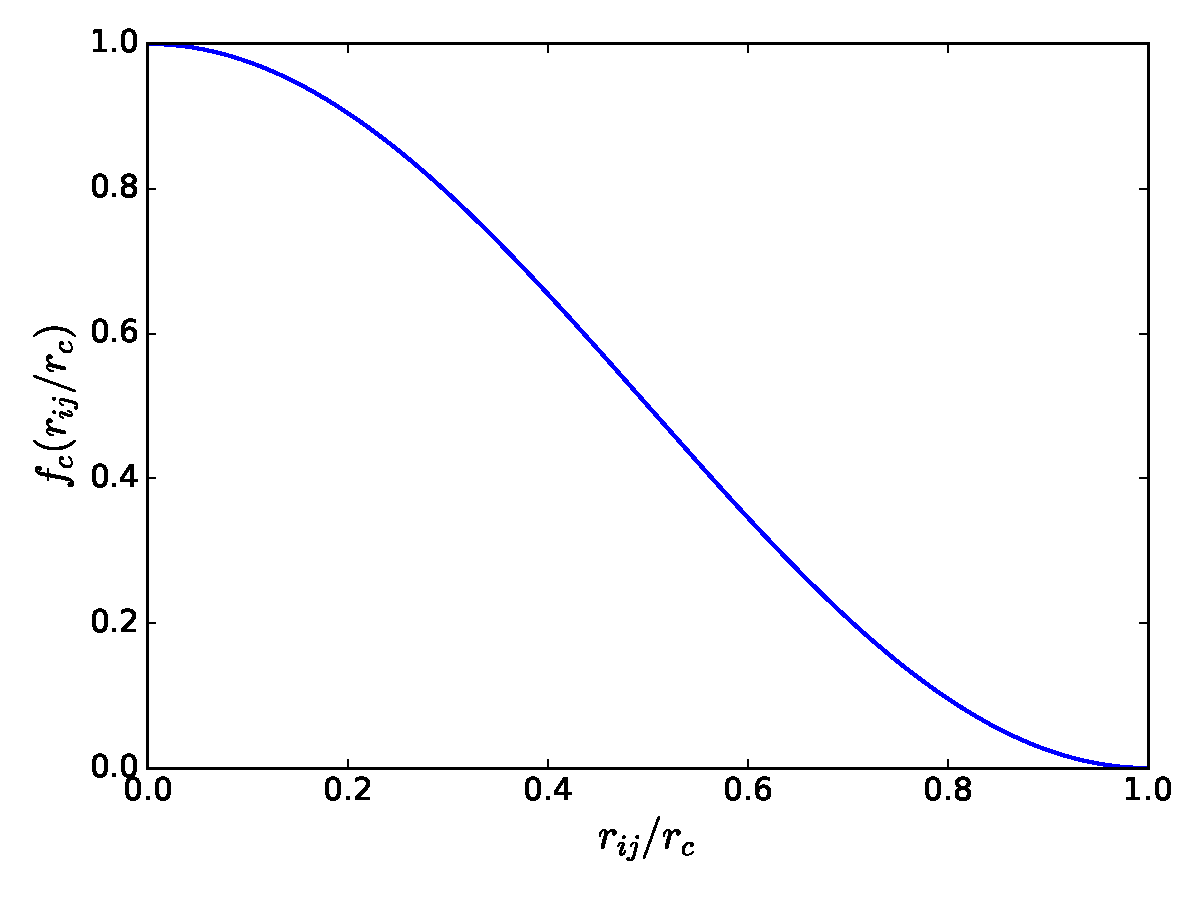
\includegraphics[width = 0.7\linewidth]{Figures/Theory/cutoffFunction.pdf}
  \caption{Plot of the cutoff function \eqref{cutoffFunction} applied in this thesis. 
	   This function is used to define a chemical environment around a central atom:
           only the atoms within the cutoff radius $r_c$ contribute to its energy. 
           These are called neighbouring atoms. The closer a neighbouring atom is, the larger
           the energy contribution, as is the case for most physical systems.}
  \label{fig:cutoffFunction}
\end{figure}
This function have the desirable property that it decreases with increasing distance $r_{ij}$ between the central
atom $i$ and its neighbour $j$. At the cutoff radius $r_c$, is has zero value and slope, which is important
to avoid discontinuities when computing energies and forces. Atoms beyond the cutoff radius are not a part of the central
atom's chemical environment and therefore do not contribute to its energy. 

Several types of many-body symmetry functions can be
constructed based on the cutoff function \eqref{cutoffFunction}. 
They can be divided into two classes: \textit{Radial} symmetry functions, describing 
the radial distribution of neighbours up to the cutoff radius, and \textit{angular} symmetry functions, specifying their
angular arrangement. The symmetry functions discussed in this section are all suggested by Behler \cite{Behler11symmetry}. 

\subsubsection{Radial symmetry functions}
The most basic radial symmetry function is simply the sum of the cutoff functions for all the neighbours $j$ of 
atom $i$,
\begin{equation}
 G_i^1 = \sum_{j=1}^N f_c(r_{ij})
 \label{G1}
\end{equation}
We immidiately realize that this simple function meets the symmetry requirement stated above: The value 
of the sum is independent of the order of neighbours $j$. This is the case for each of the following symmetry functions, as they 
are all defined as sums over neighbours. We also note that all symmetry functions, including the cutoff function, 
are unitless. 

Physically, \eqref{G1} can be thought of as a ''coordination number'' on $r_{ij} \in [0,r_c]$.
A set of such functions with different cutoff radii $r_c$ can be used to describe the radial arrangement of the neighbouring atoms by
yielding coordination numbers on distance intervals of varying length. Thus, a symmetry function is defined by 
its parameter values, 
and a set of symmetry functions with different parameters form a symmetry vector $\vec{G}$. 

A better alternative is to use a sum of products of Gaussians and the cutoff function, 
\begin{equation}
 G_i^2 = \sum_{j=1}^N \exp[-\eta(r_{ij}-r_s)^2] \,f_c(r_{ij})
 \label{G2}
\end{equation}
We now have two parameters that can be adjusted to probe different radii. The width parameter $\eta$ determines the 
radial extension of the symmetry functions, while the shifting parameter $r_s$ displaces the Gaussians to improve
the sensitivity at specific radii. A third option is 
\begin{equation}
 G_i^3 = \sum_{j=1}^N \cos(\kappa r_{ij}) \, f_c(r_{ij})
 \label{G3}
\end{equation}
which are damped cosine functions with a period length adjusted by parameter $\kappa$. We will however not use 
this function because of the existence of negative function values, which can lead to atoms canceling each other's
contribution to the sum. 

In \autoref{fig:radialSymmetriFunctions} we see the radial symmetry functions for several
different parameters. It is clear that a set of such functions can exhibit a large flexibility by tuning the parameters,
enabling us to adequately represent the radial distribution of neighbours around a central atom. 
\begin{figure}
  \begin{subfigure}{0.5\linewidth}
    \centering
    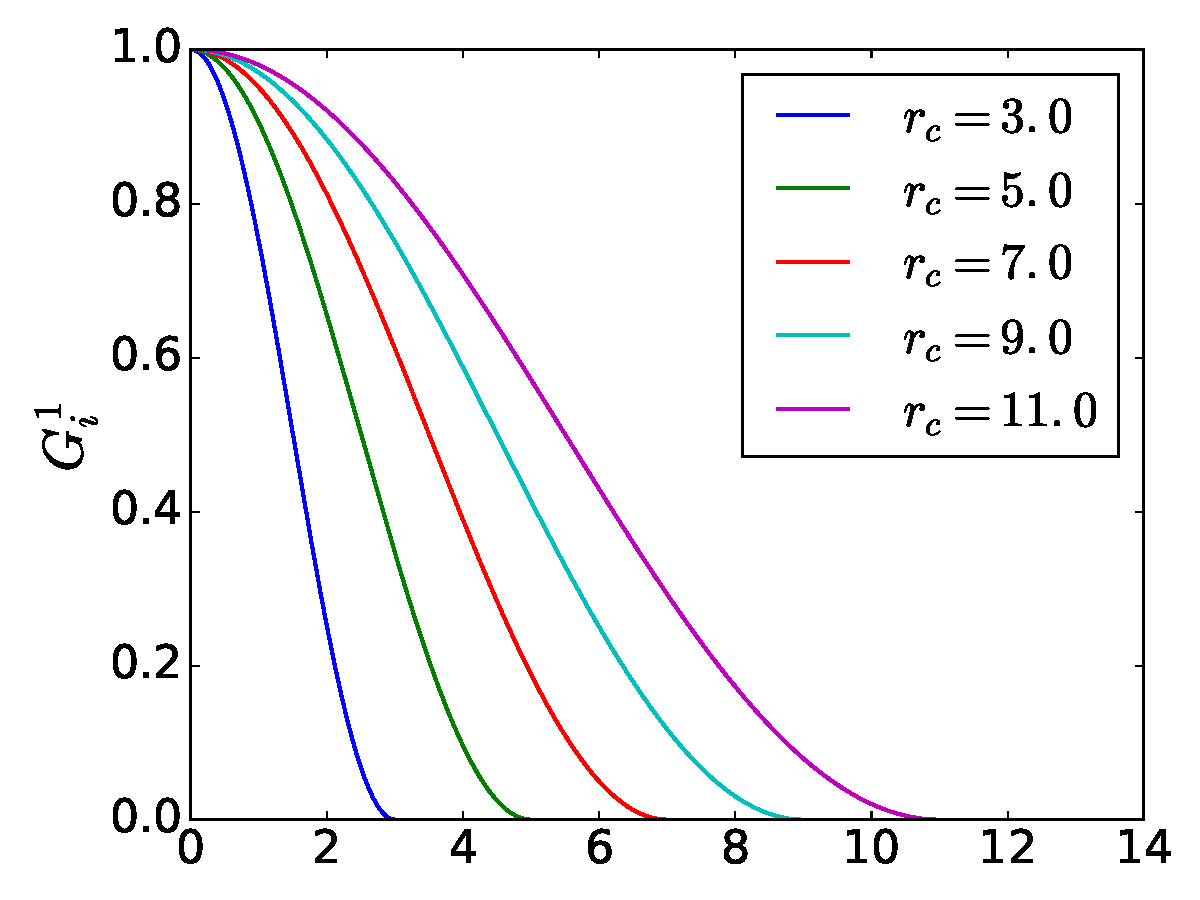
\includegraphics[width=\linewidth]{Figures/Theory/G1.pdf} 
    \label{fig:radialSymmetriFunctions:a} 
    %\vspace{1ex}
  \end{subfigure}%% 
  \begin{subfigure}{0.5\linewidth}
    \centering
    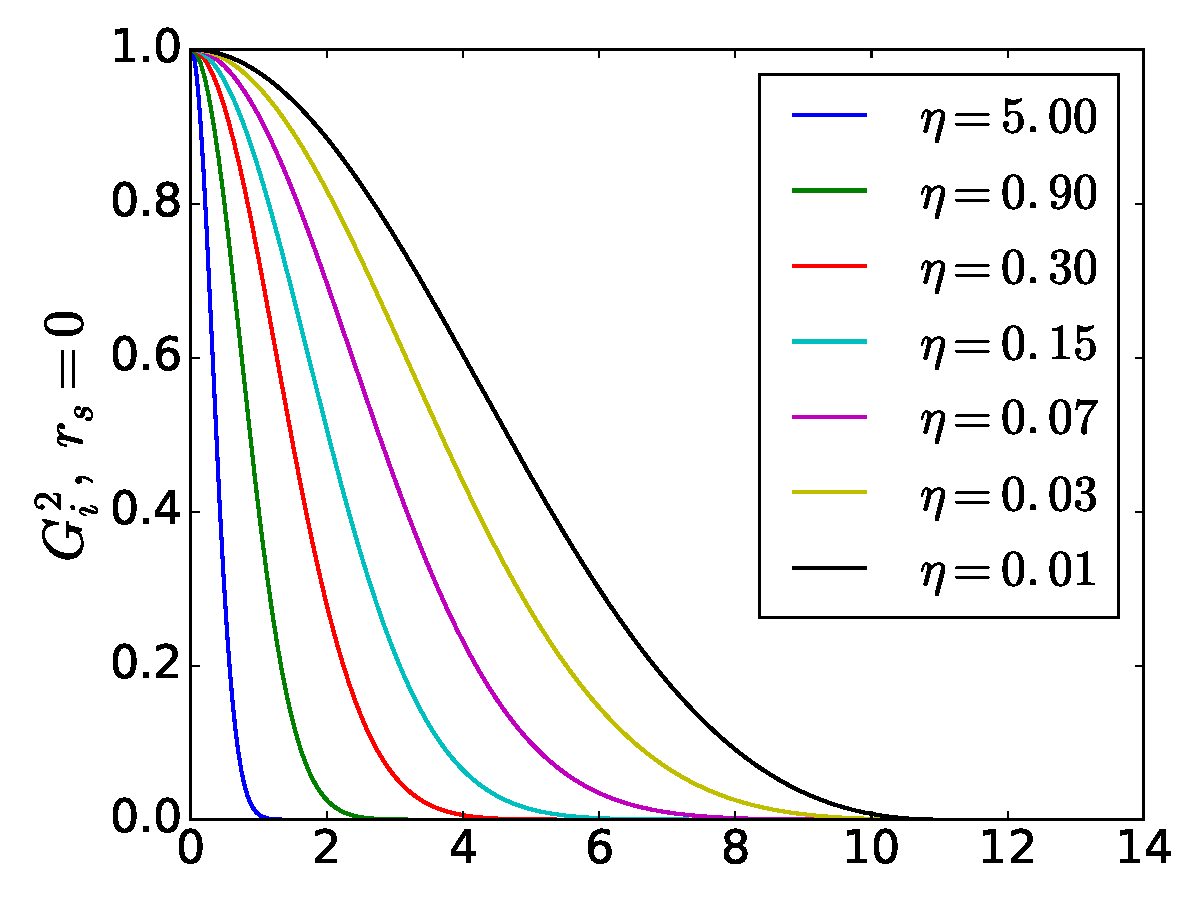
\includegraphics[width=\linewidth]{Figures/Theory/G2_1.pdf} 
    \label{fig:radialSymmetriFunctions:b} 
    %\vspace{1ex}
  \end{subfigure} 
  \begin{subfigure}{0.5\linewidth}
    \centering
    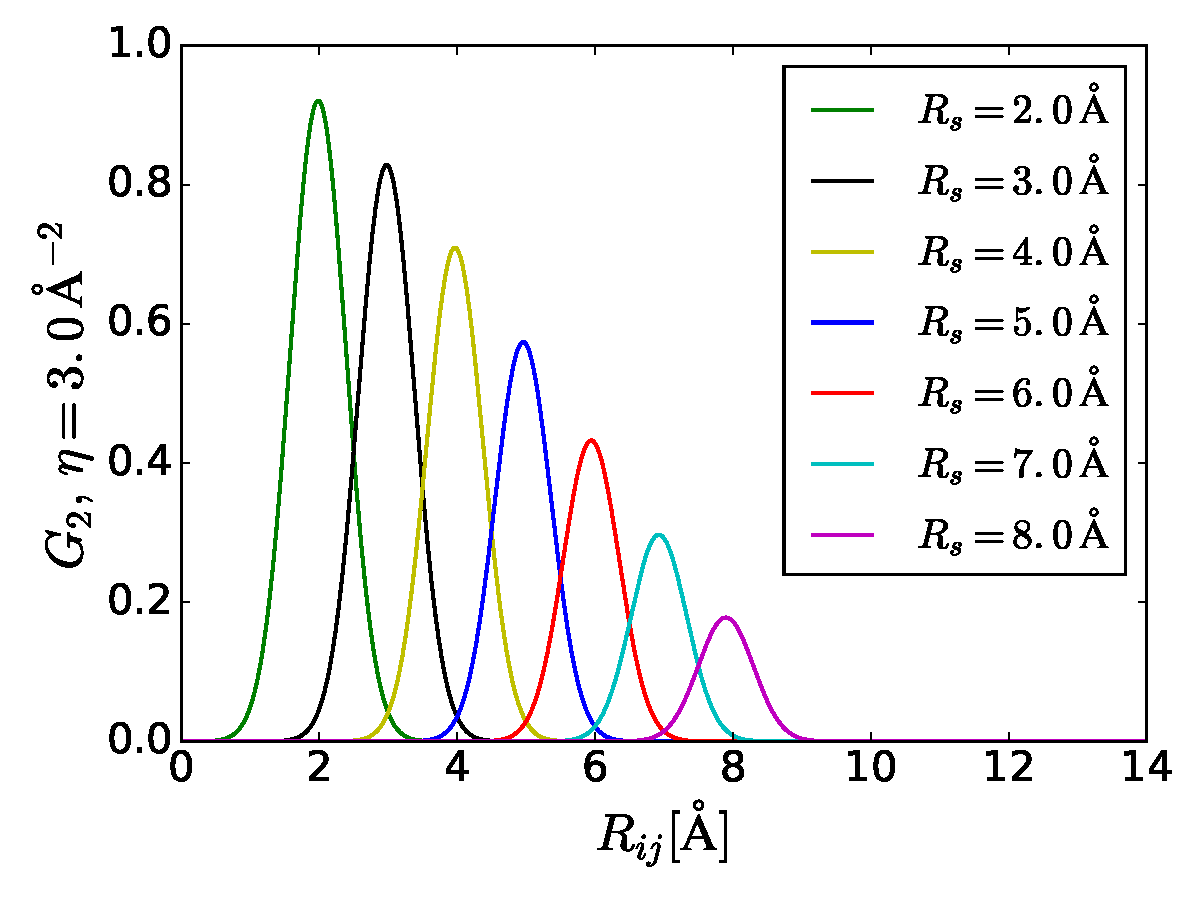
\includegraphics[width=\linewidth]{Figures/Theory/G2_2.pdf} 
    \label{fig:radialSymmetriFunctions:c} 
  \end{subfigure}%%
  \begin{subfigure}{0.5\linewidth}
    \centering
    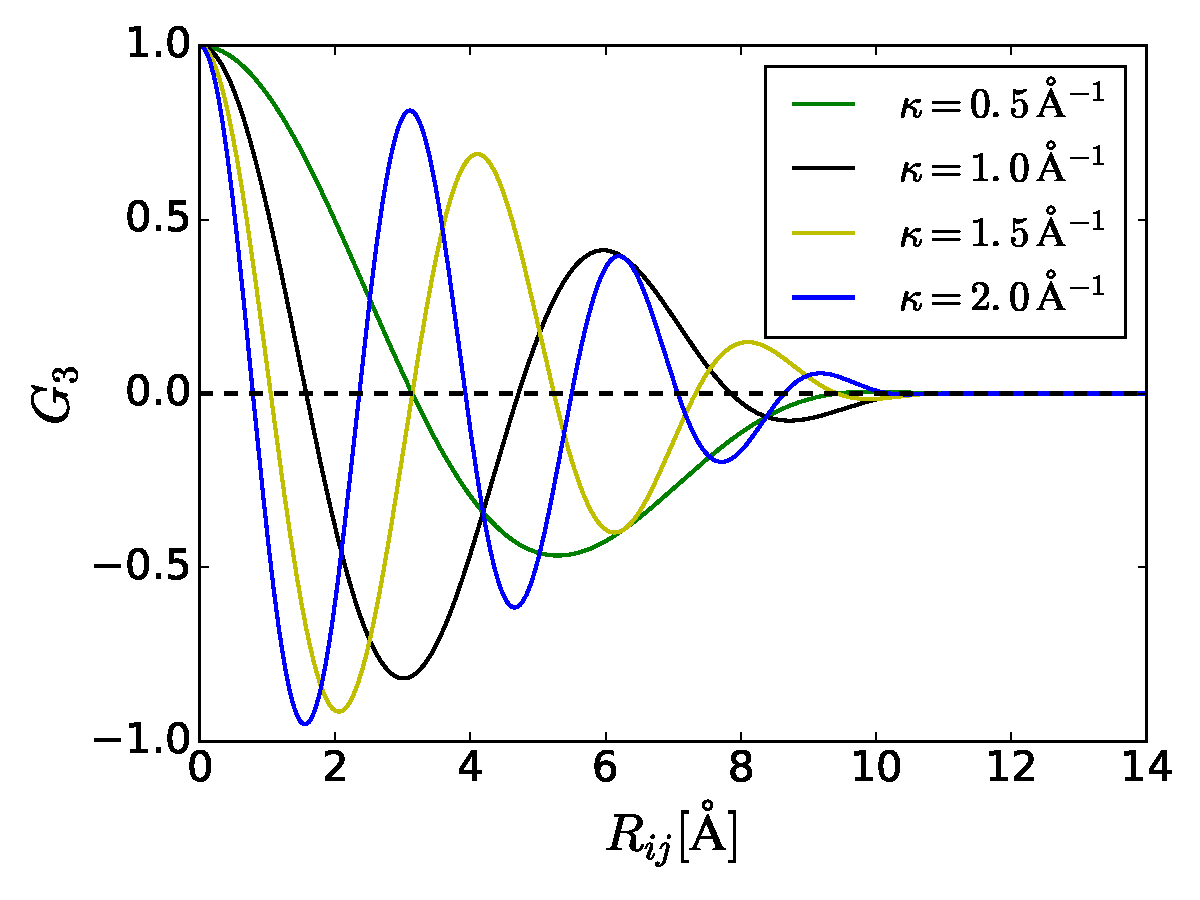
\includegraphics[width=\linewidth]{Figures/Theory/G3.pdf} 
    \label{fig:radialSymmetriFunctions:d} 
  \end{subfigure} 
  \vspace{-1.5ex}
  \caption{Radial symmetry functions $G^1$, $G^2$ and $G^3$ for an atom with one neighbour only. A set of such 
	   functions represents the radial distrubution of neighbours around a central atom placed at the origin.
	   For $G^2$ and $G^3$ a cutoff $r_c = \SI{11.0}{\angstrom}$ has been used. $r_{ij}$, $r_c$ and $r_s$ are in 
	   units of $\SI{}{\angstrom}$, while $\eta$ and $\kappa$ have units $\SI{}{\angstrom}^{-2}$ and 
	   $\SI{}{\angstrom}^{-1}$ respectively.}
  \label{fig:radialSymmetriFunctions} 
  \vspace{-1.5ex}
\end{figure}

\subsubsection{Angular symmetry functions}
To obtain a suitable structural fingerprint of the atomic environments, we also need the angular distribution
of neighbouring atoms. This can be achieved by using functions depending on $\theta_{jik}$, which
is the angle formed by the central atom $i$ and the two interatomic distances $r_{ij}$ and $r_{ik}$. 
The potential is periodic with respect to this angle, so we can use the cosine of $\theta_{jik}$ instead. 
We thus define an angular symmetry function as a sum over all cosines with respect to any possible triplet
($i$, $j$, $k$), multiplied by Gaussians of the three interatomic distances and the respective cutoff functions,
\begin{equation}
\begin{aligned}
 G_i^4 = 2^{1-\zeta}\sum_{j\neq i}\sum_{k>j} &\Big[(1 + \lambda \cos\theta_{jik})^\zeta \,
 \exp(-\eta (r_{ij}^2 + r_{ik}^2 + r_{jk}^2))  \\
 &f_c(r_{ij}) f_c(r_{ik}) f_c (r_{jk})\Big]
 \label{G4}
\end{aligned}
\end{equation}
This function is zeroed out if any of the interatomic distances is larger than $r_c$. The parameter $\eta$ takes here
into account that the angular contribution depends on the atomic seperations. The angular arrangement can be 
investigated by using different values for $\zeta$ while the normalization factor $2^{1-\zeta}$ ensures that the range of 
values is independent of the choice of $\zeta$. The parameter $\lambda \in {-1,1}$ can be used to invert the shape of the 
cosine function. For $\lambda = +1$ the maxima of the cosine terms are at $\theta_{jik} = 0^\circ$, 
while for $\lambda=-1$ they are located at $\theta_{jik} = 180^\circ$. The presence of the cutoff function $r_{jk}$
ensures that only triplets where all three inter-atomic distances are within the cutoff radius are included. 
Another function can be defined that has no constraint on $r_{jk}$,
\begin{equation}
  G_i^5 = 2^{1-\zeta}\sum_{j\neq i}\sum_{k>j} \Big[(1 + \lambda \cos\theta_{jik})^\zeta \,
 \exp(-\eta (r_{ij}^2 + r_{ik}^2)) \,
 &f_c(r_{ij}) f_c(r_{ik})\Big]
 \label{G5}
\end{equation}
which will generally lead to larger function values than \eqref{G4} because the lack of constraint on $r_{jk}$ results in 
a larger number of non-zero terms in the summation. The angular parts of $G_i^4$ and $G_i^5$ are identical, 
\begin{equation}
 G_i^\theta = 2^{1-\zeta}(1 + \lambda \cos\theta_{jik})^\zeta
\end{equation}
and is shown in \autoref{fig:angularSymmetryFunctions} for different values of $\zeta$. 
\begin{figure}
  \begin{subfigure}{0.5\linewidth}
    \centering
    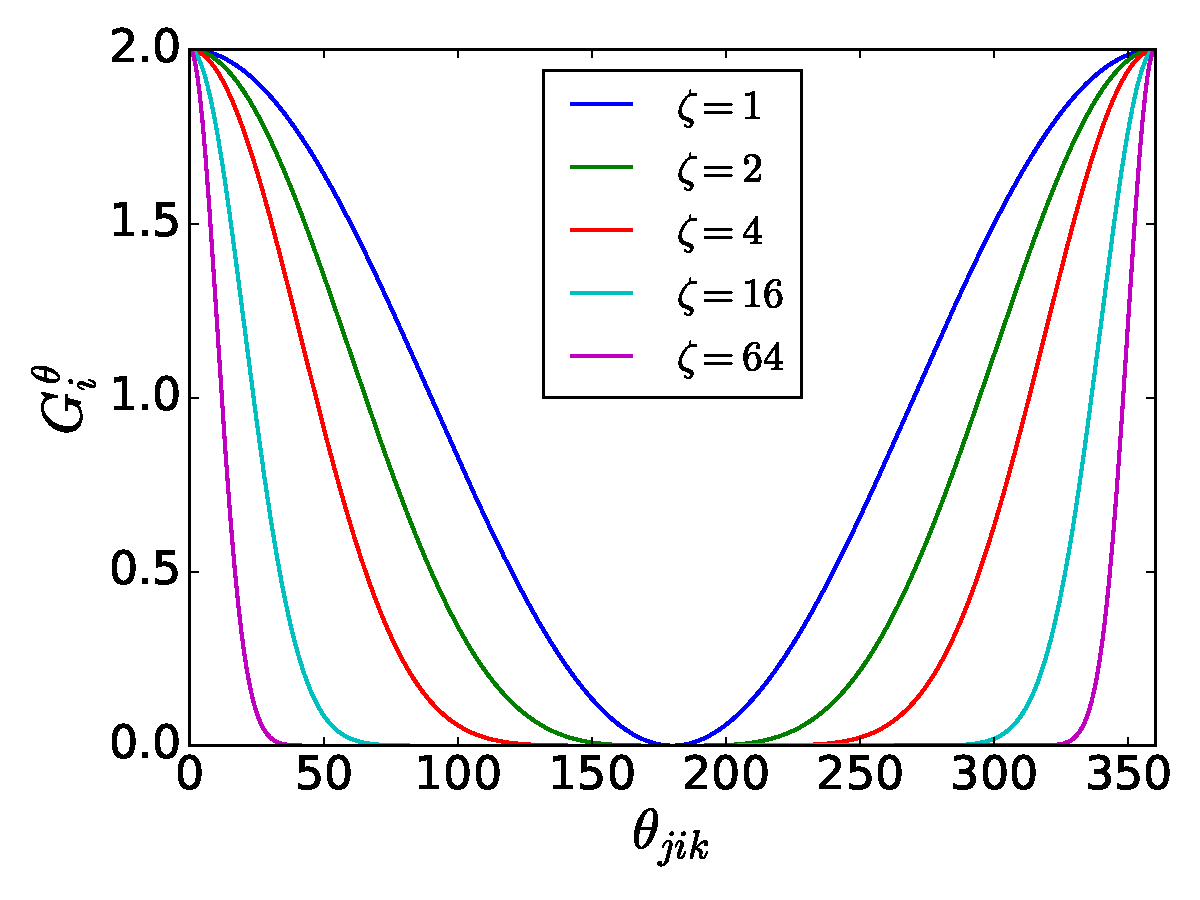
\includegraphics[width=\linewidth]{Figures/Theory/G4G5angular1.pdf}
    \subcaption{}
    \label{fig:angularSymmetryFunctions:a} 
  \end{subfigure}%% 
  \begin{subfigure}{0.5\linewidth}
    \centering
    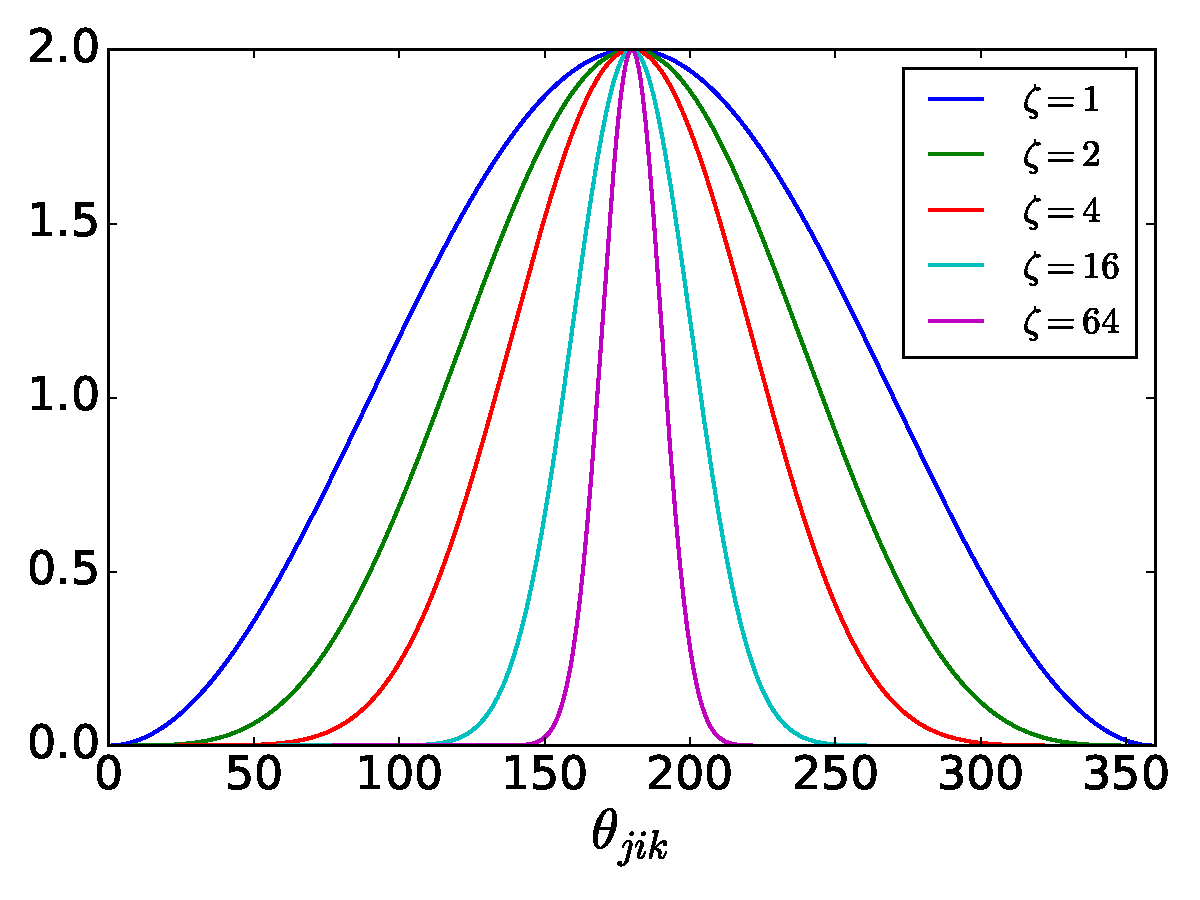
\includegraphics[width=\linewidth]{Figures/Theory/G4G5angular2.pdf} 
    \subcaption{}
    \label{fig:angularSymmetryFunctions:b} 
  \end{subfigure} 
  \caption{Angular part of symmetry functions $G_i^4$ and $G_i^5$ for an atom with one neighbour only. A set of such 
	   functions represents the angular distrubution of neighbours around a central atom placed at the origin.
	   $\lambda = +1$ for \autoref{fig:angularSymmetryFunctions:a}, $\lambda=-1$ for \autoref{fig:angularSymmetryFunctions:b}.}
 \label{fig:angularSymmetryFunctions} 
\end{figure}

\subsubsection{Determining the symmetry parameters}
The parameter values $r_c, \eta, r_s, \zeta$ and $\lambda$ are not automatically optimized, like the weights. 
They need to be pre-determined, and remain fixed during the training. In the context of machine learning, such variables are called
\textit{hyperparameters}, while the variables that are optimized during training are the \textit{model parameters}, i.e.\ 
the weights and biases. Other examples of hyperparameters are the learning rate (\autoref{sec:optimization}) and 
the number of NN nodes and layers. Various techniques for deciding on satisfactory hyperparameters are
discussed in  \autoref{sec:settingHyperParams}. 

They symmetry function set is
an integral part of the NN, and needs to be evaluated together with the NN itself when applied in simulations. 
The symmetry parameters must be customized for the system under cosideration; different strategies regarding this
is described in \autoref{sec:constructingSymmetry}.


\subsection{Symmetry functions and forces} \label{sec:symmAndForces}
To integrate Newton's laws in MD simulations we need the forces on all the atoms. The force field associated with a PES
was introduced in section \ref{sec:potentialEnergySurfaces} and is restated here for reference:
\begin{equation}
 \vec{F} = -\nabla E
 \label{forcePES2}
\end{equation}
In the present case, the total energy $E$ of the system is defined as a sum over all the atomic energies \eqref{systemEnergy}. 
Further, we have applied a cutoff so that each atom only gets energy contributions from its atomic environment up 
to a certain distance $r_c$.
The force component $F_{k,\alpha}$, $\alpha = (x,y,z)$ acting on atom $k$ with respect to coordinate $r_{k,\alpha}$,
can therefore be written \cite{Behler11symmetry}
\begin{equation}
 F_{k,\alpha} = -\frac{\partial E}{\partial r_{k,\alpha}} = -\sum_{i=1}^N\frac{\partial E_i}{\partial r_{k,\alpha}}
 = -\sum_{i=1}^{N_k+1}\frac{\partial E_i}{\partial r_{k,\alpha}}
 \label{forceAtomk}
\end{equation}
$N$ is as before the total number of atoms, while $N_k$ is the number of neighbours of atom $k$. 
Note that $E_k$ is included in the above sum - atom $k$ itself contributes to the total energy of its atomic
environment. We therefore have $N_k+1$ contributions. 

NNs have as we have seen well-defined functional forms, and analytic derivatives are therefore readily available.
However, when symmetry transformations is applied, there is only an indirect relation between the energy and the cartesian coordinates
of the atoms. To calculate the force \eqref{forceAtomk} we therefore need to apply the chain rule,
\begin{equation}
 F_{k,\alpha} = -\sum_{i=1}^{N_k+1}\frac{\partial E_i}{\partial r_{k,\alpha}} = 
 -\sum_{i=1}^{N_k+1}\sum_{s=1}^{M_i}\frac{\partial E_i}{\partial G_{i,s}}\frac{\partial G_{i,s}}{\partial r_{k,\alpha}}
 \label{forceAtomkChainRule}
\end{equation}
where $M_i$ is the number of symmetry functions of atom $i$. In other words, we need to sum over all the symmetry functions
of all the neighbours $i$ of atom $k$ and $k$ itself. This is the reverse process of \eqref{BPatomicEnergy},
\begin{equation}
 E_i \rightarrow F_\mathrm{e}[\vec{G}_\mathrm{e}(\vec{r}_{ij})] \rightarrow
 \vec{G}_\mathrm{e}(\vec{r}_{ij}) \rightarrow  \vec{r}_{ij}   
 \label{BPatomicForce}
\end{equation}
where the differentiation is perfomed in the direction of the arrows. 
We realize that the first term
$\partial E_i/\partial G_{i,s}$ is the derivative of the output of the atomic NN of atom $i$ with respect to the inputs,
i.e.\ the gradient of the NN. This is an analytic gradient
which is given by the architecture of the NN, including the values of the weights and biases.
We recall from \autoref{sec:backprop} that the backpropagation algorithm calculates the derivatives of all neurons in a NN to obtain
the amount of which each weight and bias should be adjusted during training. We can thus use a slightly modified version
of this algorithm to compute the gradient of a NN,
\begin{enumerate}
 \item Instead of backpropagating the derivative of the cost function, 
 we backpropagate the derivative of the output neuron itself.
 For output neurons with the identity activation function \eqref{outputActivation}, 
 this derivative is 1. 
 \item The derivative is propagated all the way back to the input nodes. During training, the propagation
 stops at the weights connecting the input layer and the first hidden layer. 
\end{enumerate}
This procedure clarifies how a fully-connected feed-forward NN is built: To get the derivative of the output neuron
w.r.t. the input neurons, we have to also compute the derivative of all the neurons in-between because
all nodes in each layer are connected to all nodes in the following layer. 

The second term $\partial G_{i,s}/\partial R_{k,\alpha}$ in \eqref{forceAtomkChainRule} is given by the 
definition of the employed symmetry functions. 
The derivatives of the Behler symmetry functions in \autoref{sec:symmetryFunctions} are 
listed in Appendix \autoref{app:appendixA1}.

\subsubsection{Change of coordinates}
In a MD simulation we only work with relative or inter-atomic coordinates and potentials. 
The training of neural networks is also based on an atom-centered approach; the cartesian coordinates
that is given as input to the symmetry functions are always atom-centered. This means that the atom
in question is placed at the origin and the positions of all neighbouring atoms are measured relative to 
the origin. Effectively, we are making a change of coordinates to the neighbours $j$ of the central atom $i$,
\begin{equation}
 \vec{r}_j \rightarrow \vec{r}_j - \vec{r}_i
 \label{changeOfCoordinates}
\end{equation}
This is in accordance with the Behler symmetry functions, which only operate with relative coordinates. 
It is however not trivial how this affects the above equations for the forces, which are not written in 
an atom-centered way. The process of obtaining the forces can be illustrated with an example system
consisting of three atoms of the same element with positions $\vec{r}_i$ where $i = 0,1,2$, shown in \autoref{fig:threeAtoms}.
\begin{figure}
\begin{center}
  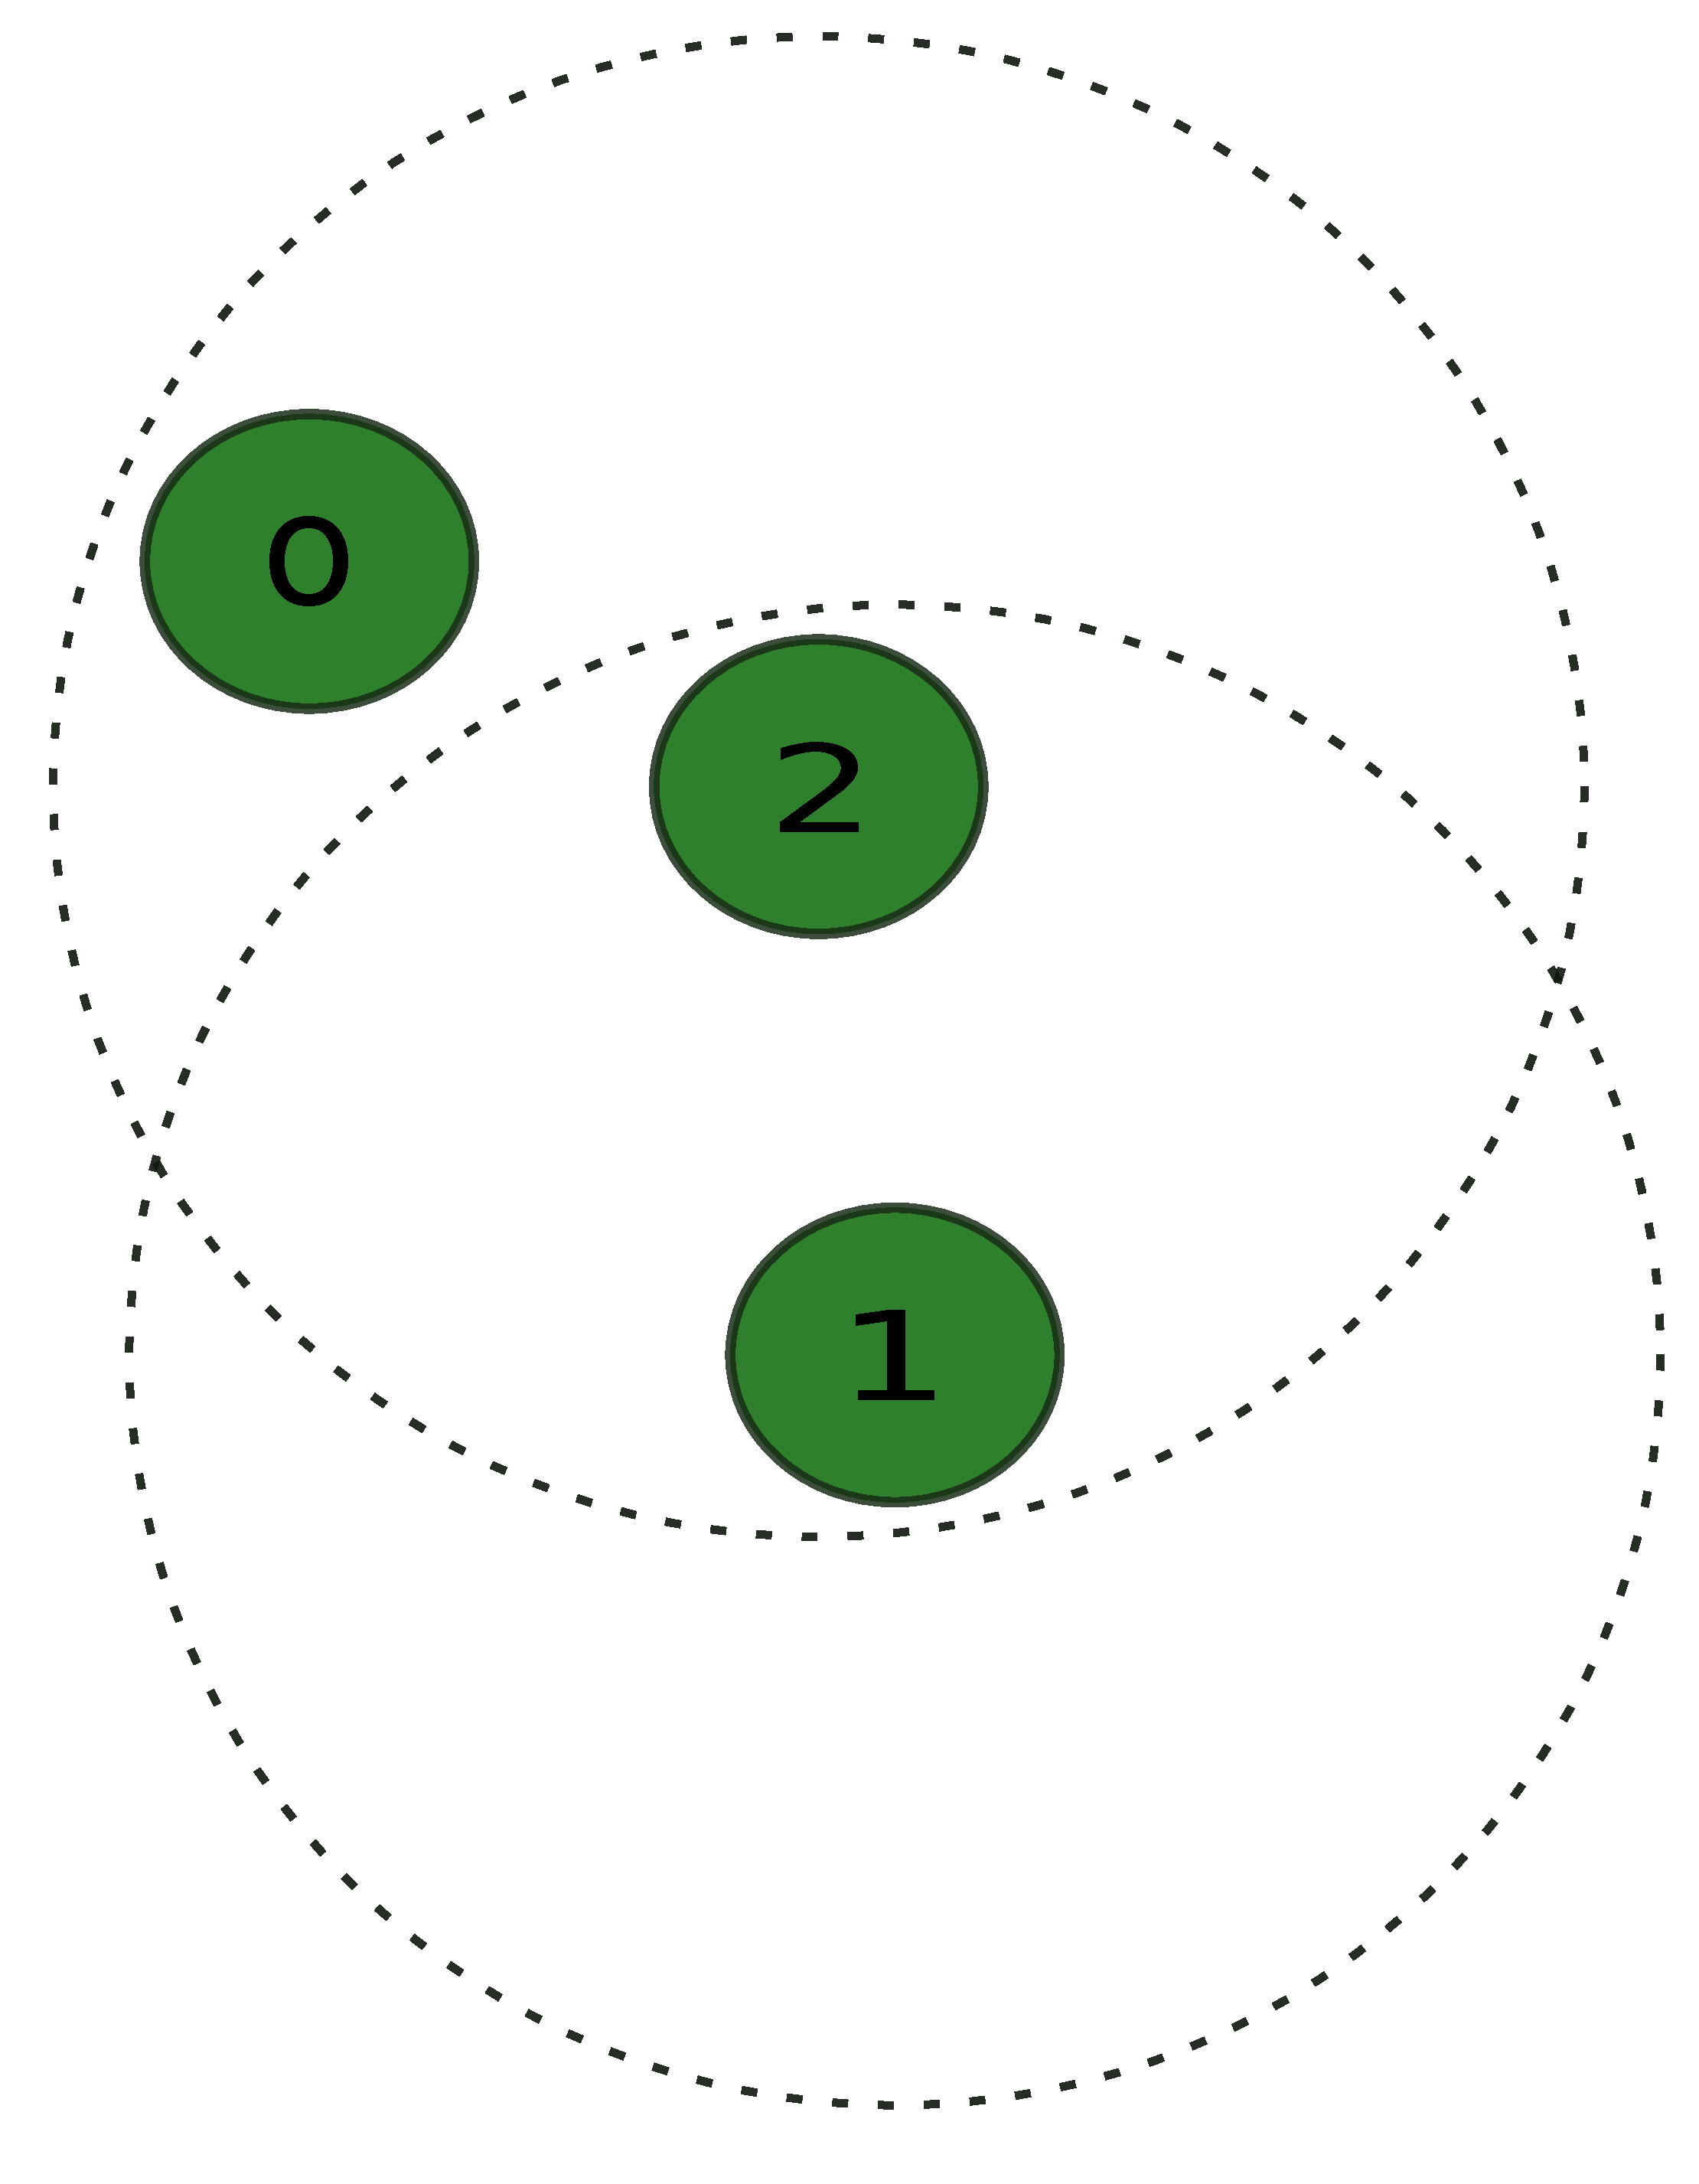
\includegraphics[width = 0.4\linewidth]{Figures/Implementation/3atoms.pdf}
  \caption{Example system of three atoms of the same type. Only atom 2 is inside the cutoff sphere of atom 1, thus we only need to 
	   take the energy of atom 1 and 2 into account to find the force on atom 1. Since the atoms are of the same type,
	   they have identical atomic NNs and symmetry function sets.}
  \label{fig:threeAtoms}
  \end{center}
\end{figure}
We want to find the force on atom 1 in the $x$-direction. Atom 0 is outside the cutoff sphere of atom 1, 
so according to \eqref{forceAtomk} the force is,
\begin{equation}
 F_{1,x} = \frac{\partial E_1}{\partial x_1} + \frac{\partial E_2}{\partial x_1}
 \label{forceOnAtom1}
\end{equation}
For simplicity, we assume that each atom only have two different symmetry functions describing their atomic environment;
one $G_{i,0}^2$ function describing the radial arrangement of neighbours and one $G_{i,1}^5$ dealing with the angular distribution.
Each atomic NN thus has two inputs and one output. 
Since the three atoms are all of the same type, they will have identical NNs $F$ and 
symmetry vectors $\vec{G} = (G_{i,0}^2, G_{i,1}^5)$. 
We will therefore denote the the two symmetry functions simply as $G_2$ and $G_5$. 
In the following we apply the notation $r_{ij} = |\vec{r}_j - \vec{r}_i|$. 
The expressions for $E_1$ and $E_2$ are,
\begin{equation}
 E_1 = F\bigr[G_2(r_{12})\bigr]
 \label{energyAtom1}
\end{equation}
$G_5$ is zero because atom 1 only has one neighbour. Further, 
\begin{equation}
 E_2 = F\bigr[G_2(r_{20}, r_{21}) + G_5(r_{20},r_{21},\theta_{021})\bigr]
 \label{energyAtom2}
\end{equation}
We note that atom 2 receives an energy contribution from both atom 0 and 1, so that 
its $G_2$ function is a sum containing two terms. 
To compute the derivatives of these energies with respect to the $x$-coordinate of atom 1, we
must take into account the change of coordinates \eqref{changeOfCoordinates}. We have that
\begin{equation}
 \frac{\partial G_2(x_{ij})}{\partial x_j} = \frac{\partial G_2(x_{ij})}{\partial x_{ij}}\frac{\partial x_{ij}}{\partial x_j}
 = \frac{\partial G_2(x_{ij})}{\partial x_{ij}}\frac{\partial (x_j-x_i)}{\partial x_j} = 
 \frac{\partial G_2(x_{ij})}{\partial x_{ij}}
 \label{changeOfCoordsSymmetry1}
\end{equation}
and
\begin{equation}
 \frac{\partial G_2(x_{ij})}{\partial x_i} = \frac{\partial G_2(x_{ij})}{\partial x_{ij}}\frac{\partial (x_j-x_i)}{\partial x_i} =
 -\frac{\partial G_2(x_{ij})}{\partial x_{ij}}
 \label{changeOfCoordsSymmetry2}
\end{equation}
which is also valid for the other radial symmetry functions $G_1$ and $G_3$.   
This symmetry, which is a manifestation of Newton's third law,
enable us to calculate the derivatives in \eqref{forceOnAtom1}. For radial symmetry functions
dependent on several atom pairs, \eqref{changeOfCoordsSymmetry1} and \eqref{changeOfCoordsSymmetry2} 
apply to each term in the sum seperately. Further, the symmetry is also present for each atom in a triplet,
\begin{equation}
 \frac{\partial G_5(x_{ij}, x_{ik}, \theta_{jik})}{\partial x_i} = 
 -\frac{\partial G_5(x_{ij}, x_{ik}, \theta_{jik})}{\partial x_{ij}} - 
 \frac{\partial G_5(x_{ij}, x_{ik}, \theta_{jik})}{\partial x_{ik}}
 \label{changeOfCoords3body1}
\end{equation}
and 
\begin{subequations}
\begin{align}
 \frac{\partial G_5(x_{ij}, x_{ik}, \theta_{jik})}{\partial x_j} &= 
 \frac{\partial G_5(x_{ij}, x_{ik}, \theta_{jik})}{\partial x_{ij}}
 \label{changeOfCoords3body2} \\
 \frac{\partial G_5(x_{ij}, x_{ik}, \theta_{jik})}{\partial x_k} &= 
 \frac{\partial G_5(x_{ij}, x_{ik}, \theta_{jik})}{\partial x_{ik}}
 \label{changeOfCoords3body3}
\end{align}
\end{subequations}
i.e.\ the derivative w.r.t. $i$ is the negative sum of the derivatives w.r.t. $j$ and $k$. This is a symmetry we
have exploited in our code, see \autoref{sec:extendingLammps}. 

To obtain the derivatives of the energies \eqref{energyAtom1} and \eqref{energyAtom2}, we apply the chain rule
\begin{equation}
 \frac{\partial E_1}{\partial x_1} = \frac{\partial F}{\partial G_2(r_{12})}
 \frac{\partial G_2(r_{12})}{\partial x_1} = 
 -\frac{\partial F}{\partial G_2(r_{12})}\frac{\partial G_2(r_{12})}{\partial x_{12}}
\end{equation}
where we have applied the above change of coordinates \eqref{changeOfCoordsSymmetry2}.
Using \eqref{changeOfCoordsSymmetry1}, the derivative of $E_2$ can be calculated correspondingly,
\begin{subequations}
\begin{align}
 \frac{\partial E_2}{\partial x_1} &= 
 \frac{\partial F}{\partial G_2(r_{20}, r_{21})}\frac{\partial G_2(r_{20}, r_{21})}{\partial x_1} + 
 \frac{\partial F}{\partial G_5(r_{20},r_{21},\theta_{021})}\frac{G_5(r_{20},r_{21},\theta_{021})}{\partial x_1} \\
 &= \frac{\partial F}{\partial G_2(r_{21})}\frac{\partial G_2(r_{21})}{\partial x_{21}} + 
 \frac{\partial F}{\partial G_5(r_{20},r_{21},\theta_{021})}\frac{G_5(r_{20},r_{21},\theta_{021})}{\partial x_{21}}
\end{align}
\end{subequations} 
From the definition of $G_2$ \eqref{G2} we see that the sum contains two terms
in the case of atom 2, one for each pair interaction between atom 2 and its two neighbours. 
The interaction term between atom 0 and 2
cancels when differentiated with respect to the coordinates of atom 1, and is thus not included in the force on atom 1. 
 
The sum in $G_5$ \eqref{G5} however, consists of only one term corresponding to the only unique triplet with atom 2
as the central atom. This term is directly dependent on the coordinates of atom 0, which means that 
an atom which is outside the cutoff sphere of atom 1 still contributes to the force. This is an artefact of many-body potentials
like the NNPs employed in this thesis: The force acting on an atom $i$ depends on the positions of the atoms as 
far as $2r_c$ away because \textit{neighbours of neighbours} are included in the
energies that are differentiated to obtain the force. 
This large effective range of atomic interactions is however not of great importance, taking into account
that the interaction strength falls rapidly with distance for most systems where Coulomb forces are not included. 


\section{Summary}
In this chapter we have introduced the Behler-Parrinello method for constructing NNPs to be used in MD simulations. 
This scheme employs certain symmetry functions that have the following desirable properties,
\begin{enumerate}
 \item They are atom-centered and have an inherent cutoff $r_c$ that defines a chemical environment of tractable size. 
 \item They yield the same number of outputs independent of the number of inputs. 
 \item The order of the inputs is irrelevant. 
 \item They are invariant with respect to translation and rotation.
 \item They have analytic derivatives.
\end{enumerate}
1. and 2. solves the technical issues of the limited and fixed dimensionality of MLPs respectively.
3. and 4. deals with physical symmetries, namely that the energy of an atomic system does not change
if two identical atoms are exhanged, or if the system undergoes a translation or a rotation. 
5. is a wanted property because the symmetry functions are differentiated to obtain forces. 

In \autoref{sec:constructingNNP} we present the complete workflow for constructing a NNP, 
including a description of how to assemble a symmetry function set, found in 
\autoref{sec:constructingSymmetry}.




\part{Implementation and results}

\chapter{LAMMPS} \label{sec:lammps}
LAMMPS (Large-scale Atomic/Molecular Massively Parallel Simulator)
is a classical molecular dynamics simulation package 
developed at Sandia National Laboratories \cite{Plimpton95}. It is written
in highly portable and extendable objected-oriented C\texttt{++}. 
The package contains functionality encompassing a wide variety of 
potentials, atom types, thermostats and 
ensembles, and is able to simulate a large number
of different systems, including atoms, molecules, 
coarse-grained particles, polymers, graunular materials
and metals. LAMMPS can be run on a single processor
or in parallell. 

There exist several other molecular dynamics packages, 
like GROMACS, OpenMD, Aber and NAMD that could also
have served the purpose of this thesis. We have chosen
to work with LAMMPS because it is well documented% 
\footnote{\href{http://lammps.sandia.gov/doc/Manual.html}{lammps.sandia.gov/doc/Manual.html}},
easy to expand upon%
\footnote{\href{http://lammps.sandia.gov/doc/Developer.pdf}{lammps.sandia.gov/doc/Developer.pdf}},
and because the Computational
physics group at UiO has a lot of experience with using
it for molecular dynamics simulations. 

In this chapter we will outline the basic usage of LAMMPS, including
a walkthrough of an example input script. We also describe its
class hierarchy and how we can add our own functionality
to the package.

\section{Installing LAMMPS}
We have chosen to install LAMMPS by cloning
the Github repository and compile the source
code by running \texttt{make} in the source directory. 
To compile a serial version of the software, we simply run
the command
\begin{lstlisting}[language=bash]
 make serial
\end{lstlisting}
while the corresponding command for the parallel
MPI version is
\begin{lstlisting}[language=bash]
 make mpi
\end{lstlisting}
New updates can be downloaded by setting an
upstream git remote to point to the LAMMPS
GitHub repository and doing a \texttt{git fetch upstream}. 
LAMMPS also have several additional packages that
can be installed. This can be done by running
\begin{lstlisting}[language=bash]
 make yes-<package name>
\end{lstlisting}
e.g.\ \texttt{manybody} to install many-body potentials
like Stillinger-Weber and Vashishta. 

\section{LAMMPS input script} \label{sec:lammpsInputScript}
LAMMPS is run by providing an input script as 
argument to the excecutable. This input script
is read line by line and has its own syntax. 
A good way to show the basics an input file
is to look at a simple example. 
We have chosen to have a look at a script
to measure the radial distribution function of a Si crystal with the Stillinger Weber (SW) potential (\autoref{sec:stillingerWeber}),
\begin{lstlisting}[style=lammps]
# initialization
units 			metal		
dimension 		3
boundary		p p p		
atom_style		atomic		

# create geometry and atoms
lattice 		diamond 5.431
variable		L equal 10
region 			simBox block 0 ${L} 0 ${L} 0 ${L}
create_box		1 simBox
create_atoms	1 box

# set mass and initial temperature
mass			1 28.06
variable		temp equal 300
velocity		all create ${temp} 87287

# compute radial distribution function
compute 		radialDist all rdf 100

# potential 
pair_style		sw
pair_coeff		* * Si.sw Si
neighbor		0.5 bin
neigh_modify	every 20 delay 0 check no

# integration
timestep 		0.01
run_style 		verlet
fix 			integration all nve

# output
thermo			50
thermo_style 	custom step temp density press ke pe etotal 
thermo_modify 	norm yes

# thermalize before sampling rdf
run				10000
fix radial all ave/time 100 10 1000 c_radialDist[*] file &
    rdf.txt mode vector
run				10000
\end{lstlisting}
We will in the following briefly explain what
processes that are evoked in LAMMPS when the 
above commands are read. We start with the initialization of 
three basic properties of the simulation: Units, boundary conditions and particle types.
\begin{lstlisting}[style=lammps]
 units 		metal
\end{lstlisting}
This command defines the units that are used 
in the simulation and the output. LAMMPS have eight
different unit sets. The \texttt{metal} set measures
distance in \AA{}ngstr\o{}m, energy in eV and temperature
in Kelvin. The choice of units depends on the system
that is investigated and the scale we are looking at.
\begin{lstlisting}[style=lammps]
 boundary 	p p p
\end{lstlisting}
We wish to measure the radial distribution function in a \textit{bulk}
Si crystal, thus we want to have periodic 
boundary conditions in all three dimensions, 
annotated by a \texttt{p}. LAMMPS can also handle stiff \texttt{f}
and adaptive \texttt{s} non-periodic boundaries. Adaptive
means that the position of the face is set so as to
encompass the atoms in that dimension. 
\begin{lstlisting}[style=lammps]
 atom_style atomic
\end{lstlisting}
Different systems need different information
to be stored for each atom. For style \texttt{atomic}, only
the default attributes are associated with each atom, 
namely coordinates, velocities, atom IDs and types. 
This is sufficient for non-bonded potentials like Stillinger-Weber.

\noindent Next, we create the geometry of the simulation domain.
\begin{lstlisting}[style=lammps]
lattice 	diamond 5.431
\end{lstlisting}
This defines the initial configuration of the atoms. 
Here, a diamond cubic lattice with a lattice constant of
5.431 is used, which is the crystal structure of Si. Other types of lattices based on
cubic or square unit cells are also available. 
\begin{lstlisting}[style=lammps]
variable	L equal 10
region 		simBox block 0 ${L} 0 ${L} 0 ${L}
\end{lstlisting}
The geometry of the system is defined with the \texttt{region}
command. The \texttt{block} style is simply a 3-dimensional
straight-faced box with a size of $L = 10$ unit
cells in each dimension. We have labelled the 
region \texttt{simBox}. 
The number of unit cells
\texttt{L} is defined as a LAMMPS \texttt{variable}. Variables
can be referenced elsewhere in the script by
writing \texttt{\$\{variable\_name\}} to become part of a new input
command like above. LAMMPS enables many styles
of variables to be defined. 
\begin{lstlisting}[style=lammps]
create_box		1 simBox
create_atoms	1 box
\end{lstlisting}
The command \texttt{create\_box} creates a simulation box 
based on the specified region, in our case the 
\texttt{block} region defined above. The argument specifies
the number of atom types that will be used in the
simulation. Next, \texttt{create\_atoms} with the argument
\texttt{box} fills the simulation
domain with atoms of type 1 on the lattice. 
LAMMPS also lets you create a random collection
of atoms or single atoms at specified coordinates.
\begin{lstlisting}[style=lammps]
mass			1 28.06
variable		temp equal 300
velocity		all create ${temp} 87287 
\end{lstlisting}
We need to assign mass to the atoms. For \texttt{metal} units, 
mass is measured in grams/mole. The atoms are also
given an initial velocity that corresponds to 
the given initial temperature. 
\begin{lstlisting}[style=lammps]
pair_style		sw
pair_coeff		* * Si.sw Si
\end{lstlisting}
The choice of potential is made with the 
\texttt{pair\_style} command. We want to simulate
interactions using the Stillinger-Weber potential \texttt{sw}. The SW parameters
are set with \texttt{pair\_coeff}, where \texttt{Si.sw} is a text file from which all parameters are read.  
Further, asterisks signifies that the potential file contains parameters for all elements, in this case for 
Si only. 
\begin{lstlisting}[style=lammps]
neighbor		0.5 bin
neigh_modify	every 20 check yes
\end{lstlisting}
These commands sets parameters that affect the 
building of neighbor lists. The first argument
to \texttt{neighbor} is the skin size, while the 
second selects what algorithm is used
to build the lists. The \texttt{bin} style creates 
the lists by binning, which in most cases
(including ours) is the fastest method. 
Further, we can control how often the lists
are built with \texttt{neigh\_modify}. The above arguments
specifies that new neighbour lists are built 
every 20 steps, but every step LAMMPS checks
if any atom has moved more than half the skin distance.
If that is the case, new lists are built. 
\begin{lstlisting}[style=lammps]
timestep 		0.01
run_style 		verlet
fix 			integration all nve
\end{lstlisting}
LAMMPS integrates Newtons' equations of motion
with the velocity-Verlet algorithm by defualt. 
This is the integrator of choice for most MD
applications due to its simplicity and 
symplectic nature (\autoref{sec:timeIntegration}). The 
rRESPA integrator \cite{Tuckerman92} scheme is also available.
LAMMPS does however not integrate and update
the positions and velocities of the particles
if not explicitly told so. This is done with
a \texttt{fix}, which is any operation that is applied to the 
system during timestepping. The above \texttt{fix} 
tells LAMMPS to integrate all atoms in the system 
so that they follow trajectories consistent with 
the microcanonical ensemble. 
\begin{lstlisting}[style=lammps]
thermo			50
thermo_style 	custom step temp press ke pe etotal 
thermo_modify 	norm yes
\end{lstlisting}
We can control what thermodynamic properties 
to calculate and output with \texttt{thermo\_style}, while 
\texttt{thermo} decides how often they should be computed. 
We want to output the time step, temperature, 
pressure, kinetic energy, potential energy and total
energy. Also, we want to normalize the extensive
quantities (the energies) by the number of atoms. 
\begin{lstlisting}[style=lammps]
compute 		radialDist all rdf 100
fix radial all ave/time 100 10 1000 c_radialDist[*] file &
    rdf.txt mode vector
\end{lstlisting}
The radial distribution function are measured with a LAMMPS \texttt{compute}, 
which defines a computation that is perfomed on a group of atoms, in this case \texttt{all} atoms. 
For the \texttt{compute} to actually be executed, it needs
to be evoked by other LAMMPS commands, in this case the fix \texttt{ave\slash time}. 
The three numerical arguments specify how the distribution is averaged over time. 
Note that the \texttt{compute} is referenced by \texttt{c\_} followed by its label. 
\begin{lstlisting}[style=lammps]
run		5000
\end{lstlisting}
Lastly, we run the simulation for 5000 timesteps. 
LAMMPS allowes several run commands to be issued
after one another. This comes in handy if we want
to thermalize the system before measuring thermodynamic quantities,
\begin{lstlisting}[style=lammps]
 run 	5000
 fix radial all ave/time 100 10 1000 c_radialDist[*] file &
    rdf.txt mode vector
 run 	10000
\end{lstlisting}
When parsing the second run command, LAMMPS will
continue the dynamics while computing eventual
new fixes, computes, dumps etc.\ defined since
the last run command. 

This section has illuminated some of the basic
funcionality of LAMMPS through several comments
on a simple input script. Now we move on to
how class hierarchy of LAMMPS is structured. 

\section{LAMMPS structure}
LAMMPS is written in C\texttt{++} in an object-oriented
fashion. The class hierarchy is shown schematically
in \autoref{fig:lammpsClasses}. 
The top-level classes (blue)
are visible anywhere in LAMMPS.
Some selected sub-classes (green and yellow) are displayed. We recognize many 
of the input script commands among these sub-classes; a rule of thumb is that every input script
command has a corresponding class and a
corresponding file name in the source directory. 
For instance, we observe that the Stillinger-Weber potential ''PairSW'' is a sub-class of Pair.  
This potential was evoked by the command
\texttt{pair\_style sw} above and the source files are named
\texttt{pair\_sw.cpp} and \texttt{pair\_sw.h}. 
\begin{figure}
 \centering
 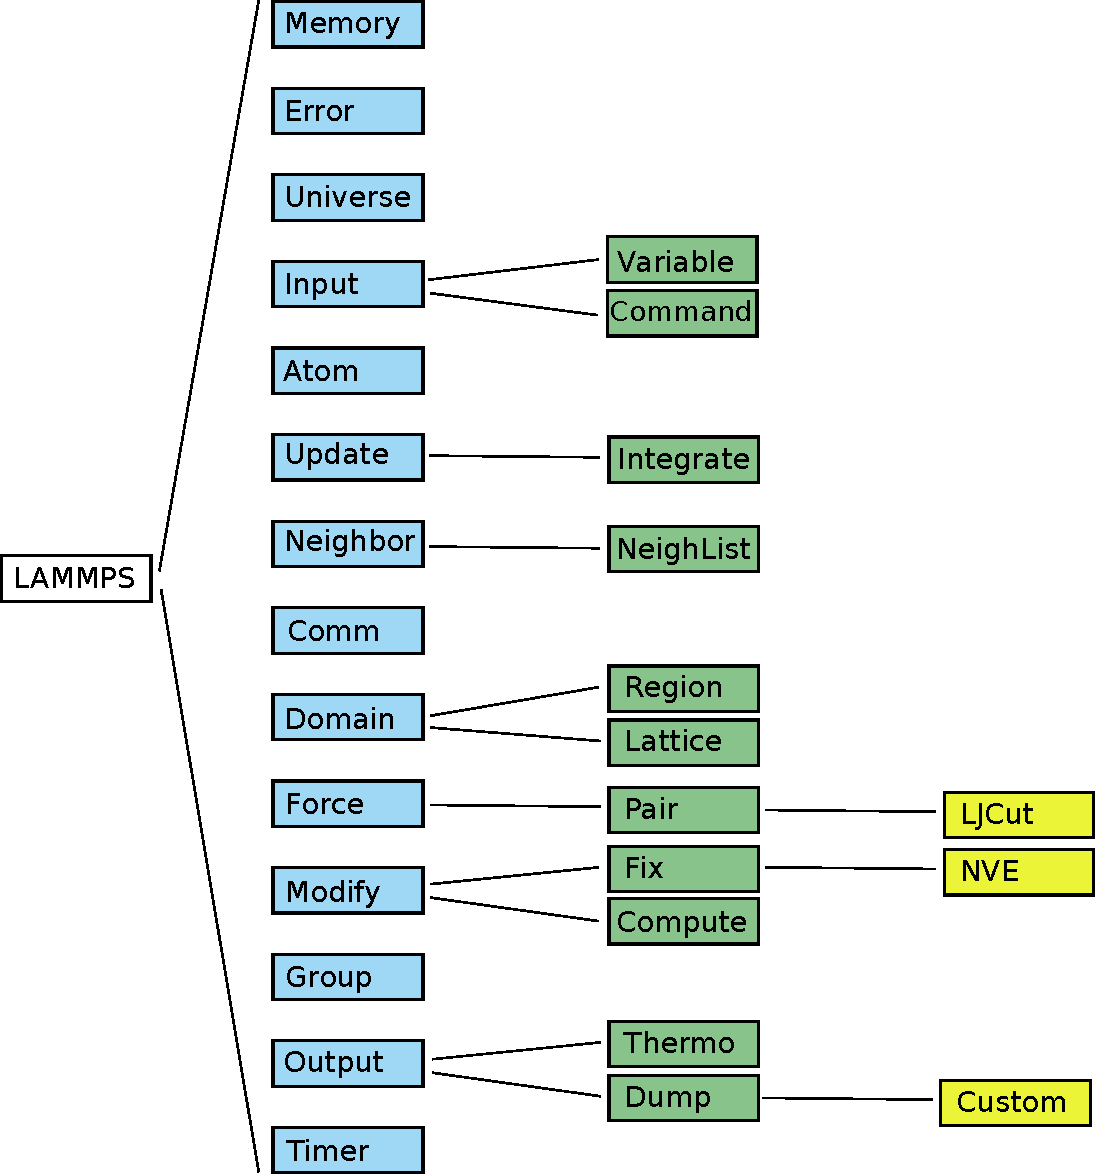
\includegraphics[width = 0.8\linewidth]{Figures/Implementation/lammpsClasses.pdf}
  \caption{Class hierarchy of LAMMPS. The inheritance is from left to right. 
	   The top-level classes (blue) are visible everywhere in the code. Only a selected set 
	   of sub-classes (green and yellow) is displayed, where we recognize many of the input script
	   commands.}
  \label{fig:lammpsClasses}
\end{figure}

We will not go into detail about the functionality
and communication of these classes. The one
that is the most relevant for this work is the \texttt{Pair} class. 
This is the parent class of non-bonded potentials, which
in LAMMPS includes many-body potentials like Stillinger-Weber and 
Vashishta. The NN potential in this thesis falls 
under this category, and thus inherits from \texttt{Pair}. 
In the following section we will describe how 
LAMMPS can be extended with such a new \texttt{pair\_style}.

\section{Extending LAMMPS} \label{sec:extendingLammps}
To extend LAMMPS with a new component, we 
simply add a new \texttt{*.cpp} and \texttt{*.h} file to the 
source directory and re-compile. The new class
will (in theory) work with all other LAMMPS 
classes without breaking any functionality. 
A good strategy is to start with an existing potential
source file that is somewhat similar to the one 
we want to make, instead of programming from scratch.
We aim to construct a many-body non-bonded neural network potential (NNP), and 
have chosen to base our implementation on the 
Stillinger-Weber source files.

\subsection{Potential initialization}
The new potential class is added to LAMMPS with the following function call in the header file,
\begin{lstlisting}[language=c++]
 PairStyle(nn/manybody,PairNNManyBody)
\end{lstlisting}
The first argument is the name the potential will have in the input script, while 
the second is the name of the class. 
To use our new NN potential in a simulation we simply write,
\begin{lstlisting}[style=lammps]
 pair_style 	nn/manybody
\end{lstlisting}
in the input script. This command evokes two functions in the source files that need to be implemented: \texttt{settings}
and \texttt{init\_style}. The former controls the number of arguments to 
\texttt{pair\_style}, which in our case is zero, 
\begin{minted}{C++}
void PairNNManyBody::settings(int narg, char **arg) {
  if (narg != 0) error->all(FLERR,"Illegal pair_style command");
}
\end{minted}
while the latter decides what kind of neighbour lists LAMMPS should provide to the potential, 
\begin{minted}{C++}
void PairNNAngular2::init_style() {
  // ... 
  if (force->newton_pair == 0)
    error->all(FLERR,"Pair style NN requires newton pair on");

  // need a full neighbor list
  int irequest = neighbor->request(this);
  neighbor->requests[irequest]->half = 0;
  neighbor->requests[irequest]->full = 1;
}
\end{minted}
Our NN potential needs full neighbour lists to be able to compute three-body terms. Further, 
we ensure that \texttt{newton\_pair} is set to 1, which tells LAMMPS to communicate forces attributed to ghost 
atoms to the original atoms. 

The parent class \texttt{Pair} has three \textit{pure virtual member functions}, i.e.\ functions that are required
to be implemented by a derived class: \texttt{compute}, \texttt{coeff} and the aforementioned \texttt{settings}. 
The \texttt{compute} method is where the forces and energies are calculated. This function is called
once each time step by the Verlet algorithm and the resulting forces are used to integrate Newton's equations
of motion. 

The coefficients of the employed potential are set in \texttt{coeff}, which in the case of a NN potential
is the weights, biases, symmetry function parameters and other hyperparameters. 
These are read from file, and based on information on the architecture of the NN, 
the network is reconstructed as a set of matrices and 
vectors, according to the description in \autoref{sec:MLPmodel}. This is achieved with the input script command,
\begin{lstlisting}[style=lammps]
 pair_coeff		* * <path-to-saved-NN> <cutoff> 
\end{lstlisting}
where the wildcard asterisks signify that the coefficients span all atom types and are read from file. 
If there are more than one element, a seperate NN file is read for each one. 
An example is $\mathrm{SiO}_2$,
\begin{lstlisting}[style=lammps]
 pair_coeff 	* * <path-1> <path-2> Si O <cutoff>
\end{lstlisting}


\subsection{Computing energies and forces}
Now that the NNP is set up, we are ready to employ it in simulations. 
The process of computing energies and forces with the NNP is described as follows,
\begin{enumerate}
 \item Initialize various variables like the vector of atom coordinates and the neighbour lists of each atom.
 \item Loop through all atoms. For each atom $i$:
 \begin{enumerate}
  \item Construct the input vector to the NN by evaluating the symmetry functions for all 
        atomic pairs and triplets below the cutoff radius. 
	The coordinates, types, angles etc.\ of all pairs and triplets must be stored for later force calculations. 
  \item Evaluate the NN corresponding to the element of atom $i$ to obtain its total potential energy.
  \item Calculate the gradient of the energy w.r.t. the symmetry function values by backpropagation.
  \item Differentiate the symmetry functions w.r.t. to the coordinates of all neighbours to obtain the total force on atom $i$.
 \end{enumerate}
\end{enumerate}
This process determines the structure of the \texttt{nn/manybody} \texttt{compute} function. 
We start out by accessing various variables needed to compute the forces,
\begin{minted}{c++}
double **x = atom->x;      // atom coordinates
double **f = atom->f;      // forces
int *type = atom->type;    // type of each atom	
int nlocal = atom->nlocal; // no. of atoms belonging to current processor  

int inum = list->inum;     // length of list containing all neighbour lists
int *ilist = list->ilist;  // local indicies of all local atoms
int *numneigh = list->numneigh; // lengths of each neighbour list
int **firstneigh = list->firstneigh; // all neighbour lists
\end{minted}
Next, we loop through all atoms in \texttt{ilist}. For each atom, we evaluate 
the two-body and three-body symmetry functions with the symmetry parameters read from file. 
We also store certain information on all neighbours. 
\begin{minted}{c++}
for (int ii = 0; ii < inum; ii++) {
  int i = ilist[ii];
  int itype = map[type[i]];

  double xtmp = x[i][0];
  double ytmp = x[i][1];
  double ztmp = x[i][2];

  // neighbour list of atom i
  int *jlist = firstneigh[i];
  int jnum = numneigh[i];
  
  // collect all pairs
  for (int jj = 0; jj < jnum; jj++) {
    int j = jlist[jj];
    j &= NEIGHMASK;
    tagint jtag = tag[j];
    int jtype = map[type[j]];

    double delxj = x[j][0] - xtmp;
    double delyj = x[j][1] - ytmp;
    double delzj = x[j][2] - ztmp;
    double rsq1 = delxj*delxj + delyj*delyj + delzj*delzj;

    if (rsq1 >= cutoffSquared) continue;   
    double rij = sqrt(rsq1);
    
    // store relative coordinates (delxj, delyj, delzj), distance rij, 
    // index j and type jtype. Initialize input vector. 
    
    // apply two-body symmetry
    for (int s=0; s < m_numberOfSymmFunc; s++)
      if ( m_parameters[s].size() == 3 )
          inputVector(0,s) += G2(rij, m_parameters[s][0],
                                 m_parameters[s][1], m_parameters[s][2]);
    
    // collect all triplets
    for (int kk = jj+1; kk < jnum; kk++) {
      // apply three-body symmetry and 
      // store configurations of all triplets...
\end{minted}
We are now ready to evalute the NN with the input vector of symmetry values. 
The NN is implemented as a function, shown here in the monatomic case for brevity,
\begin{minted}{c++}
double PairNNManyBody::network(arma::mat inputVector) {

  // no activation for input layer
  m_preActivations[0] = inputVector;
  m_activations[0] = m_preActivations[0];

  // hidden layers
  for (int i=0; i < nLayers; i++) {
    m_preActivations[i+1] = m_activations[i]*m_weights[i] + m_biases[i];
    m_activations[i+1] = sigmoid(m_preActivations[i+1]);
  }

  // identity activation for output layer
  m_preActivations[nLayers+1] = m_activations[nLayers]*m_weights[nLayers] + 
				m_biases[nLayers];
  m_activations[nLayers+1] = m_preActivations[nLayers+1];

  // return activation of single output neuron
  return m_activations[nLayers+1](0,0);
}
\end{minted}
where \texttt{sigmoid(A)} is a function that returns the sigmoid \eqref{sigmoidActivationFunction} 
of each element of a matrix \texttt{A}. 
Each variable with the \texttt{m\_} prefix is an \texttt{std::vector} containing a set of Armadillo matrices. 
For instance, \texttt{m\_weights[0]} is a matrix of all weights connecting the input layer 
and the first hidden layer. This results in highly readable code that is very similar to the mathematical 
description \eqref{forwardPropMatrix} %
\footnote{The weight-activation multiplication is in reverse order in the code because we use row vectors instead of column vectors.
Also, the indexing of the weight and bias vectors are different than in \eqref{forwardPropMatrixLammpsChapter}, as 
the activation and preactivation vectors also include the input layer. This also applies to the implementation
of backpropagation.},
\begin{equation}
 \begin{aligned}
  \vec{u}_l &= \mathrm{W}_l\vec{y}_{l-1} + \vec{b}_l \\
  \vec{y}_l &= f_l(\vec{u}_l)
  \label{forwardPropMatrixLammpsChapter}
\end{aligned}
\end{equation}
The NN is differentiated by employing backpropagation according to the procedure oulined in \autoref{sec:symmAndForces},
\begin{minted}{c++}
arma::mat PairNNManyBody::backPropagation() {

  // derivative of output neuron is 1
  arma::mat output(1,1); output.fill(1);
  m_derivatives[nLayers+1] = output;

  // we can thus compute the error vectors for the other layers
  for (int i=nLayers; i > 0; i--) {
      m_derivatives[i] = ( m_derivatives[i+1]*m_weightsTransposed[i] ) %
          sigmoidDerivative(m_preActivations[i]);
  }

  // no activation function for input layer
  m_derivatives[0] = m_derivatives[1] * m_weightsTransposed[0];

  return m_derivatives[0];
\end{minted}
where \texttt{\%} signifies element-wise multiplication $\odot$,
and \texttt{m\_derivatives[i]} is the error vector $\vec{\updelta}$ of layer $i$. 
We compare to \eqref{backPropMatrix}%
\begin{equation}
 \vec{\updelta}_l = \vec{y}^\prime_l \odot (\mathrm{W}^T_{l+1}\vec{\updelta}_{l+1}) \cdot 
 \label{backPropMatrixLammpsChapter}
\end{equation}
Consequentially, the output and gradient of the NN is obtained in a compact way,
\begin{minted}{c++}
evdwl = network(inputVector);
arma::mat dEdG = backPropagation();
\end{minted}
We remember from \autoref{sec:symmAndForces} that the force is the product of the gradient of the NN and 
the symmetry functions \eqref{forceAtomkChainRule},
\begin{equation}
 F_{i,\alpha} = -\sum_{j=1}^{N_i+1}\frac{\partial E_j}{\partial R_{i,\alpha}} = 
 -\sum_{j=1}^{N_j+1}\sum_{s=1}^{M_j}\frac{\partial E_j}{\partial G_{j,s}}\frac{\partial G_{j,s}}{\partial R_{i,\alpha}}
 \label{forceAtomkChainRuleLammpsChapter}
\end{equation}
Here the NN potential differs from ordinary many-body potentials, which 
compute forces from each neighbour on-the-fly: The potential energy of atom $i$
can only be calculated w.r.t all neighbours \textit{simultaneously}. We therefore have to loop over the neighbours once more
to calculate the forces. By storing the configurations of all pairs and triplets during energy computation above, we
avoid recalculations. We show an excerpt of the code that implements \eqref{forceAtomkChainRuleLammpsChapter}. 
First, for $G_i^2$ \eqref{G2},
\begin{minted}{c++}
for (int s=0; s < m_numberOfSymmFunc; s++) {
  if ( m_parameters[s].size() == 3 ) {
    arma::mat dG2(1,neighbours);

    // calculate cerivative of G2 for all pairs
    dG2dR(Rij, m_parameters[s][0], 
          m_parameters[s][1], m_parameters[s][2], dG2);

    // chain rule: all pair forces
    arma::mat fpairs = -dEdG(0,s) * dG2 / Rij;

    // loop through all pairs
    for (int l=0; l < neighbours; l++) {
      double fpair = fpairs(0,l);

      // force on atom i
      fx2 -= fpair*drij(0,l);
      fy2 -= fpair*drij(1,l);
      fz2 -= fpair*drij(2,l);

      // force on atom j
      f[tagsj[l]][0] += fpair*drij(0,l);
      f[tagsj[l]][1] += fpair*drij(1,l);
      f[tagsj[l]][2] += fpair*drij(2,l);
    }
  }
\end{minted}
We observe that the outer loop is over symmetry function values, while the inner loop is over all atom pairs $(i,j)$.
The vectors \texttt{Rij} and \texttt{drij} contain the distances to and relative coordinates of all neighbours of atom $i$.
Note that we assign each pair force $\vec{F}_{ij}$ both to atom $i$ and neighbour $j$, according to the symmetry 
considerations (\ref{changeOfCoordsSymmetry1},~\ref{changeOfCoordsSymmetry2}) in \autoref{sec:symmAndForces}. 

The derivatives of $G_i^5$ are also computed inside the outer loop over symmetry function values,
\begin{minted}{C++}
  // G5
  else {
    for (int l=0; l < neighbours-1; l++) {
      int numberOfTriplets = arma::size(Riks[l])(1);

      // calculate forces for all triplets (i,j,k) for this pair (i,j)
      double fj3[3], fk3[3], dGj[3], dGk[3];
      for (int m=0; m < numberOfTriplets; m++) {
      
	// calculate derivatives dGj and dGk of G5 w.r.t. 
	// coordinates of atom j and k respectively...

	// chain rule: force atoms i-j
	fj3[0] = -dEdG(0,s) * dGj[0];
	fj3[1] = -dEdG(0,s) * dGj[1];
	fj3[2] = -dEdG(0,s) * dGj[2];

	// chain rule: force atoms i-k
	fk3[0] = -dEdG(0,s) * dGk[0];
	fk3[1] = -dEdG(0,s) * dGk[1];
	fk3[2] = -dEdG(0,s) * dGk[2];

	// force on atom i 
	fix -= fj3[0] + fk3[0];
	fiy -= fj3[1] + fk3[1];
	fiz -= fj3[2] + fk3[2];

	// force on atom j
	f[tagsj[l]][0] += fj3[0];
	f[tagsj[l]][1] += fj3[1];
	f[tagsj[l]][2] += fj3[2];

	// force on atom k
	f[tagsk[l][m]][0] += fk3[0];
	f[tagsk[l][m]][1] += fk3[1];
	f[tagsk[l][m]][2] += fk3[2];
	
	// compute virial... 
\end{minted}
We exploit the symmetries 
(\ref{changeOfCoords3body1},~\ref{changeOfCoords3body2},~\ref{changeOfCoords3body3})
in \autoref{sec:symmAndForces} also here, 
by assigning the negative of the sum of the computed forces
\texttt{fj3} and \texttt{fk3} to atom $i$, while giving the negative of these forces to atom $j$ and $k$ seperately.

In fact, this is a requirement for our implementation 
to work: \eqref{forceAtomkChainRuleLammpsChapter} states that
the force on atom $i$ is the derivative of the energies of all neighbours and $i$ itself. This also applies to all neighbours $j$
of atom $i$: Each neighbour experiences a force contribution  $\partial E_i / \partial R_{j,\alpha}$ from atom $i$. To avoid 
having to store all atomic energies $E_i$, we therefore take care of this contribution when $E_i$ is available. 
The alternative is to compute and store the energies and the environments of all atoms before calculating the forces, but this
is tedious and requires too much storage for large systems.

\section{Summary}
In this chapter we have illustrated some of the basic usage of LAMMPS by explaining the different commands of an example 
input script. Further, we have briefly discussed the class structure of LAMMPS, and how to extend this structure 
with a custom potential. 

The example code from the NNP class is an implementation of different theoretical aspects 
introduced in \autoref{sec:MD}, \ref{sec:machineLearning}, and \ref{sec:NNPs}. We showed how a
NN can be evaluated as a series of matrix-vector operations (\autoref{sec:MLPmodel}), 
how to differentiate a NN with the backpropagation algorithm  (\autoref{sec:backprop}), and how to 
obtain the forces when employing the Behler-Parrinello method (\autoref{sec:symmAndForces}). 

We will now continue with an introduction on how to train NNs with the machine learning library TensorFlow. 






\chapter{TensorFlow} \label{sec:tensorFlow}
TensorFlow \cite{Abadi15,Abadi16} is an open source software library 
developed by Google 
for numerical computation using data flow graphs (DFG). 
A DFG is a graphical representation of how data is
advanced through a system, including what kind of information is input
to and output from the system and where data is stored.
The data flow is represented as a directed graph
with a number of \textit{nodes} that is connected by
\textit{edges}. In TensorFlow, nodes represent
mathematical operations, while the edges represent
the multidimensional data arrays (tensors) 
communicated between them.
\begin{figure}
\centering
  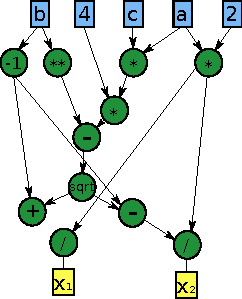
\includegraphics[width=0.4\linewidth]{Figures/Implementation/DFG.pdf}
  \caption{Data flow graph for the solutions (\ref{quadraticEquationSolution1},~\ref{quadraticEquationSolution2}) of a 
	   quadratic equation \eqref{quadraticEquation}. The nodes (green circles) are mathematical 
	   operations connected by edges (arrows) that show the data flow direction. Inputs and outputs
	   are marked as rectangular boxes. Reproduced from:
  \href{http://web.cecs.pdx.edu/mperkows/temp/JULY/data-flow-graph.pdf}{web.cecs.pdx.edu}}
  \label{fig:DFG}
\end{figure}

A simple example of a DFG is displayed in \autoref{fig:DFG}, which is a visualization of the flow of data
for the (real) solutions 
\begin{subequations}
\begin{align}
 x_1 &= \frac{-b + \sqrt{b^2 - 4ac}}{2a}  \label{quadraticEquationSolution1} \\
 x_2 &= \frac{-b - \sqrt{b^2 - 4ac}}{2a}
 \label{quadraticEquationSolution2}
\end{align}
\end{subequations}
of a quadratic equation
\begin{equation}
 ax^2 + bx + c = 0
 \label{quadraticEquation}
\end{equation}
We observe that each node (green circles)
contain the mathematical operations needed to compute
(\ref{quadraticEquationSolution1},~\ref{quadraticEquationSolution2}), while the arrows
(edges) show what data each node recieve and where
the output is sent. The inputs and outputs
of the graph is marked with rectangular
boxes. 

TensorFlow was originally developed by 
the Google Brain Team% 
\footnote{\href{https://research.google.com/teams/brain/}{research.google.com}}
with the purpose of conducting machine learning and 
deep neural networks research, but is 
applicable in other domains as well, e.g.\ for
solving partial differential equations. 
The package incorporates
a wide variety of machine learning algorithms, including
convolutional neural networks and recurrent neural networks.
A computation expressed using TensorFlow can 
be executed on a wide variety of devices and systems, 
from mobile phones to large-scale distributed systems
and GPUs. 

In this chapter we will go through a simple 
example on how to build a computational graph 
with TensorFlow, and how to train a
feed-forward neural network. We begin with a brief discussion on how to install the software. 

\section{Installing TensorFlow}
The easiest way to install TensorFlow on Ubuntu%
\footnote{\href{https://www.tensorflow.org/install/install\_linux}{www.tensorflow.org/install/}}
is to use pip%
\footnote{\href{https://pip.pypa.io/en/stable/}{pip.pypa.io/en/}},
a package management system for software written in 
Python, installed with the command
\begin{lstlisting}[language=bash]
 $ sudo apt-get install python-pip python-dev
\end{lstlisting}
TensorFlow can be installed with or without GPU 
support. The GPU version requires a system with
 CUDA-enabled NVIDIA GPUs
\footnote{\href{https://developer.nvidia.com/cuda-gpus}
{https://developer.nvidia.com/cuda-gpus}}. 
We have used the CPU version for the
development of our code, which is installed
with the command
\begin{lstlisting}[language=bash]
 $ pip install tensorflow
\end{lstlisting}
A simple
\begin{lstlisting}[language=bash]
 $ python -c "import tensorflow"
\end{lstlisting}
will test if the installation was succesful. 

\section{TensorFlow basic usage} \label{sec:TensorFlowBasic}
TensorFlow relies on highly-optimized
C\texttt{++} for its computations, but offers
APIs \footnote{\href{https://www.tensorflow.org/api_docs/}
{https://www.tensorflow.org/api\_docs/}}
in both Python,
C\texttt{++} and a few other languages. 
The \texttt{Python} API is at present the most
complete, the easiest to use and the best documented.
We have therefore chosen to use Python
to train neural networks. For a discussion
on ways to import a trained NN to C\texttt{++} see
\autoref{sec:extendingLammps} and \autoref{sec:transferNN}. 

\subsection{Hello world}
As already mentioned, a TensorFlow computation
is described by a graph which consists of nodes
that communicate with multi-dimensional arrays along
interconnected edges. Each node has zero or more
outputs, and represents the instantation
of an \textit{operation}. Each operation
occurs within a so-called \textit{session}. 
A \texttt{Hello world!} program can be written as
\begin{minted}{Python}
import tensorflow as tf

hello = tf.constant('Hello world!')
sess = tf.Session()
print sess.run(hello)
# --> Hello world!
\end{minted}
This simple example outlines the general
workflow for building a TensorFlow graph,
\begin{enumerate}
 \item Declare nodes (operations)
 \item Initiate a session
 \item Run operations within session
\end{enumerate}
The only operation in the above example
is the built-in TF constant that holds the 
\texttt{Hello world!} string, and the 
corresponding DFG only consists of one node. 
In more involved examples, visualizing 
the DFG can be useful for finding out how 
the script works. This is done with the 
included TF visualization tool TensorBoard.
We will now look at how to construct a neural network with TF and
visualize the corresponding DFG. 

\subsection{Creating a neural network} \label{sec:TensorFlowCreatingNN}
In \autoref{sec:MLPmodel} we demonstrated that a NN can be constructed 
as a set of matrix-vector multiplications and additions which are input to certain activation functions. 
The equations for evaluting a NN were \eqref{forwardPropMatrix},
\begin{subequations}
 \begin{align}
  \vec{u}_l &= \mathrm{W}_l\vec{y}_{l-1} + \vec{b}_l \label{preActivation2} \\
  \vec{y}_l &= f_l(\vec{u}_l) \label{activation2}
 \end{align}
\end{subequations}
We now want to construct a NN with 3 inputs neurons, one hidden layer with 10 neurons and 1 output neuron. 
We use the sigmoid \eqref{sigmoidActivationFunction} activation function for the hidden layer, while 
the output layer have the identity activation function \eqref{outputActivation}.
This can be achieved with the following Python script,
\begin{minted}{python}
import tensorflow as tf

# NN parameters
inputs  = 3
nodes   = 10
outputs = 1

# declare input tensor
inputLayer = tf.placeholder( tf.float32, [None,inputs] )

# weights input layer -> hidden layer and biases hidden layer
W1 = tf.Variable( tf.random_normal([inputs,nodes]) )
b1 = tf.Variable( tf.constant(0.1, shape=[nodes]) )

# activation hidden layer
preAct1 = tf.add( tf.matmul(inputLayer, W1), b1 ) 
act1 = tf.nn.sigmoid(preAct1)

# weights hidden layer -> output layer and bias output layer
W2 = tf.Variable( tf.random_normal([nodes,outputs]) )
b2 = tf.Variable( tf.constant(0.1, shape=[outputs]) )

# activation output layer
preActOutput = tf.add( tf.matmul(act1, W2), b2 ) 
activationOutput = preActOutput
\end{minted}
There are several aspects of the TensorFlow Python API to comment on here. 
We observe that the input layer is declared as a TF \texttt{placeholder}. This is a special
type of TF tensor that is not initialized with any values, but is rather fed with data on its execution.
Specifying the first component of its shape as \texttt{None} signifies that we can supply an arbitrary 
number of data points simultaneously.
These properties enables the same NN to be evaluated for different data vectors of varying size on-the-fly during training, 
explained in more detail below. 

The weights and biases are declared as TF \texttt{Variables}. These are the trainable parameters 
of the computational graph, and are normally constructed as random numbers. In the present case,
the weights are normally distributed numbers while the biases are all set to the same value 0.1. 
We note that the shapes of the weight matrices and bias vectors are in accordance with the description in 
\autoref{sec:MLPmodel}.

The activations (outputs) of each layer are calculated according to \eqref{preActivation2} and \eqref{activation2}. 
Together with the input \texttt{placeholder}, these are of type \texttt{tf.Tensor}, i.e.\ nodes in the computational 
graph. 

\subsection{Visualizing the graph}
We can use TensorBoard to visualize the DFG of the above script. The DFG for the present example is quite
simple, but for more involved models it quickly becomes difficult to keep track of all the different components. 
A convenient tool to order and group the DFG is \textit{name scoping}. Both \texttt{Tensors} and \texttt{Variables} can 
be name scoped and TensorBoard employs this information to define a hierarchy of the nodes in the graph. 
An example of name scoping is
\begin{minted}{Python}
 with tf.name_scope('layer1'):
    W1 = tf.Variable( tf.random_normal([inputs,nodes]), name='weights')
    b1 = tf.Variable( tf.constant(0.1, shape=[nodes]), name='biases')
\end{minted}
which results in the following names,
\begin{itemize}
 \item \texttt{layer1/weights}
 \item \texttt{layer1/biases}
\end{itemize}
Additionally, TensorBoard will group the two variables together under \texttt{layer1}. 
To save the graph to file we have to start a TF session. The following script 
deploys name scoping, initiates a session and writes the DFG to file,
\begin{minted}{python}
import tensorflow as tf

# NN parameters
inputs = 3
nodes = 10
outputs = 1

with tf.name_scope('inputLayer'):
    inputData = tf.placeholder(tf.float32, [None,inputs], name='inputData')

with tf.name_scope('layer1'):
    
    W1 = tf.Variable( tf.random_normal([inputs,nodes]), name='weights' )
    b1 = tf.Variable( tf.constant(0.1, shape=[nodes]), name='biases' )
 
    preAct1 = tf.add( tf.matmul(inputData, W1), b1, name='preActivation' ) 
    act1 = tf.nn.sigmoid(preAct1, name='activation')

with tf.name_scope('outputLayer'):
    
    W2 = tf.Variable( tf.random_normal([nodes,outputs]), name='weights' )
    b2 = tf.Variable( tf.constant(0.1, shape=[outputs]), name='biases' )

    preActOutput = tf.add( tf.matmul(act1, W2), b2, name='preActivation' ) 
    actOutput = tf.identity(preActOutput, name='activation')
    
# initialization node
initOperation = tf.global_variables_initializer()

# start session
with tf.Session() as sess:
    
    # initialize all variables
    sess.run(initOperation)
    
    # write summaries
    tf.summary.FileWriter('Summaries', sess.graph)
 
\end{minted}
There are two new TF function calls to comment on in this script. First, we have the line
\begin{minted}{Python}
 initOperation = tf.global_variables_initializer()
\end{minted}
Constants are initalized when we call \texttt{tf.constant}, and their value can never change. 
By contrast, variables need to be initialized using a seperate operation within a session. 
The function \texttt{tf.global\_variables\_initializer} adds such an operation to the graph, which initializes
all global variables when run with \texttt{sess.run(initOperation)}. 

Secondly, the graph is written to file for visualization with the function \texttt{tf.summary.FileWriter}. 
The first argument is the location of the files, while the second is the graph that is launched in the
present session. 

The resulting graph is displayed in \autoref{fig:graphExample}. 
By default, only the top of the hierarchy defined by name scoping is shown. In our case, this
is the three NN layers. In this figure, the output layer is expanded to reveal all the nodes in this scope. 
The nodes are marked by ellipses, while the rectangles are namespaces defining another level in the hierarchy, 
each containing more nodes. The edges show how the nodes are connected% 
\footnote{Each TF variable and constant are actually made up of several nodes, including \textit{assign} and 
\textit{read} operations. See TF API for more information.}.
\begin{figure}[H]
\centering
  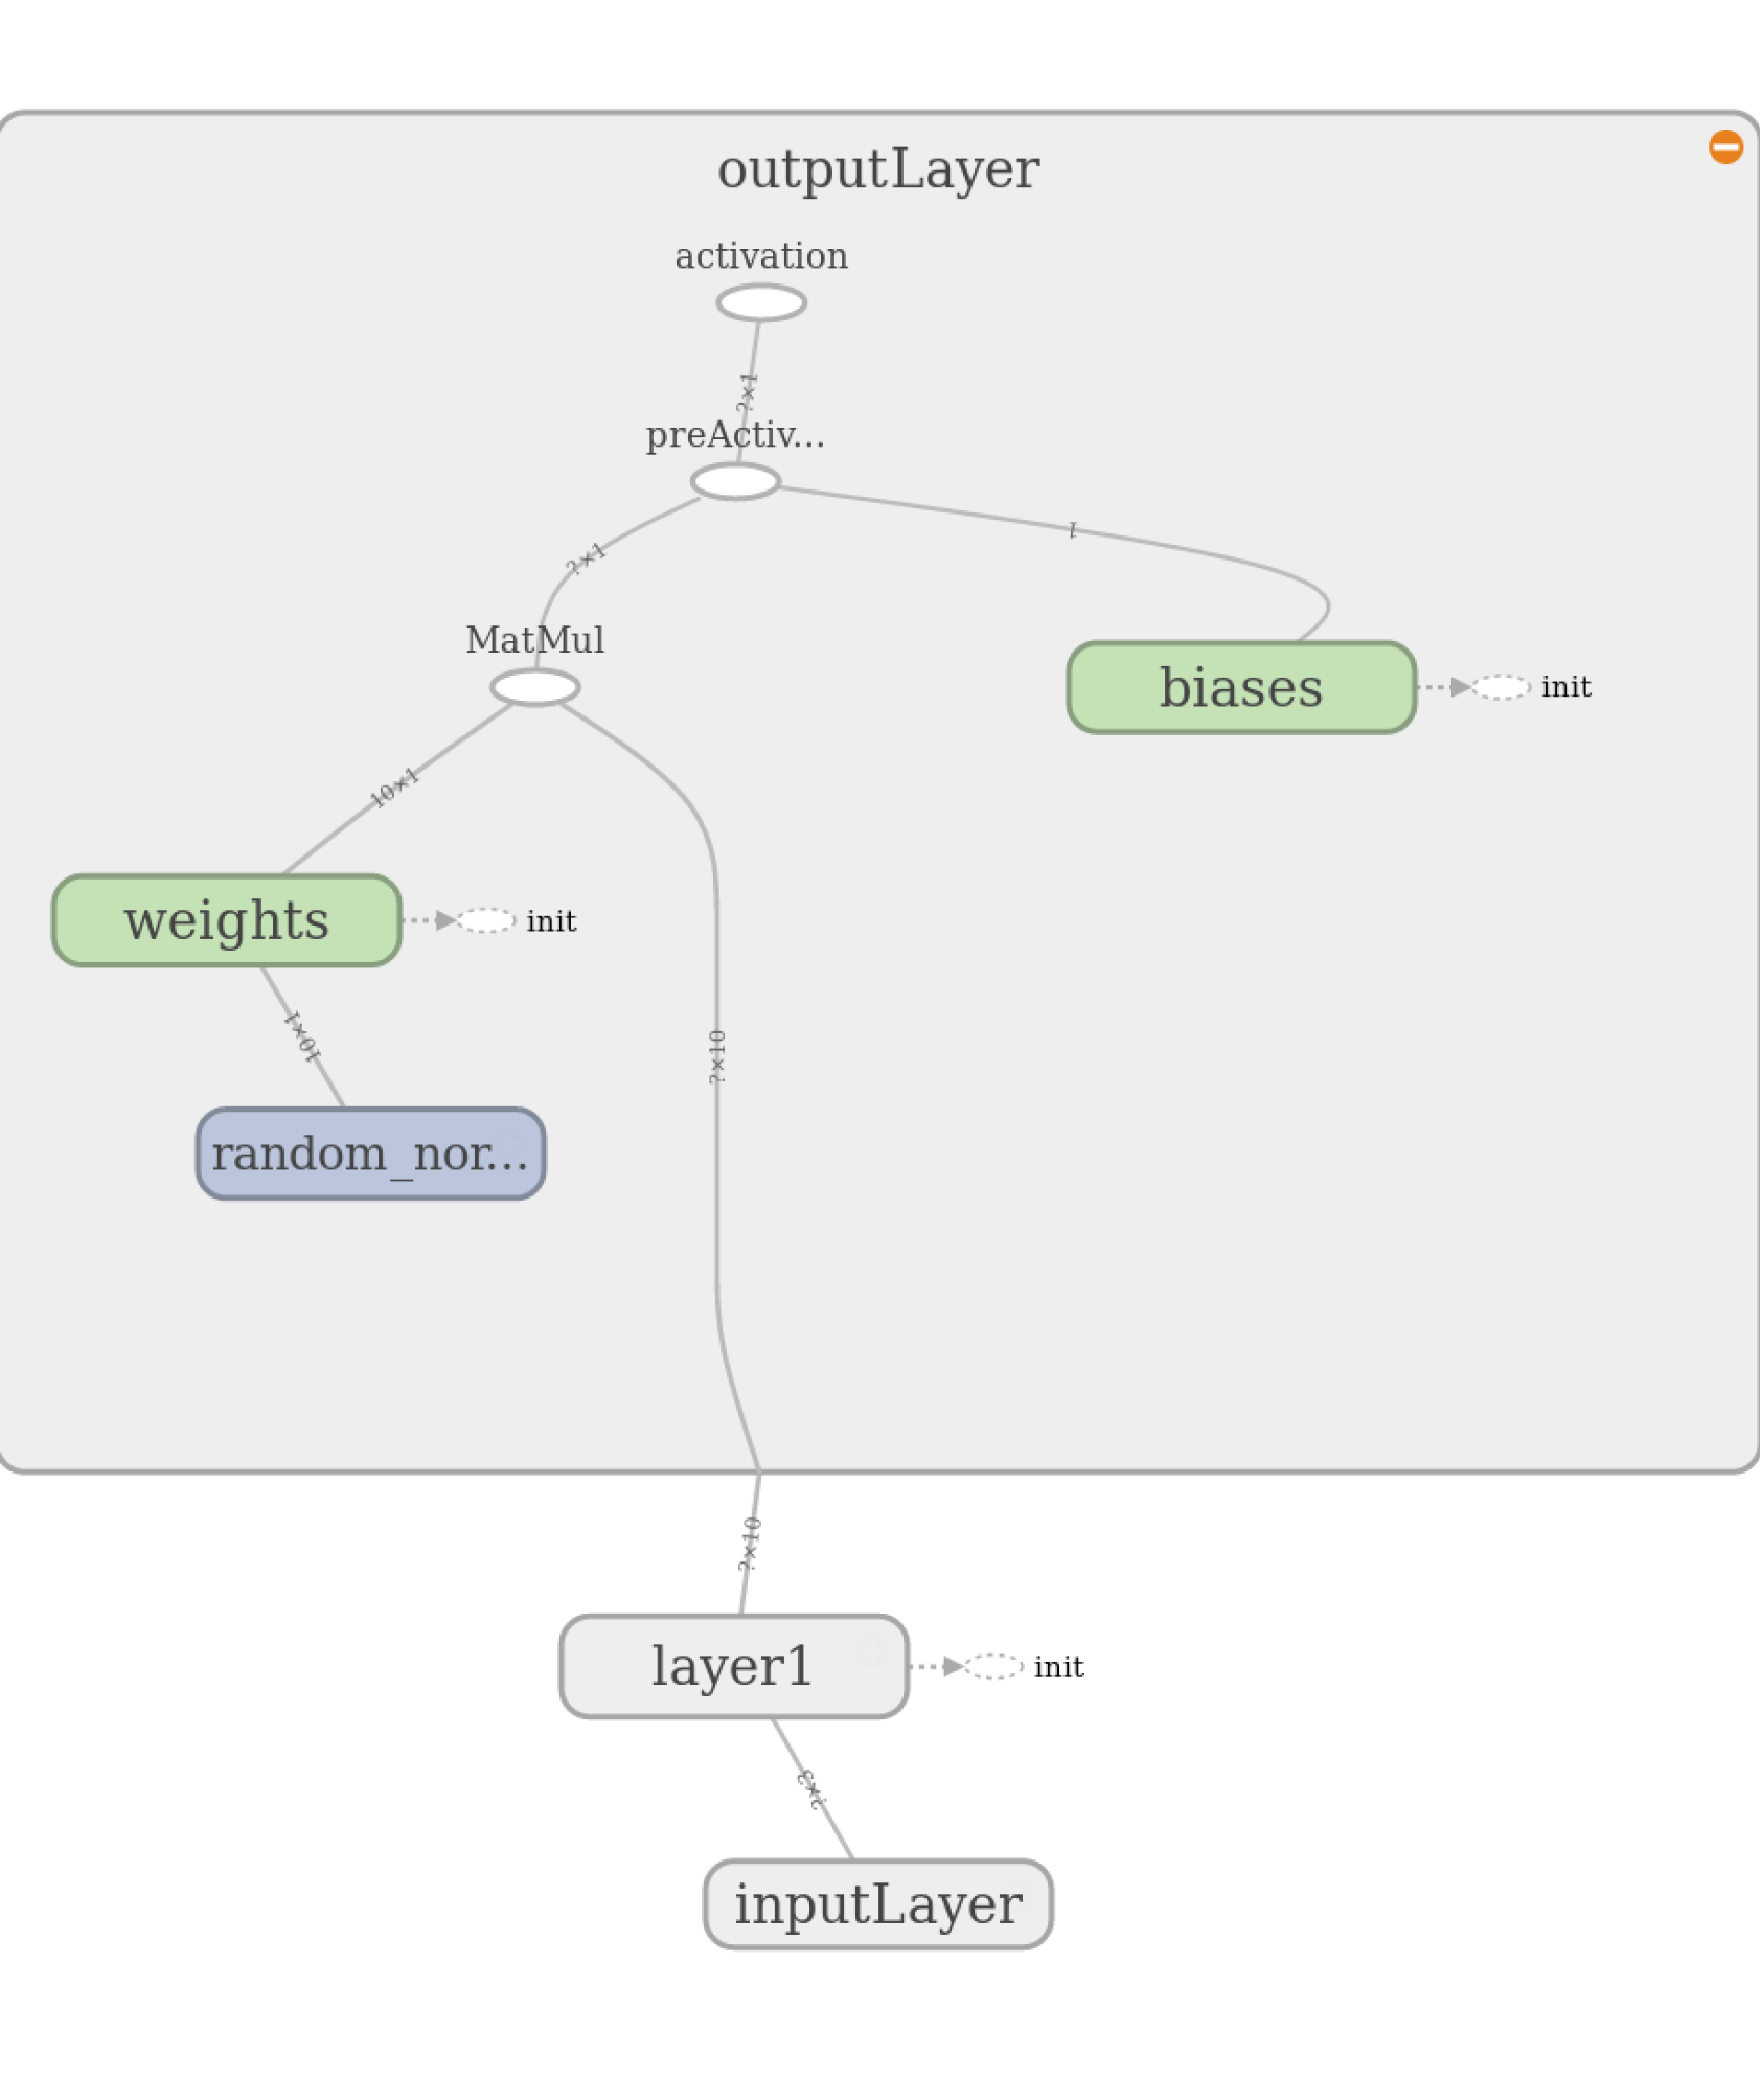
\includegraphics[width=0.7\linewidth]{Figures/Implementation/tensorBoardExample.pdf}
  \caption{Example of a computational graph in TensorBoard of a NN consisting of an input layer, one 
	   hidden layer and an output layer. Nodes are marked by ellipses, the rectangles are namespaces
	   containing several nodes.} 
  \label{fig:graphExample}
\end{figure}
\noindent Next, we will demonstrate how to train a NN with TensorFlow. 

\subsection{Training a NN with TensorFlow} 
To train the NN described in the previous section, we need two additional components:
a cost function and an optimizer. The mean-square-error cost function \eqref{quadraticCost} is available as a 
built-in function in TF, \texttt{tf.nn.l2\_loss}. To compute the error, we need to supply known 
target values that is fed into a new \texttt{placeholder},
\begin{minted}{python}
 outputData = tf.placeholder(tf.float32, [None,outputs], name='outputData')
\end{minted}
The cost function is now defined as
\begin{minted}{python}
 cost = tf.nn.l2_loss( tf.subtract(actOutput, outputData), name='cost')
\end{minted}
This adds an operation to the graph that calculates the mean-square-error between the NN prediction \texttt{actOutput}
on the data set
and the known target values \texttt{outputData}. In this work, the input data is configurations of atoms, 
while the target values are the potential energies of these configurations. 

A number of gradient descent optimizers are implemented in TensorFlow, including
vanilla gradient descent \eqref{gradientDescent}, Momentum \cite{Qian99}, Adagrad \cite{Duchi11}, 
Adadelta \cite{Zeiler12} and Adam \cite{Kingma14}.
To add the Adam optimizer operation to the graph, we simply write
\begin{minted}{python}
optimizer = tf.train.AdamOptimizer()
trainStep = optimizer.minimize(trainCost)
\end{minted}
To sum up, we have added the following to the script in the previous section (now with name scoping),
\begin{minted}{python}
outputData = tf.placeholder(tf.float32, [None,outputs], name='outputData')

# cost function
with tf.name_scope('cost'):
    error = tf.subtract(actOutput, outputData, name='deviation')
    cost = tf.nn.l2_loss(error, name='L2norm')

# optimizer
with tf.name_scope('optimizer'):
    optimizer = tf.train.AdamOptimizer(learning_rate=0.001, name='Adam')
    trainStep = optimizer.minimize(trainCost, name='trainStep')
\end{minted}
\begin{figure}[b]
\centering
  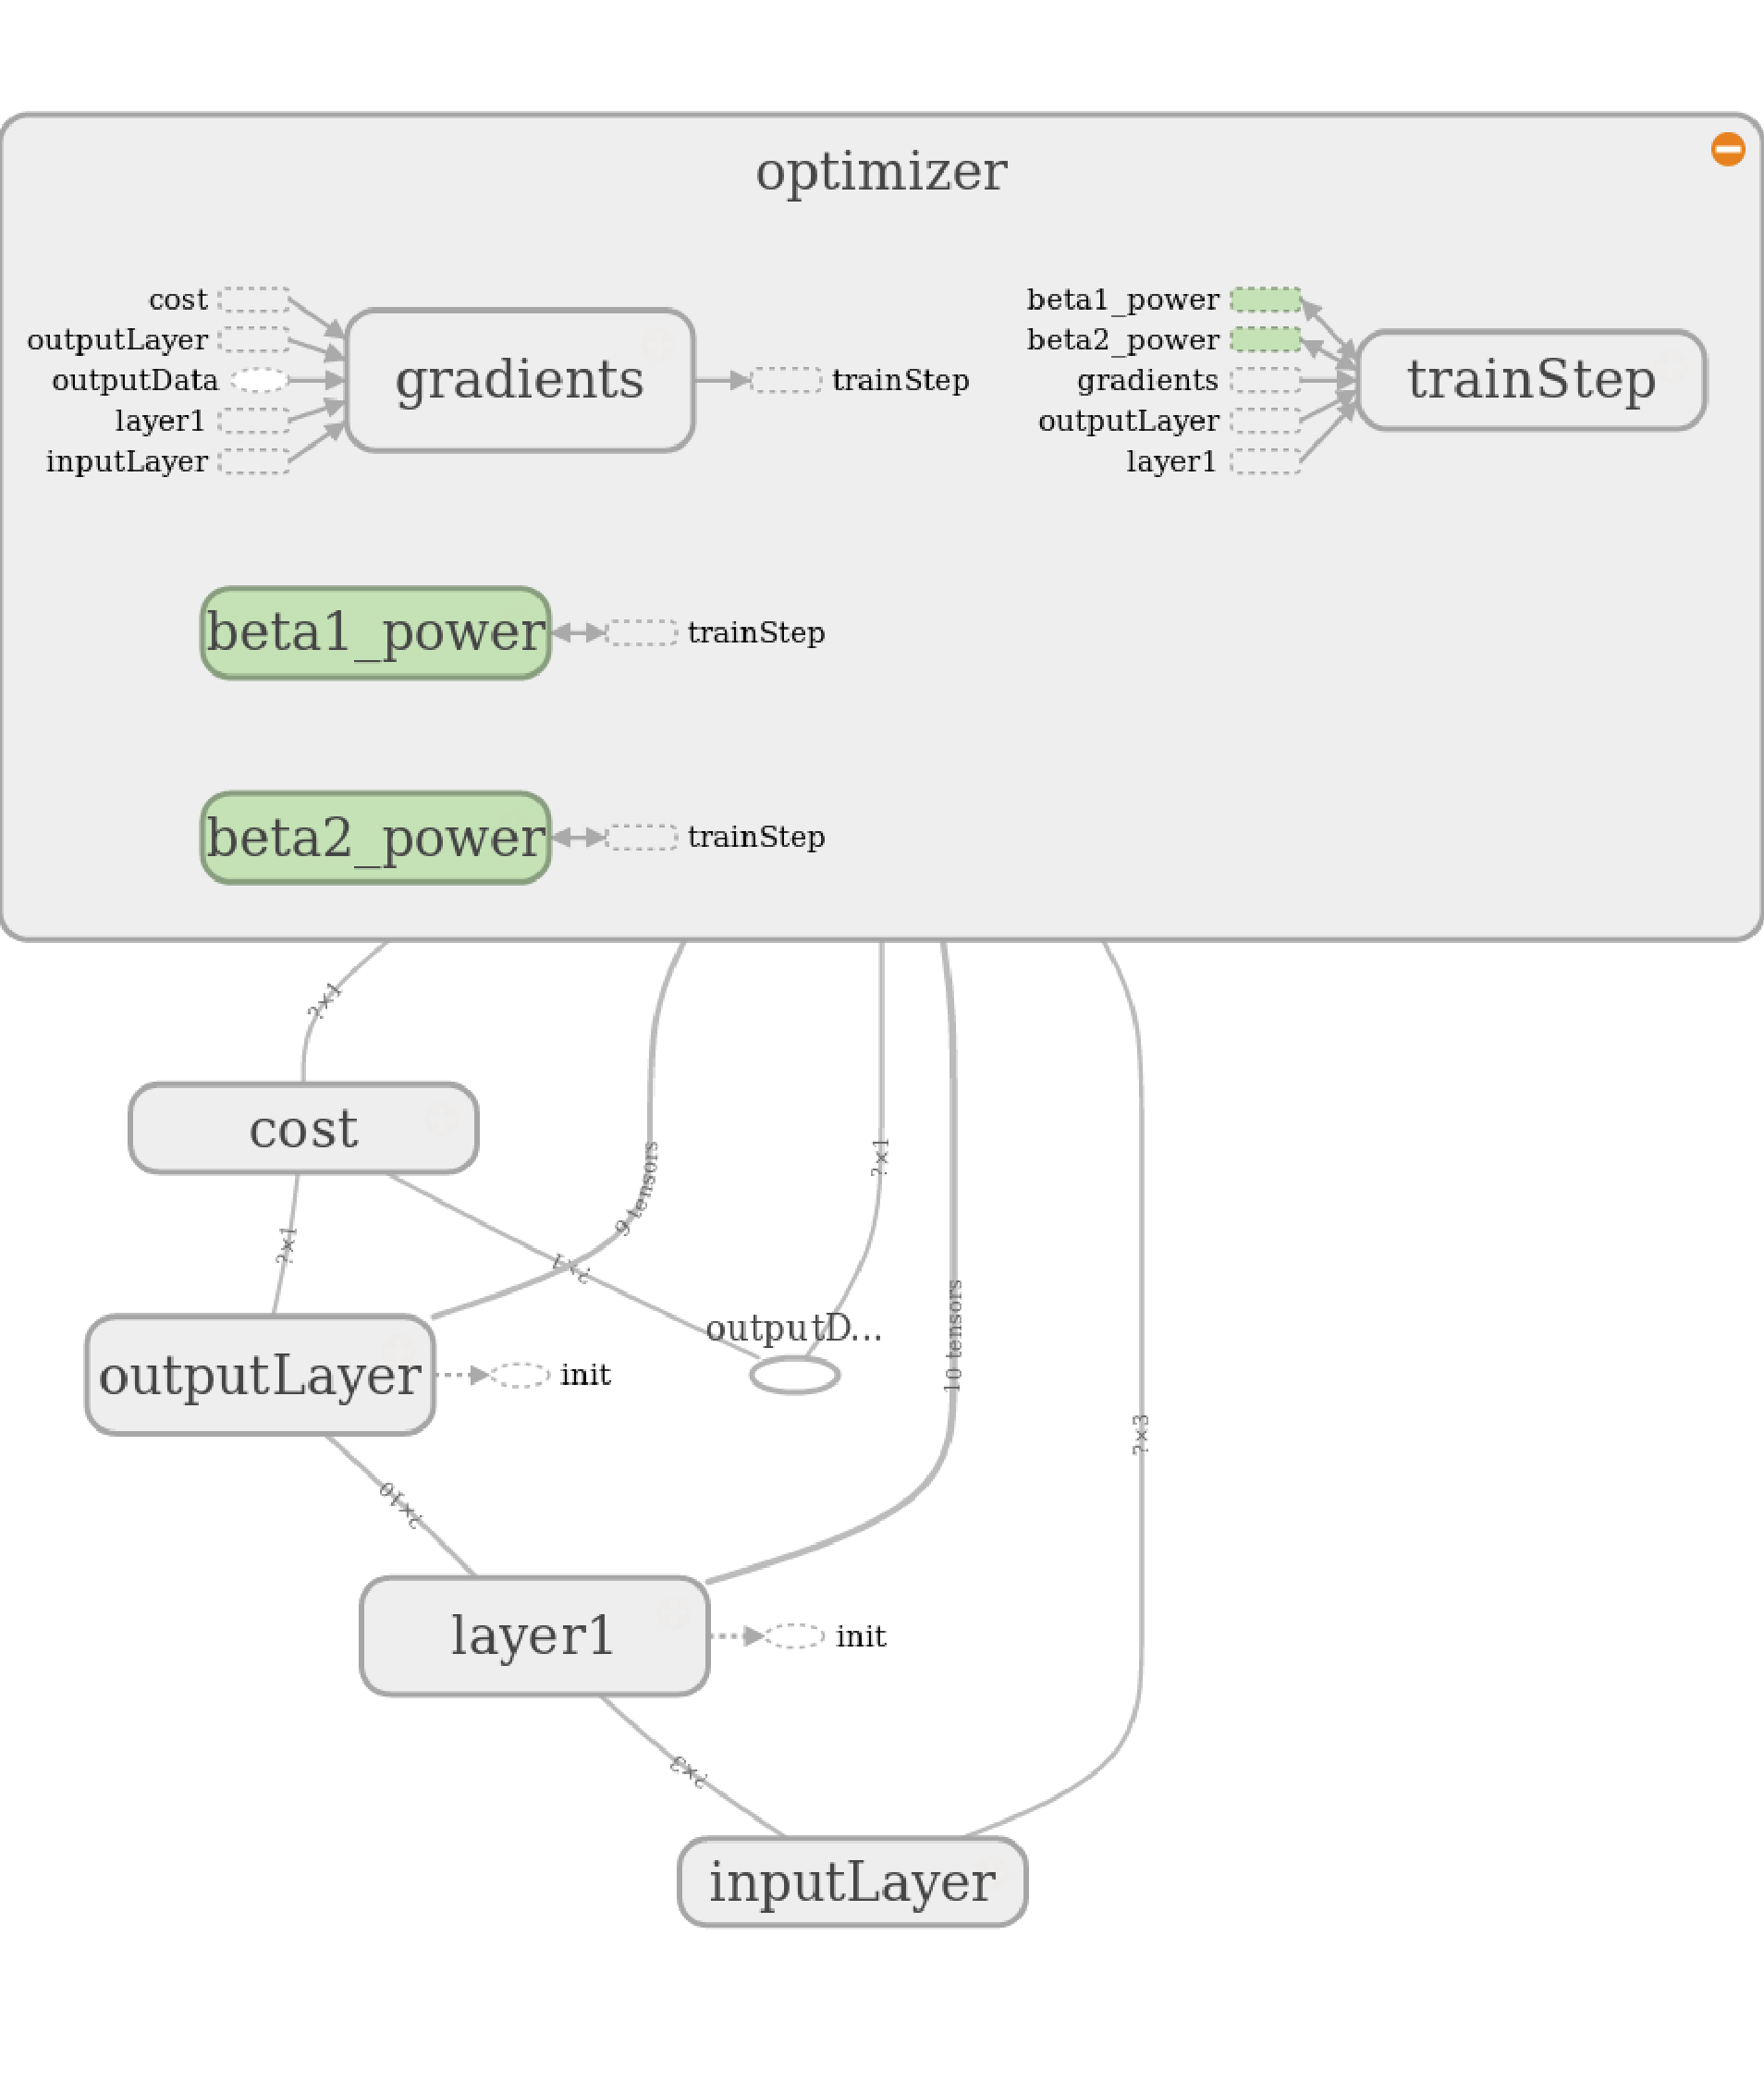
\includegraphics[width=0.8\linewidth]{Figures/Implementation/tensorBoardTraining.pdf}
  \caption{Example of a computational graph in TensorBoard for training a NN consisting of an input layer, one 
	   hidden layer and an output layer. Nodes are marked by ellipses, the rectangles are namespaces
	   containing several nodes. A cost function describing the error of the NN fit and an optimizer that minimizes
	   this error is included in the graph. The optimizer namespace is expanded to display its contents:
	   \texttt{gradients} computes the gradient of all nodes in the graph, \texttt{trainStep} implements
	   the algorithm for updating the NN parameters, while \texttt{beta1\_power} and \texttt{beta2\_power}
	   are the parameters of the Adam optimizer algorithm.}
  \label{fig:tensorBoardTraining}
\end{figure}
The resultant graph can be seen in \autoref{fig:tensorBoardTraining}. 
The optimizer namespace is expanded to display its contents. 
We observe that the optimizer is connected directly to all other parts of the graph, enabling it
to compute the derivative of the cost function with respect to all the weights and biases. This task is
performed by the \texttt{gradients} operation, that in turn sends the total gradient to \texttt{trainStep}, 
which implements the Adam algorithm for updating the NN parameters. 

We are now ready to launch this graph in a training session. We assume that input data
and target values are available as \texttt{NumPy} arrays \texttt{xTrain} and \texttt{yTrain} respectively. 
The code example implements the different variants of gradient descent described in \autoref{sec:gradientDescentVariants}. 
\begin{minted}{python}.
for epoch in xrange(numberOfEpochs+1): 
    
    # for shuffling the data set
    indicies = np.random.choice(trainSize, trainSize, replace=False)
    
    # offline learning / batch gradient descent
    if batchSize == trainSize:    
	
	# pick whole set in random order               
	xBatch = xTrain[indicies]
	yBatch = yTrain[indicies]
	
	# train
	sess.run(trainStep, 
		 feed_dict={inputLayer: xBatch, outputData: yBatch})
	
    # online learning
    else:                      
	# loop through whole set, train each iteration
	for b in xrange(numberOfBatches):
	    batch = indicies[b*batchSize:(b+1)*batchSize]
	    xBatch = xTrain[batch]
	    yBatch = yTrain[batch]
	    
	    # train
	    sess.run(trainStep, 
	             feed_dict={inputLayer: xBatch, outputData: yBatch})
	    
    trainError = sess.run(cost, 
                        feed_dict={inputLayer: xBatch, outputData: yBatch})
\end{minted}
We observe that the training step is performed with the single line,
\begin{minted}{python}
sess.run(trainStep, feed_dict={inputLayer: xBatch, outputData: yBatch})
\end{minted}
which runs the \texttt{trainStep} operation defined above. This operation initiates a series of
calculations that is performed automatically by TensorFlow. 
First, the NN is evaluated on the training batch \texttt{xBatch} and the output is compared to the corresponding
batch of target values \texttt{yBatch}. The training batch is fed to the NN through the placeholder
\texttt{inputLayer}, while \texttt{outputData} receives the target batch. Next, the cost function 
is calculated, and the error is backpropagated through the DFG to obtain its gradient. Finally, 
the Adam update rule is applied and the weights and biases adjusted. 



\chapter{Constructing a neural network potential} \label{sec:constructingNNP}
The general workflow for constructing and applying a high-dimensional neural network potential (NNP) is as follows: 
\begin{enumerate}
 \item Generate training data relevant for the intended application of the NNP.
 \item Train a NN to fit the data, employing a suitable set of hyperparameters.
 \item Use the analytical expression for the eventual NNP as a potential in MD simulations.
\end{enumerate}
In this chapter we will go into details regarding these three steps. 
We describe different ways of assembling 
an adequate reference set for the NN, which is the most crucial factor for the performance of 
the final potential. Further, we discuss how suitable hyperparameters can be determined, including the 
symmetry function parameters. Lastly, we compare the performance of two different methods for evaluating a
trained NN in simulations. 




\section{Selecting the reference set} \label{sec:selectingTrainingData}
The number of possible configurations of atomic or molecular systems quickly grows very large. 
Consider for instance water $\textrm{H}_2\textrm{O}$, which is a three-body molecule. The configuration of the
three atoms can be described by three internal coordinates, each with a certain range of values. 
If each range is divided into $N$ equal segments, the total number of distint configurations is $N^3$. 
If we were to construct an \textit{ab inito} potential that characterizes this system, we would have to compute the energies 
and forces of all these configurations. 
Such a brute-force approach may be feasible for a three-atom molecule, but for more complicated systems
it quickly becomes practically impossible due to the computational cost. 

In this work we do not use \textit{ab inito} methods to compute energies and forces, but this problem is still highly relevant
due to the high-dimensional nature of our approach. The average number of neighbours for the Stillinger-Weber Si simulations
in this thesis is about $n=6$ (\autoref{sec:SiPotentialResults}), which is a small number compared to most other systems.  
This number is of great importance to the efficiency of the fitting process because it defines the dimensionality 
of the problem,
\begin{enumerate}
 \item When increasing $n$, each symmetry function is composed of 
 more terms. The number of terms $N_{terms}$ scales like $N_{terms} \propto n$ for the radial symmetry functions, 
 but for the angular symmetry functions we have that $N_{terms} \propto n^2$. 
 \item A larger $n$ leads in general to a larger configuration space to fit, thus additional symmetry functions and 
 a larger data set is required. 
 \item The number of NN parameters must also be increased to obtain the same error as for a lower-dimensional problem
\end{enumerate}
These observations demonstrate that performance is a critical factor whether we fit \textit{ab inito} data or 
not. However, we know that only a small subset of the possible configurations of a system is physically realizable. 
Most of the configurations will not be visited by a system obeying Newton's laws, and are therefore not important to
the dynamics. We thus need some kind of importance sampling method that adequately samples this subset. 
We realize that the obvious way to achieve this is to sample configurations from molecular dynamics simulations, which
yields precisely the subset we are looking for. 

\subsection{Iterative molecular dynamics sampling} \label{sec:iterativeMDsampling}
In this thesis we employ an iterative scheme to construct a NNP with data sampled from MD simulations. 
The method have been used by e.g. Raff et al \cite{Raff12} and Behler \cite{Behler11general}, and is as follows
\begin{enumerate}
 \item Sample an initial data set from MD simulations. \label{sample} 
 \item Calculate the energies and optionally the forces of this initial data set with a chosen method. \label{refEnergies}
 \item Train a NN on the data from \ref{sample}. with reference values from \ref{refEnergies}. to
 construct a preliminary NN potential.
 \item Carry out simulations using the NNP to find new relevant structures. 
 \item Compute the energies (and forces) of the new structures with the method from 2. and add them to the data set
 \item Train a NN on the extended data set to improve the NNP
 \item Repeat 4-6. until no new relevant configurations are found. 
  \label{NNPalgorithm}
\end{enumerate}
The idea is to improve the NNP iteratively and in a self-consistent 
way by applying it in MD simulations to find 
''holes'' in the data set, i.e.\ configurations on which the NNP predicts incorrect energies and forces. The process
is different depending on whether we are constructing a NNP from \textit{ab inito} electronic structure data
or reproducing known, empirical MD potentials. 

For the latter, we construct the initial data set by sampling configurations from MD simulations that is relevant
for the intended applications of the NNP. Furthermore, we are extracting both coordinates and energies from the simulations, i.e.\
we get both the input data in step 1 and the target values in step 2 simultaneously. To compute the energies in
step 4, we simply run a pseudo-simulation on the new structures. This is easily done in LAMMPS by using 
the \texttt{rerun} command, which tells LAMMPS to compute the energies and forces of atomic configurations 
supplied from file without doing any integration. 

When constructing an \textit{ab inito} NNP however, we are immediately faced with a problem when trying to execute this process: 
to run MD simulations in step 1 we need the PES we are trying to develop. 
This is often termed as the ''self-starting problem'', 
and several procedures have been suggested for handling it. 

One option is obviously to generate random configurations. This does however take us back to the 
original problem discussed in the beginning of this chapter: The large configuration space volume of
high-dimensional systems enforces the use of importance sampling methods. 
It is highly unlikely that random sampling will yield the important regions of configuration space, thus 
vast amounts of data is needed. Nonetheless, random sampling can be applicable to small systems of 1-3 atoms where
the complete configuration space can be represented without too much effort, see \autoref{sec:LJValidation}. 

Another option is to use chemical intuition to select certain configurations of 
the system under investigation. 
For instance, if a specific chemical reaction is studied, one can use previous knowledge about this reaction to 
select configurations along the reaction path \cite{Ischtwan94}. The disadvantage of this approach is that
such information is not always available. 

A more effective method has been presented by Raff et al.\ \cite{Raff05}, where a semi-empirical
potential has been deployed to initiate the sampling. If a reasonable potential is chosen and an adequate
sampling method is devised (discussed below), several thousand physically relevant structures can be obtained
that will constitue the initial data set. It has also been shown \cite{Raff05} that the final PES obtained 
by the iterative sampling of MD trajectories is not sensitive to the choice of the empirical surface employed 
in the initial step. 

In this thesis we do not construct \textit{ab inito} NNPs, thus we will not go into further details
of the above methods. 

\subsection{Sampling algorithms} \label{sec:samplingAlgorithms}
We have seen that MD simulations supply the data that is needed to construct a NN potential, but we 
also have to consider how this sampling should be performed to identify new relevant structures.
NNs have a very flexible functional form which makes them able to accurately fit data sets, 
but they can also yield potentially large energy and force errors 
when evaluated for configurations that are very different from the ones included in the data set.
It is therefore of vital importance to include all structures that are relevant for the intended
application of the NNP.

Sampling methods should in general be optimized to produce a reasonably uniform density of 
data points in those regions of configuration space that are relevant to the application of the fit \cite{Raff12}. 
If there are regions with very high point density compared to others, the NN will be trained to accurately fit these, 
at the cost of regions that are poorly represented. An exception to this rule is regions where the potential gradient, or forces, 
are large. These regions, typically configurations where two atoms are close to each other and experience strong
repulsive forces, are the most difficult for the NN to fit, 
and should therefore have a higher density. 

\subsubsection{Initial sampling}
The initial data set is supposed to function as a starting point for the construction of the NNP. 
In this work we use empirical MD potentials to do the initial sampling. Before the process is initiated, 
we must decide on the specific application for the NNP that we want to develop. This entails 
defining a range of temperatures, pressures etc.\ that the final NNP will be valid for, and sample
configurations based on these. 

The time interval between selecting configurations during the MD simulations must also be decided. 
One alternative is to simply sample points at constant time intervals. This approach will
however result in a non-uniform density of data points considering that atoms spend most of their time
in regions where the forces are small, at least in equilibrium MD. 

To sample configuration space with something close to a uniform density, the time interval $\tau$ between 
sampling needs to be a function of the atomic accelerations (or forces). One such variable 
interval sampling algorithm, suggested by Pukrittayakamee et al.\ \cite{Pukrittayakamee09}, is given as
\begin{equation}
 \tau = 
\begin{cases}
\textrm{floor}\left[\alpha/a_{\textrm{max}}\right]\Delta t, 
&\textrm{if floor}\left[\alpha/a_{\textrm{max}}\right] > 0 \\
\textrm{floor}\left[\alpha/a_{\textrm{max}}\right]\Delta t + \Delta t, 
&\textrm{if floor}\left[\alpha/a_{\textrm{max}}\right] = 0
\end{cases}
\label{variableIntervalSampling}
\end{equation}
where $a_i$ is the absolute value of the acceleration of atom $i$, $\Delta t$ is the integration step size, 
$a_\textrm{max}$ is the maximum acceleration of a chosen molecule, and $\textrm{floor}(x)$ yields
the integer part of $x$. The constant $\alpha$ is system dependent and must be determined empirically. It is the value 
of $\alpha$ that determines the sampling frequency. We see from the second condition in \eqref{variableIntervalSampling} that
configurations with an acceleration $a_i > \alpha$ yields $\tau = \Delta t$, i.e.\ the shortest possible sampling
interval. On the other hand, if $a_i < \alpha$, the interval increases by a factor $\textrm{floor}(\alpha/a_\textrm{max})$. 
This approach ensures that we sample all configurations where the gradient of the PES is large, while skipping many
of the low-gradient regions of configuration space. 

We have chosen to use the forces $|\vec{F}_i| \propto a_i$ instead of the accelerations, simply because they are
readily available in LAMMPS. When sampling systems with periodic boundary conditions, we have to consider 
the way forces are updated during a simulation. In LAMMPS, any forces attributed to ghost atoms are added back 
to the originals after \textit{all} forces are computed. This is done in
\texttt{verlet.cpp},
 \begin{minted}{C++}
  if (pair_compute_flag) force->pair->compute(eflag,vflag);
  // ...
  if (force->newton) comm->reverse_comm();
 \end{minted}
The first line computes the forces on all atoms with the chosen \texttt{pair\_style} potential, while
the second line communicates the forces on ghost atoms back to the original atoms according to Newton's third law. 
This means that to employ the algorithm
\eqref{variableIntervalSampling}, we need to sample configurations \textit{after} this reverse communication is
executed, if not the forces will be incorrect. This can be achieved by extending LAMMPS with a new \texttt{compute}%
\footnote{See \autoref{sec:lammpsInputScript} for an explanation of various LAMMPS input script commands, 
and \autoref{sec:extendingLammps} for a general description on how to add functionality to LAMMPS.},
as all \texttt{computes} and \texttt{fixes} are invoked after the
force calculations. 

We have made an additional modification to the algorithm \eqref{variableIntervalSampling}.  
Pukrittayakamee et al.\ \cite{Pukrittayakamee09} sample clusters of atoms for subsequent DFT calculations
of the energies of these clusters, and computes $\tau$ based on the maximum acceleration of an atom in a cluster. 
Our strategy is to select a few atoms, usually 1-10, and compute $\tau$ seperately for each of these atoms. When 
the sampling criterium is met, the coordinates of all neighbours relative to the central atom is written to file, 
as well as the potential energy the central atom experiences in the presence of its neighbours. These coordinates
and energies make up the input data and target values, respectively, for a NN to interpolate. 
Our modified sampling algorithm is thus as follows (written in a less convoluted way than above),
\begin{equation}
 \tau = 
\begin{cases}
  \textrm{floor}\left[\alpha/F_i\right], &F_i \leq \alpha \\
  1, &F_i > \alpha \\
  \tau_\textrm{max}, &\textrm{floor}\left[\alpha/F_i\right] > \tau_\textrm{max}
\end{cases}
\label{samplingAlgorithmModified}
\end{equation}
where $\tau$ is measured in units of $\Delta t$ and $\tau_\textrm{max}$ is the maximum value of $\tau$.
$F_i$ is the total force on atom $i$ including ghost contributions. 
We have implemented this sampling algorithm as follows,
\begin{minted}{c++}
// ...
// loop through atoms that is to be sampled
for (auto ii : chosenAtoms) {
    i = ilist[ii];
    itype = type[i]-1;

    double F = sqrt(f[i][0]*f[i][0] + f[i][1]*f[i][1] + f[i][2]*f[i][2]);

    // update tau every maxDelay step
    if ( !(myStep % maxDelay) ) {

      // no delay if force is larger than alpha
      if (F > alpha[itype]) tau[atomCount] = 1;

      // calculate delay if force less than alpha
      else {
        int factor = floor( alpha[itype] / F );
        if (factor > maxDelay) tau[atomCount] = maxDelay;
        else                   tau[atomCount] = factor;
      }
    }

    // decide whether to sample or not based on current value of tau for atom i
    if ( (myStep % tau[atomCount] > 0) && useAlgo) continue;

    double xi = x[i][0];
    double yi = x[i][1];
    double zi = x[i][2];
    
    // loop through neighbours of atom i 
    // write relative coordinates and atomic energy to file
    jlist = firstneigh[i];
    jnum = numneigh[i];
    for (jj = 0; jj < jnum; jj++) {
      j = jlist[jj];
      // ...
\end{minted}
The vector \texttt{chosenAtoms} contains the indicies of the atoms that are to be sampled. These indicies are decided
when the parameters of the employed potential is initiliazed with the input script command \texttt{pair\_coeff}. 
The variable \texttt{maxDelay} decides how often $\tau$ is updated, and serves as a maximum value of $\tau$. 
Its value does not change in the course of the simulation. 
\begin{figure}
\begin{minipage}{0.48\linewidth}
  \subcaption{}
  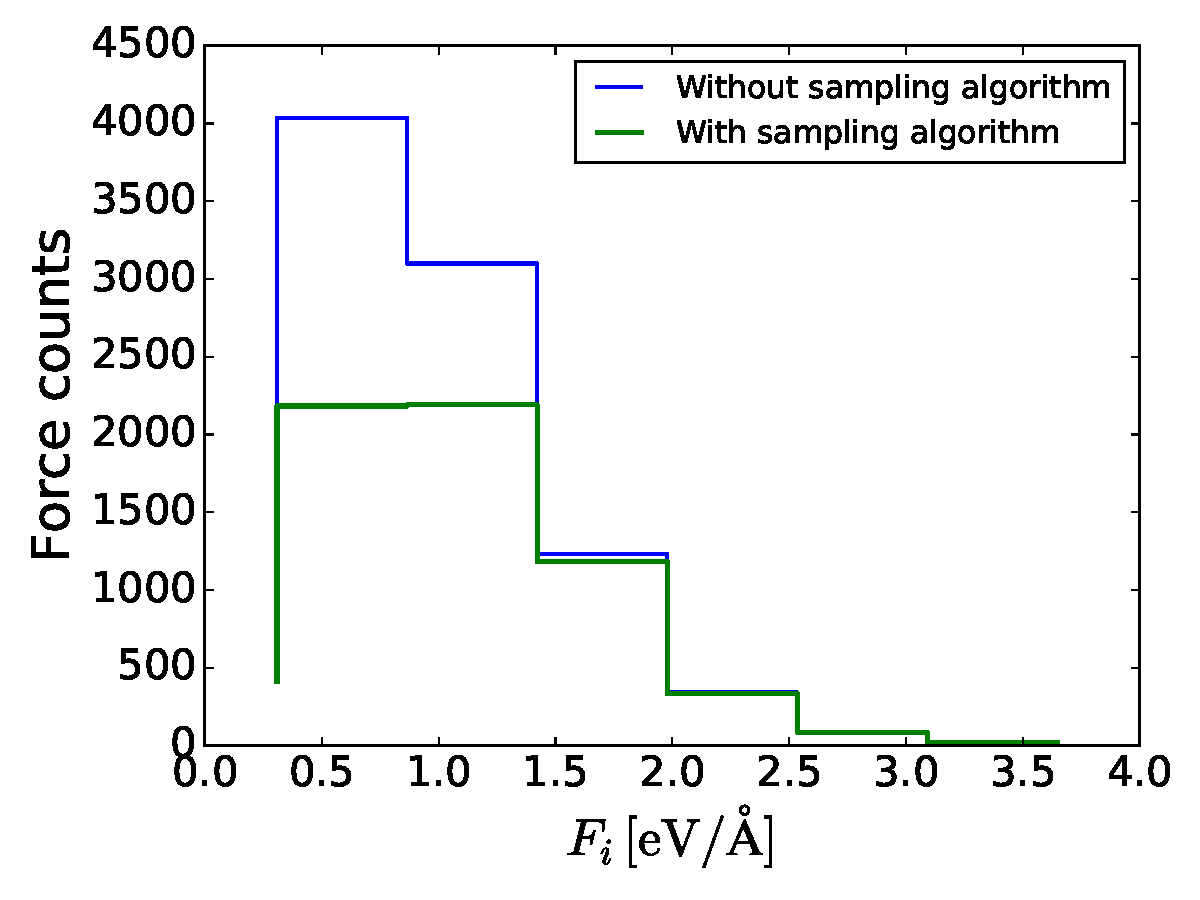
\includegraphics[width=\textwidth]{Figures/Implementation/forceDistSamplingAlgo.pdf}
  \label{fig:forceDistSamplingAlgo:a}
\end{minipage}
\quad
\begin{minipage}{0.48\linewidth}
\subcaption{}
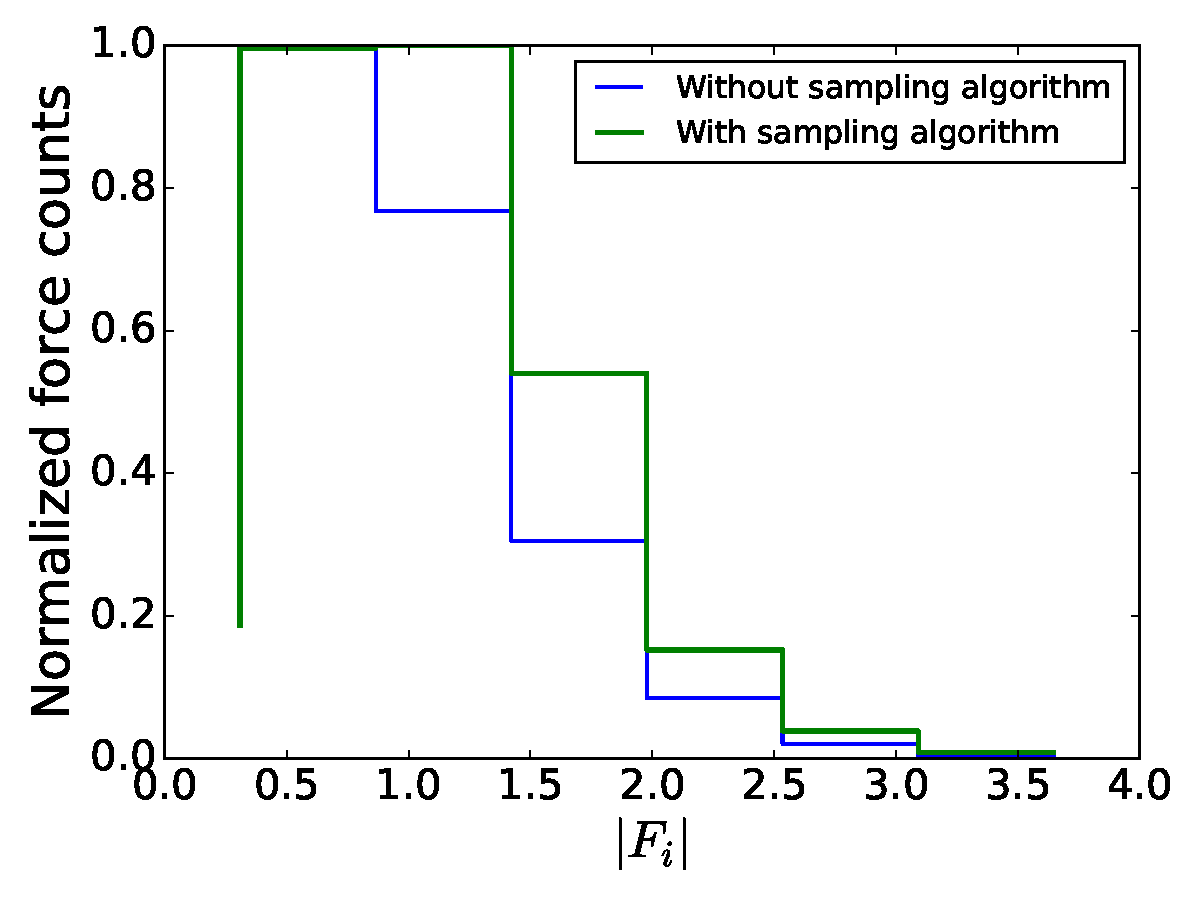
\includegraphics[width=\textwidth]{Figures/Implementation/forceDistSamplingAlgoNormed.pdf}
 \label{fig:forceDistSapmlingAlgo:b}
\end{minipage}
\vspace{-1ex}
  \caption{Distribution of forces for one Si atom in a quartz $\textrm{SiO}_2$ crystal with 
	   and withouth the use of the sampling algorithm \eqref{samplingAlgorithmModified}. 
	   The crystal consists of 576 atoms, with an initial temperature $T= \SI{1000}{\kelvin}$, 
	   run for $N = 10000$ time steps. The atoms are sampled from the microcanonical ensemble with
	   periodic boundary conditions.
	   Sampling algorithm parameters: $\alpha=3.0$ and 
	   $\tau_\textrm{max} = 10$.}
\label{fig:forceDistSamplingAlgo}
\end{figure}
\autoref{fig:forceDistSamplingAlgo} displays the distribution of forces for one Si atom in a MD simulation
of quartz $\textrm{SiO}_2$, with and withouth the use of the sampling algorithm \eqref{samplingAlgorithmModified}. 
We see from \autoref{fig:forceDistSamplingAlgo:a} that the 
sampling procedure cuts the number of low-gradient configurations significantly, 
while keeping all the environments corresponding to large forces. The resulting distribution is however not uniform, simply
because the ratio of force counts in the range $F_i = \SIrange{0}{2}{\angstrom}$ to the range $F_i = \SIrange{2}{4}{\angstrom}$
is too high originally.

One way to smooth the distribution further is to manually delete configurations after the simulation 
is finished, but then we risk removing relevant structures. The gradient of the PES is not the only way 
to measure the quality of the sampled set, the time aspect is also important. 
By selecting samples on-the-fly, we are guaranteed that the they are distributed somewhat uniformly in the time domain. 
Deleting structures blindly subsequent to the simulation is therefore not a good idea.

Another option is to sample different types of systems where the forces are more evenly distributed. 
Examples are non-periodic systems or systems containing only a few atoms. Also, it can be a good idea 
to do short simulations where the atoms start out in non-equilibrium positions to obtain configurations
that are not visited by systems with a regular lattice initial state. 

\subsubsection{Iterative sampling}
The initial data set is usually not sufficient to construct a stable neural network PES. 
It is difficult to identify all the relevant structures that the NN have to learn to perform well, and 
since there is always a small fitting error, the 
NNP will generate different trajectories than the PES that has been used to train it. The data set can be extended
by sampling new relevant structures from simulations using the preliminary NNP trained on the initial data set. 
In this way, new configurations
will ''naturally present themselves'', and the NNP will iteratively improve in a self-consistent way.

The obvious way to identify new structures not already in the initial data set is to evalate both the NNP and 
the PES we are trying to fit for each structure in an NNP MD simulation and compare the energies (and eventually 
the forces). If the energy deviation is above a certain treshold, the structure is added to the data set.
The simulations should be carried out under the conditions of the intended application of the NNP to ensure
that the relevant parts of configuration space are sampled.
After a certain amount of new data is added, 
the NN is trained on this extended data set and thus improved. Then, new simulations are carried out with the improved
NNP and so on, according to the iterative process described in the beginning of this chapter. 

This approach is easily feasible when the target PES is an empirical potential, but too computationally expensive 
in the case where electronic structure methods are employed. Raff et al.\ \cite{Raff05} have developed a sampling
algorithm called \textit{modified novelty sampling} that does not require any quantum mechanical calculations of
the energies of new structures. They describe the database as a set of vectors $\{\vec{q}\}$, where vector
$\vec{q}_i$ contains the internal coordinates of the $i_\textrm{th}$ cluster of atoms. New configurations
$\vec{q}_n$ are generated using the NNP trained on this data base and the 2-norm difference $\vec{d}$ between vectors
$\vec{q}_n$ and $\vec{q}_i$ are computed,
\begin{equation}
 \vec{d} = | \vec{q}_i - \vec{q}_n | = 
 \left[(\vec{q}_i - \vec{q}_n)\cdot(\vec{q}_i - \vec{q}_n)\right]^{1/2}
\end{equation}
for all clusters $i$. The difference vector is characterized by its minimum value $d_\textrm{min} = \textrm{min}(\vec{d})$ and 
the mean seperation distance $d_\textrm{mean} = \langle\vec{d}\rangle$. 
The basic idea is to add configuration point $\vec{q}_n$ to the database with high
probability if $d_\textrm{min}$ or $d_\textrm{mean}$ is large, but low probability if both 
$d_\textrm{min}$ and $d_\textrm{mean}$ are small. The energy output of the NNP are also included in the scheme, along with
a more involved selection algorithm. As this thesis only deals with empirical target potentials, the details will
not be further discussed here. 

In this work we use the Behler symmetry functions to transform atomic cartesian coordinates to vectors of symmetry values.
These functions act as descriptors of chemical environments, and should therefore be excellent candidates
to identify relevant structures during MD simulations without computing additional target energies. 
Behler has suggested two methods \cite{Behler11general} where these symmetry functions are employed to improve the NNP. 
The first and simplest method identifies structures that fall outside of the range of input values spanned by the data set. 
This is achieved by comparing the symmetry function vector of each atom during the MD simulation with 
the minimum and maximum values of each symmetry function in the database for the respective element. 
When such configurations are encountered, a warning can be issued and the structure sampled.  

The other scheme developed by Behler is called the \textit{multiple-NN method} and is used to identify 
structures that are within the range of existing symmetry values, but located
in parts of configuration space that are poorly represented in the reference set.
The idea is to use the high flexibility and reasonably fast training and evaluation of NNs to validate 
the potential. The procedure is as follows,
\begin{enumerate}
 \item Fit several NNs with different architectures to the same data set. All the NNs should be trained
 to the same accuracy. 
 \item Generate a large number of trajectories and corresponding energies using one of these NNPs in MD simulations.
 \item Recalculate the energies of the obtained trajectories using the other NNPs.
 \item Structures for which the energy disagreement between the different NNPs is significant should be added to 
 the data set.
\end{enumerate}
This method takes advantage of the poor extrapolation abilites of NNs: The energy predictions of the different NNPs will
be more or less random on structures that are far away from the training points. Thus, missing structures can 
be identified by comparing the energy predictions of the different NNPs on the genereated trajectories. The procedure 
also provides a criterion for determining the convergence of the PES without requiring the repeated computation 
of dynamic properties of the system under study. When, after several iterations of the multiple-NN method,
no problematic structures are found, the NNP should be reliable and ready for use. 

\subsection{Summary}
In this section we have presented several procedures to 
assemble the data set for the NN, which depends on how the target energies are computed. 
In this work, we know the PESs we are trying to fit, which are common empirical MD potentials. 
Therefore, the NNP can be validated simply by comparing its predictions to the target PES.  
On the other hand, if an \textit{ab inito} NNP is to be constructed, the underlying target PES is not known, 
and computing energies and forces of eventual new structures are expensive. Two methods circumventing
this problem has been described.

Still, there are several factors to consider when constructing the reference set, irrelevant of how the target PES looks like.  
We have implemented and employed a sampling algorithm \eqref{samplingAlgorithmModified} in this thesis to obtain a more uniform
distribution of forces in the data set. The thermodynamical properties of the MD simulations that we sample configurations 
from have also been carefully considered, described in more detail in \autoref{sec:SiPotentialResults}.  



\section{Constructing the symmetry function sets} \label{sec:constructingSymmetry}
The choice of symmetry functions is important to achieve a good fit to the reference data. 
They need to be able to sufficiently distinct inequivalent structures to avoid fitting 
contradictory data. If this distinction is not possible, different reference structures with 
different energies and forces give rise to the same symmetry function values, which results in poor fits. 

Although a NN potential is general and unbiased because it has no pre-defined functional form, the 
construction of the symmetry function sets is to some extent empirical. The functional form of the NN
is adjusted ''automatically'' when trained, while the symmetry function set has to be constructed manually.
This observation does however not change the fact that the high-dimensional neural network approach to
constructing potentials used in this work is general, and can in principle be applied to any system. The data set
and symmetry function sets have to be customized to each system, but the overarching procedure is the same. 

In this section we discuss various teqhniques for building a suitable symmetry function set. 
A good strategy is to start out with an initial set that satisfies certain criteria, and then customize this set to 
fit the reference data at hand. We follow and extend upon the discussions in \cite{Behler11symmetry} and \cite{Behler15}. 
Note that each symmetry function 
can be treated as a variable that is assigned a unique value for each training example in the data set. 
Thus we occasionaly refer to a single symmetry function as an \textit{input variable}. The symmetry function definitions 
are found in \autoref{sec:symmetryFunctions}. 

\subsection{Initial set} \label{sec:initialSymmSet}
There are some general rules that guide the construction of the initial symmetry function set.
First, \textit{the symmetry function set should cover the configuration space in an unbiased way}.
This can be realized by simply choosing an equidistant set of initial radial symmetry functions (the angular
functions are discussed below). Further, the distribution of inter-atomic distances in the data set may be investigated to aquire a 
lower and upper bound on the range of radial parameter values. For $G_i^2$, a rule of thumb is that, for each element, 
the width (standard deviation) of the Gaussian
with the largest $\eta$ value should correspond to the shortest inter-atomic distance present in the data set 
and vice versa. 

Also, a set of symmetry functions with equidistant $r_s$ parameters should be present in the initial set to improve 
the sensitivity at various radii. 
These should all have the same, large $\eta$ value to prevent too much overlap. 
An example of an initial radial symmetry function set is displayed
in \autoref{fig:radialParams}. 
\begin{figure}
\centering
  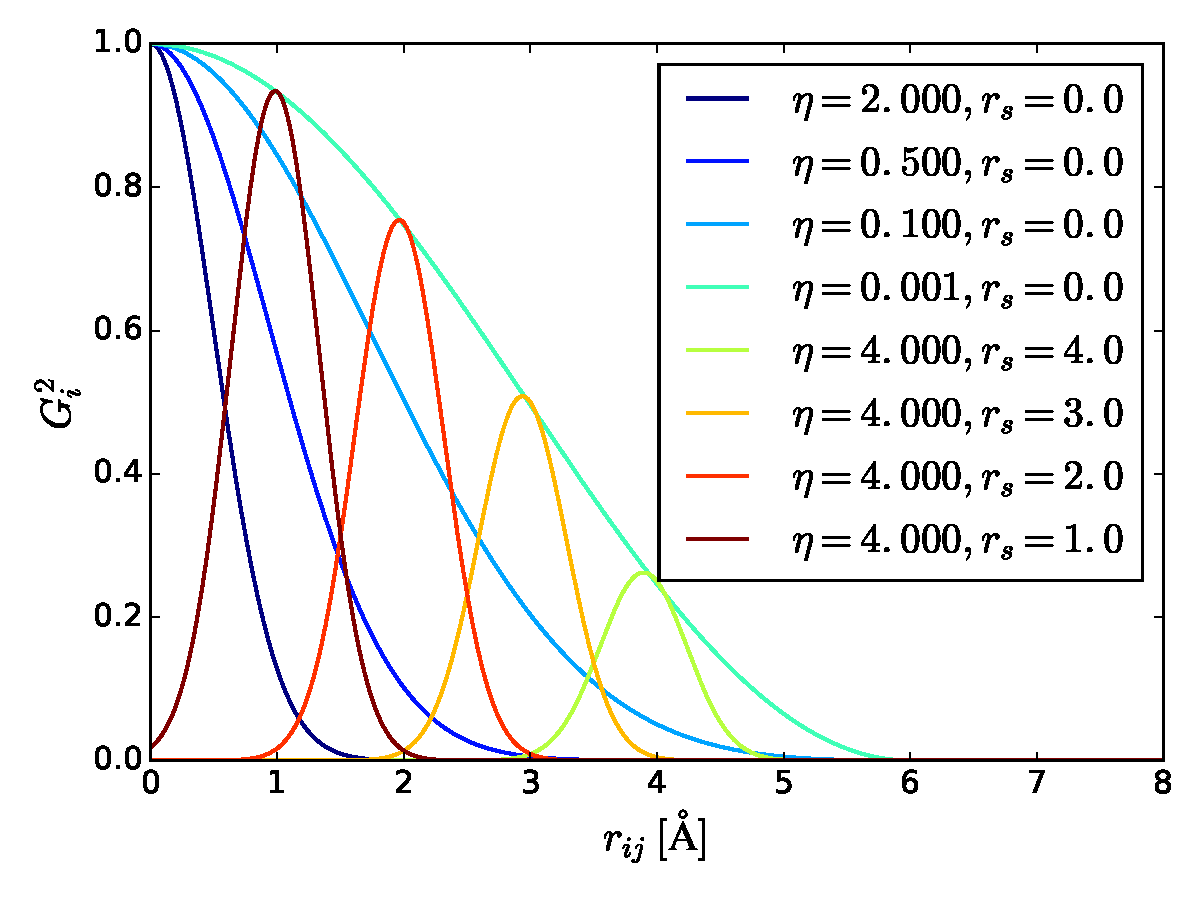
\includegraphics[width = 0.7\linewidth]{Figures/Implementation/radialParams.pdf}
  \caption{Example of an initial radial symmetry function set. The parameters $\eta$ and $r_s$ are varied to 
  probe the radial arrangement of neighbouring atoms.
  All symmetry functions have the same cutoff $r_c = 6.0$. 
  $r_{ij}$, $r_s$ and $r_c$ are in units of $\SI{}{\angstrom}$, while $\eta$ have units $\SI{}{\angstrom}^{-2}$.}
  \label{fig:radialParams}
\end{figure}

\subsubsection{Angular symmetry functions}
A set of initial angular symmetry functions can be made in a similar way. 
The angular distribution of neighbours is probed by varying $\zeta$ and $\lambda$ at differing radii, i.e.\ for 
several values of $\eta$ and/or $r_c$. 
We have found from empirical investigations that fixing $\eta$, while varying $r_c$ yield the best results. 
In contrast to the radial parameters, the set of $\zeta$ parameters should not be equidistant. Instead, the values of $\zeta$
should increase exponentially to ensure that the symmetry functions are sufficiently dissimiliar, i.e.\ to \textit{avoid
strong correlations} (discussed further below).  An example is shown in \autoref{fig:angularParams}. 
\begin{figure}
\centering
  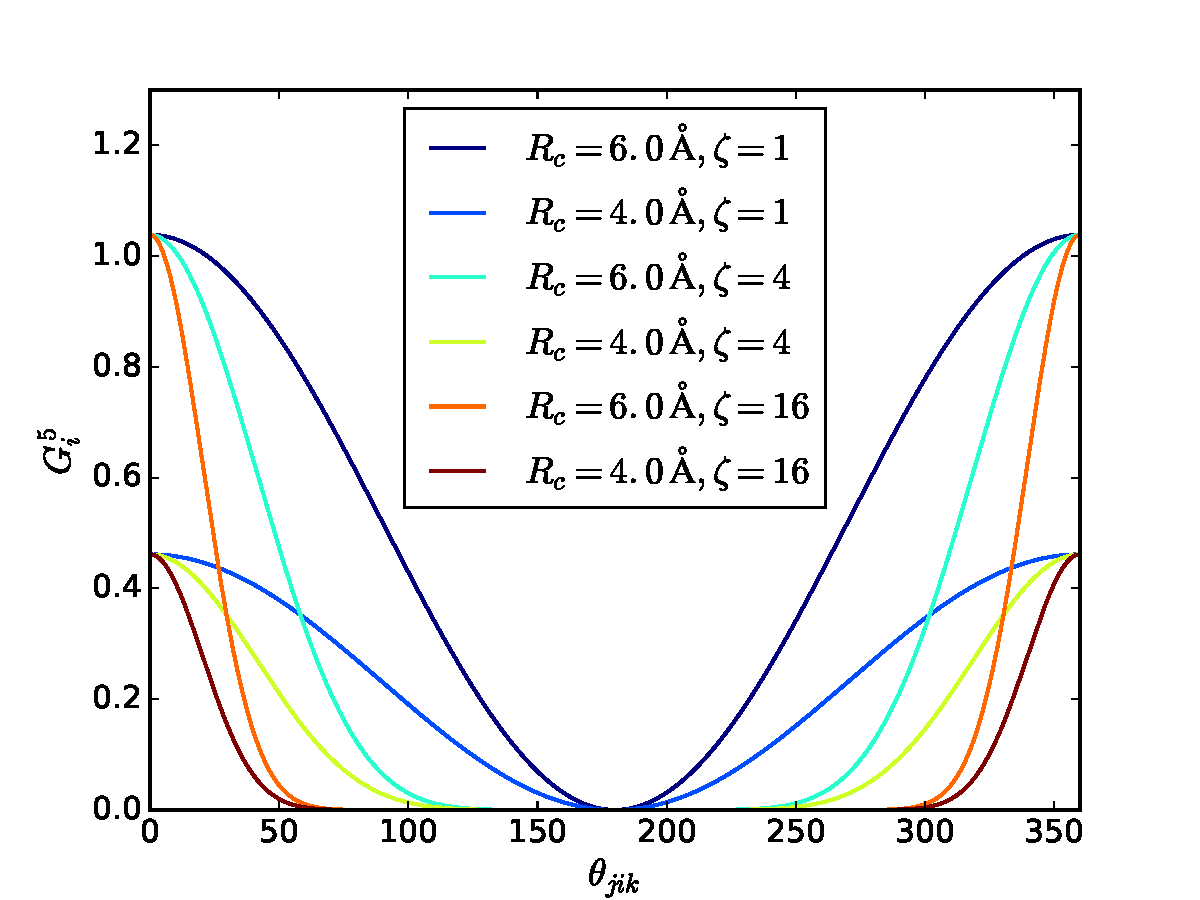
\includegraphics[width = 0.7\linewidth]{Figures/Implementation/angularParams1.pdf}
  \caption{Example of an initial angular symmetry function set
  with $\eta = \SI{0.01}{\angstrom}^{-2}$ and 
  $\lambda = 1$. A corresponding set of functions with $\lambda = -1$ should also be added to make the set more complete. 
  The $\zeta$ parameter is increased in a non-linear way to avoid excessively overlapping functions. }
  \label{fig:angularParams}
\end{figure}

\subsubsection{Number of symmetry functions}
How many symmetry functions should the initial set consist of?
There is a trade-off between the ability of the symmetry function set to cover the configuration space and 
the efficiency of the calculation of the NN energy output. The key is to select enough functions to capture 
all regions of configuratiton space without having any redundancies. 

Further, the number of functions must be large enough for the NNP to be able to distinguish distinct atomic structures that
should yield different total energies. This distinction is more difficult for configurations of a large number of atoms, because
e.g.\ removing one atom from an atomic environment containing 100 atoms only results in a small relative 
perturbation of the symmetry function values. Thus, we should obtain information on how many input atoms 
the eventual NNP is expected to experience in simulations. 

In our case this is an easy task: We simply run MD simulations 
of the system under investigation with the empirical potential to be fitted, and measure coordination numbers. When the 
target potential is unknown, the information can be extracted from empirical knowledge of the system. The number of 
neighbouring atoms will obviously depend on the force cutoffs being used. 

One could immidiately conclude that we
should have at least as many radial and angular functions as there are atomic pairs and triplets respectively, but this is overkill
considering that each one is a function of \textit{all} the atoms inside the cutoff sphere.
From experimenting, we have found that a rule of thumb is to use at least as many radial symmetry functions
as the mean number of expected neighbours. The number of angular symmetry functions should in general be larger because
there are more atomic triplets than pairs for a given ensemble of atoms.  


\subsection{Adjusting the set} \label{sec:adjustSymmSet}
When the initial set is assembled, we carry out various analyses to investigate whether our chosen symmetry functions 
adequately probe the configuration space defined by the data set. There are two requirements
that serve as the guiding principles for the analyses.

\subsubsection{For each symmetry function, the range of function values should be as large as possible}
Each symmetry function
assigns \textit{one} numerical value to each training example. If the range of a symmetry function is too small, 
the difference between the function values for distinct structures will also be small. Consequentially, 
the NN will try to assign substantial energy changes to tiny changes in the symmetry function, which 
can lead to numerical instability. 

This can be avoided by analyzing the distribution of values of each symmetry function on the data set. If the difference 
between the maximum and the minimum function value is below a certain threshold
the symmetry function should be removed or its parameters adjusted. Specifically, 
symmetry functions which have a value of zero for all configurations should be avoided, as these will not contribute
to the description of the chemical environments. 

\subsubsection{The set of values of two different symmetry functions on a given data set should not be strongly correlated}
If there is a large correlation, the two symmetry functions are almost linearly dependent, 
and we have a redundancy of information. Consequentially, one of them should be removed, or the parameters adjusted
to decrease the correlation. Removing functions in this way contributes to keeping the symmetry function set as 
small as possible.

To demonstrate how the correlations can be calculated, we remember that in 
\autoref{sec:training} the data set was represented as a matrix X, where
each row is a training example, in this case the values of all the symmetry functions for a single atomic configuration.
We can calculate the correlations between each pair of symmetry functions with the \texttt{NumPy} method \texttt{corrcoef}, 
\begin{minted}{python}
  R = np.corrcoef(np.transpose(X))
\end{minted}
The data set matrix $X$ is transposed because \texttt{corrcoef} expects each \textit{row} to represent all the samples of one
variable (function), while each \textit{column} is a single observation of all the variables.
A matrix $R$ is returned where the $(i,j)$-th element is the Pearson correlation coefficient between 
symmetry function $i$ and $j$,
\begin{equation}
 R_{ij} = \frac{C_{ij}}{\sigma_i\sigma_j}
\end{equation}
where $C$ is the covariance matrix and $\sigma_i$ is the standard deviation of the values of symmetry function $i$ for 
the whole data set. Pair of functions which are strongly correlated can thus be identified and altered.




\section{Setting hyperparameters} \label{sec:settingHyperParams}
In \autoref{sec:training} and \autoref{sec:optimization} we presented the theory on how a MLP is trained 
by optimizing the weights and biases using an optimization algorithm of choice. 
At the end of \autoref{sec:symmetryFunctions}, we briefly mentioned that a number of so-called hyperparameters must be set
prior to the actual weight optimization, such as the size of the network. 
Choosing hyperparameter values can be treated as a
kind of \textit{model selection}. One set of parameters defines one model, and the goal is to pick the most appropriate 
among a family of such models. The choice can have significant impact on the quality of the fit. 

We distinguish between two kinds of hyperparameters: those that specify the structure of the 
network itself, and those that determine how the network is trained. 
The first type contains parameters that are an integral part of the NN and must be included in the evaluation of the eventual NNP, 
while the second are parameters that are only used during training. The former includes the symmetry function parameters
and any other parameters related to transformations of the input data, the number of layers and nodes, and the choice of 
activation function(s). The second includes 
the learning rate, the mini-batch size, the number of training iterations, the choice of loss function and any additional 
parameters associated with the optimization algorithm and weight initialization.

\noindent In this section we will discuss common techniques for setting hyperparameters. 

\subsection{Preconditioning the input data} \label{sec:transformInputData}
As stated in \autoref{sec:adjustSymmSet}, the individual symmetry functions may have very different ranges of values. 
For a given configuration, each node in the first hidden layer receives as input a weighted sum of all the symmetry function values.
Symmetry functions with large absolute values will have a signicantly stronger impact on the output of these nodes than 
functions with small absolute values. Consequentially, the areas of configuration space covered by the latter functions
may take a longer time for the NN to learn. The importance of the different symmetry functions can be balanced
by normalizing the values of each symmetry function $G_s$  \cite{Behler15}, 
\begin{equation}
 G_{i,s}^\mathrm{norm} = \frac{2(G_{i,s} - G^{\min}_s)} {G^{\max}_s - G^{\min}_s} - 1
 \label{scalingInputData}
\end{equation}
where $G_{i,s}$ is the value of symmetry function number $s$ in the $i$-th training example% 
\footnote{Corresponding to element $X_{ij}$ of the input data matrix.}, and
$G_s^{\min}$ and $G_s^{\max}$ are the smallest and largest values of function $G_s$ in the data set respectively.

Further, convergence is usually faster if the average of each input variable to a NN over the 
data set is close to zero \cite{LeCun12}.
This is because the update of a weight to a node in the first hidden layer is proportional 
to $\delta y_0 = \delta G_s$ \eqref{weightUpdate} where $\delta$ is the error of the node,
and $y_0 = G_s$ is the value of an input node. 
Since all the input values $G_s$ are always positive, the weight updates will all have the same sign, namely $\mathrm{sign}(\delta)$. 
As a result, these weights can only increase or decrease \textit{together} for a given input vector, leading to slow convergence.
The mean of each symmetry function can be shifted to zero by subtracting the mean $\overline{G}_s$ over the data set from 
all function values,
\begin{equation}
 G_{i,s}^\mathrm{shift} = G_{i,s} - \overline{G}_s =  G_{i,s} - \frac{1}{N}\sum_{j=1}^N G_{j,s}
 \label{shiftInputData}
\end{equation}
where $N$ is the number of training examples. Note that scaling \eqref{scalingInputData} and shifting \eqref{shiftInputData}
can also be combined. 

For reasons outlined in \autoref{sec:hyperParamsActFunctions},
another operation that can speed up training is variance scaling \cite{LeCun12}.
This is combined with shifting of means, such that each symmetry function e.g.\ has zero-mean and unit-variance,
called \textit{standardization},
\begin{equation}
 G_{i,s}^\mathrm{stand} = \frac{G_{i,s} - \overline{G}_s}{\sigma_s} 
 \label{scaleVariance}
\end{equation}
where $\sigma_s$ is the standard deviation of symmetry function $G_s$. 

\subsubsection{Convergence speed vs evaluation speed}
We have seen that a number of operations can be performed on the input data to speed up the fitting process.  
Note that the these can be applied to the target values as well %  
\footnote{The observations on scaling and shifting of input variables are valid for most 
types of input and output data. Scaling of target values are more important 
for classification, where the output is binary (e.g.\ \{-1,1\}), than for regression.}. However, for the construction of NNPs, 
the convergence speed is not a main issue. In contrast to e.g.\ object recognition with deep convolutional networks, where
often thousands of NN parameters are needed \cite{LeCun99}, NNPs usually require only up to a few hundred weights. Even though 
the data set to be fitted can be quite extensive, the duration of the training is rarely more than 30 minutes to 1 hour before 
an acceptable error is achieved.

Further, there is a trade-off between the convergence speed and the evaluation speed of the resulting NNP. 
As for the symmetry transformations, the above operations become an integral part of the NNP, and must be performed 
when the potential is to be applied in simulations. Considering the importance of computational performance in MD simulations,
an increase in training speed at the cost of evaluation speed is not to be preferred, as long as the \textit{quality} of the fit 
is not influenced by these operations. This will be investigated in \autoref{sec:SiPotentialResults}. 



\subsection{Activation functions and weight initialization} \label{sec:hyperParamsActFunctions}
In \autoref{sec:activationFunctions} we stated that the sigmoid \eqref{sigmoidActivationFunction} and 
the hyperbolic tangent \eqref{tanhActivationFunction} are the most common activation functions for regression
with neural networks. They are both \textit{saturating} functions because they map real numbers into the restricted intervals 
[0,1] and [-1,1] respectively. This property keeps the outputs of neurons from diverging, but it also contributes to 
the problem of \textit{vanishing gradients}. We know from \autoref{sec:backprop} that
weight updates are proportional to the derivatives of neuron outputs $y$ \eqref{backprop},
\begin{equation}
 y^\prime = f^\prime(u)
\end{equation}
where $f$ is the activation function and $u$ is the input. 
We see from \autoref{fig:SigmoidActivationFunctions} that the sigmoid and hyperbolic
tangent have very small gradients for all inputs except those in the small non-linear region around zero, corresponding 
to about [-4,4] and [-2,2] respectively. 
Large positive or negative inputs therefore result in vanishing gradients and tiny updates, slowing down learning. 

Note that saturation occurs naturally if a network is absolutely correct on all training examples and 
hence does not need to change its weights. However, premature saturation is a common problem in neural network training, and may slow
down or even prevent learning. It can be avoided by restricting neuron inputs $u$ to the non-linear region of their 
activation functions, with the help of two different procedures. 

First, scaling/standardization (\autoref{sec:transformInputData}) of the input data helps to achieve this for
the neurons in the first hidden layer. The distribution of inputs to the next layer depend on the choice of activation function, and 
here the sigmoid and the tangent differ: The former have mean 1/2, while the latter is symmetric around zero. 
Obviously, zero-mean is preferred, as any positive or negative bias inevitably have a larger risk of pushing the activations 
towards saturation. Thus, the hyperbolic tangent is generally preferred over the sigmoid, which have also been demonstrated 
empirically \cite{Karlik11,Glorot10}. 

Secondly, since the weights and biases also contribute to the sum $u$, they should be initialized as small numbers centered around zero. 
A common scheme is to 
set all biases to zero, and assign weight values according to some probability distribution with zero-mean and 
a suitable (small) variance. Assuming standardized input data, 
a frequently used heuristic is to initialize the weights $W_{ij}$ at each layer by 
\cite{Bengio12,LeCun12},
\begin{equation}
 W_l \in U\left[-\frac{1}{\sqrt{n_{l-1}}}, \frac{1}{\sqrt{n_{l-1}}}\right]
\end{equation}
where $U[-a, a]$ is the uniform distribution in the interval $[-a,a]$, $n_l$ is the size of layer $l$, and 
$W_l$ is the weight matrix connecting layer $l-1$ and $l$. 
A disadvantage of this method is that a layer-dependent weight variance might result in saturated upper layers 
if the layer size changes through the network.  
Glorot and Bengio \cite{Glorot10} have suggested a modification of this scheme that gives rise to a variance that 
is equal through the whole network. The idea is to 
conserve the input signal when propagated through the network by preventing it from shrinking or growing too much,  
\begin{equation}
 W_l \in U\left[-\frac{\sqrt{6}}{\sqrt{n_{l-1}+n_{l}}}, \frac{\sqrt{6}}{\sqrt{n_{l-1}+n_{l}}}  \right]
\end{equation}
This is only valid for an activation function that is symmetric and has a unit derivative at 0 ($f^\prime(0) = 1$), i.e.\ only 
for the hyperbolic tangent. Further, all input variables are assumed to have the same variance.




\subsection{Network architecture and overfitting} \label{sec:overfitting}
There is no standard and accepted method for finding the optimal size of a NN for a specific data set. 
In this work, the input layer is a set of symmetry functions that acts as descriptors of atomic configurations.
The size of this set thus decides the number of neurons in the input layer, which is discussed in \autoref{sec:initialSymmSet}. 

The output layer only consists of \textit{one} neuron that represents the total energy of an atomic 
configuration. Additionaly, we can have an arbitrary number of hidden layers and nodes. 
Many nodes means many parameters that can be tuned to the data set, resulting in a better fit.
However, if the number of neurons is too large, the network will \textit{overfit} the reference data. 
In this case, the network fits the data set very well, but interpolation between the training points is poor. Thus, 
the NNP becomes less predictive, and will not perform well in simulations.

\textit{Regularization} is a number of processes from statistical learning theory that deals with ill-posed optimization
problems and overfitting. A well-known method to prevent the latter is \textit{early stopping}. 
Here, the reference data is randomly split into 
a \textit{training set}, which is employed for the optimization of the weights, and a \textit{test set}, whose error is monitored
during the fit but which is not used to adjust the weights. A typical test set size is 10-20 \% of the reference data.
If the errors of these two sets are similar, we know that the NN
generalizes to data that has not been used in its training. On the other hand, if the test set error is significantly larger
than the training set error, overfitting is occuring, and training should be stopped. The most commmon error measure
is the root-mean-square-error (RMSE), 
\begin{equation}
 \mathrm{RMSE}(\mathrm{NN}) = \sqrt{\frac{1}{N}\sum_{i=1}^N (Y_i - y_i)^2}
\end{equation}
where $y_i$ is the NN prediction and $Y_i$ is the reference value, as before. 
This expression is almost equivalent to the cost function \eqref{quadraticCost} used in the optimation of the NN.

\autoref{fig:overfitting} displays a typical case of overfitting. Here we have sampled a training set 
of 5578 configurations and energies from a Si Stillinger-Weber simulation. Then, we have trained two NNs 
with the same set of hyperparameters, first on the full training set a), then on only the first 300 training examples b).
The test set is identical in both cases. We observe that the training set error and the test set 
error are very similar in a), while in b) there are a significant deviation between the two. The latter is clearly a case 
of overfitting caused by an incomplete training set.  
\begin{figure}
\centering
  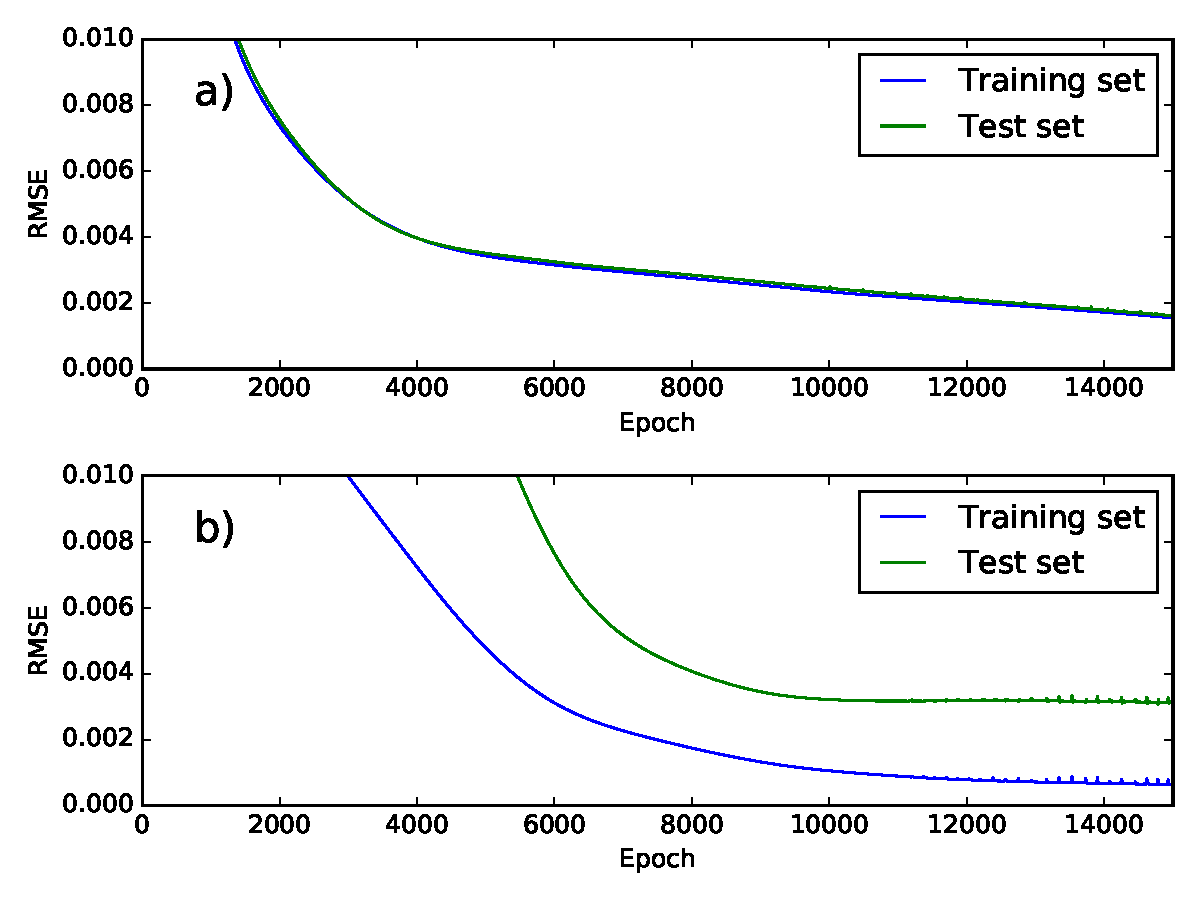
\includegraphics[width = 0.8\linewidth]{Figures/Implementation/overfitting.pdf}
  \caption{Demonstration of overfitting. Both figures show the RMSE of a NN evaluated on both the training set and 
	   the test set. The training set consists of 5578 training examples from a Si Stillinger-Weber simulation.
	   In a), the NN has been trained on 
	   the whole training set, while in b) only the first 300 training examples were used. The test set is 
	   identical in both cases. We clearly see that overfitting occurs in b).}
  \label{fig:overfitting}
\end{figure}

The early stopping method automatically determines another hyperparameter, namely the number of epochs to train. 
However, it does not give us the optimal NN architecture. Overfitting can also be caused by an incomplete data set, 
and reducing the number of neurons is not necessarily the best solution. Often, more data should be added instead, 
and the current NN size may fit the extended data set better. 

Early stopping is in other words not necessarily a reliable method to decide if a NN is of a suitable size or not, 
but primary a tool to prevent overfitting. 
The only way to find the optimal architecture is by training several networks of different sizes and choose the one that yields
the lowest error while simultaneously not overfitting. The problem with this strategy is that the possibilities are very many. 
We can however make a few observations to narrow down the search. 
According to Larochelle et al.\ \cite{Larochelle09}, having the same number of nodes in each hidden layer givse the best results. 
Further, in the literature we have studied concerning NNPs, e.g.\ \cite{Behler07,Raff05,Witkoskie05}, 
only one or two hidden layers are used, and we know from the universal approximation theorem (\autoref{sec:whyMLP})
that one hidden layer is sufficient to represent any function. For typical AI tasks, deeper architectures are required 
\cite{Bengio07}, but in this thesis we will limit ourselves to maximum three hidden layers. 

\subsubsection{Other regularization teqhniques}
There exist other regularization techniques in addition to early stopping that reduce overfitting. 
\textit{Weight decay} or \textit{L2 regularization} adds an extra term to the cost function, called 
the \textit{regularization term}, which is the sum of squares of all weights in the network \cite{Krogh1992},
\begin{equation}
 \Gamma = \Gamma_0 + \frac{\lambda}{2N}\sum_w w^2
\end{equation}
where $\Gamma_0$ is the original, unregularized cost function, $N$ is the size of the training set and 
$\lambda$ is the \textit{regularization parameter}. The idea is to penalize large weights, and the modified 
cost function can be viewed as a compromise between finding small weights and minimizing the original cost function.
The parameter $\lambda$ determines the relative importance of these two elements. 
Keeping the weights small makes the output of the NN more resistant to outliers and noise in the input data, thus
putting more emphasis on the frequent input patterns. 
The hope is that this will force the NN to see ''the bigger picture'', 
and hence generalize better. 

Another more recent technique to reduce overfitting is \textit{dropout} \cite{Srivastava14}. Here, the key idea 
is to randomly remove neurons from the NN during training. This prevents nodes from co-adapting too much and 
also decreases the size of the network. We will not go into further detail on this subject here. 

We have decided to employ early stopping only to prevent overfitting, as more training data is easily obtained from MD 
simulations with empirical potentials, making overfitting not a pressing issue. 


\subsection{Optimizer parameters}
There are several optimization hyperparameters that need to be decided, namely the learning rate, the mini-batch size
(if we employ mini-batch gradient descent) and parameters inherent to the update rule of choice. 
We restrict ourselves to optimization algorithms that use adaptive learning rates, thus only an \textit{initial}
learning rate needs to be set. According to Bengio \cite{Bengio12}, a default value of 0.01 is appropriate, but 
a set of different values should be tested (\autoref{sec:optimizingHyperparameters}), 
as the optimal value may depend strongly on the data set and the NN architecture. 

In \autoref{sec:gradientDescentVariants} we discussed different types of gradient descent learning, and 
declared that mini-batch gradient descent usually is the preferred scheme. The main reason for this is that data sampled from molecular 
dynamics simulations, even with a good sampling algorithm, often contain redundant information: many configurations 
are similar because the system tends to stay near equilibrium%
\footnote{This is of course not the case if the intended
application of the NNP is for non-equilibrium molecular dynamics.}. Thus, batch learning, where the weights are updated 
only after the complete training set have been fed to the network, is wasteful because it recomputes nearly the same outputs
several times before updating the weights \cite{LeCun99}. 

However, to employ mini-batch gradient descent, we have to determine another 
hyperparameter, namely the mini-batch size. According to Bengio \cite{Bengio12}, 32 is a good default value. Further, it is argued 
that the mini-batch size should mainly impact the training time and not so much the eventual error of the fit.
Therefore, we will not discuss this parameter any further, and refer to \autoref{sec:optimizingHyperparameters} for a discussion
on how to optimize hyperparameters.

Some optimizers, like Adam \eqref{adamUpdateRule}, contain other hyperparameters in addition to a learning rate.  
Each of these algorithms has a set of default values that are well justified, and we have decided not to alter these. 

\subsection{Cost function} \label{sec:hyperParamsCostFunction}
We only use the mean-square error \eqref{quadraticCost} as a cost function in this thesis. 
An obvious weakness of using this is that we only fit the reference function Y (the potential) itself, 
not its gradient $\mathrm{Y}^\prime$ (the forces). If a small error is achieved for the potential fit, we would expect that 
the error is low also for the gradient, but this is not assured. The force error is of vital importance, considering 
that the forces determine the dynamics of a simulation. 

Pukrittayakamee et al.\ \cite{Pukrittayakamee09} have suggested an extension to the standard mean-square error, that 
enables simultaneous fitting of both a function and its gradient (the CFDA algorithm). 
This is achieved by penalizing both the error 
in the potential and in the forces, and has also been employed by Behler in a modifed form \cite{Behler15},
\begin{equation}
 \Gamma = \frac{1}{N}\sum_{i=1}^N \biggr[(E_i^{\mathrm{ref}} - E_i^{\mathrm{NN}})^2 + 
 \frac{\beta}{3N_i}\sum_{j=1}^{3N_i} (F_{i,j}^{\mathrm{ref}} - F_{i,j}^{\mathrm{NN}})^2 \biggr]
 \label{CFDA}
\end{equation}
As before, the first sum is over $N$ training examples, where $E_i^{\mathrm{NN}}$
is the energy prediction of the NN for training example $i$ and $E_i^{\mathrm{ref}}$ is the $i$-th reference energy. 
For training example $i$, there are $3N_i$ force components corresponding to a configuration of $N_i$ atoms. We have that
\begin{subequations}
\begin{align}
 F_{i,j}^{\mathrm{ref}} &= \frac{\partial E_i^{\mathrm{ref}}}{\partial r_{i,j}} \label{forcesCFDA1} \\
 F_{i,j}^{\mathrm{NN}} &= \frac{\partial E_i^{\mathrm{NN}}}{\partial r_{i,j}}
 \label{forcesCFDA2}
\end{align}
\end{subequations}
where $r_{i,j}$ is the $j$-th position component of training example $i$. The NN still has only one output neuron
that represents the total energy of a training example. The forces (\ref{forcesCFDA1},~\ref{forcesCFDA2}) are computed as
described in \autoref{sec:symmAndForces}.
To minimize \eqref{CFDA} we need its gradient, which means that second derivatives of the NN 
are required. This seems like a daunting task, but can be performed quite easily in TensorFlow. 
The command
\begin{minted}{Python}
 tf.gradients(y, x)
\end{minted}
computes the symbolic partial derivative of TF tensor \texttt{y} with respect to TF tensor \texttt{x}. In general, each tensor 
in a computational graph can be differentiated with respect to any other tensor in the same graph. 

We will not go into further detail on how the CFDA algorithm can be embedded in the training process. 
Computing second derivatives of the NN during training are computationally demanding, and since we have obtained 
good results without directly fitting the forces as well, we will stick to the ordinary mean-square cost function. 



\subsection{Hyperparameter space exploration} \label{sec:optimizingHyperparameters}
In this section we have discussed various tricks of the trade regarding hyperparameters for training neural networks. 
We realize that there are a substantial number of choices to be made, corresponding to a large parameter space, and 
that many (if not all) of these choices are ipmortant for a successful outcome. Even though the above discussions narrows down the search 
for suitable hyperparameters, it is still a difficult task. 

An alternative is to treat hyperparameter selection as an optimization problem, i.e.\ to train the NN for many different 
parameter sets and choose the set that yields the best fit. To perform this task, it is common to split the data set 
into three parts: A training set, a test set, and a \textit{validation set}. The first two sets have the same 
purpose as before (\autoref{sec:overfitting}), while the validation set is used to test the model during hyperparameter 
optimization. This is done so that we do not overfit the hyperparameters to the test set, which is only used to assess 
the performance of the final NN model of choice.

In the following we will describe various hyperparameter optimization schemes. 

\subsubsection{Coordinate descent}
In coordinate descent, we keep all hyperparameters fixed except for one. Then we adjust this single parameter and train the NN
for each value to minimize the validation error  .

\subsubsection{Grid search}
Grid search is the most simple and brute-force way to optimize hyperparameters: We simply try every hyperparameter setting 
over a specified range of values and choose the set with the lowest validation error. This is obviously very computationally 
expensive, and is often infeasible in practice. 

\subsubsection{Random search}
Instead of performing a grid search, we can sample the hyperparameter space randomly. This is usually a better option because 
a grid search may take a long time to reach sensible combinations of parameters, and because only a few parameters
tend to be vital for the result. 

\subsection{Summary}
We have in this section discussed all hyperparameters that needs to be chosen to construct a NNP. 
It must be stressed that many of the above recommendations for hyperparameter choices may not be suitable 
for all problems, and that the only way to find unbiased, optimal values is by an extensive search 
in hyperparameter space. However, the quality of the fit may be insensitive to some parameters, which makes their 
determination less important. 
We refer to \autoref{sec:SiPotentialResults} for a demonstration on how 
a combination of qualitative arguments and optimization can be performed to find suitable parameters 
for a specific case. 



\section{Applying the neural network potential} \label{sec:applyingNNP}
The quality of a NNP is measured by its test set error, but that does not necessarily mean it performs 
well in MD simulations. To properly validate the NNP, we have to apply it in simulations, measure thermodynamic quantites, 
and see if we reproduce known, experimental results. 

In this thesis we use the TensorFlow (TF) Python API to train neural networks, while LAMMPS, written in C\texttt{++}, is
employed to run MD simulations for speed purposes. 
We therefore need a way to transfer the NNP from Python to C\texttt{++}. 

There are built-in functions in TF that automatically saves computational graphs (architecture of network plus
nodes for training) and variables (weights and activation functions) as binary files.
These files can then be read and the NN evaluated using the TF C\texttt{++} API. This API is however quite under-developed
and the documentation is very sparse. 

Another alternative that we have developed is to manually save the weights and biases
as a text file, along with the necessary hyperparameter values, such as choice of activation function and 
symmetry function parameters. This file 
can then be used to reconstruct the NN in the same way that it is made in Python: by representing
the connection weights between layers as matrices and the biases as vectors 
(\autoref{sec:MLPmodel} and \autoref{sec:TensorFlowCreatingNN}). 
The activation functions must be implemented manually. A linear algebra library can
be utilized for speed and simplicity; we have chosen to use Armadillo%
\footnote{\href{http://arma.sourceforge.net/}{Armadillo}}. 

To find out which alternative that is the most computationally efficient, we compare the 
time usage between evaluating a NN with TensorFlow and Armadillo in C\texttt{++}. We also compare with TF in Python to 
investigate if any differences between TF and Armadillo in C\texttt{++} is caused by an under-developed C\texttt{++} TF API, or 
if the cause is inherent to the TF implementation of neural networks.
The evaluation time 
is measured for a range of different NN sizes, and for each size an average of 50 evaluations have been computed.
The results are shown in \autoref{fig:timeComparisonEvaluateNetworkTotalScatter}.
\begin{figure}[t]
\centering
  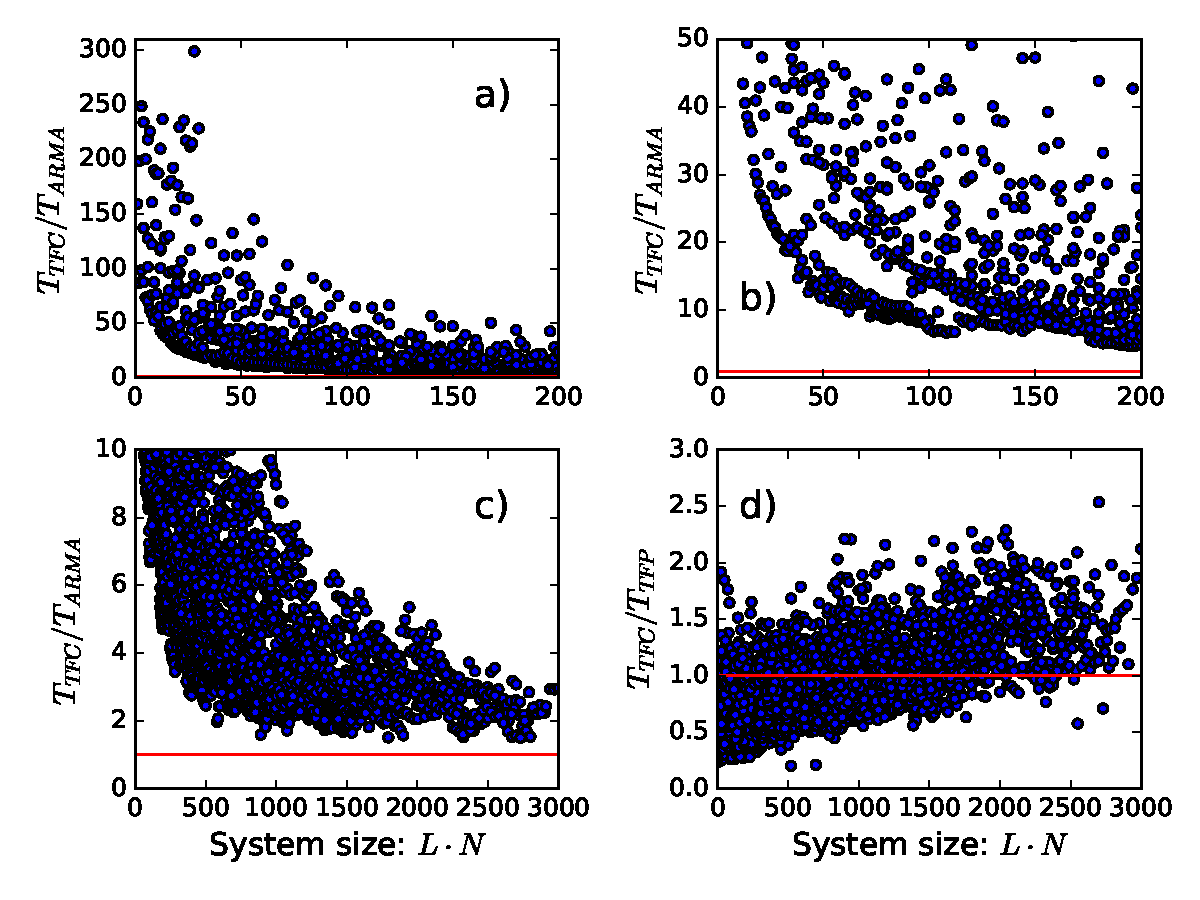
\includegraphics[width = 0.9\linewidth]{Figures/Tests/timeComparisonNetworkNew.pdf}
  \caption{Scatter plot of time usage when evaluating untrained NNs with random weights and sigmoid activation functions
	   using the TF Python API ($T_{\mathrm{TFP}}$), the TF C\texttt{++} API ($T_{\mathrm{TFC}}$) and Armadillo ($T_{\mathrm{ARMA}}$). 
	   $L$ is the number of hidden layers, $n$ is the number of nodes in each hidden layer. All the NNs
	   have one input and one output. The time has been calculated by averaging over 50 evaluations
	   for each NN architecture.}
\label{fig:timeComparisonEvaluateNetworkTotalScatter}
\end{figure}

Figure a) and b) display the ratio $T_{\mathrm{TFC}}/T_{\mathrm{ARMA}}$ for NN sizes up to 200, the former with all data points 
visible, while the latter is zoomed in to give a more detailed picture. We observe that the time difference is huge 
for small networks, and that even for NNs of size 200 the ratio is still about 5. From c), we decude that the ratio seems to converge 
to 1 for large networks, but the convergence rate is surprisingly low. 
As we see from d), the performance of the built-in TF functions is similar 
in C\texttt{++} and Python, thus the time deviation can not be caused by an under-developed C\texttt{++} API. 

One reason for this phenomenon may be that the \texttt{Session} environment in TF has a lot of overhead. 
Further, a NN size of 3000 is small compared to e.g.\ state-of the art convolutional networks, which are usually trained with GPUs. 
Considering that we will not need NNs containing more than 100-200 neurons, a manual implementation of NNs with Armadillo 
is definitively the best choice. 

\section{Summary}
In this chapter we have discussed the details of the NNP construction steps, specifically how to sample an adequate training set,
how to determine hyperparameters, and how to apply a NNP in simulations. 
The construction process will be exemplified 
in two specific cases. In \autoref{sec:LJValidation}, we will train a NN reproduce the truncated and shifted 
Lennard-Jones potential \eqref{shiftedLJ}. The quality of the fit will be analyzed, but the NNP will not be applied 
in simulations. In \autoref{sec:SiPotentialResults}, we will construct a NNP for solid-state Si and apply it in simulations 
to measure the radial distribution function and various mechanical properties. 




\chapter{Lennard-Jones validation} \label{sec:LJValidation}
As a first test of our implementation of the NNP construction process, we train a neural network to reproduce 
the truncated and shifted Lennard-Jones potential \eqref{shiftedLJ}. 
The fitting is performed with a NN that has one input and one output, resulting in 
a NNP that computes the potential energy of a central atom $i$ in the presence of a single neighbour $j$ of the same element at 
a distance $r_{ij}$. This one-dimensional NNP does not face the same symmetry issues as its many-dimensional counterpart: 
having only one input removes the problem that the energy should be invariant to the order of atoms, and 
the relative coordinate $r_{ij}$ is invariant to a translation or rotation of a diatomic system. Thus, no symmetry functions 
are needed. 

The configuration space of this NNP is simply $r_{ij} \in [a,b]$, where $a$ and $b$ are the smallest and largest 
interatomic distance respectively that the NNP is expected to experience in a simulation. 
Suitable values of $a$ and $b$ are found by running a MD simulation with the potential that is to be fitted
at the temperature intended for the NNP application of the NNP, and measure the minimum and maximum pair-wise distance. 
To sample this configuration space, we simply draw random numbers from a uniform distribution with $a$ and $b$ as endpoints,
\begin{minted}{Python}
 inputTrain = np.random.uniform(a, b, trainSize)
 inputTest  = np.random.uniform(a, b, testSize)
\end{minted}
while the reference energies are calculated by employing the analytical expression for the target function \eqref{shiftedLJ}. 
The hyperparameters used are listed in \autoref{tab:hyperParamsLJ}. These have not been optimized, but suitable values
have been determined on the basis of the discussion in \autoref{sec:settingHyperParams}. The input data has 
not been transformed in any way. 
\begin{table}[t]
  \begin{center}
    \begin{tabular*}{12cm}{l @{\extracolsep{\fill}} ll}
      \toprule
      Hyperparameters &  \\ 
      \hline
      Network structure & Inputs & 1 \\
      & Outputs & 1 \\
      & Hidden layers & 1 \\
      & Hidden nodes & 10 \\
      & Activation & Sigmoid \\ 
      Training & $a$  & \SI{3.2}{\angstrom} \\
      & $b$  & \SI{8.5125}{\angstrom} \\
      & Training set size & 10000 \\
      & Test set size & 1000 \\
      & Mini-batch size & 200 \\
      & Number of epochs & 5000 \\
      & Optimizer & Adam \\
      & Initial learning rate & 0.001 \\
      & Weight initialization & $U \in [-0.1, 0.1]$ \\
      & Bias initialization & $U \in [-0.1, 0.1]$ \\
      \bottomrule
      \end{tabular*} 
    \end{center}
    \captionsetup{width=12cm}
      \caption {Hyperparameters used in the fitting of the truncated and shifted Lennard-Jones potential \eqref{shiftedLJ}.
		The meaning of each parameter is found in the text. 
                ''Hidden nodes'' signifies the number of nodes in each hidden layer. } 
  \label{tab:hyperParamsLJ} 
\end{table}

After 5000 epochs, we obtain a test set RMSE of 0.896 meV. This is a good result, considering that no hyperparameters 
were optimized. However, fitting a one-dimensional target function is not a great challenge, despite its non-linear behaviour. 
The test set RMSE and the training set RMSE follow each other very closely, and no overfitting occurs. 

\section{Error in configuration space}
It can be useful to visualize the error distribution in configuration space 
by evaluating the trained NN on all data points in in the test set, and compare with the target function, 
\begin{minted}{Python}
...
# evaluate trained network on this interval and find absolute error
inputTest = np.sort(inputTest)
energiesNN = sess.run(NNprediction, feed_dict={x: inputTest})
energiesLJ = LennardJones(inputTest)
energyError = energiesLJ - energiesNN
\end{minted}
where \texttt{x} is a \texttt{tf.placeholder} as described in \autoref{sec:TensorFlowCreatingNN}. 
The absolute error $E_\mathrm{LJ} - E_\mathrm{NN}$ is plotted as a function of distance $r_{ij}$ in \autoref{fig:LJError}.
We notice that the error oscillates around zero, and that the amplitude is larger for smaller distances.
This is in accordance with the observations made in \autoref{sec:samplingAlgorithms}: The regions of configuration space 
where the gradient of the target function is large, is more difficult to fit, and should therefore have a higher density. 
The training set is in this case uniformly distributed, thus the error is larger for small inter-atomic distances where 
strong repulsive forces are at work. Nevertheless, the NN energy prediction follows the shape of the LJ potential very closely
for most values of $r_{ij}$. 
\begin{figure}
\centering
  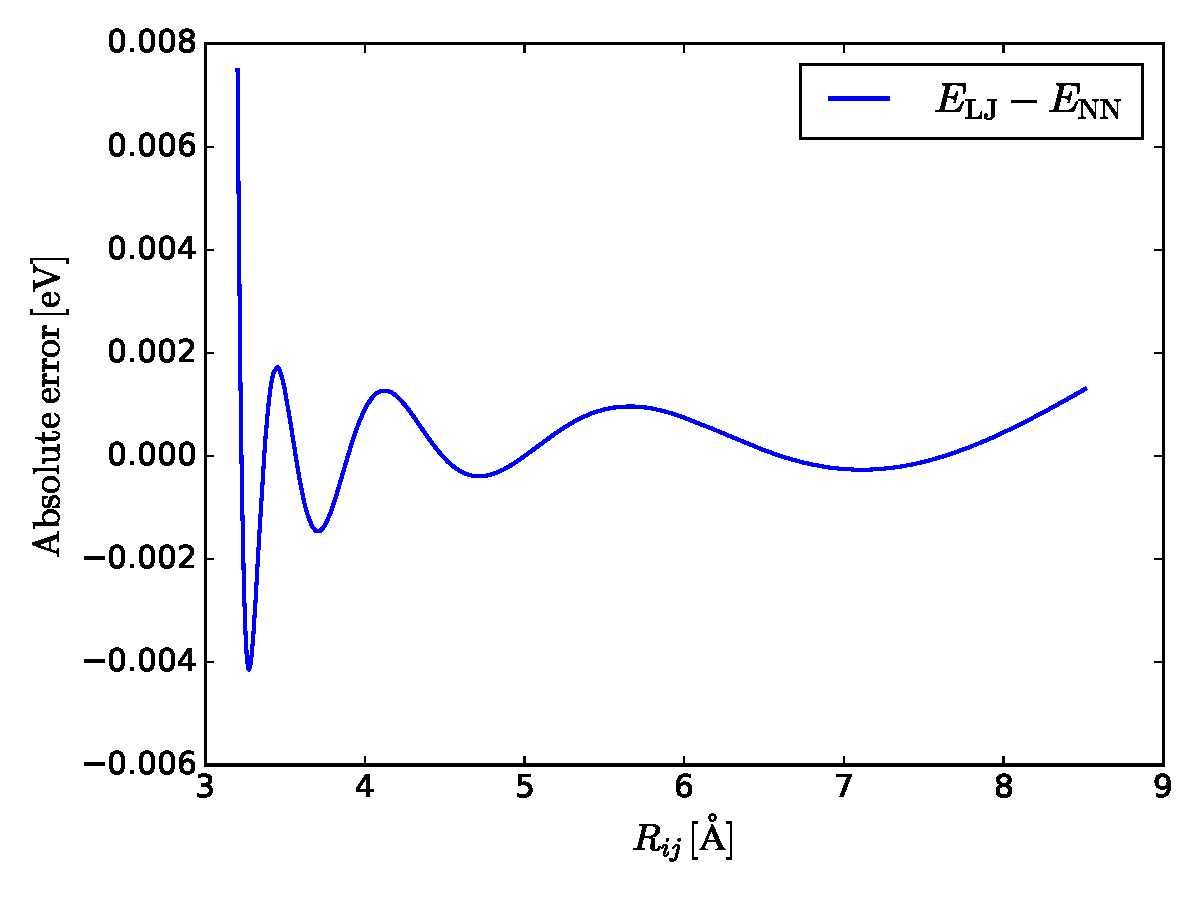
\includegraphics[width = 0.7\linewidth]{Figures/Implementation/LJError.pdf}
  \caption{Absolute error of a NN trained to reproduce the truncated and shifted Lennard-Jones potential \eqref{shiftedLJ}. 
           The plot is as a visualization of the error distribution in the configuration space $r_{ij} \in [a,b]$ 
           defined by the test set. The employed hyperparameters are listed in \autoref{tab:hyperParamsLJ}.} 
  \label{fig:LJError}
\end{figure}

To obtain the forces in a simulation, we must calculate the gradient of the NN. 
In \autoref{sec:hyperParamsCostFunction} we mentioned that a small energy RMSE does not 
necessarily imply a small force RMSE. In this one-dimensional example, it is easy to measure the gradient error. 
This is done in a same manner as for the energy above, except now we are comparing the gradients of the NN and the target function. 
We also calculate the RMSE of the gradient on the test set,
\begin{minted}{Python}
...
derivativeLJ = LennardJonesDerivative(inputTest)

# define a NN gradient operation and differentiate
gradientOP = tf.gradients(NNprediction, x)
derivativeNN = sess.run(gradientOP, feed_dict={x: inputTest} )[0]

gradientError = derivativeLJ - derivativeNN
gradientRMSE = np.sqrt(np.sum(gradientError**2)/testSize)
\end{minted}
We obtain a gradient RMSE of 24.3 meV, which is about one order of magnitude larger than for the function itself. 
This function-gradient RMSE ratio is also reported by others \cite{Natarajan16,Artrith12}. 

The absolute error plot is shown in \autoref{fig:LJErrorDerivative}. 
Again we have an oscillating error over the training interval, but with 
larger amplitudes. The gradient error at $r_{ij} = a$ is about 50 times larger than the energy error at this point, which  
demonstrates the importance of having a higher density of training points in certain regions. 
\begin{figure}
\centering
  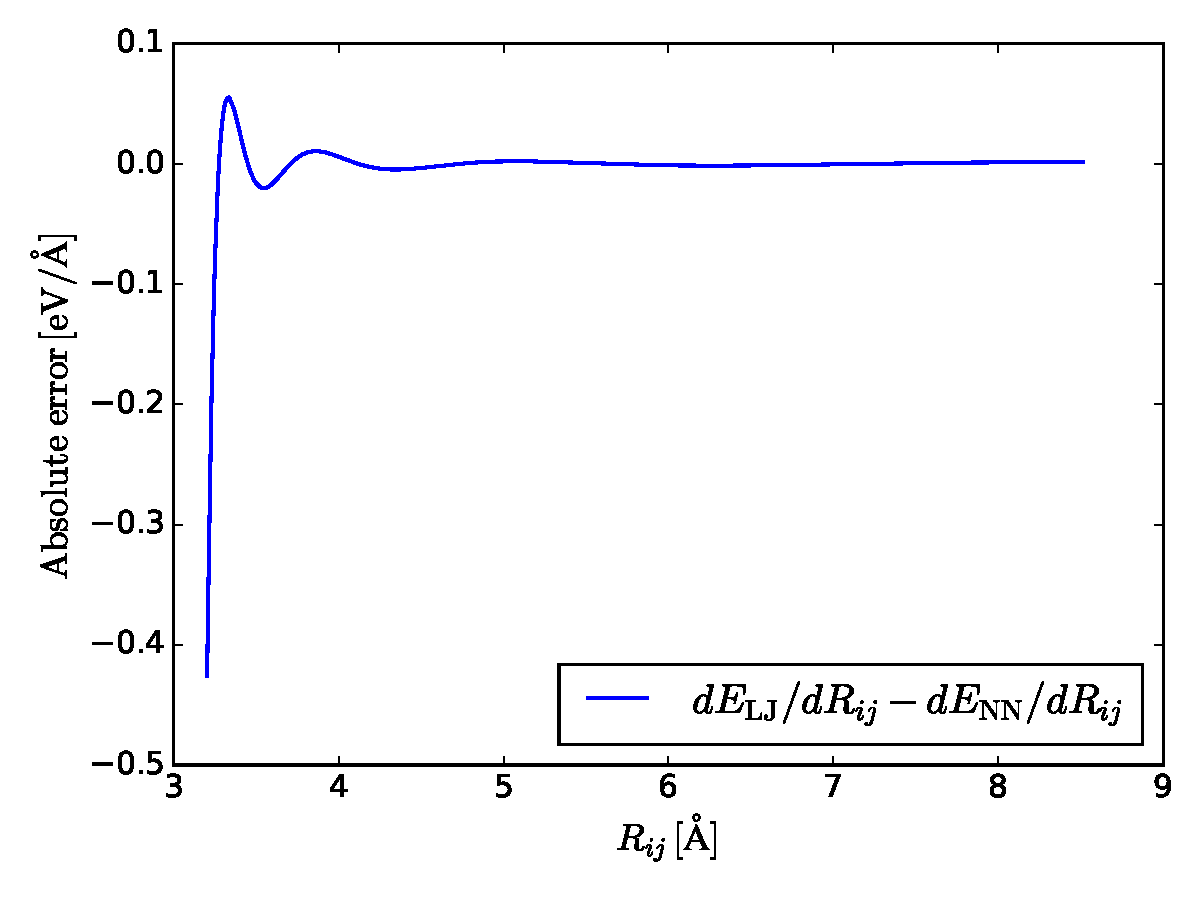
\includegraphics[width = 0.7\linewidth]{Figures/Implementation/LJErrorDerivative.pdf}
  \caption{Absolute error of the gradient of a NN trained to reproduce the truncated and shifted Lennard-Jones 
           potential \eqref{shiftedLJ}. Comparing with \autoref{fig:LJError}, we see that the graph is of the same shape, 
           but with larger oscillations. The employed hyperparameters are listed in \autoref{tab:hyperParamsLJ}. }
  \label{fig:LJErrorDerivative}
\end{figure}




\chapter{Neural network potential for Si} \label{sec:SiPotentialResults}
In this chapter we perform a demonstration of the complete NNP construction process, including 
the Behler-Parrinello method. The goal is construct a potential for solid-state Si by sampling atomic configurations 
and energies from Stillinger-Weber MD simluations. 
The eventual NNP will be validated by computing the radial distribution function and several mechanical properties, and compare
with SW. 

\section{Sampling initial set}
To assemble the initial data set, we need to decide on the specific application of the NNP that we want to develop. 
We choose to construct a potential that can be used to simulate solid-state Si in a temperature range of $T \in [0, 500] \, \mathrm{K}$. 
The system is prepared in a diamond cubic state with a lattice spacing of \SI{5.431}{\angstrom}, which is 
the crystalline structure of Si. We perform several simulations of the microcanocical ensemble with initial temperatures
in the above range and a time step of $\Delta t = 0.001 \, \mathrm{ps}$.
The SW potential is parametrized according to \cite{Stillinger85}, with a force cutoff 
of $r_c = \SI{3.77118}{\angstrom}$. 
Periodic boundary conditions are imposed and the sampling algorithm 
\eqref{samplingAlgorithmModified} is applied in each simulation, resulting in 4406 structures and corresponding energies.
Note that if an \textit{ab inito} NNP is to be constructed, the reference energies must be calculated with a
quantum mechanical method, which is outside the scope of this work.

\section{Initial symmetry function set}
To get an idea of how many symmetry functions that are needed, we run a MD simulation as described above and 
measure the minimum, maximum and average coordination numbers as a function of time, 
\begin{lstlisting}[style=lammps]
# coordination number of each atom
compute neighbours all coord/atom cutoff 3.77118

# global coordination numbers
compute minNeigh all reduce min c_neighbours
compute maxNeigh all reduce max c_neighbours
compute aveNeigh all reduce ave c_neighbours

thermo_style custom step c_minNeigh c_maxNeigh c_aveNeigh 
\end{lstlisting}
After 1e5 time steps, the minimum and maximum coordination number of any atom were 4 and 12 respectively, with an average 
of around 6. Thus, according to the discussion in \autoref{sec:initialSymmSet}, 6-8 radial symmetry functions should be sufficient, 
while the angular symmetry functions should be at least twice as many. Note that this information must be obtained through 
emipirical knowledge of the system when constructing \textit{ab inito} potentials. 

We have decided to use $G_i^2$ as the radial function, 
since this is the better choice (\autoref{sec:symmetryFunctions}), and $G_i^5$ as the angular counterpart
because of computational efficiency. The initial set thus consists of 8 equidistant $G_i^2$ functions and 16 $G_i^5$ functions, 
with parameters listed in Appendix \autoref{app:symmFuncParameters}.

The initial radial and angular symmetry functions are shown in \autoref{fig:SiInitialSymmSet}, as a function 
of inter-atomic distance $r_{ij}$ and triplet angle $\theta_{jik}$ respectively. 
Only the angular part of $G_i^5$ is displayed. 
We have also calculated the radial and angular distribution of neighbouring atoms in the data set, displayed as dotted lines.
This is a convenient way to visualize how well the symmetry set represents the atomic environment:
functions that has no overlap with the area defined by the dotted lines does not contribute to the description. 
\begin{figure}
 \begin{minipage}{0.48\linewidth}
  \subcaption{Radial symmetry functions}
  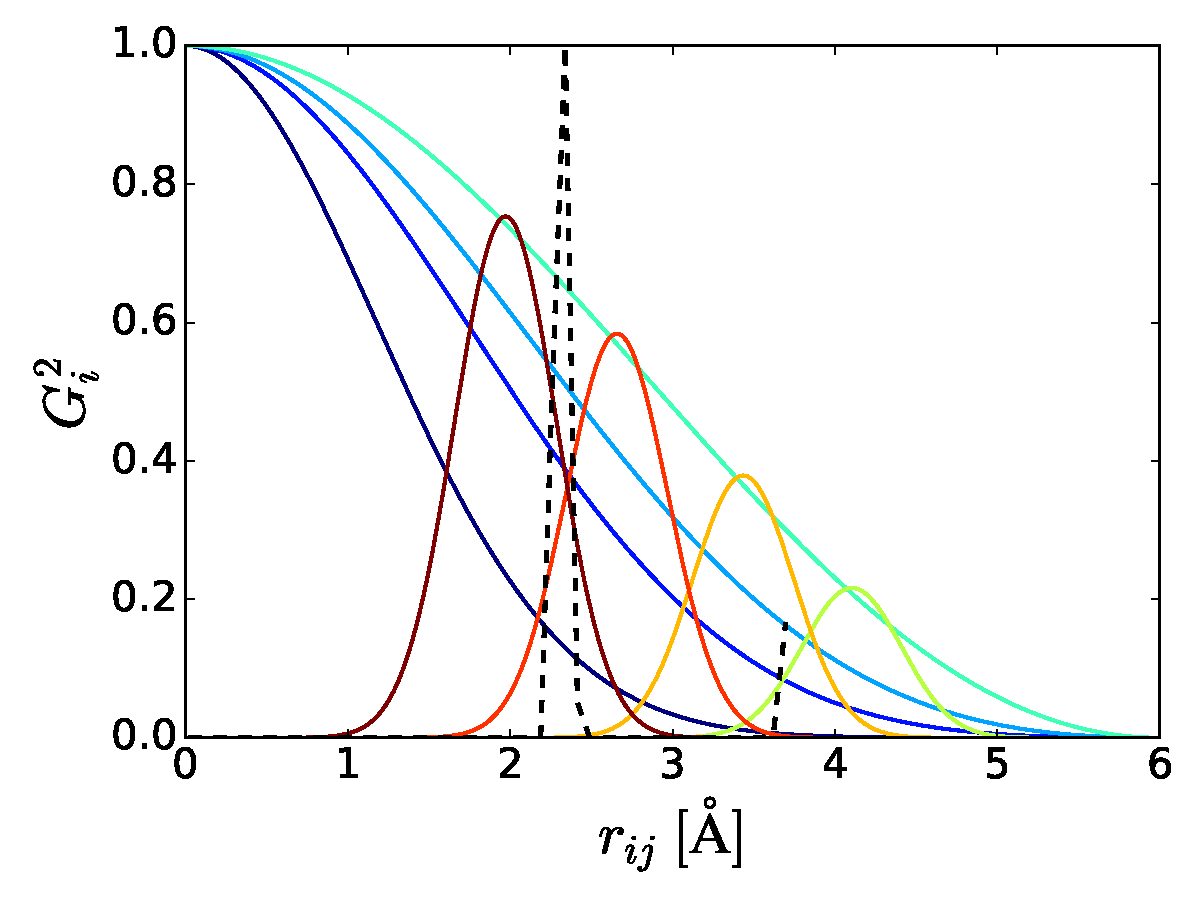
\includegraphics[width=\textwidth]{Figures/Results/SiInitialSymmG2.pdf}
 \end{minipage}
\quad
\begin{minipage}{0.48\linewidth}
 \subcaption{Angular symmetry functions}
 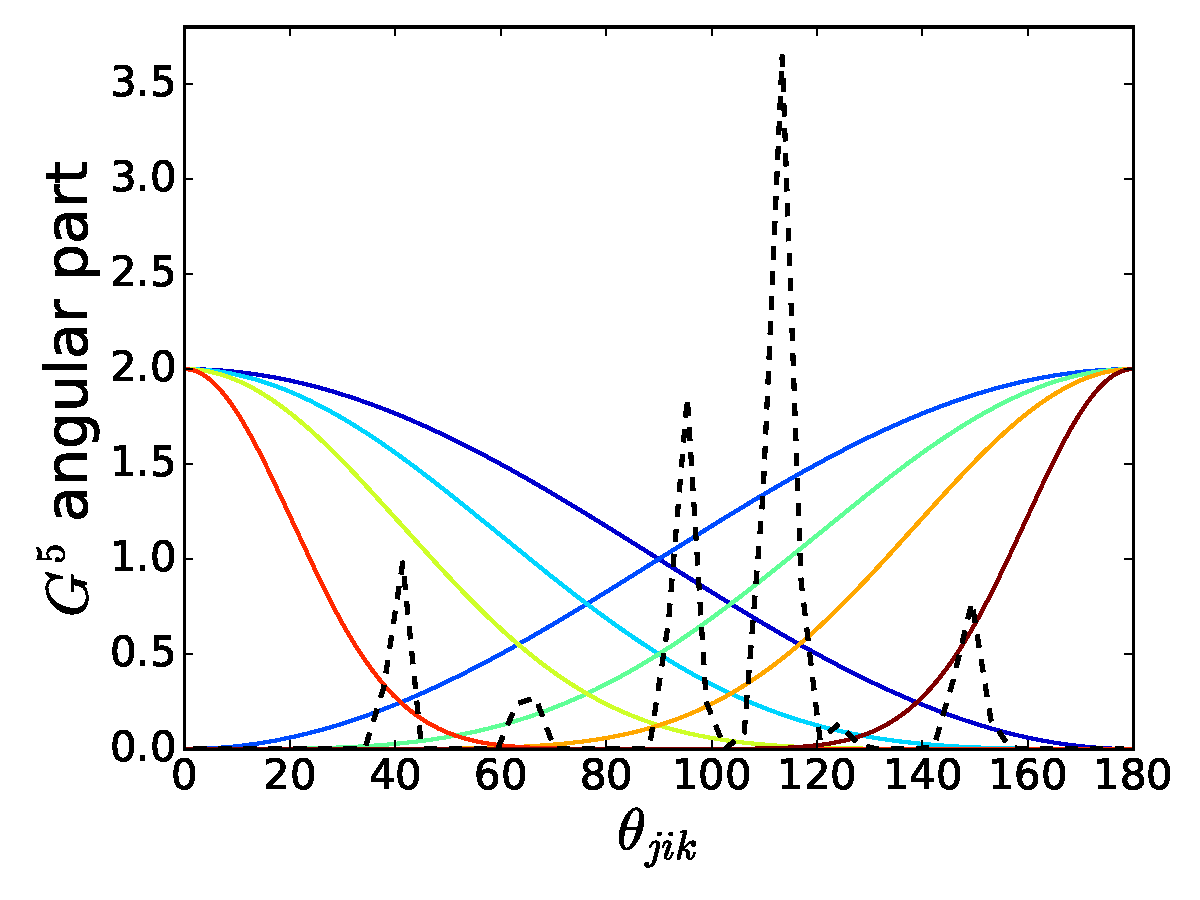
\includegraphics[width=\textwidth]{Figures/Results/SiInitialSymmG5.pdf}
\end{minipage} 
  \caption{Initial set of 8 $G_i^2$ and 16 $G_i^5$ symmetry functions for constructing a Si NNP. Only the angular part $G_i^\theta$ of 
           $G_i^5$ is displayed. Further, only 8 of these are visible because pairs of $G_i^5$ functions with identical
           angular parts overlap. 
           The dotted lines are the radial and angular distribution of neighbours defined 
           by the training set. The corresponding symmetry parameters are not included. }
  \label{fig:SiInitialSymmSet}
\end{figure}

\section{Fitting the initial data set}
According to the iterative scheme in \autoref{sec:iterativeMDsampling}, the next step in the construction process
is to create a preliminary NNP by fitting the initial data set. We do not perform a systematic search for 
optimal hyperparmameters at this intermediate stage. We have decided to employ the sigmoid activation function 
\eqref{sigmoidActivationFunction} for the remainder of the construction process
because it is more computationally efficent compared to the hyperbolic tangent, especially 
its derivative,
\begin{equation}
 f^\prime(x) = f(x) [1 - f(x)]
\end{equation}
Also, we have not experienced any significant improvement with the use of the hyperbolic tangent over the sigmoid.
Further, we have chosen the Adam optimizer for all training sessions, as this has been proven to outperform other 
schemes \cite{Kingma14}. All the employed hyperparameters are listed in \autoref{tab:hyperParamsSiInitial}. 
\begin{table} 
  \begin{center}
    \begin{tabular*}{12cm}{l @{\extracolsep{\fill}} ll}
      \toprule
      Hyperparameters &  \\ 
      \hline
      Network structure & Inputs & 24 \\
      & Outputs & 1 \\
      & Hidden layers & 1 \\
      & Hidden nodes & 10 \\
      & Activation & Sigmoid \\ 
      Training & Training set size & 3900 \\
      & Test set size & 440 \\
      & Mini-batch size & 100 \\
      & Number of epochs & 20125 \\
      & Test set RMSE tolerance & 1.0 meV \\
      & Optimizer & Adam \\
      & Initial learning rate & 0.05 \\
      & Weight initialization & $U \in [-0.1, 0.1]$ \\
      & Bias initialization & Zeros \\
      \bottomrule
      \end{tabular*} 
    \end{center}
    \captionsetup{width=12cm}
      \caption{Hyperparameters used in the fitting of the initial data set sampled from Stilling-Weber Si simulations. 
	       The data set is split into a training set and a test set, where the latter is 10 \% of the total number of 
	       structures.} 
  \label{tab:hyperParamsSiInitial} 
\end{table}
The symmetry-transformed training data has been shifted so that each symmetry function has zero-mean, and 
the minimum and maximum value of each symmetry function over the training set is stored for detecting 
extrapolating structures in the next step. 
Overfitting is detected by the following test,
\begin{minted}{Python}
if testRMSE / trainRMSE > 10:
    print 'Overfitting is occuring, training ends'
    break
\end{minted}
Several preliminary runs showed the test set RMSE to flatten out at about 1.0 meV, and we therefore decided 
to stop training if an error below this threshold was obtained, which occured after 20125 epochs. 
The final test set RMSE was 0.992 meV. 

\section{Iterative sampling} \label{sec:SiIterativeSampling}
After the initial fit, we apply the preliminary NNP in MD simulations to find new relevant structures not present 
in the current training set. The Si system is prepared in the same manner as the Stillinger-weber runs above. 
We use the minimum and maximum symmetry function values stored in the previous step to detect extrapolating
configurations according to the procedure described in \autoref{sec:iterativeMDsampling}. Each time a structure
leads to a symmetry value outside the range of the above extreme values, we sample that structure, and add 
it to the training set, 
\begin{minted}{C++}
bool extrapolation = 0;
for (int s=0; s < m_numberOfSymmFunc; s++) {
  if (symmVector[s] < m_minmax[s][0]) {
    m_minmax[s][0] = inputVector[s];
    extrapolation = 1;
  }
  else if (symmVector[s] > m_minmax[s][1]) {
    m_minmax[s][1] = inputVector[s];
    extrapolation = 1;
  }
}
\end{minted}
where \texttt{m\_minmax} is a vector containing the minimum and maximum values of each symmetry function.
After a certain number of new structures is added, the NN fit is refined by training on the extended data set. 
The NNP simulations are carried out for several temperatures $T \in [0,500] \, \mathrm{K}$. 
This iterative sampling process is continued until no new extrapolating structures are found, which occurs 
after three iterations. A total of 578 structures are added, resulting in an extended data set of 4984 training examples. 

Next, we employ the multiple-NN method (\autoref{sec:iterativeMDsampling}) to identify new structures 
that are \textit{within} the range of existing symmetry values, but located in regions of configuration space 
that are poorly represented in the training set. First, we train four NNs with different architectures on 
the complete training set to similar accuracies. 
Then, we run several MD simulations with one of these NNPs
to generate a large number configurations. The atomic coordinates are stored with the command
\begin{lstlisting}[style=lammps]
dump configs all custom 1 configs.txt id x y z vx vy vz
\end{lstlisting}
The same hyperparameters as in \autoref{tab:hyperParamsSiInitial} are used, 
except that the RMSE tolerance is changed to 5 meV. Lastly, we run pseudo-simulations with the other three NNPs
on the configurations above, 
\begin{lstlisting}[style=lammps]
rerun configs.txt dump x y z vx vy vz
compute peAtom all pe/atom
dump potEnergy chosen custom 1 potEnergy.txt id c_peAtom
\end{lstlisting}
and compare the predicted potential energies of the atoms in group \texttt{chosen}, which are randomly selected. 
Any structures for which the energy disagreement is significant, is added to the data set. An example of a 
potential energy comparison for a single atom is shown in \autoref{fig:multipleNNP}. 
\begin{figure}
\centering
  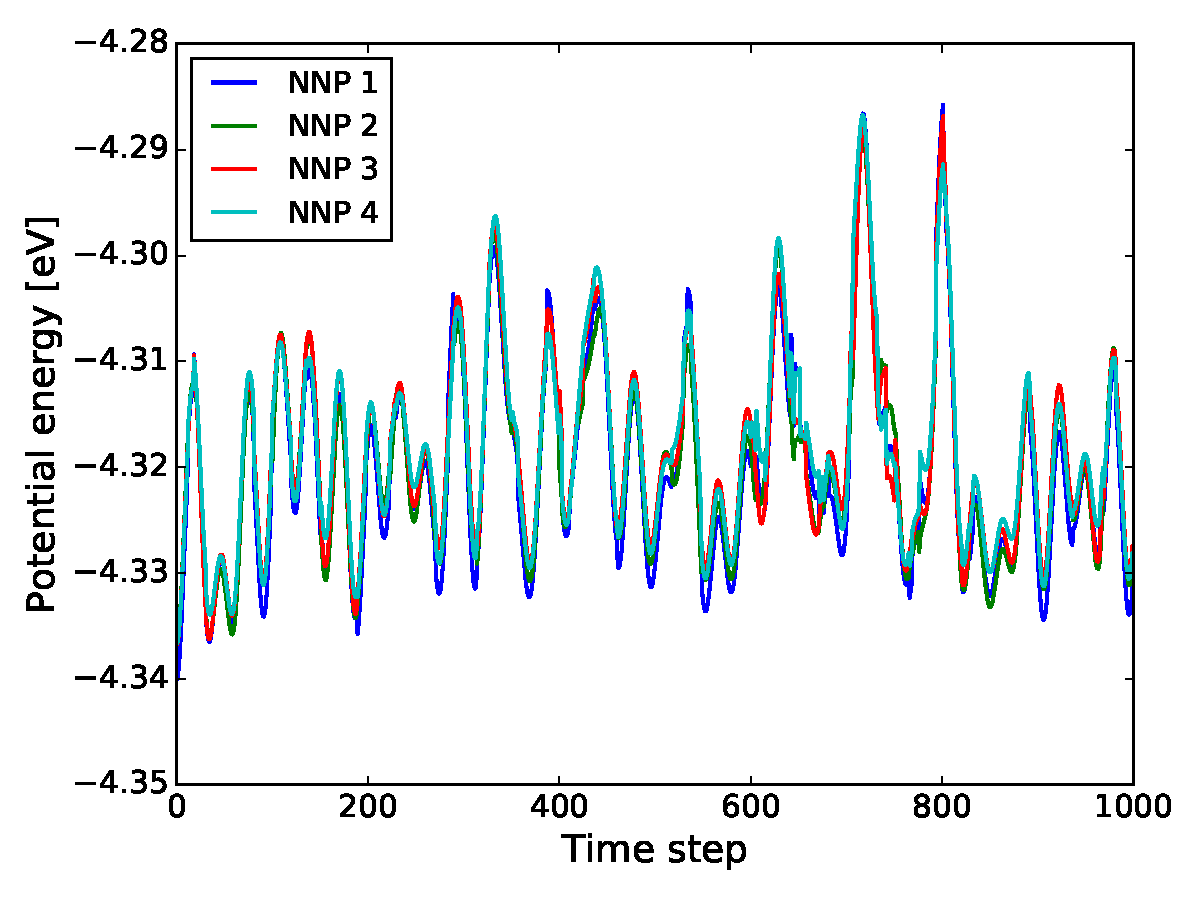
\includegraphics[width = 0.7\linewidth]{Figures/Results/multipleNNP.pdf}
  \caption{Example plot of the multiple-NN method. Four NNs with different architectures have been fitted to the same 
           data set to similar accuracies. Then, several configurations are generated with one of these NNPs, and 
           the potential energy predictions of each NNP for these structures are compared. The plot shows 
           the energies of a single atom.}
  \label{fig:multipleNNP}
\end{figure}
The simulations are carried out at an initial temperature of $T = 300$ K, and the first 1000 time steps 
of one of these simulations are displayed. For each structure, we measure
\begin{equation}
 \Delta E = E_{\max} - E_{\min}
\end{equation}
where $\Delta E$ is the difference between the maximum $E_{\max}$ and minimum $E_{\min}$ energy prediction
of the four NNPs on that structure. Any configuration for which, 
\begin{equation}
 \Delta E > \epsilon
\end{equation}
is added to the training set, where $\epsilon$ is a constant of choice. We have found that setting 
$\epsilon$ equal to the RMSE tolerance, $\epsilon=5$ meV, is an adequate choice. 

After adding 1595 new structures with the multiple-NN scheme, resulting in a final data set of 6579 training examples,
we consider the sampling as complete.



\section{Fitting the final data set}
Now that the iterative sampling scheme is finished, we are ready to construct the final NNP. 
To investigate if the symmetry function set needs to be adjusted, we calculate the range of each symmetry function 
on the training data. We find that the $G_i^5$ functions with a cutoff of $R_c = \SI{3.0}{\angstrom}$ have a very small range 
of values, thus we change the cutoff to $R_c = 4.0$. Other than that, no adjustments are made. 

To find the optimal NN architecture, we perform a grid search of different 
number of hidden layers $L$ and nodes in each hidden layer $n_l$. 
For each architecture $(L,n_l)$ we perform a training session of 40000 epochs, and for every session we store 
the smallest RMSE obtained, together with the number of epochs and the time elapsed to reach this RMSE. 
We use the same hyperparamaters as in \autoref{tab:hyperParamsSiInitial} (with various architectures), 
except that no RMSE tolerance is set, and the mini-batch size is changed to 200 to decrease the error oscillations. 
We assume that no more than two layers are needed to fit the Si potential, and the maximum number of nodes has been 
set to 32.
\begin{table} 
\centering
    \begin{tabular*}{10cm}{l @{\extracolsep{\fill}} llll}
      \toprule
      Layers & Nodes & RMSE & Epoch & Time \\ 
      \hline
      $L=1$ & 4  & 4.445 & 37035 & 575 \\
            & 8  & 2.250 & 37305 & 570 \\
            & 12 & 2.303 & 37980 & 622 \\
            & 16 & 2.201 & 39780 & 630 \\
            & 20 & 1.860 & 36180 & 617 \\ 
            & 24 & 1.928 & 37305 & 621 \\
            & 28 & 2.407 & 39375 & 697 \\
            & 32 & 2.214 & 38700 & 672 \\
      $L=2$ & 4  & 2.947 & 39960 & 750 \\
            & 8  & 1.933 & 36180 & 671 \\
            & 12 & 1.450 & 37350 & 766 \\
            & 16 & 1.791 & 32265 & 633 \\
            & 20 & 1.492 & 24840 & 546 \\
            & 24 & 2.118 & 37620 & 819 \\
            & 28 & 1.455 & 37350 & 895 \\
            & 32 & 2.008 & 14895 & 344 \\
      \bottomrule
      \end{tabular*} 
    \captionsetup{width=12cm}
      \caption{Results of a grid search for finding the optimal NN architecture to fit the final Si training set. 
               Each NN architecture is trained for 40000 epochs, and the smallest RMSE obtained during each session
               are listed, together with the number of epochs and time elapsed to reach this RMSE. 
               The RMSEs are in units of meV, while the time is measured in seconds.} 
  \label{tab:gridSearch} 
\end{table}

The results are listed in \autoref{tab:gridSearch}. We immidiately observe that all RMSEs lie in a range of about 1.5-2.5 meV, except for the two cases where $n_l = 4$. 
This tells us that the quality of the fit is not very sensitive to the NN size. Some of the two-layer NNs
converge at an earlier epoch, but they do not produce significantly better fits, and since each epoch 
takes a longer time, they do not necessarily converge more \textit{quickly}. Ideally, we should have trained each 
NN several times and calculated averages, but the above analysis is sufficient to conclude that the choice of NN size 
is not important to the quality of the fit. For computational efficiency of the eventual NNP,
we therefore decide to continue using 1 layer and 10 nodes.
\begin{table} 
\centering
    \begin{tabular*}{12cm}{l @{\extracolsep{\fill}} ll}
      \toprule
      Hyperparameters &  \\ 
      \hline
      Network structure & Inputs & 24 \\
      & Outputs & 1 \\
      & Hidden layers & 1 \\
      & Hidden nodes & 10 \\
      & Activation & Sigmoid \\ 
      Training & Training set size & 5922 \\
      & Test set size & 657 \\
      & Number of epochs & 11000 \\
      & Optimizer & Adam \\
      & Initial learning rate & 0.05 \\
      & Weight initialization & $U \in [-0.1, 0.1]$ \\
      & Bias initialization & Zeros \\
      \bottomrule
      \end{tabular*} 
    \captionsetup{width=12cm}
      \caption{Hyperparameters used in the fitting of the final training set for construction of the Si potential.} 
  \label{tab:hyperParamsSiFinal} 
\end{table}

The hyperparameters of the final NN fit are listed in \autoref{tab:hyperParamsSiFinal}. As for the initial fit, 
the training data is shifted so that each symmetry function has zero-mean. This, in combination with zero-centered 
(small) weights and biases, prevent pre-mature saturation of the sigmoid activation function, which is of great importance 
for the quality of the fit.

To investigate whether offline or online learning produce the best fit, we run several training sessions employing both. 
We find that offline learning consequently results in smaller RMSEs, thus we decide to use this method for the final fit. 
This is slower than online learning, but since we work with quite small data sets, convergence speed is not an issue, 
as we can see from \autoref{tab:gridSearch}. 

The NN is trained for 40000 epochs, and for every 1000 epochs the current NN parameters 
and RMSE are stored. When training is finished, the NN with the smallest RMSE is selected as the final NNP. 
The best fit was obtained after 11000 epochs, with an RMSE of 0.864 meV. This result is similar to other studies
employing the Behler-Parrinello method for NN interpolation \cite{Behler07,Artrith12,Natarajan16} .  

We have only fitted energies, and not forces, thus the exact force RMSE is not easily available. This would have required 
the computation of Stillinger-Weber forces for all configurations sampled from NNP simulations, and vice versa.
However, a good estimate can be obtained by running a SW simulation to generate a large number of configurations, and 
store the total force on a single atom at each time step. Then, we run a pseudo-simulation with the NNP on these configurations, 
and compare the computed forces on the same atom. The resulting force RMSE is 41.2 meV, 
which is also similar to other studies \cite{Artrith12,Natarajan16}. 
As for the Lennard-Jones NNP (\autoref{sec:LJValidation}), the RMSE of the forces is between 1-2 orders of magnitude 
larger than that for the energy.
\begin{figure}
\centering
  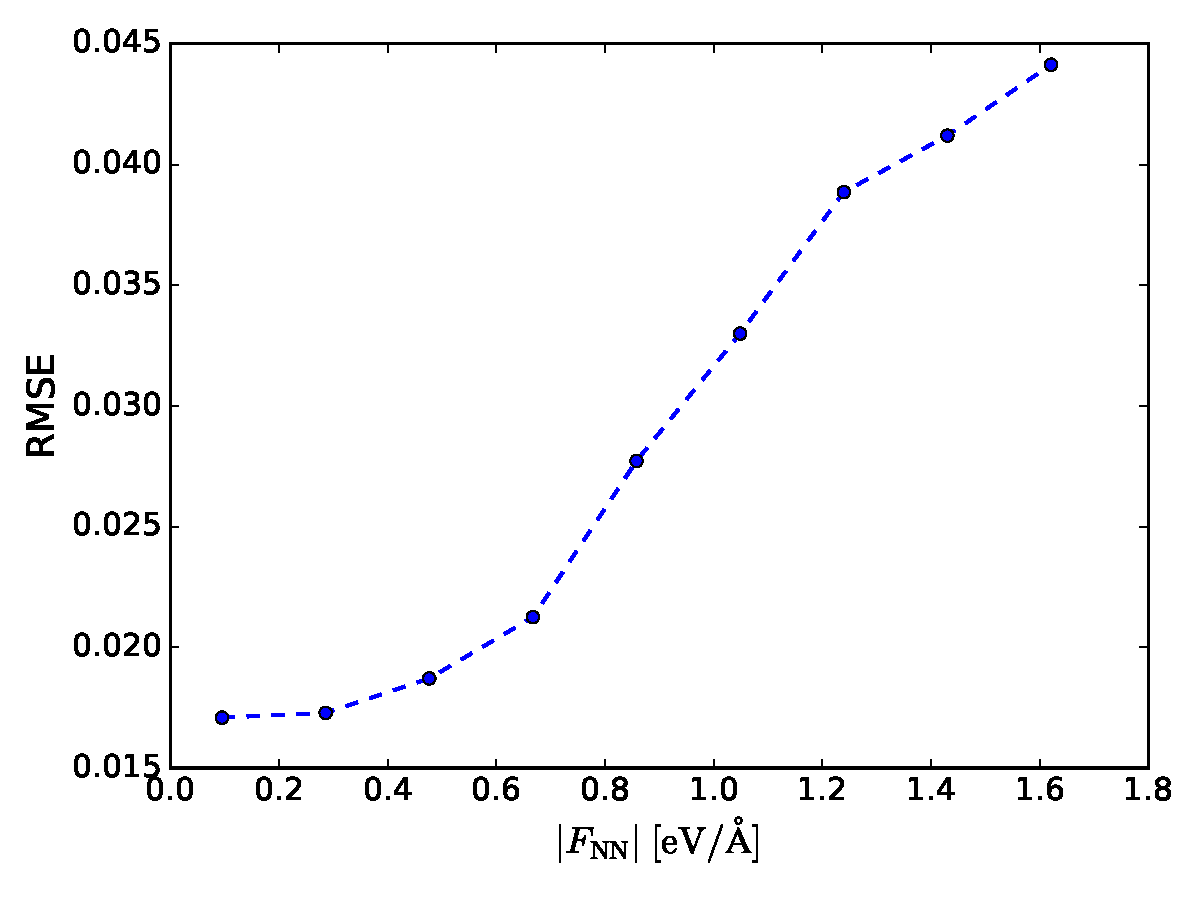
\includegraphics[width = 0.7\linewidth]{Figures/Results/SiForces.pdf}
  \caption{The RMSE of the Si NNP force predictions on a single atom as a function of the total force on the atom,
	   demonstrating a clear correlation. 
	   The force errors were calculated based on 3000 configurations generated by Stillinger-Weber simulations.}
  \label{fig:SiForces}
\end{figure}

We also wish to investigate if there is any correlation between the force error and the magnitude of the force. 
This can be done by binning the set of force errors calculated above, and computing the RMSE of each bin, shown 
in \autoref{fig:SiForces}. The data points are placed at the bin centers. We clearly see that there 
is a correlation, and that the error of the strongest forces are significantly larger than for small forces. 
This tells us that the large potential gradient-regions of configuration space do not have a sufficiently
high density in the training set, despite the use of the sampling algorithm \eqref{samplingAlgorithmModified}
for the initial data set. 



\section{Applying the NNP}
Calculating fitting errors is not sufficient for assessing the applicability of a NNP. 
To properly validate the potential we have constructed, we need to evaluate its accuracy in MD simulations.
For validation, we have chosen to confirm that the crystal structure of Si and various mechanical properties are reproduced by the NNP
by comparing with Stillinger-Weber results. 
\begin{figure}
\centering
  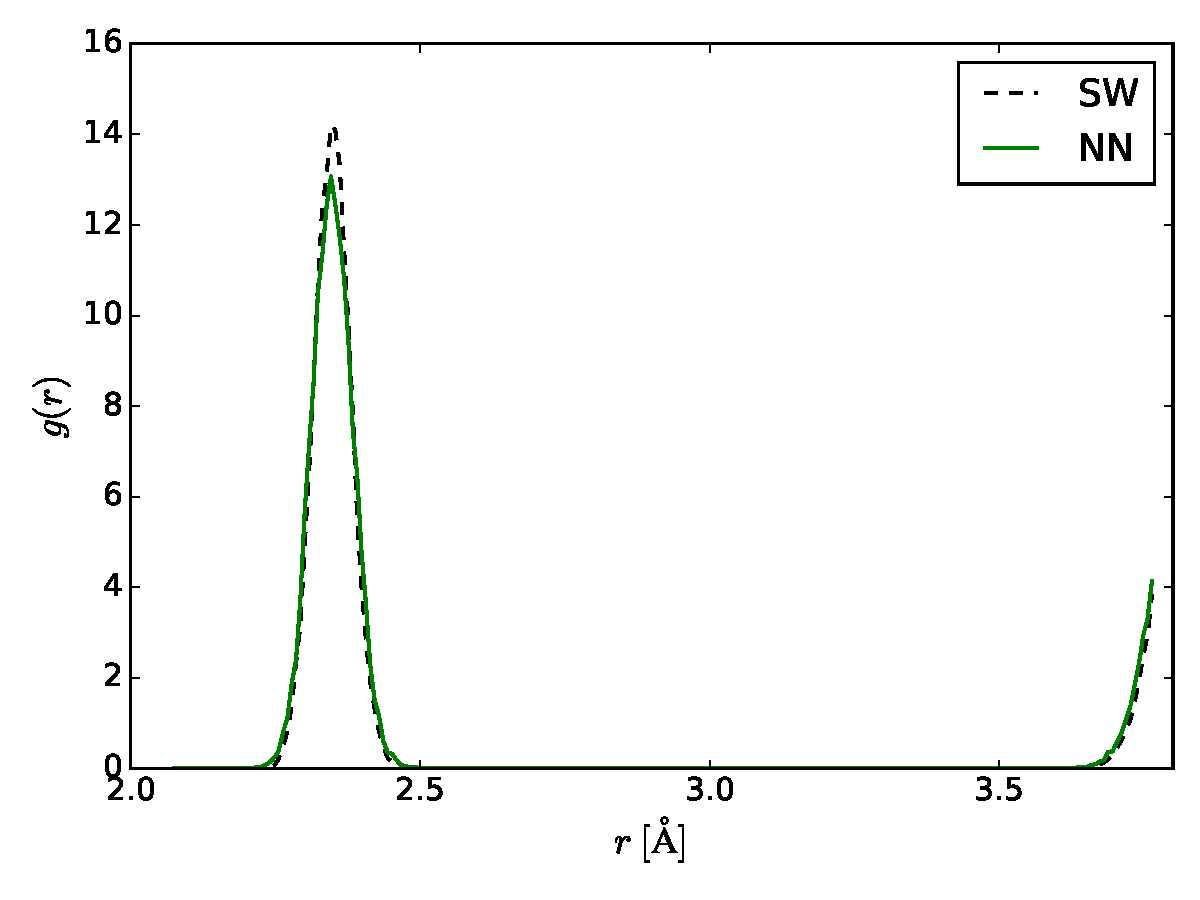
\includegraphics[width = 0.8\linewidth]{Figures/Results/radialDist.pdf}
  \caption{Comparison of the radial distribution function of a Stillinger-Weber (SW) simulation and 
           a NNP simulation of a Si crystal at temperature of $T \approx 150$ K. The crystal structure 
           of Si is reproduced by the NNP, with a small difference attributed to the increased kinetic 
           energy of the atoms due to the energy error. }
  \label{fig:radialDist}
\end{figure}

\subsection{Radial distribution function}
The radial distribution function $g(r)$, (or pair correlation function) of an atomic system is a measure of how 
particle density varies as a function of distance from a reference atom. If a system is randomly distributed, all distances
are equally probable, and $g(r)$ is unity for all distances. Any devations from unity signifies an ordered structure.
The typical shape of $g(r)$ for a crystal lattice is a flat region for small distances due to repulsive forces, 
followed by a series of peaks corresponding to bond lengths. 

To measure $g(r)$, we preare a system consisting of 1000 Si atoms on a diamond cubic lattice with a lattice constant 
of $b = \SI{5.431}{\angstrom}$. The simulation box is cubic with sides $5L$, where $L$ is the length of one unit cube.
The initial temperature is $T = 300$ K, and NVE-integration is performed, creating a system trajectory consistent with 
the microcanonical ensemble. The system is equilibrated for 10 ps, with a time step of $\Delta t = 0.001$ ps. Then, 
$g(r)$ is calculated every 100 time steps for 1000 time steps, and an average of these 10 measurements are obtained. 

The above simulation is executed with both the NNP and the SW potential. The resulting distributions are 
depicted in \autoref{fig:radialDist} for $r \in [2.0, r_c]$, with a cutoff of $r_c = 3.77118$ as above. 
We observe that the distinct crystal structure of Si is reproduced, but the peak centered at $r \approx \SI{2.3}{\angstrom}$
is slightly wider and less tall than than that for SW. This difference is attributed to the error of the energy fit, 
which leads to a slight increase in the kinetic energy of the atoms, resulting in larger vibrations. 

\subsection{Mechanical properties}
To further validate the NNP, we measure the bulk modulus, the shear modulus and the Poisson ratio of the Si crystal in 
NNP simulations. Bulk modulus $K$ is the coefficient that relates stress to strain under uniform compression,
\begin{equation}
 \frac{F}{A} = K\frac{\Delta V}{V_0}
\end{equation}
where $F/A$ is the uniform pressure (stress), and $\Delta V/V_0$ is the induced relative volume change (strain). 
A material with a large bulk modulus experiences a small volume change when pressure is applied. Note that the material 
only changes volume, not shape, under a uniform compression.

A force that is applied tangentially (or transversely) to one face of an object is called a \textit{shear} stress. 
Shear stress changes the shape of an object, but not volume. 
Shear modulus $G$ is the coefficient that relates shear stress to shear strain.
\begin{equation}
 \frac{F}{A} = G\frac{\Delta x}{y}
\end{equation}
where $\Delta x/y$ is the shear strain. 

When a material experiences a compressive force, it tends to expand in directions perpendicular to the direction of compression. 
Conversely, if the material is stretched, it tends to \textit{contract} in the perpendicular direction. The Poisson 
ratio $\nu$ is the ratio of relative contraction to relative expansion, or vice versa. More generally, it is the ratio 
of transverse strain $\epsilon_\mathrm{trans}$ to longitudinal strain $\epsilon_\mathrm{long}$,
\begin{equation}
 \nu = -\frac{\epsilon_{\mathrm{trans}}}{\epsilon_\mathrm{long}}
\end{equation}
These quantities can be obtained by employing Hooke's law. For an anisotropic material like Si, this is written as a tensor 
equation
\begin{equation}
 \sigma_{ij} = c_{ijkl}\epsilon_{kl}
\end{equation}
where $c_{ijkl}$ is a fourth rank \textit{stiffness} tensor relating stress $\sigma_{ij}$ and strain $\epsilon_{kl}$. 
However, the cubic symmetry of Si allows us to specify the stiffness tensor as a matrix (tensor of rank two)
with only three independent components $c_{11}$, $c_{12}$ and $c_{44}$, called \textit{elastic constants}. 
The bulk modulus, shear modulus and Poisson ratio 
is then calculated by the below formulas \cite{Hopcroft10}. 

\noindent Bulk modulus:
\begin{equation}
 B = \frac{c_{11} + 2c_{12}}{3}
\end{equation}
Shear modulus: 
\begin{equation}
 S = c_{44}
\end{equation}
Poisson ratio:
\begin{equation}
 \frac{1}{1 + \frac{c_{11}}{c_{22}}}
\end{equation}
To measure $c_{11}$, $c_{12}$ and $c_{44}$ in a simulation, we employ a set of example scripts contained in the LAMMPS distribution%
\footnote{\href{https://github.com/johnands/lammps/tree/master/examples/ELASTIC}
{https://github.com/johnands/lammps/tree/master/examples/ELASTIC}}.
These are slightly modified so that our NNP is employed to compute energies and forces instead of SW. 
The elastic constants are obtained by deforming the simulation box and calculating the induced stress. 
\begin{table}[h] 
\centering
    \begin{tabular*}{12cm}{l @{\extracolsep{\fill}} lll}
      \toprule
      & NNP & Analytic SW \cite{Cowley88} & Relative error  \\ 
      \hline
      Bulk modulus    & 103.0  & 101.4 &  1.58 \% \\
      Shear modulus   & 53.6   & 56.4  &  5.22 \% \\
      Poisson ratio   & 0.348  & 0.335 &  3.88 \% \\
      \bottomrule
      \end{tabular*} 
    \captionsetup{width=12cm}
      \caption{Various mechanical properties measured from NNP simulations of Si. The analytical values 
	       for Stillinger-Weber are included, along with the relative error. The bulk modulus and 
	       shear modulus have units of GPa, while the Poisson ratio is unitless.} 
  \label{tab:SiMechanical} 
\end{table}

The results are listed in \autoref{tab:SiMechanical}. We observe that the SW values are reproduced with small relative errors, 
demonstrating that also the mechanical properties of the Si crystal are modelled correctly with the NNP.
Since SW has been used to compute reference energies for the NNP fit, we do not compare with experimental values, as 
this would only assess the accuracy of SW, not the NNP. 







\part{Conclusions and future work}

\chapter{Summary and conclusion}
In this thesis, we developed a method for constructing high-dimensional neural network potentials. This method was applied
for the construction of an inter-atomic potential for solid-state Si, and the radial distribution function,
bulk modulus, shear modulus and Poisson ratio were measured for benchmarking.

To find atomic structures that were relevant for the intended application of the potential, 
we implemented a custom \texttt{compute} in LAMMPS 
that sampled atom-centered configurations and total potential energies according to a modified sampling algorithm. 
This \texttt{compute} was used to sample configurations from Stillinger-Weber simulations, which constituted the initial 
training data for the construction of the Si potential. 

We implemented the Behler-Parrinello method to deal with the fixed dimensionality and symmetry problems of neural networks. 
A set of symmetry functions was created for the initial Si training data. This set was compared with 
the radial and angular distribution of atoms in the training data to evaluate its ability to adequately probe 
the atomic environments. The symmetry functions were also used in an iterative sampling scheme to find new relevant structures 
outside the range of existing symmetry values. Further, the multiple-NN method was employed to detect
regions of configurations space poorly represented in the training set. 

We developed a set of Python scripts to train neural networks to fit the sampled data sets. 
The machine learning library TensorFlow was used for this purpose. Various properties of the fitting procedure were 
investigated by training a one-dimensional neural network to reproduce the truncated and shifted Lennard-Jones potential.
We found that the NN were able to accurately fit the functional form of the LJ potential, and obtained a RMSE 
of 0.896 meV. The absolute error was plotted as a function of inter-atomic distance, demonstrating that the error 
was largest for small distances. 

Further, TensorFlow was used in combination with the BP method to construct a potential for Si by 
fitting data sets sampled from both Stillinger-Weber and preliminary NNP simulations. The fit was gradually refined 
with the iterative sampling scheme mentioned above. A final RMSE of 0.864 meV was obtained, 
which was comparable with other studies. 

Lastly, we applied the eventual Si NNP in MD simuations to evaluate its accuracy. 
The radial distribution function was measured, and was found to be in good agreement with Stillinger-Weber. 
The small deviations were attributed to an increase in the kinetic energy of the atoms due to the fitting error.
Further, various mechanical properties of the NNP Si system were calculated, specifically the bulk modulus, the shear 
modulus, and the Poisson ratio. The results had relative errors in the range 1.5-5.2 \% when compared to the analytic 
Stillinger-Weber values. 


\subsubsection{Properties of a high-dimensional neural network potential} 
When developing a new PES, it is useful to define a set of properties that the ''ideal'' potential 
should possess. These may serve as guiding principles during the construction process, and is also a good 
starting point for comparing different types of potentials. Behler \cite{Behler11general} lists 10 requirements
that the ideal potential should meet. We will now evaluate our NNP in light of these requirements. 
\begin{enumerate}
 \item \textit{The potential should be accurate, i.e.\ produce results that are in good agreement with experiments. 
       Ideally, it should be constructed using \textit{ab inito} methods.} 
       
       The NNP can be fitted to \textit{ab inito} data to arbitrary accuracy, and 
       can therefore be considered an \textit{ab inito} potential.  
 \item \textit{There should be ways to systematically detect situations where the potential is not suffientently accurate, 
       and improve it without too much effort.} 
       
       The NNP can be systematically improved by employing the iterative scheme proposed in \autoref{sec:selectingTrainingData}.
 \item \textit{The potential should be unbiased and applicable to all types of systems and chemical bonding.} 
       
       The NNP has no pre-defined functional form, and its applications are unlimited as 
       long as the production of \textit{ab inito} reference energies is feasible. However, for systems containing 
       several different chemical elements, the symmetry function vectors grow very large, and the symmetry function sets 
       get increasingly difficult to set up.
 \item \textit{The potential should enable the breaking and making of bonds.}
       
       The NNP is able to model the breaking and making of bonds as long as the reference set contains
       configurations that are relevant for these processes.  
 \item \textit{The potential should be high-dimensional, i.e.\ depend on all degress of freedom of the system.}
       
       The NNP is high-dimensional because it depends on all the degrees of freedom of the chemical environment of each atom. 
 \item \textit{The construction of the potential should be as automated as possible.} 
       
       The NN parameters, and hence the functional form of the NNP, is automatically optimized. However, 
       the determination of symmetry parameters and other hyperparmameters is to a certain degree empirical. 
       Further, training data can be automatically produced by MD simulations, but the physical conditions 
       of each simulation and the sampling of configurations must be carefully considered. 
 \item \textit{The potential should be predictive, i.e.\ be reliable for atomic configurations that have not been used in the 
       construction.}
       
       The NNP is generally not able to extrapolate, and is thus reliable only for configurations that are within 
       the configuration space spanned by the training set.
       
 \item \textit{The potential should be fast to evaluate.}
 
       The NNP is several orders of magnitude faster to evalute than e.g.\ DFT or Hartree-Fock potentials, 
       and thus enables MD simulations with \textit{ab inito} accuracy on larger scales of space and time.  
       It is however notably slower compared to empirical potentials like Lennard-Jones or Stillinger-Weber. 
 \item \textit{The construction of the potential should not require much computation time.}
 
       Training does not require much computation time, but calculating reference energies for thousands of configurations
       is time consuming. 
 \item \textit{To compute forces, analytic derivatives of the potential should be available.}
       Analytic derivatives of both the NN and the symmetry functions are readily available. 
\end{enumerate}
We observe that our NNP fulfills the majority of the 10 requirements stated above.  
None of the potentials currently available, including NNPs, are ideal. 
However, NNPs are an excellent tool for multi-scale physics. They connect the realms of quantum mechanics 
and molecular dynamics by enabling \textit{ab inito} simulations on a larger scale of space and time than what is feasible 
for convential \textit{ab inito} MD. This property, in addition to the unbiased and transferable nature of the 
Behler-Parrinello approach, 
signifiy that research in this field will be increasingly important in the future. 

\chapter{Prospects and future work}
An important aspect of the construction of NNPs is to employ a suitable \textit{ab inito} method to calculate reference energies.
In this thesis, we have computed target energies with common empirical potentials, and thus not constructed \textit{ab inito}
potentials. The most obvious extension to the current work is therefore to employ methods like Hartree-Fock or Density Functional theory 
to obtain energies. However, there is also much room for improvement in other areas. 

\section{Force accuracy}
We saw in chapters \autoref{sec:LJValidation} and \autoref{sec:SiPotentialResults} that the force RMSE is generally 
1-2 orders of magnitude larger than that for the energy. The forces determine the dynamics of a simulation, and their accuracy 
is therefore of vital importance. One way to improve the force RMSE is to employ the modified cost function
\eqref{CFDA} to fit both energies and forces. To do this, we must compute reference forces in addition to energies, 
which is obviously more computationally demanding. However, according to Behler \cite{Behler15}, adding forces to the training 
data reduces the required number of reference energies, leading to a smaller data set. 

Further, we have repeatedly observed that the fitting error increases for large forces and energies, which can be avoided 
by including more high-gradient configurations in the training data. We employed a sampling algorithm
\eqref{samplingAlgorithmModified} for this purpose, and although this reduced the problem, it did not remove it entirely. 
Improved sampling algorithms could therefore be an improvement to this work. 

\section{Other systems}
We have constructed a NNP for a system consisting of only one chemical element, but the Behler-Parrinello (BP) method 
is applicable to systems containing several elements. The BP scheme is high-dimensional, which 
makes it suitable for studying complex systems where many degrees of freedom must be included to provide an accurate description 
of the dynamics. The BP method can also be extended to include electrostatic contributions \cite{Behler15}, 
and water $\mathrm{H_2O}$ is therefore an interesting candidate. 

NNPs are also able to model the breaking and making of bonds; studying chemical reaction dynamics is 
therefore a possibility. 

\section{Optimization}
For NNPs to serve as a multi-scale physics tool, they must be much more computationally efficient than 
\textit{ab inito} methods. Ideally, their computational efficiency should be comparable to that of empirical potentials. 
We have not performed any proper performance analysis in this thesis, but 
based on several simulations with the Si NNP, we have found that Stillinger-Weber is between 1-2 orders of magnitude faster.
Consequentially, the NNP is several orders of magnitude faster than \textit{ab inito} methods%
\footnote{\href{http://lammps.sandia.gov/bench.html}{lammps.sandia.gov/bench.html}}. 

However, optimizing the evaluations of the symmetry functions and the network may contribute to a significant speed-up. 
We have employed Armadillo to evaluate and differentiate NNPs, which may not the most efficient approach. Further, 
the size of the NN and the symmetry function set may be reduced by performing a more thorough hyperparmeter optimization. 














\begin{appendices}

\chapter{Symmetry function derivatives} \label{app:appendixA1}
According to \eqref{forceAtomkChainRule}, we need the derivatives of the symmetry functions defined in 
\autoref{sec:symmetryFunctions} to obtain forces during simulations. Analytic derivatives have been obtained 
with SymPy, shown here for $G_i^5$,
\begin{minted}{Python}
from sympy.utilities.codegen import codegen
from sympy import *

# variables
xj, yj, zj, xk, yk, zk =  symbols('xj yj zj xk yk zk')

# parameters
eta, Rc, zeta, Lambda = symbols('eta Rc zeta Lambda')

# substitution parameters
Rj, Rk, Rj2, Rk2, RjDotRk, CosTheta, Fcj, Fck, dFcj, dFck = \
    symbols('Rj Rk Rj2 Rk2 RjDotRk CosTheta Fcj Fck dFcj dFck')

rj = sqrt(xj**2 + yj**2 + zj**2)
rk = sqrt(xk**2 + yk**2 + zk**2)
fcj = 0.5*cos(pi*rj/Rc) + 0.5
fck = 0.5*cos(pi*rk/Rc) + 0.5
rjDotrk = (xj*xk + yj*yk + zj*zk)
cosTheta = rjDotrk / (rj*rk)

F1 = 2**(1-zeta) * (1 + Lambda*cosTheta)**zeta
F2 = exp(-eta*(rj**2 + rk**2))
F3 = fcj*fck
G5 = F1*F2*F3

dG5dxj = diff(G5, xj)
dG5dxj = dG5dxj.subs(xj**2 + yj**2 + zj**2, Rj2)
dG5dxj = dG5dxj.subs(xk**2 + yk**2 + zk**2, Rk2)
dG5dxj = dG5dxj.subs(sqrt(Rj2), Rj)
dG5dxj = dG5dxj.subs(sqrt(Rk2), Rk)
dG5dxj = dG5dxj.subs(xj*xk + yj*yk + zj*zk, RjDotRk)
dG5dxj = dG5dxj.subs(RjDotRk/(Rj*Rk), CosTheta)
dG5dxj = dG5dxj.subs(0.5*cos(pi*Rj/Rc) + 0.5, Fcj)
dG5dxj = dG5dxj.subs(0.5*cos(pi*Rk/Rc) + 0.5, Fck)
dG5dxj = dG5dxj.subs(sin(pi*Rj/Rc)/(Rc), -2*dFcj/pi)

dG5dxk = diff(G5, xk)
dG5dxk = dG5dxk.subs(xj**2 + yj**2 + zj**2, Rj2)
dG5dxk = dG5dxk.subs(xk**2 + yk**2 + zk**2, Rk2)
dG5dxk = dG5dxk.subs(sqrt(Rj2), Rj)
dG5dxk = dG5dxk.subs(sqrt(Rk2), Rk)
dG5dxk = dG5dxk.subs(xj*xk + yj*yk + zj*zk, RjDotRk)
dG5dxk = dG5dxk.subs(RjDotRk/(Rj*Rk), CosTheta)
dG5dxk = dG5dxk.subs(0.5*cos(pi*Rj/Rc) + 0.5, Fcj)
dG5dxk = dG5dxk.subs(0.5*cos(pi*Rk/Rc) + 0.5, Fck)
dG5dxk = dG5dxk.subs(sin(pi*Rk/Rc)/(Rc), -2*dFck/pi)

print codegen(("dG5dxj", simplify(dG5dxj)), "C", "file")[0][1]
print codegen(("dG5dxk", simplify(dG5dxk)), "C", "file")[0][1]
\end{minted}
However, calculating the derivatives by hand allows us to write the expression for the derivatives in a more compact form, 
speeding up the force computations.
Thus, we compute the derivatives of all symmetry functions except $G_i^3$ in the following. The SymPy expressions serve 
as a validation of our calculations. 

\subsubsection{Notation and symmetries}
In some cases we only show the deriviative with respect to 
$r_{ij}$. Each component $\alpha$ can be calculated by
\begin{equation}
 \frac{\partial r_{ij}}{\partial \alpha} = \frac{\alpha}{r_{ij}}
\end{equation}
The following notation applies,
\begin{equation}
 r_{ij} = \Bigr(x_{ij}^2 + y_{ij}^2 + z_{ij}^2\Bigr)^{1/2} =
 \Bigr((x_j - x_i)^2 + (y_j - y_i)^2 + (z_j - z_i)^2\Bigr)^{1/2}
\end{equation}
From \autoref{sec:symmAndForces} we have the identities,
\begin{subequations}
\begin{align}
 \frac{\partial r_{ij}}{\partial x_{ij}} &= \frac{\partial r_{ij}}{\partial x_j} \label{symmetryDerivativeApp1} \\
 \frac{\partial r_{ij}}{\partial x_{ij}} &= -\frac{\partial r_{ij}}{\partial x_i} \label{symmetryDerivativeApp2}
\end{align}
\end{subequations}

\subsubsection{Derivatives of cutoff function and radial symmetry functions}
Derivative of the cutoff function \eqref{cutoffFunction}:
\begin{equation}
 \frac{\partial f_c(r)}{\partial r} = -\frac{1}{2}\frac{\pi}{r_c} \sin\left(\frac{\pi r}{r_c}\right) = M(r)
 \label{cutOffFunctionDerivative}
\end{equation}
This expression is valid for all combinations of indicies $(i,j,k)$. The derivatives w.r.t. to individual coordinates are
\begin{equation}
 \frac{\partial f_c(r_{ij})}{\partial x_{ij}} = M(r_{ij})
 \frac{x_{ij}}{r_{ij}}
 \label{cutOffFunctionDerivative1}
\end{equation}
and 
\begin{equation}
 \frac{\partial f_c(r_{ik})}{\partial x_{ik}} = M(r_{ik})
 \frac{x_{ik}}{r_{ik}}
 \label{cutOffFunctionDerivative1}
\end{equation}
while
\begin{equation}
 \frac{\partial f_c(r_{ij})}{\partial x_{ik}} = \frac{\partial f_c(r_{ik})}{\partial x_{ij}} = 0
\end{equation}
according to \eqref{symmetryDerivativeApp1}. Also, 
\begin{equation}
 \frac{\partial f_c(r_{jk})}{\partial x_{ij}} = -M(r_{jk})
 \frac{x_{jk}}{r_{jk}}
 \label{cutOffFunctionDerivative1}
\end{equation}
and 
\begin{equation}
 \frac{\partial f_c(r_{jk})}{\partial x_{ik}} = M(r_{jk})
 \frac{x_{jk}}{r_{jk}}
 \label{cutOffFunctionDerivative1}
\end{equation}
The derivative of each term in $G_i^1$ \eqref{G1} is simply equal to \eqref{cutOffFunctionDerivative}.

\noindent Derivative of $G_i^2$ \eqref{G2}:
\begin{equation}
 \frac{\partial G_i^2}{r_{ij}} = 
 \exp(-\eta(r_{ij}-r_s)^2) \left[2\eta(r_s - r_{ij}) + \frac{\partial f_c}{\partial r_{ij}}\right]
\end{equation}

\subsubsection{Derivatives of angular symmetry functions}
$G_i^4$ \eqref{G4}:
\begin{equation}
 G_i^4 = F_1(\theta)F_2(r_{ij},r_{ik},r_{jk})F_3(r_{ij},r_{ij},r_{jk})
\end{equation}
where
\begin{align}
 F_1(\theta) &= 2^{1-\zeta}(1 + \lambda \cos\theta_{ijk})^\zeta \\
 F_2(r_{ij},r_{ik},r_{jk}) &= \exp[-\eta (r_{ij}^2 + r_{ik}^2 + r_{jk}^2)] \\
 F_3(r_{ij},r_{ij},r_{jk}) &= f_c(r_{ij}) f_c(r_{ik}) f_c (r_{jk})
\end{align}
and where
\begin{equation}
 \cos\theta = \frac{x_{ij}x_{ik} + y_{ij}y_{ik} + z_{ij}z_{ik}}{r_{ij}r_{ik}}
\end{equation}
Using the product rule:
\begin{subequations}
\begin{align}
 \frac{\partial G_i^4}{\partial x_{ij}} = &\frac{\partial F_1}{x_{ij}} F_2 F_3 + 
 F_1 \left(\frac{\partial F_2}{\partial x_{ij}}F_3 + F_2\frac{\partial F_3}{\partial x_{ij}}\right) \\
 &\frac{\partial F_1}{x_{ij}} F_2 F_3 + 
 F_1 \frac{\partial F_2}{\partial x_{ij}}F_3 + F_1F_2\frac{\partial F_3}{\partial x_{ij}}
 \label{G4Derivative}
\end{align}
\end{subequations}
We have
\begin{equation}
 \frac{\partial F_1}{\partial x_{ij}} = \frac{\partial F_1}{\partial\cos\theta}
 \frac{\partial\cos\theta}{\partial x_{ij}}
\end{equation}
where
\begin{equation}
 \frac{\partial F_1}{\partial\cos\theta} = \lambda\zeta(1 + \cos\theta)^{\zeta-1} = K
\end{equation}
and 
\begin{equation}
 \frac{\partial\cos\theta}{\partial x_{ij}} = \frac{x_{ik}}{r_{ij}r_{ik}} - 
 \frac{x_{ij}\cos\theta}{r_{ij}^2}
\end{equation}
To get the corresponding expression for $x_{ik}$, simply substitute $x_{ij} \rightarrow x_{ik}$ and 
$r_{ij} \rightarrow r_{ik}$. Further, 
\begin{equation}
\begin{aligned}
 \frac{\partial F_2}{\partial x_{ij}} &= \frac{\partial F_2}{\partial r_{ij}}\frac{\partial r_{ij}}{\partial x_{ij}}  = 
 (-2\eta r_{ij}\frac{x_{ij}}{r_{ij}} - 2\eta r_{jk}\frac{x_{jk}}{r_{jk}})\exp[-\eta (r_{ij}^2 + r_{ik}^2 + r_{jk}^2)] \\
 &= -2\eta F_2 x_{ij} - 2\eta F_2 x_{jk}
\end{aligned}
\end{equation}
The corresponding expression for $x_{ik}$ is
\begin{equation}
 \frac{\partial F_2}{\partial x_{ik}} = 
 -2\eta F_2 x_{ik} + 2\eta F_2 x_{jk}
\end{equation}
Lastly, 
\begin{subequations}
\begin{align}
 \frac{\partial F_3}{\partial x_{ij}} &=  \frac{\partial f_c(r_{ij})}{\partial x_{ij}}
 f_c(r_{ik}) f_c(r_{jk}) + f_c(r_{ij})f_c(r_{ik})\frac{\partial f_c(r_{jk})}{\partial x_{ij}} \\
 &= f_c(r_{ik})\Biggr(M(r_{ij})\frac{x_{ij}}{r_{ij}}f_c(r_{jk}) - 
 f_c(r_{ij}) M(r_{jk})\frac{x_{jk}}{r_{jk}} \Biggr)
\end{align}
\end{subequations}
The corresponding expression for $x_{ik}$ is
\begin{subequations}
\begin{align}
 \frac{\partial F_3}{\partial x_{ik}} &= f_c(r_{ij})\Biggr(\frac{\partial f_c(r_{ik})}{\partial x_{ik}}f_c(r_{jk}) + 
 f_c(r_{ik}) \frac{\partial f_c(r_{jk})}{\partial x_{ik}} \Biggr) \\
 &= f_c(r_{ij})\Biggr(M(r_{ik})\frac{x_{ik}}{r_{ik}}f_c(r_{jk}) + 
 f_c(r_{ik}) M(r_{jk})\frac{x_{jk}}{r_{jk}} \Biggr)
\end{align}
\end{subequations}
Then, taking \eqref{G4Derivative} into account:
\begin{equation}
\begin{aligned}
 \frac{\partial G_i^4}{\partial x_{ij}} = &\biggr(\frac{x_{ik}}{r_{ij}r_{ik}} - \frac{x_{ij}\cos\theta}{r_{ij}^2}
 \biggr)KF_2F_3 \, - \\ &2\eta F_1F_2F_3 x_{jk} - 2\eta F_1F_2F_3 x_{ij} \, + \\
 &F_1F_2 f_c(r_{ik})\Biggr(M(r_{ij})\frac{x_{ij}}{r_{ij}}f_c(r_{jk}) +
 f_c(r_{ij}) M(r_{jk})\frac{x_{jk}}{r_{jk}} \Biggr)
\end{aligned}
\end{equation}
and for $x_{ik}$:
\begin{equation}
\begin{aligned}
 \frac{\partial G_i^4}{\partial x_{ik}} = &\biggr(\frac{x_{ij}}{r_{ij}r_{ik}} - \frac{x_{ik}\cos\theta}{r_{ik}^2}
 \biggr)KF_2F_3 \, + \\ &2\eta F_1F_2F_3 x_{jk} - 2\eta F_1F_2F_3 x_{ik} \, + \\
 &F_1F_2 f_c(r_{ij})\Biggr(M(r_{ik})\frac{x_{ik}}{r_{ik}}f_c(r_{jk}) - 
 f_c(r_{ik}) M(r_{jk})\frac{x_{jk}}{r_{jk}} \Biggr)
\end{aligned}
\end{equation}
or in terms of $x_{ij}$ and $x_{ik}$ and $x_{jk}$:
\begin{equation}
\begin{aligned}
 \frac{\partial G_i^4}{\partial x_{ij}} = &x_{ij} \biggr(-\frac{\cos\theta}{r_{ij}^2}K
 F_2F_3 - 2\eta F_1F_2F_3 \, + \\ 
 &F_1F_2M(r_{ij})f_c(r_{ik})f_c(r_{jk})\frac{1}{r_{ij}}\biggr) \, + \\
 &x_{ik}\frac{KF_2F_3}{r_{ij}r_{ik}} - x_{jk}\Bigr(F_1F_2M(r_{jk})f_c(r_{ik})f_c(r_{ij}) + 2\eta F_1F_2F_3\Bigr)\frac{1}{r_{jk}}
\end{aligned}
\end{equation}
and 
\begin{equation}
\begin{aligned}
 \frac{\partial G_i^4}{\partial x_{ik}} = &\frac{x_{ik}}{r_{ik}} \biggr(-\frac{\cos\theta}{r_{ik}^2}K
 F_2F_3 - 2\eta F_1F_2F_3 \, + \, \\
 &F_1F_2M(r_{ik})f_c(r_{ij})f_c(r_{jk})\frac{1}{r_{ik}}\biggr) + \, \\
 &x_{ij}\frac{KF_2F_3}{r_{ij}r_{ik}} + x_{jk}\Bigr(F_1F_2M(r_{jk})f_c(r_{ij})f_c(r_{ik}) - 2\eta F_1F_2F_3\Bigr)\frac{1}{r_{jk}}
\end{aligned}
\end{equation}
The derivative of $G_i^5$ \eqref{G5} is found in a similar way,
\begin{equation}
 G_i^5 = F_1(\theta)F_2(r_{ij},r_{ik})F_3(r_{ij},r_{ij})
\end{equation}
where 
\begin{align}
 F_1(\theta) &= 2^{1-\zeta}(1 + \lambda \cos\theta_{ijk})^\zeta \\
 F_2(r_{ij},r_{ik}) &= \exp[-\eta (r_{ij}^2 + r_{ik}^2)] \\
 F_3(r_{ij},r_{ij}) &= f_c(r_{ij}) f_c(r_{ik})
\end{align}
The derivative of $F_1$ is the same, while for $F_2$ we obtain
\begin{equation}
 \frac{\partial F_2}{\partial x_{ij}} = -2\eta F_2 x_{ij}
\end{equation}
and
\begin{equation}
 \frac{\partial F_2}{\partial x_{ik}} = -2\eta F_2 x_{ik}
\end{equation}
For $F_3$, 
\begin{equation}
 \frac{\partial F_3}{\partial x_{ij}} = \frac{\partial f_c(r_{ij})}{\partial x_{ij}}\frac{x_{ij}}{r_{ij}}
 f_c(r_{ik}) = M(r_{ij})f_c(r_{ik})\frac{x_{ij}}{r_{ij}}
\end{equation}
and
\begin{equation}
  \frac{\partial F_3}{\partial x_{ik}} = f_c(r_{ij})
 \frac{\partial f_c(r_{ik})}{\partial x_{ij}}\frac{x_{ik}}{r_{ik}} = 
 f_c(r_{ij})M(r_{ik})\frac{x_{ik}}{r_{ik}}
\end{equation}
so that
\begin{equation}
\begin{aligned}
 \frac{\partial G_i^5}{\partial x_{ij}} = &\biggr(\frac{x_{ik}}{r_{ij}r_{ik}} - \frac{x_{ij}\cos\theta}{r_{ij}^2}
 \biggr)KF_2F_3 -
 2\eta F_1 F_2F_3 x_{ij} \, + \\
 &F_1F_2 M(r_{ij})f_c(r_{ik})\frac{x_{ij}}{r_{ij}}
\end{aligned}
\end{equation}
and 
\begin{equation}
\begin{aligned}
 \frac{\partial G_i^5}{\partial x_{ik}} = &\biggr(\frac{x_{ij}}{r_{ij}r_{ik}} - \frac{x_{ij}\cos\theta}{r_{ik}^2}
 \biggr)KF_2F_3 -
 2\eta F_1 F_2F_3 x_{ik} \, + \\
 &F_1F_2 M(r_{ik})f_c(r_{ij})\frac{x_{ik}}{r_{ik}}
\end{aligned}
\end{equation}
In terms of $x_{ij}$ and $x_{ik}$:
\begin{equation}
\begin{aligned}
 \frac{\partial G_i^5}{\partial x_{ij}} = \, &x_{ij} \biggr(-\frac{\cos\theta}{r_{ij}^2}K
 F_2F_3 - 2\eta F_1F_2F_3 + \\ &F_1F_2M(r_{ij})f_c(r_{ik})\frac{1}{r_{ij}} \biggr) \, + 
 x_{ik}\frac{KF_2F_3}{r_{ij}r_{ik}}
\end{aligned}
\end{equation}
and 
\begin{equation}
\begin{aligned}
 \frac{\partial G_i^5}{\partial x_{ik}} = \, &x_{ik} \biggr(-\frac{\cos\theta}{r_{ik}^2}K
 F_2F_3 - 2\eta F_1F_2F_3 + \\ &F_1F_2M(r_{ik})f_c(r_{ij})\frac{1}{r_{ik}} \biggr) \, + 
 x_{ij}\frac{KF_2F_3}{r_{ij}r_{ik}}
\end{aligned}
\end{equation}


\chapter{Symmetry function parameters} \label{app:symmFuncParameters}
Here we list the symmetry parameters employed in the construction of the Si NNP in \autoref{sec:SiPotentialResults}.
\begin{table}[h] 
  \begin{center}
    \begin{tabular*}{6cm}{l @{\extracolsep{\fill}} ll}
      \toprule
      $r_c$ & $\eta$ & $r_s$ \\ 
      \hline
      6.0 & 0.3 & 0 \\
      6.0 & 0.1 & 0 \\
      6.0 & 0.05 & 0 \\
      6.0 & 0.005 & 0 \\
      6.0 & 5.0 & 4.2 \\ 
      6.0 & 5.0 & 3.5 \\
      6.0 & 5.0 & 2.7 \\ 
      6.0 & 5.0 & 2.0 \\
      \bottomrule
      \end{tabular*} 
    \end{center}
    \captionsetup{width=12cm}
      \caption{Symmetry function parameters for $G_i^2$ employed in the fitting of the Si NNP in \autoref{sec:SiPotentialResults}. 
	       The same parameters were used in the initial fit and all subsequent fits. $r_c$ and $r_s$ have units \SI{}{\angstrom}, 
	       while $\eta$ is in units of $\SI{}{\angstrom}^{-2}$.} 
  \label{tab:symmParamsInitialG2} 
\end{table}

\begin{table}[h] 
  \begin{center}
    \begin{tabular*}{8cm}{l @{\extracolsep{\fill}} llr}
      \toprule
      $\eta$ & $r_c$ & $\zeta$ & $\lambda$\\ 
      \hline
      0.01 & 6.0 & 1 & 1 \\
      0.01 & 3.0 & 1 & 1 \\ 
      0.01 & 6.0 & 1 & -1 \\ 
      0.01 & 3.0 & 1 & -1 \\
      0.01 & 6.0 & 2 & 1 \\
      0.01 & 3.0 & 2 & 1 \\
      0.01 & 6.0 & 2 & -1 \\
      0.01 & 4.0 (3.0) & 2 & -1 \\
      0.01 & 6.0 & 4 & 1 \\
      0.01 & 4.0 (3.0) & 4 & 1 \\
      0.01 & 6.0 & 4 & -1 \\
      0.01 & 4.0 (3.0) & 4 & -1 \\
      0.01 & 6.0 & 16 & 1 \\
      0.01 & 4.0 (3.0) & 16 & 1 \\
      0.01 & 6.0 & 16 & -1 \\
      0.01 & 4.0 (3.0) & 16 & -1 \\
      \bottomrule
      \end{tabular*} 
    \end{center}
    \captionsetup{width=12cm}
      \caption{Symmetry function parameters for $G_i^5$ employed in the fitting of the Si NNP in 
               \autoref{sec:SiPotentialResults}. For parameters that were adjusted between the initial and final fits, 
               the values of the initial fit are enclosed in parentheses. $r_c$ have units $\SI{}{\angstrom}$, while
               $\eta$ is in units of $\SI{}{\angstrom}^{-2}$. $\zeta$ and $\lambda$ are unitless. } 
  \label{tab:symmParamsInitialG5} 
\end{table}



\end{appendices}





\newpage

\begin{thebibliography}{56}

\bibitem{Behler11general}
 J. Behler.
 ''Neural network potential-energy surfaces in chemistry: a tool for large-scale simulations''.
 In: \textit{Phys. Chem. Chem. Phys.} 13. (2011), 17930-17955. 
 DOI: \href{http://dx.doi.org/10.1039/c1cp21668f}{10.1039/c1cp21668f}. 
 
\bibitem{Behler11symmetry}
 J. Behler.
 ''Atom-centered symmetry functions for constructing high-dimensional neural network potentials''.
 In: \textit{The Journal of Chemical Physics} 134. (2011), 074106. 
 DOI: \href{http://dx.doi.org/10.1063/1.3553717}{10.1063/1.3553717}.
 
\bibitem{Dragly14}
 S. A. Dragly.
 ''Bridging quantum mechanics and molecular dynamics with artificial neural networks''.
 MA thesis. University of Oslo (2014). \\
 URL: \href{https://www.duo.uio.no/handle/10852/41843}{https://www.duo.uio.no/handle/10852/41843}.

\bibitem{Hornik89}
 K. Hornik, M. Stinchcombe, and H. White.
 ''Multilayer Feedforward Networks are Universal Approximators''.
 In: \textit{Neural Networks} 2. (1989), 359. 
 DOI: \href{https://doi.org/10.1016/0893-6080(89)90020-8}{10.1016/0893-6080(89)90020-8}
 
\bibitem{Rojas96}
 R. Rojas. 
 \textit{Neural Networks: A Systematic Introduction}.
 Springer, 1996.
 
\bibitem{Karlik11}
 B. Karlik and A. V. Olgac.
 ''Performance Analysis of Various Activation Functions in Generalized MLP Architectures of Neural Networks''.
 In: \textit{IJAE} 1. (2011), 111-122.
 
\bibitem{LeCun15}
 Y. LeCun, Y. Bengio, and G. Hinton.
 ''Deep learning''.
 In: \textit{Nature} 521. (2015), 436-444. 
 DOI: \href{http://dx.doi.org/10.1038/nature14539}{10.1038/nature14539}
 
\bibitem{Glorot11}
 X. Glorot, A. Bordes, and Y. Bengio.
 ''Deep Sparse Rectifier Neural Networks''.
 In: \textit{JMLR} 15. (2011), 315-323.
 
\bibitem{Rumelhart86}
 D. E. Rumelhart, G. E. Hinton, and R. J. Williams.
 ''Learning representations by back-propagating errors''.
 In: \textit{Nature} 323. (1986), 533-536.
 DOI: \href{http://dx.doi.org/10.1038/323533a0}{10.1038/323533a0}
 
\bibitem{Behler15}
 J. Behler.
 ''Constructing High-Dimensional Neural Network Potentials: A Tutorial Review''.
 In: \textit{International Journal of Quantum Chemistry} 115. (2015), 1032-1050.
 DOI: \href{http://dx.doi.org/10.1002/qua.24890}{10.1002/qua.24890}
 
\bibitem{Tuckerman92}
 Tuckerman, Berne, and Martyna .
 ''Reversible multiscale molecular dynamics''.
 In: \textit{J. Chem. Phys.} 97. (1992), 1990.
 
\bibitem{Plimpton95}
 S. Plimpton. 
 ''Fast Parallel Algorithms for Short-Range Molecular Dynamics''.
 In: \textit{Journal of Computational Physics} 117. (1995) 1-19. 
 DOI: \href{https://doi.org/10.1006/jcph.1995.1039}{10.1006/jcph.1995.1039}. 
 
\bibitem{Abadi15}
 M. Abadi, A. Agarwal, P. Barham, E. Brevdo,
 Z. Chen, C. Citro, G. S. Corrado, A. Davis,
 J. Dean, M. Devin, S. Ghemawat, I. Goodfellow,
 A. Harp, G. Irving, M. Isard, R. Jozefowicz, Y. Jia,
 L. Kaiser, M. Kudlur, J. Levenberg, D. Mané, M. Schuster,
 R. Monga, S. Moore, D. Murray, C. Olah, J. Shlens,
 B. Steiner, I. Sutskever, K. Talwar, P. Tucker,
 V. Vanhoucke, V. Vasudevan, F. Viégas,
 O. Vinyals, P. Warden, M. Wattenberg, M. Wicke,
 Y. Yu and X. Zheng.
 ''TensorFlow: Large-scale machine learning on heterogeneous systems''.
 \textit{Google Research} (2015). 
 arXiv: \href{https://arxiv.org/abs/1603.04467}{1603.04467}
 
\bibitem{Abadi16}
 M. Abadi, P. Barham, J. Chen, Z. Chen, A. Davis, J. Dean,
 M. Devin, S. Ghemawat, G. Irving, M. Isard, M. Kudlur,
 J. Levenberg, R. Monga, S. Moore, D. G. Murray, B. Steiner, P. Tucker,
 V. Vasudevan, P. Warden, M. Wicke, Y. Yu, and X. Zheng.
 ''TensorFlow: A System for Large-Scale Machine Learning''.
 \textit{Google Brain} (2016).
 arXiv: \href{https://arxiv.org/abs/1605.08695}{1605.08695}
 
\bibitem{Qian99}
 N. Qian.
 ''On the momentum term in gradient descent learning algorithms''
 In: \textit{Neural Networks} 12(1). (1999) 145-151. 
 DOI: \href{https://doi.org/10.1016/S0893-6080(98)00116-6}{10.1016/S0893-6080(98)00116-6}
 
\bibitem{Duchi11}
 J. Duchi, E. Hazan, and Y. Singer.
 ''Adaptive Subgradient Methods for Online Learning and Stochastic Optimization''.
 In \textit{The Journal of Machine Learning Research} 12. (2011) 2121-2159. 
 URL: \href{http://jmlr.org/papers/v12/duchi11a.html}{http://jmlr.org/papers/v12/duchi11a.html}
 
\bibitem{Zeiler12}
 M. D. Zeiler. 
 ''Adadelta: an adaptive learning rate method''. (2012).
 arXiv: \href{https://arxiv.org/abs/1212.5701}{1212.5701}
 
\bibitem{Kingma14}
 D. P. Kingma and J. Ba.
 ''Adam: A Method for Stochastic Optimization''. (2014).
 arXiv: \href{https://arxiv.org/abs/1412.6980}{1412.6980}
 
\bibitem{Ischtwan94}
 J. Ischtwan and M. A. Collins.
 ''Molecular potential energy surfaces by interpolation''.
 In: \textit{The Journal of Chemical Physics} 100. (1994), 8080.
 DOI: \href{http://dx.doi.org/10.1063/1.466801}{10.1063/1.466801}
 
\bibitem{Raff05}
 L. M. Raff, M. Malshe, M. Hagan, D. I. Doughan, M. G. Rockley, and R. Komanduri.
 ''Ab inito potential-energy surfaces for complex, multichannel systems using modified
 novelty sampling and feedforward neural networks''. 
 In: \textit{The Journal of Chemical Physics} 122. (2005), 084104. 
 DOI: \href{http://dx.doi.org/10.1063/1.1850458}{10.1063/1.1850458}
 
\bibitem{Raff12}
 L. M. Raff, R. Komanduri, M. Hagan, and S. T. S. Bukkapatnam 
 \textit{Neural networks in chemical reaction dynamics}.
 Oxford University Press, 2012.
 
\bibitem{Pukrittayakamee09}
 A. Pukrittayakamee, M. Malshe, M. Hagan, L. M. Raff, and R. Narulkar, 
 S. Bukkapatnum and R. Komanduri. 
 ''Simultaneous fitting of a potential-energy surface and its corresponding force fields
 using feedforward neural networks''. 
 In: \textit{The Journal of Chemical Physics} 130. (2009) 134101.
 DOI: \href{http://dx.doi.org/10.1063/1.3095491}{10.1063/1.3095491}
 
\bibitem{McCulloch43}
 W. S. McCulloch and W. Pitts.
 ''A logical calculus of the ideas immanent in nervous activity''.
 In: \textit{Bulletin of Mathematical Biophysics} 5. (1943), 115. 
 DOI: \href{http://dx.doi.org/10.1007/BF02478259}{10.1007/BF02478259}
 
\bibitem{Kriesel07}
 D. Kriesel. 
 ''A Breif Introduction to Neural Networks''
 Available at \href{http://www.dkriesel.com}{http://www.dkriesel.com}
 
\bibitem{LeCun99}
 Y. LeCun, P. Haffner, L. Bottou, and Y. Bengio. 
 ''Object recognition with Gradient-Based Learning''.
 In: \textit{Shape, Contour and Grouping in Computer Vision. Lecture Notes in Computer Science}.
 1681. (1999) 319-345. 
 DOI: \href{http://dx.doi.org/10.1007/3-540-46805-6_19}{10.1007/3-540-46805-6\_19}
 
\bibitem{Rosenblatt58}
 F. Rosenblatt. 
 ''The Perceptron: A probabilistic model for information storage and organization in the brain.''
 In: \textit{Psychological Review} 65. (1958), 386-408. 
 
\bibitem{Ruder16}
 S. Ruder.
 ''An overview of gradient descent optimization algorithms.''
 (2016). 
 arXiv: \href{https://arxiv.org/abs/1609.04747}{1609.04747}
 
\bibitem{Dawes08}
 R. Dawes, D. L. Thompson, A. F. Wagner, and Michael Minkoff. 
 ''Interpolating moving least-squares methods for fitting potential energy surfaces:
 A strategy for efficient automatic data point placement in high dimensions''. 
 In: \textit{The Journal of Chemical Physics} 128. (2008), 084107.
 DOI: \href{http://dx.doi.org/10.1063/1.2831790}{10.1063/1.2831790}
 
\bibitem{Jones24}
 J. E. Jones. 
 ''On the Determination of Molecular Fields - II. From the Equation of State of a Gas.''
 In: \textit{Proceedings of the Royal Society of London. Series A} 106. (1924), 463. 
 DOI: \href{http://dx.doi.org/10.1098/rspa.1924.0082}{10.1098/rspa.1924.0082}
 
\bibitem{Stillinger85}
 F. H. Stillinger and T. A. Weber. 
 ''Computer simulation of local order in condensed phases of silicon.'' 
 In: \textit{Physical Review B} 31. (1985), 5262. 
 DOI: \href{http://dx.doi.org/0.1103/PhysRevB.31.5262}{10.1103/PhysRevB.31.5262}
 
\bibitem{Molinero08}
 V. Molinero, E. B. Moore. 
 ''Water modeled as an intermediate element between carbon and silico.'' 
 In: \textit{J. Phys. Chem. B} 113 (13). (2008), 4008-4016. 
 DOI: \href{http://dx.doi.org/10.1021/jp805227c}{10.1021/jp805227c}
 
\bibitem{Vashishta90}
 P. Vashishta, R. K. Kalia, J. P. Rino, and I. Ebbsj\"{o}.
 ''Interaction potential for $\mathrm{SiO}_2$: A molecular-dynamics study of structural correlations.''
 In: \textit{Physical Review B} 41. (1990), 12197. 
 DOI: \href{http://dx.doi.org/10.1103/PhysRevB.41.12197}{10.1103/PhysRevB.41.12197}
 
\bibitem{Vashishta07}
 P. Vashishta, R. K. Kalia, A. Nakano, J. P. Rino. 
 ''Interaction potential for silicon carbide: A molecular dynamics study of elastic constants
 and vibrational density of states for crystalline and amorphous silicon carbide''. 
 In: \textit{Journal of Applied Physics} 101. (2007), 103515. 
 
\bibitem{Frenkel01}
 D. Frenkel and B. Smit. 
 ''Understanding molecular simulation: from algorithms to applications.''
 Academic Press, 2001.

\bibitem{Agrawal06}
 P. M. Agrawal, L. M. Raff, M. T. Hagan, and R. Komanduri. 
 ''Molecular dynamics investigations of the dissociation of $\mathrm{SiO}_2$ on an \textit{ab inito}
 potential energy surface obtained using neural network methods.'' 
 In: \textit{The Journal of Chemical Phyics} 124. (2006), 134306. 
 DOI: \href{http://dx.doi.org/10.1063/1.2185638}{10.1063/1.2185638}
 
\bibitem{Bholoa07}
 A. Bholoa, S. D. Kenny, and R. Smith.
 ''A new approach to potential fitting using neural networks''.
 In: \textit{Nuclear Instruments and Methods in Physics Research Section B: 
 Beam Interactions with Materials and Atoms} 255. (2007) 1.
 DOI: \href{https://doi.org/10.1016/j.nimb.2006.11.040}{10.1016/j.nimb.2006.11.040}
 
\bibitem{Behler07}
 J. Behler and Michele Parrinello. 
 ''Generalized Neural-Network Representation of High-Dimensional Potential-Energy Surfaces''.
 In: \textit{Physical Review Letters} 98. (2007), 146401. 
 DOI: \href{http://dx.doi.org/10.1103/PhysRevLett.98.146401}{10.1103/PhysRevLett.98.146401}
 
\bibitem{LeCun12}
 Y. LeCun, L. Bottou, G. B. Orr, and K.-R. Müller.
 ''Efficient backprop''. 
 In: G. Montavon, G. B. Orr, K.-R. Müller (Eds.), \textit{Neural Networks: Tricks of the Trade} (2nd edition, pp. 9-48).
 Springer, 2012. 
 
\bibitem{Bengio12}
 Y. Bengio. 
 ''Practical Recommendations for Gradient-Based Training of Deep Architectures.''
 In: G. Montavon, G. B. Orr, K.-R. Müller (Eds.), \textit{Neural Networks: Tricks of the Trade} (2nd edition, pp. 437-478). 
 Springer, 2012. 
 arXiv: \href{arxiv.org/abs/1206.5533v2}{1206.5533v2}
 
\bibitem{Larochelle09}
 H. Larochelle, Y. Bengio, J. Louradour, and P. Lamblin. 
 ''Exploring Strategies for Training Deep Neural Networks''. 
 In: \textit{Journal of Machine Learning Research} 10. (2009), 1-40. 
 DOI: \href{http://doi.org/10.1145/1577069.1577070}{10.1145/1577069.1577070}
 
\bibitem{Witkoskie05}
 J. B. Witkoskie, and D. J. Doren. 
 ''Neural Network Models of Potential Energy Surfaces: Prototypical Examples''. 
 In: \textit{Journal of Chemical Theory and Computation} 1. (2005), 14-23. 
 DOI: \href{http://doi.org/10.1021/ct049976i}{10.1021/ct049976i}
 
\bibitem{Bengio07}
 Y. Bengio, and Y. LeCun. 
 ''Scaling learning algorithms towards AI''. 
 In: L. Bottou, O. Chapelle, D. DeCoste, and J. Weston (Eds.), 
 \textit{Large-scale kernel machines}. MIT Press, 2007. 
 
\bibitem{Glorot10}
 X. Glorot, and Y. Bengio. 
 ''Understanding the difficulty of training deep feedforward neural networks.''
 In: \textit{Proceedings of AISTATS} 9. (2010), 249-256. 
 
\bibitem{Krogh1992}
 A. Krogh, and J. A. Hertz. 
 ''A simple weight decay can improve generalization''.
 In: D. S. Lippman, J. E. Moody, and D. S. Touretzky (Eds.)
 \textit{Advances in neural information processing systems vol. 4} (pp. 950-957). 
 Morgan Kaufmann. 
 
\bibitem{Srivastava14}
 N Srivastava, G. Hinton, A. Krizhevsky, I. Sutskever, R. Salakhutdinov. 
 ''Dropout: A Simple Way to Prevent Neural Networks from Overfitting.''
 In: \textit{Journal of Machine Learning Research} 15. (2014), 1929-1958. 
 
\bibitem{Krizhevsky12}
 A. Krizhevsky, I. Sutskever, and G. Hinton.
 ''ImageNet classification with deep
 convolutional neural networks.'' 
 In: \textit{Proc. Advances in Neural Information Processing Systems} 25. (2012), 1090–1098.
 
\bibitem{Hinton12}
 G. Hinton, et al.\ 
 ''Deep neural networks for acoustic modeling in speechrecognition.'' 
 In: \textit{IEEE Signal Processing Magazine} 29, (2012), 82–97.
 
\bibitem{Collobert11}
 R. Collobert, J. Weston, L. Bottou, M. Karlen, K. Kavukcuoglu, and P. Kuksa. 
 ''Natural Language Processing (Almost) from Scratch''.
 In: \textit{Journal of Machine Learning Research} 12. (2011), 2493-2537. 
 arXiv: \href{https://arxiv.org/abs/1103.0398}{1103.0398}
 
\bibitem{Ciodaro12}
 T. Ciodaro, D. Deva, J. M. de Seixas, and D. Damazio. 
 ''Online particle detection with Neural Networks based on topological calorimetry information''. 
 In: \textit{Journal of Physics: Conference Series}, 368. (2012), 012030. 
 
\bibitem{Helmstaedter13}
 M. Helmstaedter, K. L. Briggman, S. C. Turaga, V. Jain, H. S. Seung, W. Denk. 
 ''Connectomic reconstruction of the inner plexiform layer in the mouse retina''. 
 In: \textit{Nature} 500. (2013), 168-174. 
 DOI: \href{http://doi.org/10.1038/nature12346}{10.1038/nature12346}
 
 \bibitem{Carleo17}
 G. Carleo, and M. Troyer. 
 ''Solving the quantum many-body problem with artifical neural networks''. 
 In: \textit{Science} 355. (2017), 602-606. 
 DOI: \href{http://doi.org/10.1126/science.aag2302}{10.1126/science.aag2302}
 
\bibitem{Krenn16}
 M. Krenn, M. Malik, R. Fickler, R. Lapkiewicz, and A. Zeilinger. 
 ''Automated Search for new Quantum Experiments''. 
 In: \textit{Physical Review Letters} 116. (2016), 090405. 
 DOI: \href{http://doi.org/10.1103/PhysRevLett.116.090405}{10.1103/PhysRevLett.116.090405}
 
\bibitem{Prudente98}
 F. V. Prudente, P. H. Acioli, and J. J. S. Neto. 
 ''The fitting of potential energy surfaces using neural networks: Application to the study of 
 vibrational levels of $\mathrm{H}_3^+$''. 
 In: \textit{The Journal of Chemical Physics} 109. (1998), 8801. 
 DOI: \href{http://dx.doi.org/10.1063/1.477550}{10.1063/1.477550}
 
\bibitem{Natarajan16}
 S. K. Natarajan, and J. Behler. 
 ''Neural network molecular dynamics simulation of solid-liquid interfaces: water at low-index copper surfaces''. 
 In: \textit{Phys. Chem. Chem. Phys} 18. (2016), 28704. 
 DOI: \href{http://doi.org/10.1039/c6cp05711j}{10.1039/c6cp05711j}
 
\bibitem{Artrith12}
 N. Artrith, and J. Behler. 
 ''High-dimensional neural network potentials for metal surfaces: A prototype study for copper''. 
 In: \textit{Physical Review B} 85. (2012), 045439. 
 DOI: \href{http://doi.org/10.1103/PhysRevB.85.045439}{10.1103/PhysRevB.85.045439}
 
\bibitem{Hopcroft10}
 M. A. Hopcroft, W. D. Nix, and T. W. Kenny. 
 ''What is the Young's Modulus of Silicon?''.
 In: \textit{Journal of microelectromechanical systems} 19. (2010), 229-238. 
 
\bibitem{Cowley88}
 E. R. Cowley. 
 ''Lattice Dynamics of Silicon with Empirical Many-Body Potentials''. 
 In: \textit{Physical review letters} 60. (1988), 2379-2381. 
 
\bibitem{Sherrill10}
 C. D. Sherrill. 
 ''Frontiers in electronic structure theory''. 
 In: \textit{The Journal of Chemical Physics} 132. (2010), 110902. 
 DOI: \href{http://dx.doi.org/10.1063/1.3369628}{10.1063/1.3369628}
 
\bibitem{Eshet12}
 H. Eshet, R. Z. Khaliullin, T. D. Kühne, J. Behler, and M. Parrinello. 
 ''\textit{Ab inito} quality neural-network potential for sodium''. 
 In: \textit{Physical Review B} 81. (2010), 184107. 
 DOI: \href{http://dx.doi.org/10.1103/PhysRevB.81.184107}{10.1103/PhysRevB.81.184107}
 
 
 
\end{thebibliography}

\end{document}